\documentclass[11pt,a4paper]{article}
\usepackage[margin=1in]{geometry}
\usepackage{amsmath,amssymb,amsthm,mathtools,mathrsfs}
\usepackage[T1]{fontenc}
\usepackage{lmodern,microtype}
\usepackage{tikz}
\usepackage[hidelinks,hypertexnames=false]{hyperref}
\setlength{\emergencystretch}{2em}
\newtheorem{theorem}{Theorem}[section]
\newtheorem{proposition}[theorem]{Proposition}
\newtheorem{lemma}[theorem]{Lemma}
\newtheorem{corollary}[theorem]{Corollary}
\theoremstyle{definition}
\newtheorem{remark}[theorem]{Remark}
\DeclareMathOperator{\Si}{Si}
\DeclareMathOperator{\tr}{tr}
\newcommand{\Lam}{\Lambda}
\numberwithin{equation}{section}
\hypersetup{pdftitle={Bulk trace laws and algebraic boundary interaction for the sine Loewner operator},pdfauthor={Akiva Groskin},
 pdfsubject={Uniform trace asymptotics, finite approximation, physical boundary flow and algebraic interaction},
 pdfkeywords={sine Loewner matrix, trace asymptotics, boundary spectrum, finite Hilbert transform, Widom-Sobolev formula, spectral flow, Fredholm determinant}}
\title{Bulk trace laws and algebraic boundary interaction\\for the sine Loewner operator}
\author{Akiva Groskin}
\date{September 2026}
\setcounter{tocdepth}{1}
\begin{document}
\maketitle
\begin{abstract}
The sine Loewner operator is a spatial compression of a whole-line
Fourier exchange whose spectrum is contained in $\{-1,0,1\}$.
We determine two effects of truncation: a logarithmic transition in
the outer spectral bands and algebraically interacting states in the
central gaps. An exact reduction of the infinite Bloch fiber gives
a trace law with a remainder bounded uniformly by the first two
derivative norms. We evaluate its Schatten and determinant
coefficients and transfer it to finite matrices with an error independent
of dimension. Every fixed nonzero central-gap level occurs at exactly
one half-line boundary phase modulo one and is simple. An explicit
Mellin equation determines the physical tail exponent and the full
leading interaction matrix, including the complementary-resolvent
correction. Exact interval certificates isolate a phase-zero mode in
$(0.405,0.428)$ and prove its normalized tail amplitude has magnitude greater than $1/100$,
giving a nonzero even--odd splitting. Further consequences include
phase-dependent third terms, parity determinant asymptotics and odd
logarithmic moments generated by additive frequency triples.
\end{abstract}
\section{Introduction}
A whole-line operator can have only three spectral values and still acquire
rich spectral structure when restricted to a long interval. The sine
Loewner operator provides an explicit example. Its whole-line Fourier
representation exchanges two adjacent frequency windows, with spectrum
contained in $\{-1,0,1\}$. Spatial truncation produces a logarithmic
transition near the two outer spectral bands and isolated states in the
central gaps. The outer transition admits a uniform trace law; the gap
states follow a one-period boundary flow and interact across the interval
at an explicitly determined algebraic rate.

The finite matrices are
\begin{equation}\label{eq:2.1}
 A_N(\varepsilon)_{mn}=
 \begin{cases}
 \dfrac{\sin(2\pi m\varepsilon)-\sin(2\pi n\varepsilon)}{\pi(m-n)},&m\ne n,\\[1ex]
 2\varepsilon\cos(2\pi m\varepsilon),&m=n,
 \end{cases}\qquad {-N}\le m,n\le N,
\end{equation}
where $N\ge1$, $d=2N+1$ and $0<\varepsilon<1/2$. Their critical
integral operator on $L^2[-1,1]$ has kernel
\begin{equation}\label{eq:2.3}
 K_\tau(x,y)=\frac{\sin(2\pi\tau x)-\sin(2\pi\tau y)}{\pi(x-y)},
 \qquad K_\tau(x,x)=2\tau\cos(2\pi\tau x).
\end{equation}
Both are self-adjoint contractions and commute with reflection.
The kernel is the commutator of multiplication by $\sin(2\pi\tau x)$
and the finite Hilbert transform with kernel $1/[\pi(x-y)]$.
The critical scale is $N\varepsilon$; an exact covariance comparison
uses the slightly different parameter $d\varepsilon/2$.

\subsection*{Three main conclusions}
\emph{A uniform trace law and a finite-matrix bridge.}
For $r_t=\sqrt{t^2+(1-t)^2}$, set
\begin{equation}\label{T10:eq:kappa}
 \varkappa(f)=\frac1{2\pi^2}\int_0^1
 \frac{f(r_t)+f(-r_t)-f(1)-f(-1)}{t(1-t)}\,dt.
\end{equation}
The integral converges for H\"older $f$: the endpoint numerator is
$O([t(1-t)]^\alpha)$ for its H\"older exponent $\alpha>0$.
\begin{theorem}[Uniform trace law]\label{T10:conj:law}
Every real $f\in C^2([-1,1])$ with $f(0)=0$ satisfies, for $\tau\ge2$,
\begin{equation}\label{T10:eq:law}
 \tr f(\mathcal K_\tau)
 =2\tau[f(1)+f(-1)]+\varkappa(f)\log\tau+\mathsf R_\tau(f),
\end{equation}
where, with the absolute constant $C_{\mathrm{tr}}=143$,
\begin{equation}\label{rev5:eq:uniform-remainder}
 |\mathsf R_\tau(f)|\le C_{\mathrm{tr}}
                    (\|f'\|_\infty+\|f''\|_\infty).
\end{equation}
The bound is uniform in $f$ and $\tau$.
\end{theorem}
The two bulk masses lie at $\pm1$. The logarithmic correction is
supported on $g\le|\lambda|\le1$, where $g=1/\sqrt2$, with the
endpoint subtraction in \eqref{T10:eq:kappa} essential. The theorem
extends to globally Lipschitz tests that are $C^{1,1}$ only on these
outer bands. It gives all Schatten powers $|x|^p$, $p\ge1$, closed
determinant coefficients and signed transition counts. In particular,
for $w\ge0$ the coefficient in $\log\det(I+w\mathcal K_\tau^2)$ is
\[
 -\frac4{\pi^2}\arcsin^2\!\left(\frac12\sqrt{\frac{2w}{1+w}}\right),
\]
which equals $-1/9$ at $w=1$.

Theorem~\ref{v11:thm:direct-transfer} compares $A_N(\varepsilon)$
with $\mathcal K_{d\varepsilon/2}$ independently of dimension.
After the exact linear correction, its $C^2$ trace error is at most
$L_\varepsilon\|f''\|_\infty$, with
$L_\varepsilon=2\varepsilon\csc(2\pi\varepsilon)-1/\pi
=O(\varepsilon^2)$. The Lipschitz error is $O(\varepsilon)$.
Thus the trace laws also apply at fixed sampling scale, uniformly
when $\varepsilon$ stays below $1/2-\delta$, $\delta>0$.

\emph{Physical gap states and one-period flow.}
Dilation identifies $\mathcal K_\tau$ with the compression to
$(-\tau,\tau)$ of the fixed whole-line exchange $\mathcal G$ with
kernel $[\sin(2\pi X)-\sin(2\pi Y)]/[\pi(X-Y)]$.
Let $B_b=P_{(b,\infty)}\mathcal G P_{(b,\infty)}$.
For each fixed $\alpha\in(-g,0)\cup(0,g)$ there is exactly one
$b$ modulo one for which $\alpha$ is an eigenvalue of $B_b$, and
that eigenvalue is simple. Long-interval clusters converge to the
two boundary spectra with exact multiplicity
(Theorems~\ref{v11:thm:gap-limits} and
\ref{boundary:thm:one-cell-flow}). This information is finer than the
bulk and logarithmic trace terms.

\emph{The full algebraic interaction and a certified nonzero example.}
For an isolated level $\alpha$ shared by the two boundaries, let
$\eta_L,\eta_R$ be the normalized physical tail amplitudes of
Section~\ref{unified:sec:interaction}. For an interval of length $L$
with fixed endpoint phases, the two nearby eigenvalues are
\[
 \alpha+L^{-\gamma(\alpha)}\lambda_j(M_\alpha)
       +o(L^{-\gamma(\alpha)}),\qquad j=1,2,
\]
where
\[
 \gamma(\alpha)=\frac2\pi\arctan\sqrt{1-2\alpha^2},\qquad
 M_\alpha=-\frac{2\pi(1-\alpha^2)\sqrt{1-2\alpha^2}}{\alpha}
 \begin{pmatrix}0&\overline{\eta_L}\eta_R\\
                 \overline{\eta_R}\eta_L&0\end{pmatrix}.
\]
This matrix includes the complementary-resolvent correction, which
has the same order as the direct overlap
(Theorem~\ref{v13:thm:leading-interaction}). Centered intervals have
opposite even and odd coefficients; the odd state lies farther from
zero when the amplitude is nonzero. Exact interval certificates
isolate a phase-zero mode in $(0.405,0.428)$, prove its uniqueness in
$[0.3565,0.4765]$, and establish $|\eta|>1/100$ for every normalized
physical eigenfunction there. They therefore give an unconditional
instance of the nonzero splitting law. General nonvanishing is not
assumed or proved.

\subsection*{Other consequences and scope}
At small continuum scale, the four leading signed/parity branches begin
at orders $\tau,\tau^3,\tau^5,\tau^7$. For a simple isolated parity
eigenvalue in the finite critical limit, physical eigenvector
reconstructions converge weakly to zero while magnification reveals
nontrivial endpoint profiles. These are distinct from the long-window
boundary modes.
Physical boundary localization also gives continuous phase-dependent third terms.
For finite matrices these hold whenever $\varepsilon_N\to0$ and
$\tau_N=(2N+1)\varepsilon_N/2\to\infty$, without a further condition
on $(2N+1)\varepsilon_N^3$ or convergence of the fractional phases.
Reflection resolves information invisible in the leading signed trace:
for $w>0$,
\[
 \frac{\det(I+w\mathcal K_{\tau,+}^2)}
      {\det(I+w\mathcal K_{\tau,-}^2)}\longrightarrow1+\frac w2,
\]
where $+$ and $-$ denote spatial parity. For a fixed finite
commensurate frequency family, a bipartite bulk graph is sign-symmetric,
whereas additive frequency triples produce an odd logarithmic term.

The estimates have different scopes, summarized below. In particular,
relative gap indices do not determine unspecified absolute ranks, and
no uniform interaction law at zero or at a band edge is asserted.
\begin{center}
\begin{tabular}{@{}p{.28\textwidth}p{.65\textwidth}@{}}
\hline
Question & Parameter and regularity range\\\hline
Critical finite limit & $N\varepsilon_N\to\tau\in(0,\infty)$;
all fixed signed/parity eigenvalue branches.\\
Uniform trace remainder & $\tau\ge2$; global $C^2$, or global Lipschitz
and band-local $C^{1,1}$.\\
Finite covariance transfer & $0<\varepsilon<1/2$; constants independent
of $N$, with stated dependence on $\varepsilon$.\\
Phase-dependent constant & Global Lipschitz and band-local $C^2$;
continuous periodic phase profile.\\
Boundary interaction & Fixed isolated $\alpha\in(-g,0)\cup(0,g)$;
fixed endpoint phases and integer increases of interval length.\\
Certified nonvanishing & The isolated phase-zero mode enclosed in
$(0.405,0.428)$.\\\hline
\end{tabular}
\end{center}

\subsection*{Relation to earlier work}
Loewner matrices are classical \cite{Loewner1934}; their inertia is
studied in \cite{BhatiaFriedlandJain2016}.  De Andrade Silva recorded the arithmetic
divided-difference block \cite{SilvaPrime,SilvaFramework}; its finite
arithmetic dictionary and cutoff-derivative geometry occur in
\cite{GroskinDictionary,GroskinPrimeEvent}.  Compressed translations
appear in \cite[Section~5.1]{GuoPoleFree}, and the commutator framework
is classical \cite{Calderon1965}.
Positive time--band concentration and discrete prolate sequences are
classical \cite{Fuchs1964,LandauPollak1962,LandauWidom1980,Slepian1965,Slepian1978,SlepianPollak1961};
quantitative bounds include \cite{BonamiJamingKaroui2021,Karnik2021}.
No priority is claimed for these objects or for the variable $N\varepsilon$.
The same matrix also appears in Shi
\cite[eqs.~(3.4)--(3.7)]{Shi2026}: in that paper's notation,
$2L\,\mathbf G_{N,L}(x)=A_N(1-x/L)$ for $L/2<x<L$, including the
diagonal entries.  Shi studies a finite arithmetic model and its
rank-two displacement structure; the critical scaling and uniform
trace asymptotics considered here are different conclusions.

The two-term structure of Theorem~\ref{T10:conj:law} is that of the
Widom--Sobolev formula \cite{BollmannMueller2024,Sobolev2013,Widom1982}.
In the notation of \cite[eq.~(2.27)]{BollmannMueller2024},
$\varkappa(f)=2\,\mathfrak U(f;X_{1,0},X_{0,-1})$, where $X_{1,0}$ and
$X_{0,-1}$ are the two one-sided limits of the Bloch symbol of
Proposition~\ref{T4:prop:bloch}, the factor $2$ counts the two ends of
the truncation, and $\pm\sqrt{t^2+(1-t)^2}$ is the nonzero spectrum of
their linear interpolation (Section~\ref{v6:sec:density}).  Matrix-valued trace formulas, including the jump integral displayed in
\cite[eq.~(1.3)]{Shao2003}, provide direct precedents for the reduced
three-dimensional symbol. Block determinant asymptotics and
operator-valued Szeg\H{o}--Widom theory supply further settings
\cite{BasorEhrhardtVirtanen2024,BoettcherSilbermann1994};
Bloch-function trace asymptotics for a lattice-periodic operator appear in
\cite{PfirschSobolev2018}. The infinite physical fiber must be reduced
with control of the compression error before the finite-matrix reference
can be used. The positive logarithmic counting and
logistic rank laws are already in
Landau--Widom~\cite[pp.~469--470]{LandauWidom1980}.
What is proved here is the reduction of the exchange symbol to a fixed
three-dimensional jump, the resulting trace law with a remainder bounded
by the first two derivative norms uniformly in $f$ and $\tau$, its
band-local extension, the folded signed profile, and the quantified
dimension-independent transfer back to finite matrices.  The Hilbert--Carleman comparison has a direct antecedent in
Otte~\cite{Otte2024}, and the smooth compression estimate is a version of
Laptev--Safarov~\cite{LaptevSafarov1996}. We prove all operator comparisons
needed here. Recent work also treats moving thresholds and low-regularity traces for
positive localization operators \cite{Azimifard2026b,KulikovDamLarsen2026}.
Our signed transition estimate is uniform on compact subsets of the outer
bands; it does not identify individual eigenvalues with positive prolate
eigenvalues or assert their sharper counting errors for this operator.



One-period edge flow has precedents for periodic differential
operators \cite[Proposition~3.21]{Gontier2020}; the proof here uses
an analytic bandlimited covariance and a relative projection index.
The endpoint model is related to classical finite-Hilbert-transform
analysis \cite{KoppelmanPincus1959,BertolaEtAl2020,AlAifariKatsevich2014}.
Our frequency pencil retains the same-half Hilbert blocks together
with a phase-dependent exchange; the scalar reductions for adjacent
or overlapping intervals do not directly diagonalize that pencil.
The full complementary correction has the structure of a
Feshbach--Schur reduction \cite{DussonSigalStamm2021}, but its
coefficient is evaluated here for the physical boundary modes.
Block Toeplitz determinant constants
\cite{BasorEhrhardtVirtanen2024} and scalar
Toeplitz-plus-Hankel parity formulas \cite{BasorEhrhardt2002}
provide the reference results; we prove the localization and reflected
limits needed to transfer them to the present operator-valued symbol.



\subsection*{Organization}
Section~\ref{unified:sec:foundations} gives the exchange representation,
strict signed monotonicity and critical limit.
Section~\ref{unified:sec:trace} develops the logarithmic density,
coefficients and complete uniform-remainder proof.
Section~\ref{unified:sec:finite} gives finite-scale estimates and
endpoint geometry; Section~\ref{unified:sec:frequency} treats
commensurate frequencies.
The boundary analysis proceeds from phase constants
(Section~\ref{unified:sec:phase}) to half-line flow and the endpoint
equation (Section~\ref{unified:sec:gap}), the full interaction
(Section~\ref{unified:sec:interaction}) and its certificates
(Section~\ref{unified:sec:certificate}).
Section~\ref{unified:sec:parity} resolves parity traces and counts.
The endpoint spectral measure and differential obstruction in
Section~\ref{unified:sec:gap}, together with the final open questions,
delineate what these methods do and do not determine. All mathematical proofs are
included in the paper; the ancillary files contain reproducible
programs and exact rational witnesses.

% Exact spectral regions and schematic locations; no numerical spectrum is plotted.
% Requires only tikz and the manuscript's standard mathematical packages.
\begin{figure}[tbp]
\centering
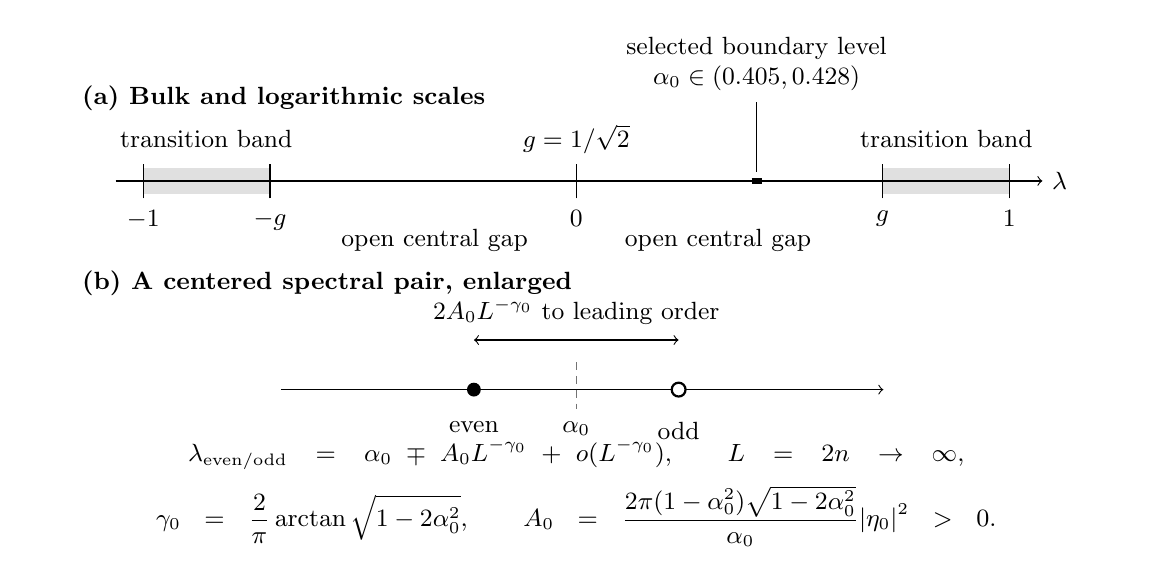
\begin{tikzpicture}[x=1cm,y=1cm,font=\small]
  \node[anchor=west,font=\small\bfseries] at (-6.4,1.05)
    {(a) Bulk and logarithmic scales};
  \fill[black!12] (-5.5,-0.16) rectangle (-3.889,0.16);
  \fill[black!12] (3.889,-0.16) rectangle (5.5,0.16);
  \draw[->] (-5.85,0) -- (5.92,0) node[right] {$\lambda$};
  \foreach \x/\lab in {-5.5/{-1},-3.889/{-g},0/{0},3.889/{g},5.5/{1}} {
    \draw (\x,-0.22) -- (\x,0.22);
    \node[anchor=north] at (\x,-0.25) {$\lab$};
  }
  \node at (-4.7,0.53) {transition band};
  \node at (4.7,0.53) {transition band};
  \node at (0,0.53) {$g=1/\sqrt2$};
  \node at (-1.8,-0.75) {open central gap};
  \node at (1.8,-0.75) {open central gap};
  \draw[line width=2pt] (2.2275,0) -- (2.354,0);
  \draw (2.29,0.12) -- (2.29,1.00);
  \node[anchor=south,align=center] at (2.29,1.02)
    {selected boundary level\\$\alpha_0\in(0.405,0.428)$};
  \node[anchor=west,font=\small\bfseries] at (-6.4,-1.30)
    {(b) A centered spectral pair, enlarged};
  \draw[->] (-3.75,-2.65) -- (3.9,-2.65);
  \draw[densely dashed,black!55] (0,-2.30) -- (0,-2.90);
  \node[anchor=north] at (0,-2.94) {$\alpha_0$};
  \fill (-1.30,-2.65) circle (2.5pt);
  \draw[fill=white,line width=0.8pt] (1.30,-2.65) circle (2.5pt);
  \node[anchor=north] at (-1.30,-2.94) {even};
  \node[anchor=north] at (1.30,-2.94) {odd};
  \draw[<->] (-1.30,-2.02) -- (1.30,-2.02);
  \node[anchor=south] at (0,-1.95) {$2A_0L^{-\gamma_0}$ to leading order};
  \node[align=center,text width=13.7cm] at (0,-3.96) {
    $\displaystyle
    \lambda_{\mathrm{even/odd}}
       =\alpha_0\mp A_0L^{-\gamma_0}+o(L^{-\gamma_0}),\qquad L=2n\to\infty,$\\[5pt]
    $\displaystyle
    \gamma_0=\frac2\pi\arctan\sqrt{1-2\alpha_0^2},\qquad
    A_0=\frac{2\pi(1-\alpha_0^2)\sqrt{1-2\alpha_0^2}}{\alpha_0}
          |\eta_0|^2>0.$};
\end{tikzpicture}
\caption{Spectral scales for the single-frequency operator.
The shaded bands support the logarithmic trace density, whereas the
bulk values are $\pm1$. The marked interval encloses the certified
phase-zero half-line level; it is not a census of the central gaps.
The enlarged panel shows the leading locations of the two eigenvalues
of $\mathcal K_n$ converging to that level. Their placement is schematic,
not numerical data. Here $\eta_0$ is the normalized physical tail
amplitude. The coefficient includes the complementary-resolvent
contribution, and $|\eta_0|>1/100$ makes it nonzero.}
\label{fig:unified-spectral-roadmap}
\end{figure}

\tableofcontents
\section{Exchange structure and critical scaling}\label{unified:sec:foundations}
\begingroup
\let\section\subsection
\let\subsection\subsubsection
\section{The two operators and their exchange representations}\label{sec:matrix}
On $L^2(\mathbb T)$, $\mathbb T=\mathbb R/\mathbb Z$, put
$e_m(t)=e^{2\pi imt}$ and let $P_N$ project onto
$V_N=\operatorname{span}\{e_m:|m|\le N\}$.  For $\delta=1-\varepsilon$,
define
\[
 (S_\delta f)(t)=\mathbf1_{[\delta,1]}(t)f(t-\delta),
 \qquad T_\delta=S_\delta+S_\delta^*.
\]
$S_\delta$ carries the source arc $[0,\varepsilon]$ onto the target arc
$[1-\varepsilon,1]$; these are disjoint because $\varepsilon<1/2$. Thus
$T_\delta$ exchanges them, vanishes off their union, and has norm one.

\begin{lemma}\label{lem:source-block}
The matrix of $P_NT_\delta P_N$ is \eqref{eq:2.1}.  At the critical scale,
\begin{equation}\label{eq:2.2}
 A_N(\tau/N)_{mn}=N^{-1}K_\tau(m/N,n/N).
\end{equation}
In particular $\|A_N(\varepsilon)\|\le1$.
\end{lemma}
\begin{proof}
The matrix entry of $S_{1-\varepsilon}$ is
$e^{2\pi im\varepsilon}\int_0^\varepsilon e^{2\pi i(n-m)t}\,dt$;
the adjoint entry has the same integral multiplied by
$e^{-2\pi in\varepsilon}$.  Their sum gives \eqref{eq:2.1}, including the
diagonal.  Substitution gives \eqref{eq:2.2}.
\end{proof}

Write $\mathcal Rf(x)=f(-x)$, $(\mathcal R_Na)_m=a_{-m}$ and
$\mathcal H_p=\ker(\mathcal R-pI)$ for $p=\pm1$.
The largest and smallest spectral values in these sectors are denoted by
$\lambda_p^\pm(\tau)$ for $\mathcal K_\tau$ and by $\lambda_{N,p}^\pm(\varepsilon)$
for $A_N(\varepsilon)$;
$F_p(\tau)=\|\mathcal K_\tau|_{\mathcal H_p}\|$.
We use the unitary Fourier transform
$(\mathcal Ff)(\xi)=\widehat f(\xi)=\int_{\mathbb R}f(x)e^{2\pi ix\xi}\,dx$
throughout.
Let $E$ extend functions on $[-1,1]$ by zero and put $U=\mathcal FE$.

\begin{proposition}[Cross-window structure]\label{thm:crosswindow}\label{prop:traces}
Let $R_\tau$ denote multiplication by $\mathbf1_{(-\tau,\tau)}$ on
$L^2(\mathbb R)$ and
\begin{equation}\label{eq:v6:4.1}
 (J_\tau g)(\xi)=
 \begin{cases}g(\xi-\tau),&0<\xi<\tau,\\
 g(\xi+\tau),&-\tau<\xi<0,\\0,&|\xi|\ge\tau.
 \end{cases}
\end{equation}
Then $J_\tau=J_\tau^*$, $J_\tau^2=R_\tau$, and
\begin{equation}\label{eq:v6:4.2}
 \mathcal K_\tau=U^*J_\tau U,\qquad
 \langle f,\mathcal K_\tau f\rangle
 =2\operatorname{Re}\int_0^\tau
 \overline{\widehat f(\xi-\tau)}\widehat f(\xi)\,d\xi.
\end{equation}
Define $C_\theta$ to have kernel
$c_\theta(x-y)=\sin(\pi\theta(x-y))/[\pi(x-y)]$ on $[-1,1]$.
With $\Pi_\pm=(R_\tau\pm J_\tau)/2$ and $C_\pm=U^*\Pi_\pm U$,
\begin{equation}\label{eq:positive-split}
 C_\pm\ge0,\qquad C_++C_-=C_{2\tau},\qquad
 C_+-C_-=\mathcal K_\tau,\qquad \mathcal K_\tau^2\le C_{2\tau}.
\end{equation}
$\mathcal K_\tau$ is trace class with $\|\mathcal K_\tau\|_1\le4\tau$, and
\begin{equation}\label{eq:2.8}
 \tr\mathcal K_\tau=\frac{2\sin(2\pi\tau)}\pi,\qquad
 \tr(\mathcal K_\tau|_{\mathcal H_p})
 =\frac{\sin(2\pi\tau)+p\Si(2\pi\tau)}\pi,
\end{equation}
where $\Si(x)=\int_0^x\sin(t)\,t^{-1}\,dt$.
Moreover $\|\mathcal K_\tau\|<1$ for every finite $\tau>0$.
\end{proposition}
\begin{proof}
Direct Fourier integration yields \eqref{eq:v6:4.2}; equivalently, commuting
the multiplier $i\operatorname{sgn}\xi$ of the Hilbert transform on
$\mathbb R$ with the two frequency shifts in the sine, then compressing to
$[-1,1]$, gives $J_\tau$.
The operators $\Pi_\pm$ are orthogonal projections.  The restriction
$A=R_\tau U:L^2[-1,1]\to L^2(-\tau,\tau)$ is Hilbert--Schmidt with
$\|A\|_2^2=4\tau$.  Thus $C_\pm=A^*\Pi_\pm A$ are positive trace class,
their sum is $A^*A=C_{2\tau}$, and their total trace is $4\tau$.
Also $U^*J_\tau UU^*J_\tau U\le U^*J_\tau^2U=C_{2\tau}$.
Since $C_\pm$ and $\tfrac12(I+p\mathcal R)C_\sigma$, $p,\sigma=\pm1$, are
positive trace-class operators with continuous kernels, their traces are the integrals of their
diagonals (Mercer).  Hence
$\tr\mathcal K_\tau=\int_{-1}^1 2\tau\cos(2\pi\tau x)\,dx$,
$\tr(\mathcal R\mathcal K_\tau)=\int_{-1}^1\sin(2\pi\tau x)/(\pi x)\,dx
 =2\Si(2\pi\tau)/\pi$,
and $\tr(\mathcal K_\tau|_{\mathcal H_p})=\tfrac12[\tr\mathcal
K_\tau+p\,\tr(\mathcal R\mathcal K_\tau)]$ proves \eqref{eq:2.8}.
If $\mathcal K_\tau$ had an eigenvalue of modulus one, equality in the
contraction $U^*J_\tau U$ would force $Uf$ to vanish outside $(-\tau,\tau)$.
The Fourier transform of a compactly supported function is entire, so this
forces $f=0$, a contradiction.
\end{proof}

The same exchange identifies exactly where compression loses mass.
Let $\mathcal G_\tau=\mathcal F^*J_\tau\mathcal F$, $P=EE^*$, and
$\widetilde{\mathcal K}_\tau=\mathcal G_\tau E$.
Since $J_\tau^2=R_\tau$, Plancherel gives
$\widetilde{\mathcal K}_\tau^*\widetilde{\mathcal K}_\tau=C_{2\tau}$ and
\begin{equation}\label{unified:eq:two-leakages}
\begin{aligned}
 C_{2\tau}-\mathcal K_\tau^2
   &=E^*\mathcal G_\tau(I-P)\mathcal G_\tau E\ge0,\\
 1-\|\mathcal K_\tau f\|^2
   &=\|(I-P)\widetilde{\mathcal K}_\tau f\|^2
      +\int_{|\xi|>\tau}|\widehat{Ef}(\xi)|^2\,d\xi
      \qquad(\|f\|=1).
\end{aligned}
\end{equation}
The two terms are output escaping the physical interval and input outside
the frequency band. For an eigenvector the left side is $1-\lambda^2$.
These identities follow by inserting $P+(I-P)=I$; the band has width
$2\tau$, so its concentration kernel is $\sin(2\pi\tau(x-y))/[\pi(x-y)]$.

The elementary identity
\begin{equation}\label{eq:2.4}
 K_\tau(x,y)=2\operatorname{Re}\int_0^\tau
 e^{2\pi i[x(\tau-s)+ys]}\,ds
 =2\cos(\pi\tau(x+y))c_\tau(x-y)
\end{equation}
will be used repeatedly.

\begin{theorem}[Continuum inertia and strict monotonicity]
\label{thm:rev:structure:inertia}\label{thm:rev:structure:monotonicity}
For every $\tau>0$, $\mathcal K_\tau$ is injective and has infinitely many
positive and infinitely many negative eigenvalues in each parity sector.
Write $\xi_{k,p}^+(\tau)>0$ for the positive eigenvalues in
nonincreasing order and $\xi_{k,p}^-(\tau)<0$ for the negative
eigenvalues in nondecreasing order, counting multiplicity; thus
$\xi_{1,p}^{\pm}=\lambda_p^{\pm}$.
For every $k\ge1$, $p=\pm1$ and $0<\tau_1<\tau_2$,
\begin{equation}\label{eq:monotonicity}
\begin{split}
 0&<\xi_{k,p}^+(\tau_1)<\xi_{k,p}^+(\tau_2)<1,\\
 -1&<\xi_{k,p}^-(\tau_2)<\xi_{k,p}^-(\tau_1)<0.
\end{split}
\end{equation}
Each ordered eigenvalue is continuous in $\tau$, tends to zero as
$\tau\downarrow0$, and tends to its respective sign as $\tau\to\infty$.
\end{theorem}
These statements do not assert simplicity at every parameter.
\begin{proof}
Both $A=R_\tau U$ and $A^*$ are injective: the Fourier transform of a
function supported in either bounded interval is entire, and cannot vanish
on the other interval unless it vanishes identically.  In the polar
decomposition $A=BV$, $B=(AA^*)^{1/2}$ is therefore positive and injective,
$V$ is unitary, and both respect reflection.  The last assertion follows
from $A\mathcal R=\mathcal R A$ between the two spaces and uniqueness of
the polar decomposition.  Thus $\mathcal K_\tau$ is unitarily equivalent,
sector by sector, to $BJ_\tau B$.  This proves injectivity.

In each parity sector the involution $J_\tau$ on $L^2(-\tau,\tau)$ has
infinite-dimensional eigenspaces of both signs: for any $p,\sigma=\pm1$,
choose $h\in L^2(0,\tau)$ with $h(\tau-\xi)=\sigma p h(\xi)$, and set
$g=h$ on $(0,\tau)$ and $g(\xi)=\sigma h(\xi+\tau)$ on $(-\tau,0)$.
Then $J_\tau g=\sigma g$ and $\mathcal Rg=pg$.  The range of $B$ is dense
in either parity sector.  Approximate any $n$ orthonormal vectors in this
joint eigenspace by $Bf_1,\ldots,Bf_n$ with $f_j\in\mathcal H_p$.  The matrix
$(\sigma\langle Bf_i,J_\tau Bf_j\rangle)_{i,j}$ can be made arbitrarily close
to the identity, hence positive definite.  The minimax principle gives at
least $n$ eigenvalues of sign $\sigma$ for $BJ_\tau B$ on the sector $p$.

For monotonicity use the parity-preserving isometry
$\mathcal D_af(x)=a^{-1/2}f(x/a)\mathbf1_{[-a,a]}(x)$, $0<a<1$.
The kernel gives
$\mathcal D_a^*\mathcal K_\tau\mathcal D_a=\mathcal K_{a\tau}$.
Fix $k,p,\sigma$, with $\sigma=\pm1$, and let $c>0$ be the $k$th
largest eigenvalue of $\sigma\mathcal K_{a\tau}|_{\mathcal H_p}$.
The dilated span $M$ of its first $k$ eigenvectors has dimension $k$,
and every unit vector in $M$ has Rayleigh quotient at least $c$ for
$\sigma\mathcal K_\tau$.  Minimax gives weak monotonicity.  If the
$k$th largest eigenvalue at $\tau$ were also $c$, the spectral subspace
$E$ of $\sigma\mathcal K_\tau|_{\mathcal H_p}$ for eigenvalues strictly
larger than $c$ would have dimension at most $k-1$.  There would be a
unit vector $v\in M\cap E^\perp$.  Its Rayleigh quotient is at least
$c$ because $v\in M$ and at most $c$ because $v\in E^\perp$.
Equality and the spectral theorem force
$\sigma\mathcal K_\tau v=cv$.  Every nonzero eigenfunction is analytic,
because the kernel is entire in its first variable, locally uniformly
in its second.  But $v$ vanishes on $(a,1)$, a contradiction.  This proves
strict monotonicity for both signs; strict contractivity gives the outer
inequalities in \eqref{eq:monotonicity}.
Norm continuity of the kernel and the minimax principle give continuity
of each ordered eigenvalue, and $\|\mathcal K_\tau\|\le4\tau$ gives
the limit at zero.  For the limit at infinity use the full-line operator
$\mathcal G=\mathcal F^*J\mathcal F$ of Section~\ref{sec:crosswindow}.
The construction above with $\tau=1$ gives infinitely many orthonormal
eigenvectors of $J$ of either sign and either reflection parity. Their
inverse Fourier transforms give the same eigenspaces for $\mathcal G$.
Fix $k$ orthonormal vectors $g_1,\ldots,g_k$ of sign $\sigma$ and parity $p$.
For $P_\tau=P_{(-\tau,\tau)}$, strong convergence $P_\tau\to I$ gives
\[
 \bigl(\langle P_\tau g_i,P_\tau g_j\rangle\bigr)_{i,j}\to I_k,
 \qquad
 \bigl(\sigma\langle P_\tau g_i,\mathcal G P_\tau g_j\rangle\bigr)_{i,j}
 \to I_k.
\]
The truncated vectors retain parity $p$. Thus every unit vector in their
span has Rayleigh quotient for $\sigma\mathcal G$ tending uniformly to one.
The dilation identity in Section~\ref{sec:crosswindow} and minimax imply
$\liminf_{\tau\to\infty}|\xi_{k,p}^{\sigma}(\tau)|\ge1$.
Contractivity supplies the reverse bound, proving the asserted limits.
\end{proof}

\subsection{The global exchange and its Bloch symbol}\label{sec:crosswindow}
On $L^2(\mathbb R)$ define
\[
 (Jg)(\xi)=\mathbf1_{(0,1)}(\xi)g(\xi-1)
              +\mathbf1_{(-1,0)}(\xi)g(\xi+1),\qquad
 \mathcal G=\mathcal F^*J\mathcal F.
\]
Then $J=J^*$, $J^2=\mathbf1_{(-1,1)}$ and $\|J\|=1$.
For compactly supported inputs, the two Fourier integrals give the kernel
\[
 G(X,Y)=2\cos(\pi(X+Y))\frac{\sin(\pi(X-Y))}{\pi(X-Y)}
       =\frac{\sin(2\pi X)-\sin(2\pi Y)}{\pi(X-Y)}.
\]
In particular $\mathcal G^2=\mathcal F^*\mathbf1_{(-1,1)}\mathcal F$
and $G(X+1,Y+1)=G(X,Y)$.

Dilation gives the identities
\[
 (\mathcal D_\tau f)(X)=\tau^{-1/2}f(X/\tau),\qquad
 \mathcal D_\tau\mathcal K_\tau\mathcal D_\tau^*
 =P_{(-\tau,\tau)}\mathcal G P_{(-\tau,\tau)}.
\]
Here $P_I$ multiplies by $\mathbf1_I$; the dilated kernel is
$\tau^{-1}K_\tau(X/\tau,Y/\tau)=G(X,Y)$.
The trace-class property, the norm bound and the trace formulas are in
Proposition~\ref{prop:traces}.

\begin{proposition}[Exact Bloch symbol]\label{T4:prop:bloch}
Identify $L^2(\mathbb R)$ with $\ell^2(\mathbb Z;H)$, $H=L^2(0,1)$,
by $f_n(t)=f(n+t)$.  Then $\mathcal G$ is the Laurent operator with blocks
\begin{equation}\label{T4:eq:symbol}
 g_k(t,s)=G(k+t,s)=\int_0^1\varsigma(\theta)(t,s)e^{-2\pi ik\theta}\,d\theta,
 \quad
 \varsigma(\theta)(t,s)=2\cos(\pi(t+s))e^{i\pi(t-s)(1-2\theta)}.
\end{equation}
For $e_j(t)=e^{2\pi ijt}$ and $W_\theta=M_{e^{2\pi i\theta t}}$,
\[
 \varsigma(\theta)=W_\theta^*X_{1,0}W_\theta,
 \qquad X_{j,k}=|e_j\rangle\langle e_k|+|e_k\rangle\langle e_j|.
\]
It has eigenvalues $1,-1,0$ and one jump on the circle:
$\varsigma(0)=X_{1,0}$, $\varsigma(1)=X_{0,-1}$.
\end{proposition}
\begin{proof}
Periodicity gives the cell blocks $G(k+t,s)$.  With $z=t-s$,
\[
 \int_0^1e^{i\pi z(1-2\theta)}e^{-2\pi ik\theta}\,d\theta
 =\frac{\sin(\pi z)}{\pi(k+z)}.
\]
The removable case $k=z=0$ follows by continuity.  Multiplication by
$2\cos(\pi(t+s))$ proves \eqref{T4:eq:symbol}; Fubini is valid because
the kernels are bounded on the unit square.  Expanding the cosine
expresses the symbol as the exchange of the orthonormal pair
$e^{2\pi i(1-\theta)t},e^{-2\pi i\theta t}$, proving the rest.
\end{proof}
The jump is not removable by a continuous periodic gauge to a constant
symbol: its two endpoint limits would then be conjugated by the same
unitary and would have to coincide.  The proof below instead uses a
nonconstant symbol on a fixed three-dimensional subspace.



\section{Critical-window convergence}\label{sec:critical}

\begin{theorem}[Explicit operator-norm limit]\label{thm:nystrom}
For every $0<T<\infty$ and every integer $N>2T$, which ensures that
$\tau/N<1/2$ for $0\le\tau\le T$, there are
reflection-intertwining isometries $U_N$ from
$\mathbb C^{2N+1}$ into $L^2[-1,1]$, independent of $\tau$, under which the
embedded matrix $\widetilde A_{N,\tau}=U_NA_N(\tau/N)U_N^*$ acts as zero off
its step-function range and
\begin{equation}\label{eq:3.1}
 \sup_{0\le\tau\le T}
 \|\widetilde A_{N,\tau}-\mathcal K_\tau\|
 \le \frac{2T+8\pi T^2}{N}.
\end{equation}
Pointwise in $\tau$, the numerator may be replaced by
$2\tau+8\pi\tau^2$.  The same estimate holds in each parity sector.
\end{theorem}

\begin{proof}
Put $h=2/d$, and partition $[-1,1]$ into equal cells $B_m$
of width $h$ centered at $z_m=hm$, $-N\le m\le N$.  Define
$(U_Na)(x)=h^{-1/2}a_m$ on $B_m$.  Since
$N^{-1}=h(2N+1)/(2N)$, the embedded matrix has step kernel
\begin{equation}\label{eq:3.2}
 \widetilde K_{N,\tau}(x,y)
 =\frac{2N+1}{2N}K_\tau(m/N,n/N),
 \quad (x,y)\in B_m\times B_n.
\end{equation}
Formula \eqref{eq:2.4} gives
\begin{equation}\label{eq:3.3}
 |K_\tau|\le2\tau,\qquad
 |\partial_xK_\tau|,|\partial_yK_\tau|\le2\pi\tau^2.
\end{equation}
Since $z_m=hm$ and $|z_m-m/N|=|m|/(N(2N+1))\le1/(2N+1)=h/2$, while
$|x-z_m|\le h/2$ on $B_m$, we have $|x-m/N|\le h$.  The scalar mismatch in
\eqref{eq:3.2} and
the two coordinate errors therefore give
\[
 |\widetilde K_{N,\tau}(x,y)-K_\tau(x,y)|
 \le\frac{\tau+4\pi\tau^2}{N}.
\]
The square $[-1,1]^2$ has area $4$, so the operator norm is at most the
Hilbert--Schmidt norm, which is at most twice this supremum.  Reflection
intertwining follows from the symmetric cells.
\end{proof}

Differentiating \eqref{eq:2.4} also gives
\begin{equation}\label{eq:3.4}
 \|\mathcal K_\tau-\mathcal K_{\tau'}\|
 \le(4+8\pi T)|\tau-\tau'|,
 \qquad 0\le\tau',\tau\le T.
\end{equation}
Hence if $\tau_N=N\varepsilon_N\to\tau<\infty$, then with
$T=\sup_N\tau_N<\infty$ and every $N>2T$,
\begin{equation}\label{eq:3.5}
 \|\widetilde A_{N,\tau_N}-\mathcal K_\tau\|
 \le\frac{2\tau_N+8\pi\tau_N^2}{N}
 +(4+8\pi T)|\tau_N-\tau|\longrightarrow0.
\end{equation}
The parity norms and every isolated nonzero parity spectral cluster therefore
converge; the same holds for an individual signed edge whenever it is separated
from zero.


\endgroup
\section{Uniform trace laws and their coefficients}\label{unified:sec:trace}
\begingroup
\let\section\subsection
\let\subsection\subsubsection
\section{The logarithmic density and spectral counts}\label{v6:sec:density}
\begin{proposition}[Density and even moments]\label{T10:prop:density}
For H\"older $f$,
\begin{equation}\label{T10:eq:density}
 \varkappa(f)=\int_{1/\sqrt2}^1
 [f(x)+f(-x)-f(1)-f(-1)]\varpi(x)\,dx,
 \quad
 \varpi(x)=\frac{2x}{\pi^2(1-x^2)\sqrt{2x^2-1}}.
\end{equation}
For integers $m\ge1$,
\begin{equation}\label{T10:eq:moments}
 \pi^2\varkappa(x^{2m})=
 \sum_{j=1}^m \binom{m}{j}(-2)^j\frac{(j-1)!^2}{(2j-1)!},
 \qquad \varkappa(x^{2m+1})=0.
\end{equation}
\end{proposition}
\begin{proof}
The two halves of the $t$ integral in \eqref{T10:eq:kappa} coincide.
On either half substitute $x=\sqrt{1-2t(1-t)}$ to obtain the density.
Its singularity at $1/\sqrt2$ is integrable; at $1$ the endpoint
subtraction supplies the H\"older factor.  For the moments expand
$(1-2t(1-t))^m-1$ and integrate each term using
$B(j,j)=(j-1)!^2/(2j-1)!$.  Odd tests cancel identically.
\end{proof}
Thus the coefficients for $x^2,x^4,x^6$ are respectively
$-2,-10/3,-64/15$ in units of $\pi^{-2}$.  In particular
Theorem~\ref{T10:conj:law}, applied to the $C^2$ test $f(x)=x^2-x^4$, for
which $f(0)=0$ and $f(1)+f(-1)=0$, gives
\begin{equation}\label{short:eq:quartic}
 \operatorname{tr}(\mathcal K_\tau^2-\mathcal K_\tau^4)
 =\frac4{3\pi^2}\log\tau+O(1).
\end{equation}
The gap comes from the jump, not from the physical spectrum. The two
one-sided exchanges interpolate as
\[
 M_t=(1-t)X_{0,-1}+tX_{1,0}
 =\begin{pmatrix}0&1-t&0\\1-t&0&t\\0&t&0\end{pmatrix},
 \qquad\operatorname{spec}M_t=\{0,\pm r_t\}.
\]
Thus the jump trace is $f(r_t)+f(-r_t)-f(1)-f(-1)$, giving
\eqref{T10:eq:kappa} in the Widom normalization \cite{Widom1982}.
In contrast, the gauge symbol $a(\theta)$ in
Section~\ref{app:general-trace} has values $0,\pm1$ at every $\theta$.
The classical prolate interpolation traverses $[0,1]$; here the moving
values stay in the two outer bands. The subtraction at $\pm1$ is essential
because $\varpi$ has infinite mass there.

\subsection{Band-local regularity and the trace norm}
\label{v7:sec:regularity}

Put $g=2^{-1/2}$ and retain $C_V,C_*,B_1,B_2$ and the strip constant
$b(\cdot)$ of \eqref{rev5:eq:strip-function} from
Section~\ref{app:general-trace}.  Define
\[
 A_{\rm band}=2C_V+4b(1/2)+2+\frac{2\log(5/2)}{\pi^2}
                 +\sqrt2(C_*+B_1+B_2).
\]
Here $C^{1,1}$ means continuously differentiable with Lipschitz derivative,
using one-sided derivatives at an interval's endpoints.
Trace asymptotics for test functions with finitely many H\"older
singularities are treated in \cite{LeschkeSobolevSpitzer2017,Sobolev2017}
and \cite[Theorem~4.22]{BollmannMueller2024}, with remainders of lower
order than the logarithmic term.  The hypothesis below is of a different
kind: beyond a global Lipschitz bound, no regularity is imposed inside the
central gap, which the exact gap of the model makes possible.

\begin{theorem}[Regularity only on the model bands]
\label{v7:thm:band-regularity}
Let $f:[-1,1]\to\mathbb R$ be $L$-Lipschitz, with $f(0)=0$.
Suppose its restrictions to $[-1,-g]$ and $[g,1]$ are $C^{1,1}$,
and let $M$ be the larger Lipschitz constant of their derivatives.
Then, for $\tau\ge2$,
\[
 \left|\tr f(\mathcal K_\tau)
       -2\tau[f(1)+f(-1)]-\varkappa(f)\log\tau\right|
 \le A_{\rm band}L+B_2M.
\]
For the phase-shifted operator $\mathcal K_{\tau,\phi}$ of
Proposition~\ref{v6:prop:allphase}, the same estimate holds uniformly in $\phi$
with $A_{\rm band}$ replaced by $A_{\rm band}+4b(1/2)$.
\end{theorem}
\begin{proof}
In the scalar model write $C=T_n(c)$ and $S=T_n(s)$.
Since $c+s\ge1$, $C+S\ge I$ and
$H_n=C^2+S^2=[(C+S)^2+(C-S)^2]/2\ge I/2$.
Thus $D_n(u)+D_n(v)=I-H_n$ and $D_n(v_0)$ have spectra in $[0,1/2]$,
the latter by \eqref{rev5:eq:half-bound}. The star consequently has
exactly $n$ eigenvalues of each sign, all of magnitude at least $g$.
For $h$ of \eqref{rev5:eq:h}, restricted to $0\le x\le1/2$, put
$r=\sqrt{1-x}$. Then
\[
 h'=\frac{f'(-r)-f'(r)}{2r},\qquad
 h''=\frac{f''(r)+f''(-r)}{4r^2}
       -\frac{f'(r)-f'(-r)}{4r^3}\quad\text{a.e.}
\]
Hence $h\in C^{1,1}$, $h(0)=0$,
$\operatorname{Lip}(h)\le\sqrt2L$ and
$\operatorname{Lip}(h')\le M+\sqrt2L$; integrate the a.e. bound on $h''$
to obtain the last assertion. Scalar Taylor remainder is therefore
bounded by $(M+\sqrt2L)|x-y|^2/2$, so the spectral-measure proof of
Lemma~\ref{rev5:lem:compression} applies to $h$.
Extend it affinely from $1/2$ to $1$, preserving its Lipschitz bound;
all second-derivative estimates and spectral evaluations remain in
$[0,1/2]$. Signed singular-value pairing gives exactly
\[
 \tr f(T_n(a))=n[f(1)+f(-1)]+\tr h(D_n(u)+D_n(v)).
\]
Equations~\eqref{rev5:eq:star-transfer},
\eqref{rev5:eq:star-defect-error} and \eqref{rev5:eq:model-trace}
now bound the error at $n=2q$ by
$2C_VL+(C_*+B_1)\sqrt2L+B_2(M+\sqrt2L)$.
Integer transfer, bulk adjustment and \eqref{rev5:eq:kappa-bound} add
$[4b(1/2)+2+2\pi^{-2}\log(5/2)]L$, giving $A_{\rm band}$.
The phase comparison adds $4b(1/2)L$.
\end{proof}

\begin{corollary}[Schatten norms and a sharp coefficient bound]\label{cor:schatten}\label{v7:cor:trace-norm}
For $p\ge1$ put
\[
 \varkappa_p=\varkappa(|x|^p)
 =\frac1{\pi^2}\int_0^1\frac{r_t^{\,p}-1}{t(1-t)}\,dt<0 .
\]
Then $\|\mathcal K_\tau\|_p^p=4\tau+\varkappa_p\log\tau+O_p(1)$ as
$\tau\to\infty$, and $p\mapsto\varkappa_p$ is strictly decreasing and convex.
For $p=1$ the remainder has modulus at most $A_{\rm band}$ for $\tau\ge2$.
The coefficients at $p=1$ and $p=3$ are
\begin{align*}
 \varkappa_1&=-\frac2{\pi^2}\bigl[\sqrt2\log(1+\sqrt2)-\log2\bigr]
   =-0.112122\ldots,\\
 \varkappa_3&=-\frac2{\pi^2}\Bigl[\tfrac12-\log2
      +\tfrac5{2\sqrt2}\log(1+\sqrt2)\Bigr]=-0.276589\ldots,
\end{align*}
and $\varkappa_{2m}$ is given by \eqref{T10:eq:moments}.  Moreover, for every
Lipschitz $f$,
\begin{equation}\label{eq:kappa-sharp}
 |\varkappa(f)|\le|\varkappa_1|\operatorname{Lip}(f),
\end{equation}
with equality for $f(x)=|x|$.  This sharpens the crude bound
\eqref{rev5:eq:kappa-bound} by the factor $2/(\pi^2|\varkappa_1|)=1.8073$.
\end{corollary}
\begin{proof}
For $p\ge1$ the function $|x|^p$ is Lipschitz on $[-1,1]$ and smooth away from
the origin, so Theorem~\ref{v7:thm:band-regularity} applies and gives the
expansion with $f(1)+f(-1)=2$.  The displayed integral is
\eqref{T10:eq:kappa} for an even $f$.  Since $r_t<1$ off the endpoints,
$p\mapsto r_t^{\,p}$ is strictly decreasing and convex, and these properties
pass through the positive weight $[t(1-t)]^{-1}$.  For $p=1$, $L=1$ and $M=0$ in the band-local theorem.
Rationalizing $r_t-1$ in \eqref{T10:eq:kappa} and setting $u=2t-1$, the
integrand being even in $u$, gives
\[
 \varkappa(|x|)=-\frac2{\pi^2}
       \int_0^1\frac{du}{1+\sqrt{(1+u^2)/2}}.
\]
For $u=\sinh v$ and $V=\log(1+\sqrt2)$ the integral equals
$\sqrt2\,V-2\int_0^V(\sqrt2+\cosh v)^{-1}\,dv$.
Substitution $z=\tanh(v/2)$ evaluates the last integral as
$2\operatorname{artanh}((\sqrt2-1)^2)=\tfrac12\log2$.

For $p=3$ the same substitution
$u=2t-1$, with $r=\sqrt{(1+u^2)/2}$ and
$r^3-1=(r-1)(1+r+r^2)$, gives
\[
 \varkappa_3=-\frac2{\pi^2}\int_0^1\frac{1+r+r^2}{1+r}\,du,
\]
which is the stated closed form, since $(1+r+r^2)/(1+r)=r+(1+r)^{-1}$ and
$\int_0^1r\,du=\tfrac12+\log(1+\sqrt2)/(2\sqrt2)$.
For \eqref{eq:kappa-sharp} bound each of $|f(\pm r_t)-f(\pm1)|$ by
$\operatorname{Lip}(f)(1-r_t)$ in \eqref{T10:eq:kappa} and compare with the
same integral for $|x|$, which realizes both bounds with equality.
\end{proof}

The explicit logarithmic coefficients proved in this paper are collected in
Table~\ref{tab:coefficients}.

\begin{table}[htbp]
\centering
\begin{tabular}{llll}
\hline
statistic & test $f$ & bulk & $\varkappa(f)$\\
\hline
trace norm & $|x|$ & $4\tau$ & $-0.112122$\\
squared Hilbert--Schmidt norm & $x^2$ & $4\tau$ & $-2/\pi^2=-0.202642$\\
Schatten $\|\cdot\|_3^3$ & $|x|^3$ & $4\tau$ & $-0.276589$\\
Schatten $\|\cdot\|_4^4$ & $x^4$ & $4\tau$ & $-10/(3\pi^2)=-0.337737$\\
quartic defect & $x^2-x^4$ & $0$ & $4/(3\pi^2)=+0.135094$\\
$\log\det(I+\mathcal K_{\tau,\phi}^2)$ & $\log(1+x^2)$ & $4\tau\log2$ & $-1/9$\\
\hline
\end{tabular}
\caption{Bulk and logarithmic coefficients of Theorem~\ref{T10:conj:law}.
Every entry is exact; decimals truncate the closed forms of
Corollary~\ref{cor:schatten},
Proposition~\ref{T10:prop:density} and Remark~\ref{rem:det-square}.  The
last row concerns the phase-shifted operator $\mathcal K_{\tau,\phi}$ of
Proposition~\ref{v6:prop:allphase}, for which the same law holds uniformly
in $\phi$.}
\label{tab:coefficients}
\end{table}

\subsection{Gap counts and transition quantiles}\label{v7:sec:quantiles}
Let $\mu_j^\pm(\tau)$ be the positive eigenvalues and the magnitudes of
negative eigenvalues, respectively, in nonincreasing order with multiplicity.
Both lists are infinite. They include both reflection sectors.
Set $N_\pm(a;\tau)=\#\{j:\mu_j^\pm(\tau)>a\}$ and $C_0=2C_V+4b(1/2)$.
\begin{proposition}[Gap mass and the count plateau]
\label{v7:prop:gap-mass}\label{v7:prop:count-plateau}
For $w_g(x)=\min\{|x|,(g-|x|)_+\}$ and $\tau\ge2$,
\[
 \sum_jw_g(\lambda_j(\mathcal K_\tau))\le C_0,\qquad
 \sum_{|\lambda_j|\le a}|\lambda_j|
 \le C_0\max\{1,a/(g-a)\}\quad(0<a<g).
\]
For either sign and $0<a<g$,
\begin{equation}\label{v7:eq:count-plateau}
 2\tau-1-\frac{C_0}{g-a}\le N_\pm(a;\tau)
                 \le2\tau+1+\frac{C_0}{a}.
\end{equation}
\end{proposition}
\begin{proof}
For a nearest integer $q$ to $\tau$ put $n=2q$ and $M_n=T_n(a(\cdot))$.
The star has $n$ eigenvalues of each sign in the outer bands and all others
zero. Equations~\eqref{rev5:eq:integer-transfer} and
\eqref{rev5:eq:star-transfer} give
$|\tr F(\mathcal K_\tau)-\tr F(M_n)|\le C_0\operatorname{Lip}(F)$
for every real Lipschitz $F$ with $F(0)=0$.
Apply this first to the nonnegative 1-Lipschitz function $w_g$, which
vanishes on the star spectrum. The second mass bound follows from
$w_g(x)\ge\min\{1,(g-a)/a\}|x|$ for $|x|\le a$.
For positive counts the ramps
$F_a^+(x)=\min\{1,x_+/a\}$ and
$F_a^-(x)=\min\{1,(x-a)_+/(g-a)\}$ bracket $\mathbf1_{(a,1]}$,
have Lipschitz constants $1/a,1/(g-a)$, and both have star trace $n$.
Reflection gives the negative count; $|n-2\tau|\le1$ finishes the proof.
\end{proof}

\begin{theorem}[Cumulative transition law]\label{v7:thm:cumulative-count}
For $g<a<1$ put
\begin{equation}\label{v7:eq:J}
 J(a)=\int_g^a\varpi(x)\,dx
 =\frac2{\pi^2}\operatorname{artanh}\sqrt{2a^2-1}.
\end{equation}
As $\tau\to\infty$, each sign satisfies
\begin{equation}\label{v7:eq:cumulative-count}
 N_\pm(a;\tau)=2\tau-J(a)\log\tau
                    +O((\log\tau)^{2/3}),
\end{equation}
uniformly for $a$ in every fixed compact subset of $(g,1)$.
\end{theorem}
\begin{proof}
Fix $[a_0,a_1]\subset(g,1)$ and
$\delta_0=\min\{(a_0-g)/2,(1-a_1)/2,1\}$.
The quintic step $S(t)=10t^3-15t^4+6t^5$ on $[0,1]$, continued by zero
and one, is nondecreasing and $C^2$, with derivative bounds $15/8,15$.
For $0<\delta\le\delta_0$ the functions
$F^-_{a,\delta}=S((x-a)/\delta)$ and
$F^+_{a,\delta}=S((x-a+\delta)/\delta)$ bracket $\mathbf1_{(a,1]}$.
Their endpoint values are $0,1$, they vanish at zero, and
$\|(F^\pm)'\|_\infty+\|(F^\pm)''\|_\infty\le135/(8\delta^2)$.
With $M=\max_{[a_0-\delta_0,a_1+\delta_0]}\varpi$, the density gives
$|\varkappa(F^\pm_{a,\delta})+J(a)|\le M\delta$.
The trace theorem therefore implies
\[
 |N_+(a;\tau)-2\tau+J(a)\log\tau|
 \le M\delta\log\tau+135C_{\rm tr}/(8\delta^2).
\]
Choose $\delta=\min\{\delta_0,(\log\tau)^{-1/3}\}$.
Reflection gives the other sign and integration of $\varpi$ gives $J$.
\end{proof}

\begin{corollary}[Signed transition quantiles]\label{v7:cor:quantiles}
Fix $\nu\ne0$ and put
$j_\tau=\lfloor2\tau-\nu\log\tau\rfloor$, which is positive for large $\tau$.
For $\nu>0$,
\begin{equation}\label{v7:eq:quantile}
 \mu_{j_\tau}^{\pm}(\tau)=\lambda(\nu)+O_\nu((\log\tau)^{-1/3}),
 \qquad
 \lambda(\nu)=\sqrt{\frac{1+\tanh^2(\pi^2\nu/2)}2}.
\end{equation}
For $\nu<0$, one has
$\mu_{j_\tau}^{\pm}(\tau)=O_\nu((\log\tau)^{-1})$.
\end{corollary}
\begin{proof}
For $\nu>0$, $a_\nu=\lambda(\nu)$ uniquely solves $J(a_\nu)=\nu$.
On a compact neighborhood, $J'=\varpi$ is bounded below by a positive
constant and the counting error is uniform. Writing $L=\log\tau$,
a sufficiently large fixed $D_\nu$ therefore gives
\[
 N_\pm(a_\nu+D_\nu L^{-1/3};\tau)<j_\tau
 \le N_\pm(a_\nu-D_\nu L^{-1/3};\tau).
\]
Strict-count inversion gives the asserted error, including threshold
multiplicities; the floor costs less than one.
For $\nu<0$ put $c=|\nu|$, $a=2(C_0+1)/(cL)$.
Eventually $a<g$, $cL\ge4$, and the plateau gives
$N_\pm(a;\tau)\le2\tau+1+cL/2\le2\tau+cL-1<j_\tau$.
Thus $\mu_{j_\tau}^\pm\le a$.
\end{proof}
No conclusion for the central index $\nu=0$, or for separate reflection
sectors, is asserted by these quantile estimates.

The profile is a fold of the classical Landau--Widom logistic law
\cite{LandauWidom1980}: for $0<t<1/2$,
$J(r_t)=\pi^{-2}\log((1-t)/t)$ and
$\lambda(\nu)=r_{(1+e^{\pi^2\nu})^{-1}}$.
This follows from $\sqrt{2r_t^2-1}=|1-2t|$. The result is the stated
counting and quantile error for both signed physical lists, which need
not themselves be sign-symmetric.

\begin{corollary}[Gap counts and signed transition counts]
\label{rev5:cor:counts}
Eigenvalues below are counted with multiplicity.  For fixed
$0<a\le b<1/\sqrt2$,
\begin{equation}\label{rev5:eq:gap-count}
 \#\{j:a\le|\lambda_j(\mathcal K_\tau)|\le b\}
 \le\frac{C_0}{\min\{a,1/\sqrt2-b\}}\qquad(\tau\ge2).
\end{equation}
For fixed $1/\sqrt2<a<b<1$, each sign separately satisfies
\begin{equation}\label{rev5:eq:band-count}
 \#\{j:\lambda_j(\mathcal K_\tau)\in[a,b]\}
 =I_{a,b}\log\tau+O_{a,b}((\log\tau)^{2/3}),
\end{equation}
and the same formula holds for $[-b,-a]$, where
$I_{a,b}=\int_a^b\varpi(x)\,dx$ and $\varpi$ is given in
Proposition~\ref{T10:prop:density}.  With $v(x)=\sqrt{2x^2-1}$,
\begin{equation}\label{T11:eq:kappaclosed}
 I_{a,b}=\varkappa(\mathbf1_{[a,b]})
 =\frac1{\pi^2}\log
   \frac{(1+v(b))(1-v(a))}{(1-v(b))(1+v(a))},\qquad
 I_{0.72,\,0.995}=0.4967058\ldots .
\end{equation}
Here the indicator notation denotes the convergent density integral;
the trace theorem is applied only to smooth comparison functions.
\end{corollary}

\begin{proof}
On $a\le|x|\le b$ the weight of Proposition~\ref{v7:prop:gap-mass}
is at least $\min\{a,1/\sqrt2-b\}$, proving the gap count.

For the transition interval, put $L=\log\tau$ and
$\delta=L^{-1/3}$. For sufficiently large $\tau$, all thresholds below
lie in a fixed compact subset of $(1/\sqrt2,1)$. The strict counts obey
\[
 N_+(a;\tau)-N_+(b;\tau)
 \le\#\{j:\lambda_j\in[a,b]\}
 \le N_+(a-\delta;\tau)-N_+(b;\tau).
\]
Theorem~\ref{v7:thm:cumulative-count}, uniform on that compact set,
and $J'=\varpi$ bound both sides by
$[J(b)-J(a)]L+O(L^{2/3})$, since
$[J(a)-J(a-\delta)]L=O(\delta L)$.
The same argument for $N_-$ proves the negative interval formula.
This bracketing also covers arbitrary multiplicity at both endpoints.
Finally,
$d[\log((1+v(x))/(1-v(x)))]/dx=\pi^2\varpi(x)$
proves \eqref{T11:eq:kappaclosed}.
\end{proof}

These results concern fixed compact windows.  They do not assert an empty
gap, bounded counts on the whole punctured gap, an $O(1)$ remainder for
sharp transition counts, or uniformity when the endpoints approach
$0$, $1/\sqrt2$ or $1$.  The density integral diverges as $b\uparrow1$.
The exponent $2/3$ comes from this $C^2$ smoothing estimate; no optimality
is claimed.


\subsection{The regularity obstruction}\label{sec:open}
\begin{proposition}[Obstruction to an all-H\"older bounded remainder]
\label{T10:prop:holder-obstruction}
For every $0<\alpha<1$ and every closed interval
$I=[a,b]\subset(1/\sqrt2,1)$ with $a<b$, there is a real
$f\in C^{0,\alpha}([-1,1])$ supported in $I$ for which
\[
 \sup_{n\ge2}\left|
 \operatorname{tr}f(\mathcal K_n)-\varkappa(f)\log n\right|=\infty.
\]
Consequently \eqref{T10:eq:law} cannot hold with an $O_f(1)$ remainder for
every H\"older test function vanishing at zero.
\end{proposition}

\begin{proof}
Let $X$ be the Banach space of real $C^{0,\alpha}$ functions supported
in $I$, with norm $\|f\|_\infty+[f]_\alpha$. On $X$,
$\varkappa(f)=\int_I\varpi f$, where $\min_I\varpi>0$.
The functionals
$L_n(f)=\sum_jf(\lambda_j(\mathcal K_n))-(\log n)\int_I\varpi f$
are continuous: compactness leaves finitely many eigenvalues in $I$.
Their number $m_n$ is $O(\log n)$ by Corollary~\ref{rev5:cor:counts}.
Let $Z_n$ contain those eigenvalues and the endpoints of $I$, and set
$f_n(x)=\operatorname{dist}(x,Z_n)^\alpha$ on $I$, zero elsewhere.
Since distance is 1-Lipschitz and $|r^\alpha-s^\alpha|\le|r-s|^\alpha$,
including across the endpoints, $\|f_n\|_X\le1+(b-a)^\alpha$.
Its spectral sum vanishes. The successive gap lengths $\ell_i$ have sum
$b-a$ and number at most $m_n+1$, so exact integration and convexity give
\[
 \int_I\varpi f_n\ge
 \frac{\min_I\varpi}{2^\alpha(1+\alpha)}\sum_i\ell_i^{1+\alpha}
 \ge\frac{\min_I\varpi(b-a)^{1+\alpha}}
 {2^\alpha(1+\alpha)(m_n+1)^\alpha}.
\]
Thus $\|L_n\|\ge c(\log n)^{1-\alpha}\to\infty$.
Uniform boundedness supplies one fixed $f\in X$ with unbounded remainder.
\end{proof}

This obstruction concerns the combination of the entire H\"older class and
an $O_f(1)$ remainder.  It is compatible with the $C^2$ theorem, its band-local extension, and with the
functional \eqref{T10:eq:kappa}, which is defined on the larger class.
The obstruction lies inside an outer transition band, where
Theorem~\ref{v7:thm:band-regularity} still imposes derivative regularity.
The counting results use admissible smooth or Lipschitz comparison functions.

The remainder cannot be replaced by $c(f)+o(1)$ as $\tau\to\infty$ through
real values: already for $f(x)=x^2$ it contains the term
$-2\pi^{-2}(\log2)\cos(4\pi\tau)$ of Theorem~\ref{thm:hs-exact}, which does
not converge.  Along the integer ladder $\tau=n$ of
Proposition~\ref{T10:prop:holder-obstruction} that term is the constant
$-2\pi^{-2}\log2$.


\section{Resolvent and determinant coefficients}
\begin{proposition}[The resolvent]\label{T10:prop:resolvent}
For real $z$ with $|z|>1$,
\begin{equation}\label{T10:eq:resolvent}
 \varkappa\Bigl(\frac\lambda{\lambda-z}\Bigr)
 =\frac{4z^2}{\pi^2(z^2-1)\sqrt{2z^2-1}}
   \operatorname{artanh}\frac1{\sqrt{2z^2-1}} .
\end{equation}
\end{proposition}

\begin{proof}
Since $\varkappa$ annihilates constants,
$\varkappa(\lambda/(\lambda-z))=z\varkappa(1/(\lambda-z))$.
Set $B=2z^2-1>1$ and $v=2\lambda^2-1$ in
\eqref{T10:eq:density}. Then
$\pi^2\varpi(\lambda)\,d\lambda=dv/[(1-v)\sqrt v]$ and
\[
 \frac1{\lambda-z}+\frac1{-\lambda-z}-\frac1{1-z}-\frac1{-1-z}
 =\frac{4z(1-v)}{(B-v)(B-1)}.
\]
The endpoint factor cancels, so
\[
 \pi^2\varkappa\Bigl(\frac1{\lambda-z}\Bigr)
 =\frac{4z}{B-1}\int_0^1\frac{dv}{(B-v)\sqrt v}
 =\frac{8z}{(B-1)\sqrt B}\operatorname{artanh}(B^{-1/2}).
\]
Multiply by $z$ and use $B-1=2(z^2-1)$.
\end{proof}

Since $\mathcal K_\tau(\mathcal K_\tau-z)^{-1}$ is trace class for $|z|>1$ by
Proposition~\ref{prop:traces}, \eqref{T10:eq:resolvent} specializes
Theorem~\ref{T10:conj:law} to a resolvent trace formula: for each fixed real
$z$ with $|z|>1$ the theorem gives
$\operatorname{tr}[\mathcal K_\tau(\mathcal K_\tau-z)^{-1}]
=4\tau(1-z^2)^{-1}+\varkappa(\lambda/(\lambda-z))\log\tau+O(1)$.  Expanding
\eqref{T10:eq:resolvent} at $z=\infty$ returns
$2\pi^{-2}z^{-2}+O(z^{-4})$, consistent with
$\pi^2\varkappa(\lambda^2)=-2$; the two branch points at $|z|=2^{-1/2}$ and
$|z|=1$ are the two edges of the support of $\varpi$.

\begin{corollary}[A Fredholm determinant law]\label{v7:cor:determinant}
For real $|z|<1$ and the phase-shifted operator $\mathcal K_{\tau,\phi}$,
with kernel $[\sin(2\pi\tau x+\phi)-\sin(2\pi\tau y+\phi)]/[\pi(x-y)]$ and
treated in Proposition~\ref{v6:prop:allphase}, as $\tau\to\infty$,
\begin{equation}\label{v7:eq:determinant}
 \log\det(I-z\mathcal K_{\tau,\phi})
 =2\tau\log(1-z^2)
 +\frac2{\pi^2}\operatorname{artanh}^2
       \!\left(\frac{z}{\sqrt{2-z^2}}\right)\log\tau+O_z(1).
\end{equation}
The remainder is uniform in $\phi$ and locally uniform in $z\in(-1,1)$.
\end{corollary}
\begin{proof}
For $f_z(x)=\log(1-zx)$, all factors $1-z\lambda_j$ are positive and
$\sum_j|f_z(\lambda_j)|<\infty$.  Thus the real Fredholm logarithm is
$\tr f_z(\mathcal K_{\tau,\phi})$.  The test vanishes at zero and its
first two derivatives are uniformly bounded when $z$ ranges over a
compact subinterval of $(-1,1)$. Let $\beta(z)=\varkappa(f_z)$.
For $z\ne0$, differentiation of the convergent coefficient integral
and Proposition~\ref{T10:prop:resolvent} give
\[
 \beta'(z)=z^{-1}\varkappa\!\left(\frac{x}{x-1/z}\right)
 =\frac{4\operatorname{artanh}(z/\sqrt{2-z^2})}
 {\pi^2(1-z^2)\sqrt{2-z^2}}.
\]
This is the derivative of
$2\pi^{-2}\operatorname{artanh}^2(z/\sqrt{2-z^2})$.
Both functions vanish at zero, so integration identifies the coefficient;
the uniform phase trace law proves \eqref{v7:eq:determinant}.
\end{proof}

\begin{remark}[The square and a comparison]\label{rem:det-square}
For $z\in\mathbb C\setminus(( -\infty,-1]\cup[1,\infty))$, define
$\log\det(I-z\mathcal K_{\tau,\phi})$ as the holomorphic logarithm
normalized to zero at $z=0$, equivalently the absolutely convergent sum
$\sum_j\operatorname{Log}(1-z\lambda_j)$, where $\lambda_j$ are the eigenvalues of $\mathcal K_{\tau,\phi}$ and
$\operatorname{Log}$ is the scalar principal logarithm.  Applying the uniform phase trace law
to the real and imaginary parts of this scalar test extends
Corollary~\ref{v7:cor:determinant} to that domain.
Likewise, for $w\in\mathbb C\setminus(-\infty,-1]$, put
$\log\det(I+w\mathcal K_{\tau,\phi}^2)
=\sum_j\operatorname{Log}(1+w\lambda_j^2)$.  Then
\begin{equation}\label{eq:det-square}
 \log\det(I+w\mathcal K_{\tau,\phi}^2)
 =4\tau\operatorname{Log}(1+w)
  -\frac4{\pi^2}\arcsin^2\!\Bigl(\tfrac12\sqrt{\tfrac{2w}{1+w}}\Bigr)\log\tau
  +O_w(1).
\end{equation}
The squared inverse-sine expression denotes its analytic continuation
from $w>0$ throughout the stated slit plane, with value zero at $w=0$.
For $w>0$, add the two logarithms at $z=\pm i\sqrt w$ and use
$\operatorname{artanh}(iy)=i\arctan y$ and
$\arctan\sqrt{w/(2+w)}=\arcsin\bigl(\tfrac12\sqrt{2w/(1+w)}\bigr)$.
Analytic continuation of the coefficient integral then gives the formula
on the slit plane; the trace-law error bound applies directly at each $w$
and is uniform in $\phi$.  At $w=1$ the coefficient is $-\tfrac19$, so
$\log\det(I+\mathcal K_{\tau,\phi}^2)=4\tau\log2-\tfrac19\log\tau+O(1)$.

For comparison, Gebert and K\"uttler's generalized Hilbert matrix has
entries $(H_N^\delta)_{jk}=\sin((1+\delta)\pi)/[\pi(j+k+1+\delta)]$,
$0\le j,k<N$.  For $\delta<-1/2$ outside the negative integers and
half-integers, their Corollary~1.3 gives
$\log\det(I-(H_N^\delta)^2)=-\delta^2\log N+O_\delta(1)$
\cite{GebertKuettler2026}.  This is an analogous determinant law for a
different signed family; their critical half-integers have a weaker
remainder, as specified in their Remark~1.4.
\end{remark}

These formulas give bounded remainders. Theorem~\ref{v11:thm:phase-constant} proves their convergence along fixed phases by localizing the physical boundary corrections.  For the unsquared determinant with real $|z|<1$, the three-dimensional model
symbol $a(\theta)$ of Section~\ref{app:general-trace} has a coefficient of
$\log\tau$ equal to the exponent $-\operatorname{tr}\mathfrak L^2$,
$\mathfrak L=(2\pi i)^{-1}\log[(I-zX_{1,0})^{-1}(I-zX_{0,-1})]$, of the block
Fisher--Hartwig asymptotics \cite[Corollary~2.4]{BasorEhrhardtVirtanen2024},
which give a convergent constant term for the block Toeplitz truncation of
$I-za$ itself.



\section{An explicit quadratic formula}\label{sec:quadratic}
Let $C^{(a)}$ be the positive prolate operator on $L^2(-1,1)$ with
kernel\label{def:ka}
$k_a(x-y)=\sin(a(x-y))/(\pi(x-y))$, and put
$C_\tau=C^{(\pi\tau)}$, $C_{2\tau}=C^{(2\pi\tau)}$.
Write $D_R=\operatorname{tr}(C_{2\tau}-C_{2\tau}^2)$,
$D_J=4\tau-\operatorname{tr}\mathcal K_\tau^2$,
$\gamma$ for Euler's constant, $\Si$ as in \eqref{eq:2.8}, and
$\operatorname{Ci}(x)=-\int_x^\infty\cos(t)/t\,dt$.
The following independent calculation determines a persistent oscillation
that the general bounded-remainder theorem does not specify.
\begin{lemma}[Exact defect trace of the sinc kernel]\label{lem:defect-exact}
For every $a>0$,
\begin{equation}\label{eq:defect-exact}
 \operatorname{tr}\bigl(C^{(a)}-(C^{(a)})^2\bigr)
 =\frac1{\pi^2}\Bigl[\log(4a)+1+\gamma-\operatorname{Ci}(4a)-2\mathfrak J(a)\Bigr],
\end{equation}
where $\mathfrak J(a)=\int_2^\infty\cos(2au)\,u^{-2}\,du
=\tfrac12\cos(4a)-2a\bigl(\tfrac\pi2-\Si(4a)\bigr)$, with $|\operatorname{Ci}(4a)|\le 1/(2a)$ and $|\mathfrak J(a)|\le 1/(4a)$.
Consequently
\begin{equation}\label{eq:defect-asymp}
 \Bigl|\operatorname{tr}\bigl(C^{(a)}-(C^{(a)})^2\bigr)
 -\frac{\log(4a)+1+\gamma}{\pi^2}\Bigr|\le\frac1{\pi^2a},
 \qquad
 D_R=\frac{\log(8\pi\tau)+1+\gamma}{\pi^2}+O(\tau^{-1}).
\end{equation}
\end{lemma}

\begin{proof}
The displacement variable and Plancherel give
$\tr(C^{(a)})^2=\int_{-2}^2(2-|u|)k_a(u)^2\,du$ and
$\tr C^{(a)}=4\int_0^\infty k_a(u)^2\,du=2a/\pi$. Hence
\[
 \tr\bigl(C^{(a)}-(C^{(a)})^2\bigr)
 =4\int_2^\infty k_a(u)^2\,du+2\int_0^2u\,k_a(u)^2\,du
 =\frac{1-2\mathfrak J(a)+\gamma+\log(4a)-\operatorname{Ci}(4a)}{\pi^2},
\]
using $2\sin^2(au)=1-\cos(2au)$ and
$\int_0^x(1-\cos t)t^{-1}\,dt=\gamma+\log x-\operatorname{Ci}(x)$.
Integration by parts in the two directions gives
\[
\begin{split}
 \operatorname{Ci}(x)&=\frac{\sin x}{x}-\int_x^\infty\frac{\sin t}{t^2}\,dt,\\
 \mathfrak J(a)&=-\frac{\sin(4a)}{8a}
       +\frac1a\int_2^\infty\frac{\sin(2au)}{u^3}\,du
 =\frac{\cos(4a)}2-2a\bigl(\tfrac\pi2-\Si(4a)\bigr).
\end{split}
\]
Thus $|\operatorname{Ci}(4a)|\le1/(2a)$ and
$|\mathfrak J(a)|\le1/(4a)$, proving all the stated bounds.
\end{proof}

\begin{remark}\label{rem:defect-remainder}
The leading $1/a$ contributions from $-\operatorname{Ci}(4a)$ and $-2\mathfrak J(a)$
cancel.  Further integration by parts gives the remainder
$-\cos(4a)/(16\pi^2a^2)+O(a^{-3})$ in \eqref{eq:defect-asymp}.
We use the elementary uniform bound $1/(\pi^2a)$ below.
\end{remark}

The exact formula is the classical sine-process number variance
\cite{DysonMehta1963,Mehta2004}; see also
\cite[Theorem~4.3]{Azimifard2026a}. The lemma records its normalization
and explicit remainder for use below. The logarithmic coefficient is
consistent with Landau--Widom~\cite{LandauWidom1980}, and the lattice
analogue with $O(L^{-2})$ error is in
\cite[eq.~(D.6)]{AbanovIvanovQian2011}.

\begin{lemma}\label{lem:two-integrals}
One has
\[
 \int_0^\infty\frac{\sin(2w)\sin^2w}{w^2}\,dw=\log2,
 \qquad
 \int_0^\infty\frac{\cos(2w)\sin^2w}{w^2}\,dw=0,
\]
and for $X>0$ each tail $\int_X^\infty$ is at most $1/X$ in absolute value.
\end{lemma}

\begin{proof}
Since $\sin(2w)\sin^2w=\tfrac12\sin2w-\tfrac14\sin4w=O(w^3)$ at $0$, one
integration by parts gives
$\int_0^\infty(\tfrac12\sin2w-\tfrac14\sin4w)w^{-2}\,dw
=\int_0^\infty(\cos2w-\cos4w)w^{-1}\,dw=\log2$ by Frullani's formula.
Likewise $\cos(2w)\sin^2w=\tfrac14(2\cos2w-1-\cos4w)=O(w^2)$ at $0$, and
$\int_0^\infty\tfrac14(2\cos2w-1-\cos4w)w^{-2}\,dw
=\int_0^\infty(-\sin2w+\sin4w)w^{-1}\,dw=-\tfrac\pi2+\tfrac\pi2=0$.
The tails are bounded by $\int_X^\infty w^{-2}\,dw$.
\end{proof}

\begin{theorem}[Hilbert--Schmidt norm of the critical kernel]\label{thm:hs-exact}
For every $\tau>0$,
\begin{equation}\label{eq:hs-exact}
 \operatorname{tr}\mathcal K_\tau^2
 =4\tau-\frac{2}{\pi^2}\Bigl[\log(4\pi\tau)+1+\gamma+(\log2)\cos(4\pi\tau)\Bigr]
 +R_1(\tau),\qquad |R_1(\tau)|\le\frac{4}{\pi^3\tau}.
\end{equation}
Equivalently $D_J=2\operatorname{tr}(C^{(\pi\tau)}-(C^{(\pi\tau)})^2)
+2\pi^{-2}(\log2)\cos(4\pi\tau)+O(\tau^{-1})$, and
\begin{equation}\label{eq:DJ-DR}
 D_J-2D_R=-\frac{2\log2}{\pi^2}\bigl(1-\cos4\pi\tau\bigr)+O(\tau^{-1}).
\end{equation}
\end{theorem}

\begin{proof}
By the product-to-sum formula,
$\mathcal K_\tau(x,y)=2\cos(\pi\tau(x+y))\,\sin(\pi\tau(x-y))/(\pi(x-y))$,
so with $u=x-y$, $v=x+y$ and $s(u)=\sin^2(\pi\tau u)/(\pi^2u^2)=k_{\pi\tau}(u)^2$,
\[
 \mathcal K_\tau(x,y)^2=4\cos^2(\pi\tau v)\,s(u).
\]
The map $(x,y)\mapsto(u,v)$ satisfies $dx\,dy=\tfrac12\,du\,dv$ and carries $[-1,1]^2$
onto $\{|u|\le2,\ |v|\le L\}$, $L=2-|u|$.  Since
$\int_{-L}^L4\cos^2(\pi\tau v)\,dv=4L+2\sin(2\pi\tau L)/(\pi\tau)$,
\begin{equation}\label{eq:hs-split}
 \operatorname{tr}\mathcal K_\tau^2
 =2\int_{-2}^2(2-|u|)\,s(u)\,du
 +\frac1{\pi\tau}\int_{-2}^2\sin\bigl(2\pi\tau(2-|u|)\bigr)\,s(u)\,du .
\end{equation}
The first term is $2\operatorname{tr}(C^{(\pi\tau)})^2
=2\bigl(2\tau-\operatorname{tr}(C^{(\pi\tau)}-(C^{(\pi\tau)})^2)\bigr)$.
In the second, expand
$\sin(4\pi\tau-2\pi\tau u)=\sin(4\pi\tau)\cos(2\pi\tau u)-\cos(4\pi\tau)\sin(2\pi\tau u)$
and substitute $w=\pi\tau u$:
\begin{align*}
 \int_0^2\sin(2\pi\tau u)\,s(u)\,du
 &=\frac\tau\pi\int_0^{2\pi\tau}\frac{\sin(2w)\sin^2w}{w^2}\,dw
 =\frac\tau\pi\bigl(\log2-\rho_s\bigr),\\
 \int_0^2\cos(2\pi\tau u)\,s(u)\,du&=-\frac\tau\pi\,\rho_c ,
\end{align*}
with $|\rho_s|,|\rho_c|\le(2\pi\tau)^{-1}$ by Lemma~\ref{lem:two-integrals}.
Hence the second term of \eqref{eq:hs-split} equals
\[
 -\frac{2\log2}{\pi^2}\cos(4\pi\tau)
 +\frac{2}{\pi^2}\bigl(\rho_s\cos4\pi\tau-\rho_c\sin4\pi\tau\bigr),
\]
whose remainder is at most $2/(\pi^3\tau)$.  Lemma~\ref{lem:defect-exact}
with $a=\pi\tau$ contributes a further remainder of at most $2/(\pi^3\tau)$,
and \eqref{eq:hs-exact} follows.  For \eqref{eq:DJ-DR} subtract twice
\eqref{eq:defect-asymp} at $a=2\pi\tau$ and use
$\log(4\pi\tau)-\log(8\pi\tau)=-\log2$.
\end{proof}


\subsection{The reflected second moment}
For $0<\ell<1$, write $C_N(\ell)$ for the matrix with entries $c_\ell(m-n)=\sin(\pi\ell(m-n))/[\pi(m-n)]$ and diagonal $\ell$.
\begin{proposition}[Parity-resolved second moment]\label{prop:parity-hs}
For $\tau\ge1$,
\begin{equation}\label{eq:parity-defect}
 \Bigl|\tr(\mathcal R\mathcal K_\tau^2)-\tfrac12\Bigr|
 \le\frac{4\log(2\pi\tau)+2+\pi}{\pi^3\tau}.
\end{equation}
Consequently, by Theorem~\ref{thm:hs-exact}, for $p=\pm1$,
\begin{equation}\label{eq:parity-sector}
\begin{split}
 \tr\bigl(\mathcal K_\tau^2|_{\mathcal H_p}\bigr)
 &=2\tau-\frac1{\pi^2}
    \bigl[\log(4\pi\tau)+1+\gamma+(\log2)\cos(4\pi\tau)\bigr]\\
 &\qquad+\frac p4+O\!\left(\frac{\log\tau}\tau\right).
\end{split}
\end{equation}
The two sectors carry the same bulk $2\tau$ and the same logarithmic
coefficient $-\pi^{-2}$, and separate in the limit only through the constant
$p/4$.  In the discrete frame the reflected second moment agrees with that of the
prolate matrix $C_N(2\varepsilon)$:
\begin{equation}\label{eq:parity-finite}
 \tr\bigl(\mathcal R_NA_N(\varepsilon)^2\bigr)
 =\tr\bigl(\mathcal R_NC_N(2\varepsilon)^2\bigr)
 =\sum_{|m|,|n|\le N}c_{2\varepsilon}(m-n)\,c_{2\varepsilon}(m+n).
\end{equation}
\end{proposition}
\begin{proof}
The product-to-sum identity $2\cos(\pi\tau u)k_{\pi\tau}(u)=k_{2\pi\tau}(u)$
gives the pointwise identity
\[
 K_\tau(-x,y)K_\tau(y,x)
 =k_{2\pi\tau}(x+y)k_{2\pi\tau}(x-y).
\]
The trace of the product of the two Hilbert--Schmidt kernels is their
diagonal integral. With $u=x-y$, $v=x+y$ and Jacobian $1/2$,
\[
 \tr(\mathcal R\mathcal K_\tau^2)
 =\tfrac12\iint_{|u|+|v|\le2}k_{2\pi\tau}(u)k_{2\pi\tau}(v)\,du\,dv.
\]
Integrate in $v$ and substitute $s=2\pi\tau u$. For $T=4\pi\tau$ this gives
\begin{equation}\label{eq:parity-G}
 \tr(\mathcal R\mathcal K_\tau^2)=\frac2{\pi^2}G(T),
 \qquad G(T)=\int_0^T\frac{\sin s}{s}\,\Si(T-s)\,ds.
\end{equation}
Write $G(T)-\tfrac{\pi^2}4
=\int_0^T\frac{\sin s}{s}[\Si(T-s)-\tfrac\pi2]\,ds
 +\tfrac\pi2[\Si(T)-\tfrac\pi2]$ and use
$|\Si(x)-\pi/2|\le\min\{\pi/2,2/x\}$.  The last term is at most $\pi/T$.  In
the integral, bound $T-s\ge T/2$ on $[0,T/2]$ and use
$\int_0^X|\sin s|s^{-1}ds\le1+\log X$ for $X\ge1$; bound $s^{-1}\le2/T$ on
$[T/2,T]$ and split that range at $T-1$, using $2/(T-s)$ on $[T/2,T-1]$ and
$\pi/2$ on $[T-1,T]$.  The three pieces contribute at most
$4(1+\log(T/2))/T$, $4\log(T/2)/T$ and $\pi/T$.  Adding and multiplying by
$2/\pi^2$ gives \eqref{eq:parity-defect}, since $T=4\pi\tau\ge2$.
Then \eqref{eq:parity-sector} follows from
$\tr(\mathcal K_\tau^2|_{\mathcal H_p})
 =\tfrac12[\tr\mathcal K_\tau^2+p\tr(\mathcal R\mathcal K_\tau^2)]$ and
\eqref{eq:hs-exact}.

The identical pointwise calculation on integer nodes, with $\tau$ replaced
by $\varepsilon$, gives
$A_{-m,n}A_{nm}=c_{2\varepsilon}(m+n)c_{2\varepsilon}(m-n)
=C_{-m,n}C_{nm}$, including the removable diagonal cases.
Summation proves \eqref{eq:parity-finite}.
\end{proof}

\begin{corollary}[Leading oscillation of the parity imbalance]
\label{cor:parity-oscillation}
For $\tau\ge1$,
\begin{equation}\label{eq:parity-oscillation}
\begin{split}
 \tr(\mathcal R\mathcal K_\tau^2)
 &=\frac12-
 \frac{[\log(8\pi\tau)+\gamma]\sin(4\pi\tau)}{2\pi^3\tau}
 -\frac{\cos(4\pi\tau)}{4\pi^2\tau}+E_{\rm par}(\tau),\\
 |E_{\rm par}(\tau)|
 &\le\frac{2\log(8\pi\tau)+2\gamma+\pi-5/2}{8\pi^4\tau^2}.
\end{split}
\end{equation}
In particular, the order $O(\log\tau/\tau)$ in
\eqref{eq:parity-defect} is sharp along suitable noninteger scales.
\end{corollary}
\begin{proof}
Put $T=4\pi\tau$, $a(T)=\log(2T)+\gamma$, and $B=\pi/2$.
Differentiating the exact convolution in \eqref{eq:parity-G} gives
$G'(T)=\int_0^T\sin s\sin(T-s)/[s(T-s)]\,ds$.
Symmetry, the identity
$[s(T-s)]^{-1}=T^{-1}[s^{-1}+(T-s)^{-1}]$, and product-to-sum yield
\[
 G'(T)=\frac{\cos T[\operatorname{Ci}(2T)-\gamma-\log(2T)]
                  +\sin T\,\Si(2T)}{T},
 \qquad
 \operatorname{Ci}(y)=-\int_y^\infty\frac{\cos t}{t}\,dt.
\]
Here $\operatorname{Ci}(y)-\gamma-\log y
=\int_0^y(\cos t-1)t^{-1}\,dt$.
Two integrations by parts give, for $y>0$,
\[
\begin{split}
 \operatorname{Ci}(y)
 &=\frac{\sin y}{y}-\frac{\cos y}{y^2}
                   +2\int_y^\infty\frac{\cos t}{t^3}\,dt,\\
 \Si(y)-B
 &=-\frac{\cos y}{y}-\frac{\sin y}{y^2}
                   +2\int_y^\infty\frac{\sin t}{t^3}\,dt.
\end{split}
\]
Thus the errors after their first displayed terms are at most $2/y^2$.
Substitution, with
$\cos T\sin(2T)-\sin T\cos(2T)=\sin T$, gives
\[
 G'(T)=\frac{-a(T)\cos T+B\sin T}{T}
              +\frac{\sin T}{2T^2}+e(T),
 \qquad |e(T)|\le T^{-3}.
\]
Set $F(T)=-[a(T)\sin T+B\cos T]/T$ and
$H(T)=G(T)-\pi^2/4-F(T)$.  Direct differentiation gives
\[
 H'(T)=\frac{[3/2-a(T)]\sin T-B\cos T}{T^2}+e(T).
\]
For $T\ge3$, $b(T)=[a(T)-3/2]/T^2$ is positive and decreasing to zero:
$b'(T)=[4-2a(T)]/T^3<0$.  For any positive decreasing differentiable
weight $b$ tending to zero, integration by parts gives
$|\int_T^\infty b(t)e^{it}\,dt|\le2b(T)$.
Apply this to $b$ and to $B/T^2$; also
$\int_T^\infty|e(t)|\,dt\le1/(2T^2)$.
The already proved estimate \eqref{eq:parity-defect} implies
$G(T)\to\pi^2/4$, while $F(T)\to0$; hence $H(T)\to0$.
Integrating $H'$ from $T$ to infinity therefore proves
\[
 |H(T)|\le\frac{2a(T)-3+\pi+1/2}{T^2}.
\]
Multiply by $2/\pi^2$ in \eqref{eq:parity-G} and substitute
$T=4\pi\tau$ to obtain \eqref{eq:parity-oscillation}.
Along $\tau=n/2+1/8$, the sine equals one and the cosine vanishes,
so the difference from $1/2$ is asymptotic to
$-\log\tau/(2\pi^3\tau)$, proving sharpness of the order.
\end{proof}


\section{Proof of the uniform trace law}\label{app:general-trace}

The proof combines a full-fiber unitary transport, scalar Hilbert-square
corners and a Carleman--Mellin comparison. The classical comparison
methods are in Otte~\cite[Lemmas~3.1--3.3]{Otte2024},
Fedele--Gebert~\cite[proof of Corollary~1.5]{FedeleGebert2019} and
Laptev--Safarov~\cite[Theorem~1.2]{LaptevSafarov1996}; all estimates used
here are proved below.

We use Section~\ref{sec:crosswindow} and
Proposition~\ref{T4:prop:bloch}: dilation identifies
$\mathcal K_\tau$ with $P_{(-\tau,\tau)}\mathcal G P_{(-\tau,\tau)}$,
where $P_I$ denotes multiplication by $\mathbf1_I$ and
\begin{equation}\label{rev5:eq:G}
 G(X,Y)=\frac{\sin(2\pi X)-\sin(2\pi Y)}{\pi(X-Y)},\qquad
 \mathcal G=\mathcal G^*,\quad \|\mathcal G\|=1,\quad
 \mathcal G^2=\mathcal F^*\mathbf1_{(-1,1)}\mathcal F.
\end{equation}
The global Fourier transform $\mathcal F$ retains the positive exponent
of Section~\ref{sec:crosswindow}.  Bloch coefficients below use a negative
exponent, as in \eqref{T4:eq:symbol}; the angular Fourier transform used
after the Mellin change of variables will be defined separately.
All Schatten norms are denoted by $\|\cdot\|_p$; in particular,
$\mathfrak S_1$ is the trace class.  Operators compressed to a subspace
are extended by zero when they are compared on a common ambient space.

\subsection{Trace comparisons and bounded endpoint changes}
\label{rev5:subsec:trace-comparisons}

\begin{lemma}[Scalar trace perturbation]\label{rev5:lem:trace-lip}
Let $A,B$ be self-adjoint trace-class operators with spectra in a compact
interval containing zero.  If $f$ is real and Lipschitz on that interval,
with $f(0)=0$, then
\begin{equation}\label{rev5:eq:trace-lip}
 |\operatorname{tr}f(A)-\operatorname{tr}f(B)|
 \leq\operatorname{Lip}(f)\|A-B\|_1.
\end{equation}
\end{lemma}

\begin{proof}
For matrices, differentiate a polynomial along $A_t=A+t(B-A)$:
$\frac d{dt}\tr p(A_t)=\tr(p'(A_t)(B-A))$. Integration gives the
bound with $\|p'\|_\infty$. Uniform polynomial approximation of a
continuous derivative, then convolution of a Lipschitz extension,
gives every Lipschitz $f$ without increasing its Lipschitz constant.
For trace-class operators apply the matrix result on the sum of their
finite spectral subspaces and pass to the limit. Both operator tails
and scalar trace tails converge because
$|f(\lambda)|\le\operatorname{Lip}(f)|\lambda|$.
This is a scalar trace inequality, not an operator-Lipschitz assertion.
\end{proof}

\begin{lemma}[Fixed strips]\label{rev5:lem:strips}
For an interval $E$ of length $\ell$, put
\begin{equation}\label{rev5:eq:strip-function}
 b(\ell)=\sqrt{2\ell}\int_0^1e^{\pi\ell u^2}\,du.
\end{equation}
Then $\|P_E\mathcal G\|_1\leq b(\ell)
\leq\sqrt{2\ell}e^{\pi\ell}$.  If $I\mathbin\triangle J$ consists of
at most two intervals, each of length at most $h$, then
\begin{equation}\label{rev5:eq:strips}
 \|P_I\mathcal G P_I-P_J\mathcal G P_J\|_1\leq4b(h).
\end{equation}
In particular, writing $A_I=P_I\mathcal G P_I$, every interval
$I\subseteq\mathbb R$ and every $a_1,a_2\in\mathbb R$ satisfy
\begin{equation}\label{rev5:eq:translated-intervals}
 \|A_{I+a_1}-A_{I+a_2}\|_1\leq4b(|a_1-a_2|).
\end{equation}
\end{lemma}

\begin{proof}
The restricted Fourier operator $R_E:L^2(-1,1)\to L^2(E)$ with kernel
$e^{2\pi iX\xi}$ satisfies
$R_ER_E^*=P_E\mathcal G^2P_E
=(P_E\mathcal G)(P_E\mathcal G)^*$, by the symmetry of the frequency
interval in \eqref{rev5:eq:G}.  It has the same nonzero singular values
as $P_E\mathcal G$.  Translation of $E$ gives a unitary factor in the
frequency variable, so assume $E=[-\ell/2,\ell/2]$.  Expand its kernel as
$\sum_{j\geq0}(2\pi i)^jX^j\xi^j/j!$.  The $j$th rank-one term has
trace norm
\[
 \frac{(2\pi)^j}{j!}\|X^j\|_{L^2(E)}\|\xi^j\|_{L^2(-1,1)}
 =\sqrt{2\ell}\,\frac{(\pi\ell)^j}{j!(2j+1)}.
\]
Their sum is $b(\ell)$; uniform kernel convergence identifies the
trace-norm sum with $R_E$. For $D=P_I-P_J$, the identity
$P_I\mathcal G P_I-P_J\mathcal G P_J=D\mathcal G P_I+P_J\mathcal G D$
bounds the difference by $2\|D\mathcal G\|_1$. Decompose $D$ into its
at most two signed strip projections. Monotonicity of $b$ gives
\eqref{rev5:eq:strips}; two translates have strips of length at most
$|a_1-a_2|$, including when they are disjoint.
\end{proof}

\begin{corollary}[Odd tests and integer parameters]
\label{rev5:cor:odd-endpoints}
For every odd real Lipschitz function $f$ and every $\tau>0$,
\begin{equation}\label{rev5:eq:odd-bound}
 |\operatorname{tr}f(\mathcal K_\tau)|
 \leq2b(1/2)\operatorname{Lip}(f)
 \leq2e^{\pi/2}\operatorname{Lip}(f).
\end{equation}
For $\tau\geq2$ and a nearest integer $q$ to $\tau$,
\begin{equation}\label{rev5:eq:integer-transfer}
 |\operatorname{tr}f(\mathcal K_\tau)
       -\operatorname{tr}f(\mathcal K_q)|
 \leq4b(1/2)\operatorname{Lip}(f)
\end{equation}
for every real Lipschitz $f$ with $f(0)=0$.
\end{corollary}

\begin{proof}
The kernel obeys $G(X+1/2,Y+1/2)=-G(X,Y)$.  Thus the compression to
$I+1/2$ is unitarily equivalent to the negative of the compression to
$I$.  Their symmetric difference has at most two components, each of
length at most $1/2$.  Lemmas~\ref{rev5:lem:trace-lip}
and~\ref{rev5:lem:strips}, followed by division by two, prove
\eqref{rev5:eq:odd-bound}.  For \eqref{rev5:eq:integer-transfer}, the
two endpoints of $(-\tau,\tau)$ each move by at most $1/2$ when replaced
by those of $(-q,q)$.
\end{proof}

\subsection{A periodic gauge to a three-dimensional symbol}
\label{rev5:subsec:gauge}

On the Bloch fiber $\mathscr H=L^2(0,1)$ set
$e_j(t)=e^{2\pi ijt}$ and $W_\theta=M_{e^{2\pi i\theta t}}$.
Writing $X_{j,k}=|e_j\rangle\langle e_k|+|e_k\rangle\langle e_j|$,
the symbol of Proposition~\ref{T4:prop:bloch} is
\[
 \sigma(\theta):=\varsigma(\theta)=W_\theta^*X_{1,0}W_\theta,
 \qquad 0\leq\theta\leq1.
\]
Define
\begin{equation}\label{rev5:eq:star}
 c_\theta=\cos(\pi\theta/2),\quad s_\theta=\sin(\pi\theta/2),\quad
 w_\theta=c_\theta e_1+s_\theta e_{-1},\qquad
 a(\theta)=|e_0\rangle\langle w_\theta|
             +|w_\theta\rangle\langle e_0|.
\end{equation}
Both symbols have eigenvalues $1,-1,0$, with simple nonzero eigenvalues,
and the same endpoint operators:
$a(0)=\sigma(0)=X_{1,0}$ and $a(1)=\sigma(1)=X_{0,-1}$.
The range of $a$ lies in the fixed space
$E=\operatorname{span}\{e_{-1},e_0,e_1\}$.

\begin{lemma}[Full-fiber gauge]\label{rev5:lem:gauge}
There is a unitary path $V_\theta$ on $\mathscr H$ such that
\begin{equation}\label{rev5:eq:gauge}
 V_0=V_1=I,\qquad
 V-I\in C^\infty([0,1];\mathfrak S_1),\qquad
 V_\theta^*\sigma(\theta)V_\theta=a(\theta).
\end{equation}
Its periodic extension is continuous; matching derivatives at the two
ends is not required.
\end{lemma}

\begin{proof}
For either $b=\sigma$ or $b=a$, form its three spectral projections
\[
 P_+=(b^2+b)/2,\qquad P_-=(b^2-b)/2,\qquad P_0=I-b^2.
\]
The rank-one projections $P_\pm$ are smooth in trace norm, by their
Riesz formulas and the rank-two bound for their differences; derivatives
of $P_0$ are minus their sums. Thus
$K_b=\sum_{j\in\{+,-,0\}}P_j'P_j$ is smooth in trace norm and
skew-adjoint. The projection identities give $[P_j,K_b]=-P_j'$,
so $U_b'=K_bU_b$, $U_b(0)=I$, has a unitary solution satisfying
\[
 U_b(\theta)^*P_j(\theta)U_b(\theta)=P_j(0),\qquad
 U_b(\theta)-I=\int_0^\theta K_b(t)U_b(t)\,dt.
\]
The Bochner integral and differential equation make $U_b-I$ smooth
in trace norm. Put $S=U_\sigma$, $T=U_a$, $M=T_1^*S_1$. Endpoint
agreement makes $M$ commute with $X_{1,0}$, and $M-I$ is trace class.
Compact-normal spectral calculus gives a commuting skew-adjoint
logarithm $L$: choose eigenangles $\phi\in(-\pi,\pi]$, with zero on
the eigenspace of one, and use
$|\phi|\le(\pi/2)|e^{i\phi}-1|$ for trace summability.
Then $V_\theta=S_\theta e^{-\theta L}T_\theta^*$ conjugates
$a(\theta)=T_\theta X_{1,0}T_\theta^*$ to $\sigma(\theta)$ and has
$V_0=V_1=I$. The construction includes the infinite zero eigenspace.
\end{proof}

For a bounded operator-valued symbol $b$, use the conventions
\begin{equation}\label{rev5:eq:laurent}
 \widehat b(k)=\int_0^1b(\theta)e^{-2\pi ik\theta}\,d\theta,
 \qquad (\mathcal L(b)x)_j=\sum_l\widehat b(j-l)x_l,
 \qquad T_n(b)=P_n\mathcal L(b)P_n,
\end{equation}
where $P_n$ selects cells $0,\ldots,n-1$ and acts as identity on each
fiber.  Laurent multiplication is multiplicative and preserves adjoints.

\begin{lemma}[A continuous seam]\label{rev5:lem:seam}
Suppose $F\in C^3([0,1];\mathfrak S_1)$ and $F(0)=F(1)$.  Define
\begin{equation}\label{rev5:eq:seam-constant}
 \mathfrak c(F)=\frac{\|F'(1)-F'(0)\|_1}{8}
 +\frac{\|F''(1)-F''(0)\|_1+
             \int_0^1\|F'''(\theta)\|_1\,d\theta}{12\pi}.
\end{equation}
Then $\|[P_n,\mathcal L(F)]\|_1\leq\mathfrak c(F)$ for every $n$.
The same assertion applies to scalar symbols, using absolute values
in \eqref{rev5:eq:seam-constant}.
\end{lemma}

\begin{proof}
For $k\ne0$, three integrations by parts give
\[
 \widehat F(k)=\frac{D}{4\pi^2k^2}+R_k,
 \quad D=F'(1)-F'(0),\quad
 R_k=\frac{-D_2+\int_0^1F'''(\theta)e^{-2\pi ik\theta}\,d\theta}
            {(2\pi ik)^3},
\]
where $D_2=F''(1)-F''(0)$.  Thus
\[
 \sum_{k\ne0}|k|\|R_k\|_1
 \leq\frac{\|D_2\|_1+\int_0^1\|F'''(\theta)\|_1\,d\theta}{24\pi}.
\]
For the principal term use the positive Hankel matrix
\[
 H^{(2)}_{jl}=(j+l+1)^{-2}
 =\int_0^1t^{j+l}(-\log t)\,dt,
 \qquad \|H^{(2)}\|_1=\sum_{j\geq0}(2j+1)^{-2}=\pi^2/8.
\]
The rank-one integral proves positivity and finite trace. Each end
block of the Laurent sequence $k^{-2}$ compresses $H^{(2)}$, with
row reversal at the right end. The commutator therefore has norm
at most $4\|H^{(2)}\|_1$, giving $\|D\|_1/8$ after tensoring.
For the remainder use the bilateral shift $\mathsf S$ and
$\|[P_n,\mathsf S^k\otimes R_k]\|_1=2\min(n,|k|)\|R_k\|_1$.
Summation proves \eqref{rev5:eq:seam-constant}; the zeroth coefficient
commutes with $P_n$ and the Fourier series converges in operator norm.
\end{proof}

Apply the lemma to $F=V-I$ and put $C_V=\mathfrak c(V-I)$.
The Laurent unitary $\mathscr V=\mathcal L(V)$ satisfies
$\mathcal L(a)=\mathscr V^*\mathcal L(\sigma)\mathscr V$.  The exact
identity, with $B=\mathcal L(\sigma)$,
\[
 \mathscr V^*P_nBP_n\mathscr V-P_n\mathscr V^*B\mathscr VP_n
 =(\mathscr V^*P_n-P_n\mathscr V^*)BP_n\mathscr V
   +P_n\mathscr V^*B(P_n\mathscr V-\mathscr VP_n)
\]
therefore has trace norm at most $2C_V$, since $\|B\|=1$.
Both compressions are trace class: for $\sigma$ this follows from the
original finite-interval operator and Proposition~\ref{prop:traces};
for $a$ the compression acts on $E^n$ and vanishes on its complement.
Lemma~\ref{rev5:lem:trace-lip} gives
\begin{equation}\label{rev5:eq:star-transfer}
 |\operatorname{tr}f(T_n(\sigma))
       -\operatorname{tr}_{E^n}f(T_n(a))|
 \leq2C_V\operatorname{Lip}(f).
\end{equation}
The gauge compressed to $P_n$ was not assumed unitary.

\begin{lemma}[A numerical bound for the full-fiber gauge]
\label{pubpair:lem:numerical-gauge}
For the path of Lemma~\ref{rev5:lem:gauge}, with the specified
eigenangle logarithm, the constant in
\eqref{rev5:eq:star-transfer} satisfies $C_V<65$.
\end{lemma}
\begin{proof}
On the whole fiber set
\[
 \mathsf D=M_{2\pi i(t-1/2)},\qquad
 P=|e_0\rangle\langle e_0|+|e_1\rangle\langle e_1|,\qquad
 Q=I-P,\qquad R=Q\mathsf DQ.
\]
Both $\mathsf D$ and $R$ are skew-adjoint, with norms at most $\pi$.
The scalar phase introduced by centering does not change the
spectral projections of $\sigma$, so
$P_j(\theta)=e^{-\theta\mathsf D}P_j(0)e^{\theta\mathsf D}$ and
\[
 K_\sigma(\theta)=e^{-\theta\mathsf D}K_0e^{\theta\mathsf D},
 \qquad
 K_0=\sum_jP_j(0)\mathsf DP_j(0)-\mathsf D.
\]
Indeed $P_j'=P_j\mathsf D-\mathsf DP_j$.  In the basis $(e_0,e_1)$,
$P\mathsf DP=\left(\begin{smallmatrix}0&1\\-1&0\end{smallmatrix}\right)$;
its expectations on $(e_0\pm e_1)/\sqrt2$ vanish.  Thus
\[
 K_0=Q\mathsf DQ-\mathsf D
    =-P\mathsf DP-P\mathsf DQ-Q\mathsf DP.
\]
Its range lies in $P\mathscr H+\operatorname{ran}(Q\mathsf DP)$, of
dimension at most four.  The three displayed blocks are orthogonal
in Hilbert--Schmidt inner product.  Direct integration gives
$\|P\mathsf DP\|_2^2=2$ and
$\operatorname{tr}(P\mathsf D^*\mathsf DP)=2\pi^2/3$, whence
\[
 \|K_0\|_2^2=4\pi^2/3-2,\qquad
 k_0:=\|K_0\|_1\le2\sqrt{4\pi^2/3-2}<67/10.
\]
The original transport is exactly
$S_\theta=e^{-\theta\mathsf D}e^{\theta R}$: its derivative is
$e^{-\theta\mathsf D}K_0e^{\theta R}=K_\sigma(\theta)S_\theta$,
and $S_0=I$.  Differentiating this formula further yields
\[
 \|S_\theta^{(j)}\|_1\le(2\pi)^{j-1}k_0,\qquad j=1,2,3.
\]
Only this differentiated product is estimated in trace norm; its
two exponential factors need not separately be trace-class
perturbations of the identity.

For the star symbol put
$J=(\pi/2)(|e_{-1}\rangle\langle e_1|
          -|e_1\rangle\langle e_{-1}|)$.
The unitary $e^{\theta J}$ fixes $e_0$ and rotates $e_1$ to $w_\theta$.
All three diagonal spectral blocks $P_j(\theta)JP_j(\theta)$
vanish, including the zero block, so $K_a=J$ and
$T_\theta=e^{\theta J}$.  Since $J$ has rank two,
\[
 \|(T_\theta^*)^{(j)}\|\le(\pi/2)^j,\qquad
 \|(T_\theta^*)^{(j)}\|_1=\pi(\pi/2)^{j-1},\qquad
 \|T_1-I\|_1=2\sqrt2.
\]
For $M=T_1^*S_1$ and the logarithm $L$ used in
Lemma~\ref{rev5:lem:gauge}, the eigenangle inequality in that proof
gives
\[
 \|L\|\le\pi,\qquad
 \ell_0:=\|L\|_1
 \le\frac{\pi}{2}\|M-I\|_1
 \le\frac{\pi}{2}(k_0+2\sqrt2)<15.
\]
Here $\|S_1-I\|_1\le k_0$ follows by integration.  No finite-rank
assumption on $M-I$ or $L$ is used.  The numerical bounds follow
already from $\pi<22/7$ and $\sqrt2<99/70$.

Apply Leibniz to $V_\theta=S_\theta e^{-\theta L}T_\theta^*$.
In each term use the trace norm of the first differentiated factor
and operator norms for the other factors.  The resulting uniform
bounds on the first three derivatives are
\begin{equation}\label{pubpair:eq:gauge-derivatives}
 \begin{aligned}
 v_1&=k_0+\ell_0+\pi,\\
 v_2&=5\pi k_0+2\pi\ell_0+\pi^2/2,\\
 v_3&=(79/4)\pi^2k_0+(13/4)\pi^2\ell_0+\pi^3/4.
 \end{aligned}
\end{equation}
Explicitly, for $j=1,2,3$ the product sum is bounded by
\[
 \frac{k_0}{2\pi}\big[(7\pi/2)^j-(3\pi/2)^j\big]
 +\frac{\ell_0}{\pi}\big[(3\pi/2)^j-(\pi/2)^j\big]
 +\pi(\pi/2)^{j-1},
\]
which gives \eqref{pubpair:eq:gauge-derivatives}.
The two endpoint differences in
\eqref{rev5:eq:seam-constant} are bounded by $2v_1,2v_2$,
and the third-derivative integral by $v_3$.  Consequently
\[
 \begin{split}
 C_V&\le\frac{v_1}{4}+\frac{2v_2+v_3}{12\pi}\\
 &\le k_0\left(\frac{13}{12}+\frac{79\pi}{48}\right)
    +\ell_0\left(\frac7{12}+\frac{13\pi}{48}\right)
    +\frac{\pi}{3}+\frac{\pi^2}{48}\\
 &<\frac{760709}{11760}<65.
 \end{split}
\]
\end{proof}

\subsection{The scalar defect and the test function}
\label{rev5:subsec:scalar-defect}

Grouping the center and leaves of \eqref{rev5:eq:star} gives
\[
 T_n(a)\simeq\begin{pmatrix}0&B_n\\B_n^*&0\end{pmatrix},
 \qquad B_n=(T_n(s),T_n(c)),\qquad
 H_n=B_nB_n^*=T_n(c)^2+T_n(s)^2.
\]
Restricted to $E^n$ its eigenvalues are $\pm s_j(B_n)$, $1\leq j\leq n$, and $n$
additional zeros.  For a real scalar symbol $w$ write
\[
 D_n(w)=P_n\mathcal L(w)(I-P_n)\mathcal L(w)P_n
        =T_n(w^2)-T_n(w)^2\geq0.
\]
The functions $u=(c+s)/\sqrt2$, $v=(c-s)/\sqrt2$ satisfy
\begin{equation}\label{rev5:eq:scalar-defect}
 H_n=I-D_n(u)-D_n(v).
\end{equation}
Indeed $c^2+s^2=1$ gives $H_n=I-D_n(c)-D_n(s)$, and the
parallelogram law for $A_w=P_n\mathcal L(w)(I-P_n)$ gives
$D_n(u)+D_n(v)=D_n(c)+D_n(s)$. This rotation leaves only $v$
discontinuous at the periodic seam. Since $T_n(a)$ is a contraction,
$0\le H_n\le I$.

Set $v_0(\theta)=(1-2\theta)/\sqrt2$ and $z=v-v_0$.  The endpoint
values of $u$ agree; those of $z$ are both zero.  These functions are
smooth on $[0,1]$, so Lemma~\ref{rev5:lem:seam} applies.  In particular,
$\|P_n\mathcal L(w)(I-P_n)\|_1\leq\mathfrak c(w)$ for $w=u,z$.
Expanding $D_n(v)-D_n(v_0)$ and using boundedness of the other factors
gives
\begin{equation}\label{rev5:eq:star-defect-error}
 \|D_n(u)+D_n(v)-D_n(v_0)\|_1\leq C_*,\qquad
 C_*:=\|u\|_\infty\mathfrak c(u)
       +(\|v\|_\infty+\|v_0\|_\infty)\mathfrak c(z).
\end{equation}
The constant is independent of $n$, $f$ and $\tau$.
For example, if $A_w=P_n\mathcal L(w)(I-P_n)$, then
$D_n(v)-D_n(v_0)=A_zA_v^*+A_{v_0}A_z^*$, which proves the stated bound.
Also
\begin{equation}\label{rev5:eq:half-bound}
 0\leq D_n(v_0)\leq T_n(v_0^2)\leq\tfrac12 I.
\end{equation}

\begin{lemma}[Paired test function]\label{rev5:lem:paired-test}
Let $f\in C^2([-1,1])$ be real, with $f(0)=0$, and put
\begin{equation}\label{rev5:eq:h}
 h(x)=f(\sqrt{1-x})+f(-\sqrt{1-x})-f(1)-f(-1),\qquad 0\leq x\leq1.
\end{equation}
Then $h(0)=0$, $\operatorname{Lip}_{[0,1]}(h)\leq\|f''\|_\infty$,
and $h\in C^2([0,1/2])$ with
$\|h''\|_{[0,1/2]}\leq2\|f''\|_\infty$.
Moreover
\begin{equation}\label{rev5:eq:paired-trace}
 \left|\operatorname{tr}f(T_n(a))-n[f(1)+f(-1)]
                    -\operatorname{tr}h(D_n(v_0))\right|
 \leq C_*\|f''\|_\infty.
\end{equation}
\end{lemma}

\begin{proof}
For $r=\sqrt{1-x}>0$,
\[
 h'(x)=\frac{f'(-r)-f'(r)}{2r},\qquad
 h''(x)=\frac{f''(r)+f''(-r)}{4r^2}
          -\frac{f'(r)-f'(-r)}{4r^3}.
\]
Integrating $f''$ from $-r$ to $r$ proves the first bound, including
the limit at $r=0$.  The second expression is bounded by
$\|f''\|_\infty/r^2$, hence by $2\|f''\|_\infty$ when $x\leq1/2$.
Signed singular-value pairing gives exactly
\[
 \operatorname{tr}f(T_n(a))
 =n[f(1)+f(-1)]+\operatorname{tr}h(D_n(u)+D_n(v)).
\]
Possible zero singular values cause no extra term because $f(0)=0$.
Apply Lemma~\ref{rev5:lem:trace-lip} and
\eqref{rev5:eq:star-defect-error}.  Only the global Lipschitz bound
is used in this first comparison.  All later model spectra lie in
$[0,1/2]$, where the second derivative is bounded.
\end{proof}

\subsection{The Hilbert and Carleman operators}
\label{rev5:subsec:hilbert-carleman}

We establish boundedness before using the square of the infinite Hilbert
matrix.  Let $\mathcal C$ denote the Carleman operator with kernel
$(u+v)^{-1}$ on $L^2(0,\infty)$.  The unitary map
\[
 (\mathscr Mf)(s)=e^{s/2}f(e^s)
\]
turns it into convolution with $[2\cosh(s/2)]^{-1}$.  For the angular
Fourier convention $\widehat k(\omega)=\int_{\mathbb R}k(s)e^{-i\omega s}\,ds$,
Euler's integral at $z=1/2-i\omega$ gives
\begin{equation}\label{rev5:eq:carleman-multiplier}
 \int_{\mathbb R}\frac{e^{-i\omega s}}{2\cosh(s/2)}\,ds
 =\int_0^\infty\frac{t^{-1/2-i\omega}}{1+t}\,dt
 =\pi\operatorname{sech}(\pi\omega).
\end{equation}
Thus $\mathcal C$ is bounded, positive, and has norm $\pi$.
The operator $\mathcal C_{\rm sh}$ with kernel $(x+y+1)^{-1}$ is
unitarily its compression to $u\geq1/2$, by translation.

Embed $\ell^2(\mathbb N_0)$ as unit-cell constants in $L^2(0,\infty)$.
The Hilbert matrix $\mathsf H_{jl}=(j+l+1)^{-1}$, initially on finitely
supported sequences, has embedded kernel
$(\lfloor x\rfloor+\lfloor y\rfloor+1)^{-1}$ and is zero on the
orthogonal complement.  Write $\widetilde{\mathsf H}$ for this embedding.

\begin{lemma}[A nuclear comparison]\label{rev5:lem:hilbert-carleman}
The Hilbert matrix extends to a bounded operator, and
\begin{equation}\label{rev5:eq:hilbert-carleman}
 \|\widetilde{\mathsf H}-\mathcal C_{\rm sh}\|_1\leq\Delta,
 \qquad \Delta:=\frac{2}{1-e^{-2}}.
\end{equation}
\end{lemma}

\begin{proof}
Put $r_\lambda(x)=e^{-\lambda\lfloor x\rfloor}$,
$s_\lambda(x)=e^{-\lambda x}$.  The difference of the two kernels is
represented by
\[
 \int_0^\infty e^{-\lambda}
   (|r_\lambda\rangle\langle r_\lambda|
     -|s_\lambda\rangle\langle s_\lambda|)\,d\lambda.
\]
Here
$\|r_\lambda\|^2=(1-e^{-2\lambda})^{-1}$,
$\|s_\lambda\|^2=(2\lambda)^{-1}\leq\|r_\lambda\|^2$, and
$\|r_\lambda-s_\lambda\|\leq\min(\lambda,1)\|r_\lambda\|$.  The integrand's
trace norm is therefore at most
$2e^{-\lambda}\min(\lambda,1)/(1-e^{-2\lambda})$.  For $0<\lambda\leq1$,
concavity gives $1-e^{-2\lambda}\geq\lambda(1-e^{-2})$; for $\lambda\geq1$
use $1-e^{-2\lambda}\geq1-e^{-2}$.  Integration bounds the nuclear norm by
$\Delta$.  Testing against compactly supported functions identifies
the kernel of the nuclear integral with the displayed difference.
Since $\mathcal C_{\rm sh}$ is bounded, this also proves boundedness
of the Hilbert matrix.  Only the difference of the two Laplace
integrals has been integrated in trace norm.
\end{proof}

The Fourier coefficients of $v_0$ are
$\widehat v_0(k)=(\sqrt2\pi i k)^{-1}$ for $k\ne0$.
Multiplication of the left and right exterior blocks in $D_n(v_0)$ now
gives the exact identity
\begin{equation}\label{rev5:eq:hilbert-corners}
 D_n(v_0)=\alpha(P_n\mathsf H^2P_n+J_nP_n\mathsf H^2P_nJ_n),
 \qquad \alpha=\frac1{2\pi^2},
\end{equation}
where $J_n$ reverses the $n$ coordinates.  Indeed, each exterior index
produces the denominator $j+l+1$, and the opposite Fourier signs
multiply to the positive coefficient $\alpha$.
By positivity of both terms and \eqref{rev5:eq:half-bound},
$\alpha\|\mathsf H P_nx\|^2\leq\|P_nx\|^2/2$.
Testing finitely supported vectors proves $\|\mathsf H\|\leq\pi$.
Consequently \eqref{rev5:eq:hilbert-carleman} also gives
\begin{equation}\label{rev5:eq:square-comparison}
 \|\widetilde{\mathsf H}^2-\mathcal C_{\rm sh}^2\|_1
 \leq2\pi\Delta.
\end{equation}
In particular all compressions of $\alpha\mathsf H^2$,
$\alpha\mathcal C_{\rm sh}^2$ and $\alpha\mathcal C^2$ have
spectrum in $[0,1/2]$.

\subsection{Separating the two endpoints}
\label{rev5:subsec:corners}

\begin{lemma}[Smooth compression]\label{rev5:lem:compression}
Let $X$ be bounded and positive, $P$ an orthogonal projection, $PXP$
trace class, and $(I-P)XP$ Hilbert--Schmidt.  If $h$ is real and
$C^2$ on $[0,\|X\|]$, with $h(0)=0$, then
\begin{equation}\label{rev5:eq:compression}
 |\operatorname{tr}h(PXP)-\operatorname{tr}Ph(X)P|
 \leq\tfrac12\|h''\|_\infty\|(I-P)XP\|_2^2.
\end{equation}
The first trace is taken on $P\mathscr H$.  This is the positive case
of the compression estimate in \cite[Theorem~1.2]{LaptevSafarov1996}.
\end{lemma}

\begin{proof}
Since $|h(X)|\leq\operatorname{Lip}(h)X$, the compressed traces exist.
Choose an eigenbasis $v_j$ of the compact compression $PXP$, including
its kernel, with eigenvalues $\lambda_j$.  Scalar Taylor expansion in
the spectral measure of $X$ gives
\[
 |\langle v_j,h(X)v_j\rangle-h(\lambda_j)|
 \leq\tfrac12\|h''\|_\infty
                 \langle v_j,(X-\lambda_j)^2v_j\rangle
 =\tfrac12\|h''\|_\infty\|(I-P)Xv_j\|^2.
\]
The linear term vanishes because
$\langle v_j,Xv_j\rangle=\lambda_j$.  Summing proves the estimate.
\end{proof}

Take $n=2m$, and split its cells into two equal halves with projections
$P,Q$.  With $A=\alpha P_n\mathsf H^2P_n$ and
$A'=J_nAJ_n$, the trace of $A$ on the second half and that of $A'$ on the
first half obey
\begin{equation}\label{rev5:eq:wrong-half}
 \operatorname{tr}QAQ
 =\alpha\sum_{j=m}^{2m-1}\sum_{l\geq0}(j+l+1)^{-2}\leq2\alpha,
 \qquad \operatorname{tr}PA'P\leq2\alpha.
\end{equation}
The inner sum is at most $(j+1)^{-1}+(j+1)^{-2}$, and its sum
over the $m$ indices is at most $m/(m+1)+m/(m+1)^2<1$.
Since $\|A\|,\|A'\|\le1/2$, positivity gives
\[
 \|PAQ\|_2^2\leq\|A\|\operatorname{tr}QAQ\leq\alpha,
 \qquad \|PA'Q\|_2^2\leq\alpha.
\]
Thus $\|P(A+A')Q\|_2^2\leq4\alpha$.
Apply Lemma~\ref{rev5:lem:compression} to both complementary blocks
of $A+A'=D_n(v_0)$; their errors sum to at most
$4\alpha\|h''\|_{[0,1/2]}$.  Remove the other corner in each diagonal
half using Lemma~\ref{rev5:lem:trace-lip} and
\eqref{rev5:eq:wrong-half}.  The remaining two corners are identical.
We obtain the quantitative estimate
\begin{equation}\label{rev5:eq:decouple}
 \left|\operatorname{tr}h(D_{2m}(v_0))
       -2\operatorname{tr}h(\alpha P_m\mathsf H^2P_m)\right|
 \leq4\alpha\bigl(\|h'\|_{[0,1/2]}+\|h''\|_{[0,1/2]}\bigr).
\end{equation}

Under the step-function embedding, $P_m$ is restriction to $(0,m)$.
Its added zero eigenvalues do not affect the trace.  By
\eqref{rev5:eq:square-comparison} and Lemma~\ref{rev5:lem:trace-lip},
replacing its Hilbert-square corner by the shifted Carleman-square
corner costs at most $2\pi\alpha\Delta\operatorname{Lip}(h)$.
After translation the latter interval is $I=[a,m+a]$, $a=1/2$.
The difference between the compression of the full square and the
square of the half-line compression is the positive operator
\[
 P_I\mathcal C^2P_I
 -P_I\mathcal C P_{[a,\infty)}\mathcal C P_I
 =P_I\mathcal C P_{(0,a)}\mathcal C P_I,
\]
whose trace is
\begin{equation}\label{rev5:eq:missing-interval}
 \int_a^{m+a}\int_0^a\frac{dv\,du}{(u+v)^2}
 =\log\frac{2(m+a)}{m+2a}\leq\log2.
\end{equation}
Thus, for one corner,
\begin{equation}\label{rev5:eq:corner-transfer}
 \left|\operatorname{tr}h(\alpha P_m\mathsf H^2P_m)
       -\operatorname{tr}h(\alpha P_I\mathcal C^2P_I)\right|
 \leq\alpha(2\pi\Delta+\log2)\operatorname{Lip}(h).
\end{equation}

\subsection{The Mellin trace and completion of the proof}
\label{rev5:subsec:mellin}

By \eqref{rev5:eq:carleman-multiplier}, the Mellin transform of
$\alpha\mathcal C^2$ is convolution on $L^2(\mathbb R)$ with multiplier
and kernel
\begin{equation}\label{rev5:eq:mellin-model}
 d(\omega)=\tfrac12\operatorname{sech}^2(\pi\omega),\qquad
 \ell(s)=\frac{s}{4\pi^2\sinh(s/2)},\qquad \ell(0)=\frac1{2\pi^2}.
\end{equation}
Here inverse angular Fourier transformation has the factor $1/(2\pi)$.
Write $D$ for this convolution operator.  The interval $I$ becomes an
interval of length $L=\log(2m+1)$.  If $R_L$ restricts to such an
interval, then
\begin{equation}\label{rev5:eq:mellin-boundary}
 \|(I-R_L)DR_L\|_2^2
 =\int_{\mathbb R}\min(L,|s|)|\ell(s)|^2\,ds
 \leq M_D:=\frac{3\zeta(3)}{\pi^4}.
\end{equation}
To evaluate $M_D$, expand $\sinh^{-2}(s/2)=4\sum_{j\geq1}je^{-js}$ for
$s>0$ and integrate $s^3$ term by term; the first moment
$\int|s|\,|\ell(s)|^2\,ds$ converges at both zero and infinity.

The positive compression $R_LDR_L$ is trace class, of trace
$L\ell(0)$.  Since $h(0)=0$ and
$|h(d(\omega))|\leq\operatorname{Lip}(h)d(\omega)$, the integral
of $|h(d)|$ is finite.  Fourier factorization of its positive and
negative parts gives
\[
 \operatorname{tr}R_Lh(D)R_L
 =\frac{L}{2\pi}\int_{\mathbb R}h(d(\omega))\,d\omega.
\]
Lemma~\ref{rev5:lem:compression} and
\eqref{rev5:eq:mellin-boundary} consequently yield
\begin{equation}\label{rev5:eq:mellin-trace}
 \left|\operatorname{tr}h(R_LDR_L)
 -\frac{L}{2\pi}\int_{\mathbb R}h(d(\omega))\,d\omega\right|
 \leq\tfrac12 M_D\|h''\|_{[0,1/2]}.
\end{equation}

Combining \eqref{rev5:eq:decouple}, \eqref{rev5:eq:corner-transfer}
and \eqref{rev5:eq:mellin-trace} gives two copies of the Mellin bulk
term.  Since $\int_{\mathbb R}d(\omega)\,d\omega=1/\pi$, replacing
$\log(2m+1)$ by $\log n$, $n=2m$, costs at most
$\operatorname{Lip}(h)/\pi^2$.  In particular, with
\begin{equation}\label{rev5:eq:model-constants}
 B_1=4\alpha+4\pi\alpha\Delta+2\alpha\log2+\pi^{-2},
 \qquad B_2=4\alpha+M_D,
\end{equation}
we have
\begin{equation}\label{rev5:eq:model-trace}
 \left|\operatorname{tr}h(D_n(v_0))
    -\frac{\log n}{\pi}\int_{\mathbb R}h(d(\omega))\,d\omega\right|
 \leq B_1\operatorname{Lip}_{[0,1]}(h)
       +B_2\|h''\|_{[0,1/2]}
 \quad(n\geq2\text{ even}).
\end{equation}
For the paired test \eqref{rev5:eq:h}, substitute
\[
 t=\frac{1+\tanh(\pi\omega)}2,
 \qquad d(\omega)=2t(1-t),\qquad
 d\omega=\frac{dt}{2\pi t(1-t)}.
\]
The coefficient in \eqref{rev5:eq:model-trace} is exactly
\begin{equation}\label{rev5:eq:coefficient}
 \frac1\pi\int_{\mathbb R}h(d(\omega))\,d\omega
 =\frac1{2\pi^2}\int_0^1
 \frac{f(r_t)+f(-r_t)-f(1)-f(-1)}{t(1-t)}\,dt
 =\varkappa(f).
\end{equation}
Here $r_t=\sqrt{1-2t(1-t)}=\sqrt{t^2+(1-t)^2}$ agrees with the $r_t$ of
\eqref{T10:eq:kappa}.  The integral converges; for instance,
$1-r_t=2t(1-t)/(1+r_t)$ gives
\begin{equation}\label{rev5:eq:kappa-bound}
 |\varkappa(f)|\leq\frac{2}{\pi^2}\|f'\|_\infty.
\end{equation}

We now finish Theorem~\ref{T10:conj:law}.  At an integer parameter
$q\geq2$, the interval $(-q,q)$ has $n=2q$ complete cells; integer
translation does not change the compression's unitary class.  Equations
\eqref{rev5:eq:star-transfer}, \eqref{rev5:eq:paired-trace},
\eqref{rev5:eq:model-trace}, and Lemma~\ref{rev5:lem:paired-test} prove
\begin{equation}\label{rev5:eq:whole-cell-law}
 \begin{split}
 &\left|\operatorname{tr}f(\mathcal K_q)
       -n[f(1)+f(-1)]-\varkappa(f)\log n\right|\\
 &\hspace{1cm}\leq2C_V\|f'\|_\infty
             +(C_*+B_1+2B_2)\|f''\|_\infty.
 \end{split}
\end{equation}
For real $\tau\geq2$ choose a nearest integer $q$ and apply
\eqref{rev5:eq:integer-transfer}.  The bulk changes by at most
$2\|f'\|_\infty$, since $|2q-2\tau|\leq1$ and $f(0)=0$.
Also $1<2q/\tau\leq5/2$, so replacing $\log(2q)$ by $\log\tau$
costs at most $2\pi^{-2}\log(5/2)\|f'\|_\infty$, by
\eqref{rev5:eq:kappa-bound}.  Thus the estimate holds for every constant satisfying
\begin{equation}\label{rev5:eq:final-constant}
 C_{\mathrm{tr}}\ge2C_V+4b(1/2)+2+\frac{2\log(5/2)}{\pi^2}
       +C_*+B_1+2B_2.
\end{equation}
All quantities on the right are fixed independently of $f$ and
$\tau$, proving the uniform $C^2$ bound. No optimal constant is claimed.

\begin{remark}[An admissible numerical trace constant]\label{rem:constants}
One may take $C_{\mathrm{tr}}=143$ in
Theorem~\ref{T10:conj:law}.  Here are rational bounds for the
remaining scalar terms in \eqref{rev5:eq:final-constant}.
Direct differentiation of $u$ and $z=v-v_0$ gives
\[
 \mathfrak c(u)=\frac{\pi}{8\sqrt2}
                   +\frac{\pi(2-\sqrt2)}{48},\qquad
 \mathfrak c(z)=\frac{\pi}{12\sqrt2},\qquad
 C_*=\frac{\pi(3+\sqrt2)}{24}<\frac35.
\]
For example, the derivative jumps of $u$ have absolute values
$\pi/\sqrt2$ and zero, and
$\int_0^1|u'''|=(\pi/2)^2(2-\sqrt2)$.
The first-derivative jump of $z$ vanishes, while its
second-derivative jump and $\int_0^1|z'''|$ both equal
$\sqrt2(\pi/2)^2$.

For the strip term, set $r=11/7>\pi/2$ and use its positive
power series.  The ratio of successive terms from index five
onwards is at most $r/6$, so
\[
 b(1/2)\le\sum_{j=0}^4\frac{r^j}{j!(2j+1)}
       +\frac{r^5}{5!\,11}\frac1{1-r/6}
 =\frac{152829401}{80385480}<\frac{191}{100}.
\]
The elementary bounds $\pi>31/10$, $e^2>7$,
$\log2<7/10$, $\log(5/2)<1$ and $\zeta(3)<5/4$ give
\[
 \Delta<\frac73,\qquad
 B_1=\frac{3+\log2}{\pi^2}+\frac{2\Delta}{\pi}
       <\frac{5450}{2883}<\frac{19}{10},\qquad
 B_2<\frac{229700}{923521}<\frac14.
\]
The exponential comparisons follow from positive finite Taylor
sums, and the zeta bound from
$1+1/8+\int_2^\infty x^{-3}\,dx=5/4$.
Thus the scalar portion of \eqref{rev5:eq:final-constant} is less
than
\[
 4\frac{191}{100}+2+\frac{200}{961}
      +\frac35+\frac{19}{10}+\frac12
 =\frac{308676}{24025}<13.
\]
Lemma~\ref{pubpair:lem:numerical-gauge} now gives
$2C_V+\text{scalar portion}<143$.  The same estimates give $A_{\rm band}<144$, $C_0<138$ and $B_2<1/4$;
these upper bounds may replace the corresponding constants in the
band-local and gap estimates.
These estimates concern the
whole-fiber transport and are conservative; no optimal constant
is asserted.
\end{remark}

Finally $\int_{\mathbb R}d(\omega)^j\,d\omega=2^{-j}B(1/2,j)/\pi$
checks the quadratic and quartic coefficients, while
\eqref{rev5:eq:odd-bound} independently controls every odd Lipschitz test.




\section{An independent fourth-moment bound}\label{qshort:sec}
\begin{theorem}\label{T8:thm:quartic}
For every $\tau\ge2$,
\begin{equation}\label{qshort:quartic}
\left|\tr(\mathcal K_\tau^2-\mathcal K_\tau^4)
       -\frac4{3\pi^2}\log\tau\right|\le32.
\end{equation}
\end{theorem}
\begin{proof}
This proof uses the exact quadratic formula, but not the general trace law.
Let $P$ multiply by $\mathbf1_{[-1,1]}$ and let $\mathcal G_\tau$
be the whole-line operator with kernel $K_\tau$.
Its square is the Fourier projection onto $(-\tau,\tau)$.
Put $C=P\mathcal G_\tau^2P=C_{2\tau}$ and
$W=C-\mathcal K_\tau^2=P\mathcal G_\tau(1-P)\mathcal G_\tau P$,
so $0\le W\le C\le I$. For $k_z(x)=K_\tau(z,x)$,
\[
|k_z(x)|\le\min(2\tau,2/(\pi|z-x|)),\qquad
\int_{|z|>1}\|k_z\|^2dz\le32\tau/\pi.
\]
Thus $W=\int_{|z|>1}|k_z\rangle\langle k_z|dz$ converges in trace norm;
Cauchy--Schwarz justifies products and the double integrals below.
Reflection gives
\begin{equation}\label{qshort:reduction}
\tr(CW)=2\int_0^\infty\langle k_{1+u},Ck_{1+u}\rangle du,\qquad
\tr W^2=2T_s+2T_o,
\end{equation}
where $T_s=\iint|\langle k_{1+u},k_{1+v}\rangle|^2du\,dv$
and $T_o=\iint|\langle k_{1+u},k_{-1-v}\rangle|^2du\,dv$ on $(0,\infty)^2$.
Write
$A_u=\sin(2\pi\tau(1+u))$, $\sigma(s)=\sin(2\pi\tau(1-s))$,
$g_u(x)=1/[\pi(1+u-x)]$. Direct integration gives
\begin{equation}\label{qshort:layer}
\begin{gathered}
k_{1+u}(1-s)=\frac{A_u-\sigma(s)}{\pi(u+s)},\quad
\|g_u\|^2=\frac2{\pi^2u(2+u)},\\
\|k_{1+u}\|^2\le\min\left\{\frac{8\tau}\pi,
                            \frac8{\pi^2u(2+u)}\right\}.
\end{gathered}
\end{equation}
We repeatedly use
\begin{equation}\label{qshort:bonnet}
\left|\int_a^b w(t)e^{i\lambda t}dt\right|
\le2w(a)/|\lambda|\qquad(w\ge0\text{ nonincreasing},\ \lambda\ne0),
\end{equation}
which follows by integrating against the oscillatory primitive and
using the total variation $w(a)-w(b)$.

\emph{The mixed trace ($\tau\ge1$).}
Extend $g_u$ by zero. Integration by parts gives
$|\widehat g_u(\xi)|\le1/(\pi^2u|\xi|)$ and
$\int_{|\xi|\ge b}|\widehat g_u|^2\le2/(\pi^4u^2b)$.
Each one-sided tail is half this bound because $|\widehat g_u|^2$
is even. If $G_0=\widehat g_u$, $G_\pm=\widehat g_u(\cdot\pm\tau)$,
then $\widehat k_{1+u}=A_uG_0+iG_+/2-iG_-/2$.
On $[-\tau,\tau]$ the diagonal squared terms differ from
$(A_u^2+1/4)\|g_u\|^2$ by at most
$(2A_u^2+1/4)/(\pi^4u^2\tau)$.
Split the $G_0,G_\pm$ pairs at $\mp\tau/2$ and the $G_+,G_-$ pair
at zero; on each piece one factor lies in the indicated Fourier tail.
Cauchy--Schwarz gives, for the first two pairs,
$4|A_u|\|g_u\|/(\pi^2u\sqrt\tau)$ each, and for the last pair,
including its coefficient, $\sqrt2\|g_u\|/(\pi^2u\sqrt\tau)$.
Consequently
\begin{equation}\label{qshort:band}
\left|\langle k_{1+u},Ck_{1+u}\rangle
 -(A_u^2+1/4)\|g_u\|^2\right|
\le\frac9{4\pi^4u^2\tau}+
       \frac{8+\sqrt2}{\pi^3u^{3/2}\sqrt\tau}.
\end{equation}
Split \eqref{qshort:reduction} at $\tau^{-1}$ and $1$.
The two exterior integrals before reflection are bounded by
$8/\pi$ and $4\log3/\pi^2$ using \eqref{qshort:layer}.
On the middle interval the integrated error in \eqref{qshort:band}
is at most $9/(4\pi^4)+2(8+\sqrt2)/\pi^3$.
The main term equals
\[
\frac3{2\pi^2}\int_{1/\tau}^1\frac{du}{u(2+u)}
-\frac1{\pi^2}\int_{1/\tau}^1
 \frac{\cos(4\pi\tau(1+u))}{u(2+u)}du.
\]
The first integral is
$\frac12\log\tau+\frac12\log((2+\tau^{-1})/3)$;
the oscillatory integral has modulus at most $1/(4\pi)$ by
\eqref{qshort:bonnet}. Including reflection proves
\begin{equation}\label{qshort:cross-ledger}
\begin{split}
\left|\tr(CW)-\frac3{2\pi^2}\log\tau\right|
\le E_C:=2\Bigl[&\frac8\pi+\frac{4\log3}{\pi^2}
+\frac9{4\pi^4}+\frac{2(8+\sqrt2)}{\pi^3}
\\&+\frac3{4\pi^2}\log\frac32+\frac1{4\pi^3}\Bigr]<7.33.
\end{split}
\end{equation}

\emph{The squared boundary operator.}
Put $a=\tau^{-1}$, $\Omega=[a,1]^2$.
The operator $W_R=\int_0^\infty|k_{1+v}\rangle\langle k_{1+v}|dv$
satisfies $W_R\le I$; hence integrating a row of $T_s$ gives at most
$\|k_{1+u}\|^2$. A union bound on the four strips outside $\Omega$
and \eqref{qshort:layer} give
\begin{equation}\label{qshort:cut}
0\le T_s-\iint_\Omega|\langle k_{1+u},k_{1+v}\rangle|^2
\le C_{\rm cut}:=16/\pi+8\log3/\pi^2.
\end{equation}
Define the continuous diagonal extensions
$\ell(u,v)=(\log u-\log v)/(u-v)
=\int_0^\infty[(u+s)(v+s)]^{-1}ds$ and
$m(u,v)=\int_0^2[(u+s)(v+s)]^{-1}ds$.
Then $0\le\ell-m\le1/2$, $\ell\le(uv)^{-1/2}$, and
$0\le\ell^2-m^2\le\ell$; the bound on $\ell$ follows from
$2\sinh y\ge2y$ with $y=\frac12|\log(u/v)|$.
Expanding \eqref{qshort:layer} gives
\[
\pi^2\langle k_{1+u},k_{1+v}\rangle=qm-\delta,\qquad q=A_uA_v+1/2,
\]
where
$\delta=(A_u+A_v)\int_0^2\sigma(s)/[(u+s)(v+s)]\,ds
+\frac12\int_0^2\cos(4\pi\tau(1-s))/[(u+s)(v+s)]\,ds$.
Equation~\eqref{qshort:bonnet} gives
$|\delta|\le9/(4\pi\tau uv)=:\Delta$.
Since $|q|\le3/2$,
$|(qm-\delta)^2-q^2m^2|\le3m\Delta+\Delta^2$.
Integrate using $\int_a^1u^{-3/2}du\le2\sqrt\tau$ and
$\int_a^1u^{-2}du\le\tau$, then replace $m^2$ by $\ell^2$:
\begin{equation}\label{qshort:pair-error}
\left|\pi^4\iint_\Omega|\langle k_{1+u},k_{1+v}\rangle|^2
-\iint_\Omega q^2\ell^2\right|
\le C_1:=27/\pi+81/(16\pi^2)+9.
\end{equation}
The final $9$ uses $(9/4)\iint_{[0,1]^2}(uv)^{-1/2}=9$.

For $\Psi(t)=(\log t)^2/(1-t)^2$, $\Psi(1)=1$, one has
\[
\Psi(1/t)=t^2\Psi(t),\quad
\int_0^1\Psi=\int_1^\infty\Psi=\pi^2/3,\quad
\int_1^\infty\Psi(t)\log t\,dt=6\zeta(3).
\]
Expand $(1-t)^{-2}$ on $(0,1)$ and integrate
$t^{n-1}(-\log t)^j$ to obtain $j!/n^{j+1}$; positivity
justifies the series, and reciprocity gives the upper-half integrals.
For $L(u)=\int_a^1\ell(u,v)^2dv$,
$L(a)=\tau\int_1^\tau\Psi\le\pi^2\tau/3$ and $L$ decreases.
Applying \eqref{qshort:bonnet} at fixed $v$ therefore bounds
every integral of $\cos(\lambda u+\phi(v))\ell^2$ over $\Omega$
by $2\pi^2\tau/(3|\lambda|)$.
Product-to-sum expands $q^2-1/2$ into
\[
-\tfrac14(c_u+c_v)
+\tfrac18\cos(4\pi\tau(u-v))
+\tfrac18\cos(4\pi\tau(2+u+v))
+\tfrac12\cos(2\pi\tau(u-v))
-\tfrac12\cos(2\pi\tau(2+u+v)),
\]
where $c_u=\cos(4\pi\tau(1+u))$.
The absolute coefficients at frequencies $4\pi\tau$ and $2\pi\tau$
sum to $3/4$ and $1$. Thus
$|\iint_\Omega(q^2-1/2)\ell^2|\le C_2:=11\pi/24$,
including difference phases, whose derivative in $u$ is nonzero.
The substitution $v=ut$ gives, with
\[
E_1=\int_a^1\frac{du}{u}\int_{1/u}^{\infty}\Psi(t)\,dt,
\qquad
E_2=\int_a^1\frac{du}{u}\int_0^{a/u}\Psi(t)\,dt,
\]
\[
\iint_\Omega\ell^2=\frac{2\pi^2}3\log\tau-E_1-E_2,\qquad
0\le E_1,E_2\le6\zeta(3).
\]
For the upper tail interchange the integrals to obtain the bound
$\int_1^\infty y^{-1}\int_y^\infty\Psi(t)\,dt\,dy
=\int_1^\infty\Psi(t)\log t\,dt$; the lower tail has the same
bound by reciprocity after $u=y/\tau$.
Combining gives a local squared-pair error at most
$C_1+C_2+6\zeta(3)$ after multiplication by $\pi^4$.

For opposite endpoints partial fractions give
\[
|\langle k_{1+u},k_{-1-v}\rangle|
\le\frac4{\pi^2}
\frac{\log(1+2/u)+\log(1+2/v)}{2+u+v}.
\]
Squaring and integrating first in $v$ gives
$T_o\le128\zeta(3)/\pi^4$:
the remaining integral
$\int_0^\infty\log^2(1+2/u)/(2+u)\,du=2\zeta(3)$
follows by $t=u/(u+2)$ and the geometric series.
Together with \eqref{qshort:cut}, this proves
\begin{equation}\label{qshort:hs-ledger}
\left|\tr W^2-\frac2{3\pi^2}\log\tau\right|
\le E_W:=2\left[C_{\rm cut}+
\frac{C_1+C_2+6\zeta(3)}{\pi^4}\right]
+\frac{256\zeta(3)}{\pi^4}<15.676 .
\end{equation}

Finally cyclicity and $\mathcal K_\tau^2=C-W$ give
$\tr(\mathcal K_\tau^2-\mathcal K_\tau^4)
=D_R-D_J+2\tr(CW)-\tr W^2$.
The exact quadratic estimates for $\tau\ge2$ give
\begin{align*}
\left|D_R-\pi^{-2}\log\tau\right|
&\le\frac{\log(8\pi)+1+\gamma}{\pi^2}+\frac1{4\pi^3}<0.4946,\\
\left|D_J-2\pi^{-2}\log\tau\right|
&\le\frac2{\pi^2}[\log(4\pi)+1+\gamma+\log2]+\frac2{\pi^3}<1.0375.
\end{align*}
The logarithmic coefficients combine as $1-2+3-2/3=4/3$,
and the errors sum to
$0.4946+1.0375+2(7.33)+15.676=31.8681<32$.
\end{proof}

\begin{corollary}[Interior windows and small eigenvalues]
\label{prop:rev:quadratic-count}\label{T11:prop:count}
For $0<a\le b<1$, put
$m_j=\min\{a^j(1-a^j),b^j(1-b^j)\}$, $j=1,2$.
For $\tau\ge2$,
\begin{equation}\label{T11:eq:count}
\#\{k:a\le|\lambda_k(\mathcal K_\tau)|\le b\}
\le\min\left\{\frac{4\tau-\tr\mathcal K_\tau^2}{m_1},
\frac{4(3\pi^2)^{-1}\log\tau+32}{m_2}\right\}.
\end{equation}
The first bound holds for every $\tau>0$.
For $0<\beta<1$, either $X=\mathcal K_\tau$, $s=4\tau$, or
$X=A_N$, $s=2d\varepsilon$, also satisfies
$\sum_{|\lambda_k(X)|\le\beta}\lambda_k(X)^2
\le\beta(s-\tr X^2)/(1-\beta)$.
\end{corollary}
\begin{proof}
$\tr|X|\le s$ gives
$\sum|\lambda|(1-|\lambda|)\le s-\tr X^2$.
The other nonnegative sum is
$\sum\lambda^2(1-\lambda^2)=\tr(X^2-X^4)$.
Their minima on the window are $m_1,m_2$; discard all other terms.
For the small-eigenvalue bound use
$r^2\le\beta r(1-r)/(1-\beta)$ when $r\le\beta$.
\end{proof}



\section{Uniform phase stability}
\begin{proposition}[Uniform phase law and exact pairing]\label{v6:prop:allphase}\label{prop:T5b:symmetries}
For $\phi\in\mathbb R$, let $\mathcal K_{\tau,\phi}$ have kernel
\[
 \frac{\sin(2\pi\tau x+\phi)-\sin(2\pi\tau y+\phi)}{\pi(x-y)}.
\]
For every real Lipschitz $f$ with $f(0)=0$ and every $\tau>0$,
\[
 |\tr f(\mathcal K_{\tau,\phi})-\tr f(\mathcal K_\tau)|
 \le4b(1/2)\operatorname{Lip}(f),
\]
where $b$ is defined in \eqref{rev5:eq:strip-function}.
Consequently Theorem~\ref{T10:conj:law} holds uniformly in $\phi$,
with the same $\varkappa(f)$ and remainder constant
$C_{\mathrm{tr}}+4b(1/2)$.  Moreover
\begin{equation}\label{v6:eq:phasesym}
 \begin{gathered}
 \mathcal R\mathcal K_{\tau,\phi}\mathcal R=\mathcal K_{\tau,-\phi},\qquad
 \mathcal K_{\tau,\phi+\pi}=-\mathcal K_{\tau,\phi},\qquad
 \mathcal K_{\tau,\phi+2\pi}=\mathcal K_{\tau,\phi},\\
 \tr\mathcal K_{\tau,\phi}=\frac2\pi\sin(2\pi\tau)\cos\phi.
 \end{gathered}
\end{equation}
At $\phi=\pi/2\pmod\pi$ its spectrum has exact $\pm$ pairing with
multiplicity, and every odd Lipschitz test has zero trace.  Each eigenvector
for a nonzero eigenvalue has even and odd parts of equal norm.
\end{proposition}
\begin{proof}
The operator is unitarily equivalent to the compression of $\mathcal G$
to $(-\tau,\tau)+\phi/(2\pi)$.  Reduce $\phi$ modulo $2\pi$ so that
$|\phi/(2\pi)|\le1/2$, and apply Lemmas~\ref{rev5:lem:strips}
and~\ref{rev5:lem:trace-lip}.  The trace law follows since
$\operatorname{Lip}(f)\le\|f'\|_\infty$.
Reflection and phase shifts in the kernel give the first three identities;
integration of its diagonal gives the fourth.  At the indicated phases,
reflection anticommutes with the operator and therefore pairs eigenvalues
of opposite signs.  It exchanges the signs, rather than defining commuting
parity sectors there.  If $\mathcal K_{\tau,\phi}u=\lambda u$ with
$\lambda\ne0$, then $u$ and $\mathcal Ru$ belong to distinct eigenspaces
and are orthogonal.  Thus the two reflection components of $u$ have
squared norm $\|u\|^2/2$.
\end{proof}
At the centered phase $\phi=0$, neither parity spectrum is sign-symmetric,
for any $\tau>0$.  Indeed its trace in \eqref{eq:2.8} is nonzero because
$\Si(t)>|\sin t|$ for $t>0$.  On $(0,\pi]$, differentiate
$\Si(t)-\sin t$ and use $\sin t-t\cos t>0$.
On $[\pi,2\pi]$, use monotonicity and
$\Si(2\pi)\ge\pi/2-1/\pi>1$; for $t\ge2\pi$ the same inequality
follows from $|\Si(t)-\pi/2|\le2/t$.
A sign-symmetric trace-class spectrum would have zero trace.
The full centered spectrum is also asymmetric whenever $\sin(2\pi\tau)\ne0$.



\endgroup
\section{Finite matrices and endpoint geometry}\label{unified:sec:finite}
\begingroup
\let\section\subsection
\let\subsection\subsubsection
\section{A finite trace law with a growing scale}\label{v7:sec:finite-trace}
The fixed-parameter critical limit alone does not transfer a large-$\tau$
trace asymptotic to growing matrices.  The midpoint realization gives a quantitative sampling estimate; the
frequency-space comparison below additionally bounds trace errors independently
of the dimension.  Its natural parameter is
$\tau=d\varepsilon/2$, where $d=2N+1$; it differs by $\varepsilon/2$ from the
scale $\tau_N=N\varepsilon$ used in Theorem~\ref{thm:nystrom}.

\begin{theorem}[Uniform sampling and trace transfer]\label{v7:thm:finite-transfer}
Let $h=2/d$, $x_m=mh$, and let $\iota_N$ send the $m$th coordinate vector
to $h^{-1/2}\mathbf1_{[x_m-h/2,x_m+h/2]}$ in $L^2[-1,1]$.
For $0<\varepsilon<1/2$ and $\tau=d\varepsilon/2$,
\begin{equation}\label{v7:eq:nuclear-transfer}
 \|\iota_N A_N(\varepsilon)\iota_N^*-\mathcal K_\tau\|_1
 \le\frac{16\pi\tau^2}{3d}.
\end{equation}
More sharply, for every real $f\in C^2([-1,1])$ with $f(0)=0$,
\begin{equation}\label{v7:eq:smooth-transfer}
 \left|\tr f(A_N(\varepsilon))-\tr f(\mathcal K_\tau)
                -f'(0)\Delta_{N,\varepsilon}\right|
 \le\frac{5\pi^2}{9}d\varepsilon^3\|f''\|_\infty,
\end{equation}
where the exact linear correction is
\begin{equation}\label{v7:eq:linear-correction}
 \Delta_{N,\varepsilon}
 =2\sin(\pi d\varepsilon)
       \left(\frac{\varepsilon}{\sin(\pi\varepsilon)}-\frac1\pi\right),
 \qquad |\Delta_{N,\varepsilon}|\le\frac{\pi^2\varepsilon^2}{6}.
\end{equation}
All estimates are uniform in $N$ and $\varepsilon$ on this range.
\end{theorem}

\begin{proof}
Put $P=\iota_N\iota_N^*$, $Q=I-P$, and let
$U_\tau:L^2[-1,1]\to L^2(-\tau,\tau)$ have kernel $e^{2\pi i\xi x}$.
Let $B$ have kernel $e^{2\pi i\xi x_m}$ for $x$ in the $m$th cell.
The exchange $J_\tau$ from \eqref{eq:v6:4.1} gives
\[
 \mathcal K_\tau=U_\tau^*J_\tau U_\tau,\qquad
 \iota_NA_N(\varepsilon)\iota_N^*=B^*J_\tau B,
 \qquad \|U_\tau\|_2=\|B\|_2=2\sqrt\tau.
\]
Indeed $hK_\tau(x_m,x_n)=A_N(\varepsilon)_{mn}$, including the diagonal.
Since $|e^{ia}-e^{ib}|\le|a-b|$,
\[
 \|U_\tau-B\|_2^2\le
 4\pi^2\int_{-\tau}^\tau\xi^2d\xi
       \sum_m\int_{x_m-h/2}^{x_m+h/2}(x-x_m)^2dx
 =\frac{4\pi^2h^2\tau^3}{9}.
\]
Factoring the difference of the two quadratic forms proves
\eqref{v7:eq:nuclear-transfer} by the Hilbert--Schmidt product inequality.

For the sharper estimate let $S$ multiply by
$s(\xi)=\sin(\pi h\xi)/(\pi h\xi)$, with $s(0)=1$.
Exact integration over a cell gives $U_\tau P=SB$, and therefore
$P\mathcal K_\tau P=B^*SJ_\tau SB$.  Write $C=U_\tau^*U_\tau=C_{2\tau}$ and
\[
 \eta=\tr QCQ=\|U_\tau Q\|_2^2
 =2\int_{-\tau}^\tau(1-s(\xi)^2)\,d\xi
 \le\bar\eta:=\frac{4\pi^2h^2\tau^3}{9}
 =\frac{2\pi^2}{9}d\varepsilon^3.
\]
Here $|\pi h\xi|\le\pi h\tau=\pi\varepsilon<\pi/2$ for $|\xi|\le\tau$, so
$0<s\le1$ on that range, and $1-\sin z/z\le z^2/6$ gives
$1-s(\xi)^2\le2(1-s(\xi))\le(\pi h\xi)^2/3$.
On each exchanged frequency pair $\xi,\xi-\tau$, $0<\xi<\tau$,
\[
 0\le1-s(\xi)s(\xi-\tau)
 \le\frac{\pi^2h^2}{6}\bigl(\xi^2+(\xi-\tau)^2\bigr)
 \le\frac{\pi^2h^2\tau^2}{6}.
\]
It follows that
\begin{equation}\label{v7:eq:sample-compression}
 \|B^*J_\tau B-P\mathcal K_\tau P\|_1
 \le\|B\|_2^2\|J_\tau-SJ_\tau S\|
 \le\tfrac32\bar\eta.
\end{equation}

Set $M=\|f''\|_\infty$ and $r(x)=f(x)-f'(0)x$.
Then $\operatorname{Lip}(r)\le M$ and $|r(x)|\le Mx^2/2$.
Scalar Taylor expansion in the spectral measure of $\mathcal K_\tau$,
for an eigenbasis of $P\mathcal K_\tau P$ on $P L^2[-1,1]$, yields
\[
 |\tr r(P\mathcal K_\tau P)-\tr P r(\mathcal K_\tau)P|
 \le\tfrac12M\|Q\mathcal K_\tau P\|_2^2\le\tfrac12M\eta.
\]
The linear Taylor term vanishes because each basis vector is an
eigenvector of the compression.  Positivity of the operator is not
needed for this scalar argument.  The last inequality uses $\|Q\mathcal K_\tau P\|_2\le\|Q\mathcal K_\tau\|_2$ and
$\mathcal K_\tau^2\le C$ from \eqref{eq:positive-split}.
The same order and $|r(\mathcal K_\tau)|\le M\mathcal K_\tau^2/2$ give
$|\tr Qr(\mathcal K_\tau)Q|\le M\eta/2$.
Together with \eqref{v7:eq:sample-compression} and the scalar trace
inequality of Lemma~\ref{rev5:lem:trace-lip}, this bounds the difference
of the two $r$-traces by $5M\bar\eta/2$.
The remaining linear traces are exactly \eqref{v7:eq:linear-correction},
by the finite cosine sum and \eqref{eq:2.8}.
Finally $0\le\pi\varepsilon-\sin(\pi\varepsilon)
\le(\pi\varepsilon)^3/6$ and
$\sin(\pi\varepsilon)\ge2\varepsilon$ prove its bound.
\end{proof}

\subsection{A comparison independent of the matrix dimension}
\label{v11:sec:direct-transfer}\label{v10:sec:finite-lipschitz}
The frequency-space comparison gives finite trace bounds independent of
the matrix dimension. For $0<\varepsilon<1/2$, define
\begin{equation}\label{v11:eq:transfer-constants}
 L_\varepsilon=2\varepsilon\csc(2\pi\varepsilon)-\frac1\pi,
 \qquad
 \Gamma_\varepsilon=
 \frac{16\sqrt{2/\pi}\,\varepsilon}
 {(1-2\varepsilon)\sqrt{1-4\varepsilon^2}}.
\end{equation}
These are $O(\varepsilon^2)$ and $O(\varepsilon)$ respectively as
$\varepsilon\downarrow0$, and are bounded on
$0<\varepsilon\le1/2-\delta$ for each fixed $\delta>0$.

\begin{theorem}[Direct finite trace comparison]\label{v11:thm:direct-transfer}
\label{v10:thm:finite-lipschitz}
Let $d=2N+1$, $0<\varepsilon<1/2$ and $\tau=d\varepsilon/2$.
For every real $f\in C^2([-1,1])$, $f(0)=0$,
\begin{equation}\label{v11:eq:direct-smooth}
 \left|\tr f(A_N(\varepsilon))-\tr f(\mathcal K_\tau)
                 -f'(0)\Delta_{N,\varepsilon}\right|
 \le L_\varepsilon\|f''\|_\infty,
\end{equation}
where $\Delta_{N,\varepsilon}$ is \eqref{v7:eq:linear-correction}.
Every real Lipschitz $f$ on $[-1,1]$ with $f(0)=0$ satisfies
\begin{equation}\label{v11:eq:direct-lipschitz}
 \left|\tr f(A_N(\varepsilon))-\tr f(\mathcal K_\tau)\right|
 \le\Gamma_\varepsilon\operatorname{Lip}(f).
\end{equation}
Both estimates are independent of $N$; no lower bound on $\tau$ is needed.
Together with the nuclear sampling estimate they give
\begin{equation}\label{v10:eq:finite-lip-error}
 \mathsf E_{N,\varepsilon}
 =\min\left\{\Gamma_\varepsilon,\frac{16\pi\tau^2}{3d}\right\},
\end{equation}
\begin{equation}\label{v10:eq:finite-lipschitz}
 \left|\tr f(A_N(\varepsilon))-\tr f(\mathcal K_\tau)\right|
 \le\mathsf E_{N,\varepsilon}\operatorname{Lip}(f).
\end{equation}
\end{theorem}

\begin{proof}
On $I=(-\varepsilon,\varepsilon)$ let $J$ exchange its two halves by
translation through $\varepsilon$.  The two positive trace-class
contractions
\[
 C_d(x,y)=\frac{\sin(\pi d(x-y))}{\sin(\pi(x-y))},\qquad
 C_d^0(x,y)=\frac{\sin(\pi d(x-y))}{\pi(x-y)}
\]
have trace $2d\varepsilon$.  They are the restrictions of the Fourier
projections onto modes $-N,\ldots,N$ on the unit circle and onto
$(-d/2,d/2)$ on the real line, respectively.  For $C\ge0$ put
$A(C)=C^{1/2}JC^{1/2}$.  Polar decomposition of the corresponding
restriction maps identifies the nonzero spectra of $A(C_d)$ and
$A(C_d^0)$ with those of $A_N(\varepsilon)$ and $\mathcal K_\tau$,
respectively, including multiplicities.  Indeed the first exchange
matrix element is
\[
 2\cos(\pi\varepsilon(m+n))
       \frac{\sin(\pi\varepsilon(m-n))}{\pi(m-n)},
\]
with continuous diagonal; the same formula in continuous frequencies,
followed by dilation from $(-d/2,d/2)$ to $(-1,1)$, gives $K_\tau$.

We first record a covariance trace estimate.  If $C_0,C_1$ are positive
trace-class contractions and $J$ is a self-adjoint contraction, then
\begin{equation}\label{v11:eq:covariance-trace}
 \left|\tr f(A(C_1))-\tr f(A(C_0))
       -f'(0)\tr J(C_1-C_0)\right|
 \le\|f''\|_\infty\|C_1-C_0\|_1.
\end{equation}
For a polynomial $p$ with $p(0)=0$, cyclicity gives
$\tr p(A(C))=\tr p(JC)$.  Along $C_t=C_0+t(C_1-C_0)$ the derivative
after subtracting the affine part has gradient
\[
 p'(JC_t)J-p'(0)J
 =JC_t^{1/2}g(A(C_t))C_t^{1/2}J,
 \qquad g(x)=\frac{p'(x)-p'(0)}x.
\]
The continuous value at zero is understood.  Its norm is at most
$\|p''\|_\infty$.  Integrate against $C_1-C_0$ in trace duality.
Approximate $f''$ uniformly by polynomials and integrate twice,
preserving $f(0)$ and $f'(0)$, to obtain
\eqref{v11:eq:covariance-trace}.  The trace passage follows from
$\|A(C)\|_1\le\tr C$ and $|p(x)-f(x)|\le
\|p'-f'\|_\infty|x|$.

Put $h(u)=\csc(\pi u)-1/(\pi u)$, with $h(0)=0$.
Pairing opposite poles in the partial fraction expansion of the
cosecant and then expanding geometrically gives
\[
 h(u)=\frac2\pi\sum_{k\ge0}\eta(2k+2)u^{2k+1},\qquad |u|<1,
 \quad \eta(s)=\sum_{j\ge1}(-1)^{j+1}j^{-s}\in(0,1).
\]
The rank-one binomial expansion of $(x-y)^m$ on $I$ gives nuclear norm
at most $2\varepsilon(2\varepsilon)^m$.  Positivity of the displayed
Taylor coefficients therefore bounds the operator $H_h$ with kernel
$h(x-y)$ by
\[
 \|H_h\|_1\le2\varepsilon h(2\varepsilon)=L_\varepsilon.
\]
Now $C_d-C_d^0$ has kernel $\sin(\pi d(x-y))h(x-y)$, half the
difference of two unitary modulations of $H_h$.  Hence
$\|C_d-C_d^0\|_1\le L_\varepsilon$.  Moreover
\[
 \tr J(C_d-C_d^0)=2\varepsilon\sin(\pi d\varepsilon)h(\varepsilon)
                 =\Delta_{N,\varepsilon}.
\]
Equation~\eqref{v11:eq:covariance-trace} proves
\eqref{v11:eq:direct-smooth}.

For the Lipschitz estimate set $q=2\varepsilon$ and
$\alpha=8\varepsilon^2/[\pi(1-4\varepsilon^2)]$.
Truncating the series for $h$ before $k=K$ gives a kernel of rank at most
$2K$; the two sine modulations have combined rank at most $4K$.
The remaining nuclear norm is at most $\alpha q^{2K}$.
The singular values of $D=C_d-C_d^0$ thus satisfy
\[
 s_{4K+1}(D)\le\alpha q^{2K},\qquad
 \tr|D|^{1/2}\le\frac{4\sqrt\alpha}{1-q}.
\]
We use the following square-root inequality, a special case of the
operator-function norm comparisons in \cite{Ando1988}:
\begin{equation}\label{v11:eq:sqrt-nuclear}
 \|\sqrt{X}-\sqrt{Y}\|_1\le\tr|X-Y|^{1/2}\qquad(X,Y\ge0).
\end{equation}
Here is a proof of the precise compact-operator form needed.  In finite
dimension write $X-Y=D_+-D_-$ and $Z=X+D_-=Y+D_+$.
Operator monotonicity of the square root gives
$\sqrt Z-\sqrt X\ge0$ and $\sqrt Z-\sqrt Y\ge0$.
For positive $U,V$, the triangle inequality for the nuclear norm of
the row operator $[\sqrt U\ \sqrt V]$ gives
$\tr\sqrt{U+V}\le\tr\sqrt U+\tr\sqrt V$.
Consequently
\[
 \|\sqrt X-\sqrt Y\|_1
 \le\tr(\sqrt Z-\sqrt X)+\tr(\sqrt Z-\sqrt Y)
 \le\tr\sqrt{D_-}+\tr\sqrt{D_+}.
\]
For compact $X,Y$, compress both by common increasing finite-rank
projections.  The square roots converge in operator norm, and
$s_j(P(X-Y)P)\le s_j(X-Y)$.  Lower semicontinuity of each finite
Ky Fan sum, followed by passage to the number of singular values,
proves \eqref{v11:eq:sqrt-nuclear} whenever its right side is finite.
The square-root monotonicity used here also follows directly by
integrating $x/(t+x)$ in the standard positive integral formula for
$\sqrt{x}$.

Since the two covariances are contractions,
\[
 \|A(C_d)-A(C_d^0)\|_1
 \le2\|\sqrt{C_d}-\sqrt{C_d^0}\|_1
 \le\frac{8\sqrt\alpha}{1-2\varepsilon}=\Gamma_\varepsilon.
\]
The scalar trace inequality of Lemma~\ref{rev5:lem:trace-lip},
together with the exact spectral identifications, proves
\eqref{v11:eq:direct-lipschitz}.
Finally, \eqref{v7:eq:nuclear-transfer} and the scalar trace inequality
of Lemma~\ref{rev5:lem:trace-lip}, together with
\eqref{v11:eq:direct-lipschitz}, prove
\eqref{v10:eq:finite-lipschitz}.
\end{proof}


\begin{corollary}[Finite trace, Schatten and gap bounds]
\label{v7:cor:finite-law}\label{v10:cor:finite-band-schatten}
\label{v10:cor:finite-gap-plateau}\label{rem:finite-counts}
Let $0<\varepsilon<1/2$, $d=2N+1$, $\tau=d\varepsilon/2\ge2$,
$g=2^{-1/2}$ and $C_0=2C_V+4b(1/2)$.
For real $f\in C^2([-1,1])$ with $f(0)=0$,
\begin{equation}\label{v7:eq:finite-law}
 \tr f(A_N(\varepsilon))
 =d\varepsilon[f(1)+f(-1)]+\varkappa(f)\log\tau
       +\mathsf R_{N,\varepsilon}(f),
\end{equation}
where, writing $M_j=\|f^{(j)}\|_\infty$,
\[
 |\mathsf R_{N,\varepsilon}(f)|
 \le C_{\mathrm{tr}}(M_1+M_2)
       +\frac{\pi^2\varepsilon^2}{6}|f'(0)|
       +\min\{L_\varepsilon,\tfrac{5\pi^2}{9}d\varepsilon^3\}M_2.
\]
More generally, if $f(0)=0$, $f$ is real $L$-Lipschitz and has
$C^{1,1}$ restrictions to both closed outer bands, let $M$ be the
larger Lipschitz constant of its derivatives there. Then
\begin{equation}\label{v10:eq:finite-band-law}
 \left|\tr f(A_N(\varepsilon))
   -d\varepsilon[f(1)+f(-1)]-\varkappa(f)\log\tau\right|
 \le(A_{\rm band}+\mathsf E_{N,\varepsilon})L+B_2M.
\end{equation}
In particular, for $p\ge1$ and
$D_p=p(p-1)\max\{1,g^{p-2}\}$,
\begin{equation}\label{v10:eq:finite-schatten-law}
 \left|\|A_N(\varepsilon)\|_p^p
       -2d\varepsilon-\varkappa_p\log\tau\right|
 \le p(A_{\rm band}+\mathsf E_{N,\varepsilon})+B_2D_p.
\end{equation}
All these remainders are bounded uniformly for
$0<\varepsilon\le1/2-\delta$ with fixed $\delta>0$, including fixed
$\varepsilon$ as $N\to\infty$.

For the gap bounds put $C_{\rm fin}=C_0+\mathsf E_{N,\varepsilon}$ and
$w_g(x)=\min\{|x|,(g-|x|)_+\}$. Choose a nearest integer $q$ to $\tau$
and set $n=2q$. For $0<a<g$ and either sign, one has
\[
 \begin{gathered}
 \sum_j w_g(\lambda_j(A_N(\varepsilon)))\le C_{\rm fin},\\
 n-\frac{C_{\rm fin}}{g-a}
 \le N^{(N)}_\pm(a;\varepsilon)
 \le n+\frac{C_{\rm fin}}a,\qquad |n-2\tau|\le1.
 \end{gathered}
\]
where $N^{(N)}_\pm(a;\varepsilon)=
\#\{j:\pm\lambda_j(A_N(\varepsilon))>a\}$.
\end{corollary}
\begin{proof}
Combine Theorem~\ref{T10:conj:law} with the two smooth comparisons
\eqref{v7:eq:smooth-transfer} and \eqref{v11:eq:direct-smooth}, retaining
\eqref{v7:eq:linear-correction}. The band estimate follows from
Theorem~\ref{v7:thm:band-regularity} and
\eqref{v10:eq:finite-lipschitz}. For $f(x)=|x|^p$, the two derivative
constants are $L=p$ and $M=D_p$ (including $D_1=0$), and
Corollary~\ref{cor:schatten} gives $\varkappa(f)=\varkappa_p$.

The function $w_g$ is nonnegative and $1$-Lipschitz, so
\eqref{v10:eq:finite-lipschitz} and Proposition~\ref{v7:prop:gap-mass}
prove the weighted bound. The comparison with the star matrix $M_n$
in Proposition~\ref{v7:prop:count-plateau}, followed by
\eqref{v10:eq:finite-lipschitz}, bounds every Lipschitz trace difference
between $A_N(\varepsilon)$ and $M_n$ by
$C_{\rm fin}\operatorname{Lip}(f)$. Applying the same two ramp functions
as in that proposition gives the strict counts.
\end{proof}

The signed transition counts also transfer with error
$O((\log\tau)^{2/3})$, uniformly on compact subsets of the outer bands,
with the constant also depending on $\delta$: the finite smooth error
has the same $M_1+M_2$ dependence used
in the smoothing proof of Theorem~\ref{v7:thm:cumulative-count}.
The nuclear term in \eqref{v10:eq:finite-lip-error} retains the vanishing
fixed-$\tau$ comparison. The smooth minimum additionally retains its
exact linear correction, with no additive $C_0$ term.


\section{Finite onset, endpoint packets and concentration}
\label{sec:packets}\label{sec:thirdregime}

We retain the matrix, Fourier and parity conventions of
Section~\ref{sec:matrix}. The following results describe the individual
edges and eigenvectors, in addition to the trace laws.

\begin{theorem}[Onset and the four small-scale edges]
\label{thm:signed-bounds}\label{cor:sharp}
Put $a=\min\{1,(4\tau)^{-1}\}$,
$p_\tau=16a\tau/\pi^2$ and $m_\tau=128a^3\tau^3/(3\pi^2)$.
For every $\tau>0$,
\begin{equation}\label{eq:3.7}
 \lambda_+^+(\tau)\ge p_\tau>0,\qquad
 \lambda_-^-(\tau)\le-m_\tau<0.
\end{equation}
If $\varepsilon=\tau/N$ and
$N>2\tau$, $\nu_N=(2\tau+8\pi\tau^2)/N<\min(p_\tau,m_\tau)$, then
$\lambda_{N,+}^+\ge p_\tau-\nu_N>0$ and
$\lambda_{N,-}^-\le-m_\tau+\nu_N<0$.
For arbitrary $0<\varepsilon_N<1/2$, the three regimes are
\begin{equation}\label{eq:v6:5.6}
\begin{array}{c|c}
N\varepsilon_N\longrightarrow0&\|A_N(\varepsilon_N)\|\longrightarrow0\\
N\varepsilon_N\longrightarrow\tau\in(0,\infty)&
 \widetilde A_{N,N\varepsilon_N}\longrightarrow\mathcal K_\tau
 \text{ in norm}\\
N\varepsilon_N\longrightarrow\infty&
 \lambda_{N,p}^{\pm}(\varepsilon_N)\longrightarrow\pm1
 \quad(p=\pm1).
\end{array}
\end{equation}
The middle regime transfers every isolated nonzero parity spectral
cluster. In the last regime $\varepsilon_N$ need not converge.
As $\tau\downarrow0$, the four continuum edges satisfy
\begin{align}
\lambda_+^+&=4\tau-\frac{16\pi^2}{9}\tau^3+
 \frac{872\pi^4}{2025}\tau^5+O(\tau^7),&
\lambda_+^-&=-\frac{224\pi^4}{2025}\tau^5+O(\tau^7),
\label{eq:small-even}\\
\lambda_-^-&=-\frac{8\pi^2}{9}\tau^3+
 \frac{16\pi^4}{75}\tau^5-\frac{6352\pi^6}{275625}\tau^7+O(\tau^9),&
\lambda_-^+&=\frac{352\pi^6}{275625}\tau^7+O(\tau^9).
\label{eq:small-odd}
\end{align}
All other even eigenvalues are $O(\tau^7)$ and all other odd eigenvalues
are $O(\tau^9)$. The displayed edges are simple for sufficiently small
$\tau$, when $F_+=\lambda_+^+$ and $F_-=-\lambda_-^-$.
\end{theorem}
\begin{proof}
For real even $f$, the exchange identity gives
$\langle f,\mathcal K_\tau f\rangle
=2\int_0^\tau C_f(s)C_f(\tau-s)\,ds$, where
$C_f(s)=\int f(x)\cos(2\pi sx)\,dx$; for odd $f$ it gives the negative
of the same expression with $S_f(s)=\int f(x)\sin(2\pi sx)\,dx$.
Test $e_a=(2a)^{-1/2}\mathbf1_{[-a,a]}$ and
$o_a=\operatorname{sgn}(x)e_a$. Their transforms are
\[
 C_{e_a}(s)=\frac{\sin(2\pi as)}{\pi s\sqrt{2a}}
 \ge\frac{2\sqrt{2a}}\pi,\qquad
 S_{o_a}(s)=\frac{1-\cos(2\pi as)}{\pi s\sqrt{2a}}
 \ge\frac{8\sqrt2\,a^{3/2}s}\pi .
\]
Here $0\le2\pi as\le\pi/2$, and the inequalities follow from
$\sin z\ge2z/\pi$ and $1-\cos z\ge4z^2/\pi^2$ on that interval.
Integration and minimax prove \eqref{eq:3.7}; Theorem~\ref{thm:nystrom}
gives the finite certificate and first two regimes, using
$\|\mathcal K_\tau\|\le4\tau$ for norm collapse. The last regime
follows from the concentration bounds proved below.

For the expansions put
$\beta_k=(-1)^k(2\pi\tau)^{2k+1}/[\pi(2k+1)!]$.
The even and odd kernels are respectively
$\sum_{i,l\ge0}\beta_{i+l}x^{2i}y^{2l}$ and
$\sum_{i,l\ge0}\beta_{i+l+1}x^{2i+1}y^{2l+1}$; absolute uniform
convergence follows from
$\sum_k(2k+1)|\beta_k|=2\tau\cosh(2\pi\tau)$.
Truncation at $i+l\le2$ has matrix $C_rG_r$, $r=0,1$, with
\[
C_r=\begin{pmatrix}\beta_r&\beta_{r+1}&\beta_{r+2}\\
\beta_{r+1}&\beta_{r+2}&0\\ \beta_{r+2}&0&0\end{pmatrix},
\qquad (G_r)_{il}=\frac2{2i+2l+2r+1}\quad(0\le i,l\le2).
\]
These matrices are similar to self-adjoint matrices
$G_r^{1/2}C_rG_r^{1/2}$. With $u=2\pi\tau$, the even kernel tail is
at most $2\tau u\sum_{j\ge0}u^{2j+5}/(2j+5)!
\le\tau u^6\cosh u/60$; the odd tail uses $7!$ instead of $5!$.
Twice the kernel bounds therefore give
\begin{equation}\label{eq:small-tail}
\|\mathcal K_\tau|_{\mathcal H_+}-T_0\|
\le\frac{32\pi^6}{15}\tau^7\cosh(2\pi\tau),\qquad
\|\mathcal K_\tau|_{\mathcal H_-}-T_1\|
\le\frac{64\pi^8}{315}\tau^9\cosh(2\pi\tau).
\end{equation}
For $r=0,1$, the coefficients of $z^3-e_1z^2+e_2z-e_3$ are
\begin{align*}
e_{1,0}&=4\tau-\frac{16\pi^2}9\tau^3+\frac{8\pi^4}{25}\tau^5,&
e_{2,0}&=-\frac{896\pi^4}{2025}\tau^6+O(\tau^8),\\
e_{1,1}&=-\frac{8\pi^2}9\tau^3+\frac{16\pi^4}{75}\tau^5
-\frac{16\pi^6}{735}\tau^7,&
e_{2,1}&=-\frac{2816\pi^8}{2480625}\tau^{10}+O(\tau^{12}),
\end{align*}
with $e_{3,0}=O(\tau^{15})$ and $e_{3,1}=O(\tau^{21})$.
The leading rank-one part gives one root
$z=4\tau+O(\tau^3)$ for $r=0$, respectively
$z=-8\pi^2\tau^3/9+O(\tau^5)$ for $r=1$.
The identity $z=e_1-e_2/z+e_3/z^2$ gives the two dominant expansions.
The remaining roots have sums
$-224\pi^4\tau^5/2025+O(\tau^7)$ and
$352\pi^6\tau^7/275625+O(\tau^9)$, and products $O(\tau^{14})$
and $O(\tau^{18})$, respectively. The quadratic formula gives the
other displayed edges and residual roots $O(\tau^9),O(\tau^{11})$.
Minimax with zero-completed signed lists and \eqref{eq:small-tail}
transfers these statements to the true operators, including simplicity.
\end{proof}

\begin{theorem}[Endpoint packets]\label{thm:packet}
Let $a_N$ be unit vectors whose step embeddings $U_Na_N$ converge
strongly to $\phi$, and put
$f_N(t)=\sum_{|m|\le N}a_{N,m}e^{2\pi imt}$,
$\Phi(s)=\int_{-1}^1\phi(x)e^{2\pi ixs}\,dx$.
Zero-extending the rescaled function from $[-N/2,N/2]$ gives
\begin{equation}\label{eq:4.2}
 N^{-1/2}f_N(s/N)\longrightarrow\Phi(s)\quad\text{in }L^2(\mathbb R).
\end{equation}
Consequently $f_N\rightharpoonup0$ in $L^2(0,1)$, and
\begin{equation}\label{eq:4.3}
 |f_N(t)|^2dt\longrightarrow w_0\delta_0+w_1\delta_1,\qquad
 w_0=\int_0^\infty|\Phi|^2,\quad w_1=\int_{-\infty}^0|\Phi|^2.
\end{equation}
For vectors in one fixed reflection sector, $w_0=w_1=1/2$.
The required strong convergence holds for phase-aligned eigenvectors
at a simple parity eigenvalue $\lambda$ of $\mathcal K_\tau$ separated
within that sector by $g>0$: at $\varepsilon=\tau/N$, when
$\nu_N=(2\tau+8\pi\tau^2)/N<g/4$, the corresponding
Riesz projections satisfy
\begin{equation}\label{eq:4.1}
\|\widetilde P_{N,\tau,\lambda}-P_{\tau,\lambda}\|\le4\nu_N/g.
\end{equation}
For a finite isolated cluster, the projections and suitably aligned
orthonormal cluster bases converge; at crossings one follows the cluster.
\end{theorem}
\begin{proof}
Set $h=2/(2N+1)$, $\beta_N=Nh$. Exact cell integration gives
\[
 N^{-1/2}f_N(s/N)=
 \beta_N^{-1/2}\frac{\widehat{U_Na_N}(s/\beta_N)}
 {\operatorname{sinc}(s/N)},\qquad |s|\le N/2,
\]
with $\operatorname{sinc}(z)=\sin(\pi z)/(\pi z)$.
Plancherel and strong continuity of dilations handle the numerator.
The zero-extended multipliers
$\mathbf1_{|s|\le N/2}/\operatorname{sinc}(s/N)$ are bounded by
$\pi/2$ and converge pointwise to one, hence strongly on $L^2$.
This proves \eqref{eq:4.2}; its squared moduli converge in $L^1$.
Positive and negative $s$ correspond to $0+$ and $1-$, giving the
endpoint measure and tightness on scale $N^{-1}$. Concentration in
shrinking neighborhoods and absolute continuity of the $L^2$ integral
give weak convergence to zero. Parity makes $|\Phi|^2$ even.
Finally the resolvent identity on $|z-\lambda|=g/2$, with resolvent
bounds $2/g$ and $4/g$, gives \eqref{eq:4.1}.
Projections at distance less than one have equal rank; normalizing
$\widetilde P_N\phi$ gives the simple eigenvector. For clusters,
the same contour argument followed by the near-identity unitary
between the two projections gives aligned bases.
\end{proof}

\subsection{One exchange estimate for both finite and continuum edges}
\label{app:exchange}\label{sec:exchange}
Let $P,Q$ be orthogonal projections, $S$ unitary, and $\varrho$ a
self-adjoint unitary, satisfying
\[
 [S,P]=0,\quad QS^2Q=0,\quad [\varrho,P]=[\varrho,Q]=0,\quad
 \varrho S=S^*\varrho,\quad PQP\text{ compact}.
\]
Put $\Sigma=S^2$, $R_-=SQS^*$, $R_+=S^*QS$,
$R=R_-+R_+$, $J=R_+\Sigma^*R_-+R_-\Sigma R_+$,
$\Pi_\pm=(R\pm J)/2$, and, on $\operatorname{ran}P$,
\[
 \mathcal A=PJP,\quad\mathcal B=PRP,\quad\mathcal C=PQP,\quad
\mathcal C_\pm=P\Pi_\pm P,\qquad \mathcal E_r=\ker(\varrho-rI).
\]
Assume $\operatorname{ran}P\cap\mathcal E_r$ and
$\operatorname{ran}Q\cap\mathcal E_r$ are nonzero in each sector used;
both concrete frames below have this property. In this common frame,
$\lambda_p^\pm$ denote the spectral extrema of
$\mathcal A|_{\operatorname{ran}P\cap\mathcal E_p}$.
On $L^2(\mathbb R)$ take $P=UU^*$,
$Q=\mathbf1_{(-\tau/2,\tau/2)}$, $Sg(\xi)=g(\xi+\tau/2)$;
on $L^2(\mathbb T)$ take $P=P_N$,
$Q=\mathbf1_{(-\varepsilon/2,\varepsilon/2)}$, $Sf(t)=f(t+\varepsilon/2)$.
Then
\begin{equation}\label{eq:T12:frame}
(\mathcal A,\mathcal B,\mathcal C)=
\begin{cases}(\mathcal K_\tau,C_{2\tau},C_\tau)&\text{on the line},\\
(A_N,C_N(2\varepsilon),C_N(\varepsilon))&\text{on the circle}.
\end{cases}
\end{equation}
Here $\varrho$ is reflection, centered arcs are read modulo one, and
$C_N(\ell)_{mn}=\sin(\pi\ell(m-n))/[\pi(m-n)]$, with diagonal $\ell$.
Translation commutes with $P$ in either Fourier representation;
the shifted half-bands are disjoint. Fourier integration gives the
three operators in the two cases, with
$(\tr\mathcal C,\tr\mathcal B)=(2\tau,4\tau)$ and
$(d\varepsilon,2d\varepsilon)$.

\begin{lemma}[Exchange and dual concentration]\label{lem:T12:frame}
\label{lem:T12:instances}\label{prop:T12:dual}\label{prop:T12:master}
One has $J^2=R$, $\Pi_\pm$ are orthogonal projections,
$\mathcal C_++\mathcal C_-=\mathcal B$,
$\mathcal C_+-\mathcal C_-=\mathcal A$, and $\mathcal A^2\le\mathcal B$.
The maps $\Gamma_\pm v=(Sv\pm S^*v)/\sqrt2$ are isometries from
$\operatorname{ran}Q$ onto $\operatorname{ran}\Pi_\pm$ and send
parity $r$ to $\pm r$. For $v\in\operatorname{ran}Q$, define
\[
 \Theta_\pm(v)=\tfrac12\|(1\pm\Sigma)(1-P)v\|^2,\quad
 \Theta_0(v)=\|(1-P)v\|^2,\quad
 \mu_r=\|\mathcal C|_{\mathcal E_r}\|,\quad\eta_r^2=1-\mu_r,
\]
and let $\theta_\pm^r$ be the infimum of $\Theta_\pm$ over unit
vectors of $\operatorname{ran}Q\cap\mathcal E_r$. Then
\begin{equation}\label{eq:T12:dualid}
1-\|\mathcal C_\pm|_{\mathcal E_p}\|=\theta_\pm^{\pm p},\quad
\inf_{\operatorname{ran}Q\cap\mathcal E_r,\ \|v\|=1}\Theta_0(v)=\eta_r^2,
\quad\theta_+^r+\theta_-^r\le2\eta_r^2.
\end{equation}
For $\mu_r>1/2$,
\begin{equation}\label{eq:T12:master}
 \theta_+^r\le1-\lambda_r^+
 \le\frac{2\mu_r}{2\mu_r-1}\eta_r^2,\qquad
 \theta_-^r\le1+\lambda_{-r}^-
 \le\frac{2\mu_r}{2\mu_r-1}\eta_r^2.
\end{equation}
The lower bounds have no restriction on $\mu_r$; the upper factor is
at most $3$ when $\mu_r\ge3/4$.
\end{lemma}
\begin{proof}
$QS^{\pm2}Q=0$ gives $R_-R_+=0$ and $J^2=R$, hence the projection
identities; $\mathcal A^2\le PJ^2P=\mathcal B$.
The vectors $Sv,S^*v$ are orthogonal, and $J\Gamma_\pm v=\pm\Gamma_\pm v$.
Conversely $JF=\pm F$, $RF=F$ give
$F=\Gamma_\pm(\sqrt2 S^*R_-F)$.
The adjoints are $\Gamma_\pm^*=Q(S^*\pm S)/\sqrt2$.
Commuting $P$ past $S$ gives
$\|(1-P)\Gamma_\pm v\|^2=\Theta_\pm(v)$ and
$\Theta_++\Theta_-=2\Theta_0$.
The variational formula for $\|P\Pi P\|$ over unit vectors of
$\operatorname{ran}\Pi$ proves \eqref{eq:T12:dualid};
$\mathcal A\le\mathcal C_+$ and $-\mathcal A\le\mathcal C_-$
give the lower comparisons. Compactness of $QP$, hence of
$\Pi_\pm P$, ensures attainment of the required extrema.

Choose a unit $V\in\operatorname{ran}P\cap\mathcal E_r$ with
$PQV=\mu V$, $\mu=\mu_r>1/2$, and put $u=QV/\sqrt\mu$,
$w=(1-Q)V$, $\eta^2=1-\mu$, $\rho=\Re\langle V,\Sigma V\rangle$.
Since $\langle u,\Sigma u\rangle=0$ and $\Sigma$ preserves $P\oplus(1-P)$,
$|\rho|\le\eta^2/\mu$. Thus $g_\pm=(S\pm S^*)V/2$ have
\[
 \|g_\pm\|^2=\tfrac12(1\pm\rho)\ge(2\mu-1)/(2\mu).
\]
Write $Y_\pm=\|Q\Sigma^{\pm1}V\|^2=\|Q\Sigma^{\pm1}w\|^2$.
The identities
$S^*RS=Q+\Sigma^*Q\Sigma$, $SRS^*=Q+\Sigma Q\Sigma^*$ and
$S^*RS^*=Q\Sigma^*+\Sigma^*Q$ give
\[
 \|(1-R)g_\pm\|^2
 =\tfrac12\eta^2\pm\tfrac12\Re\langle w,\Sigma w\rangle
       -\tfrac14(Y_++Y_-).
\]
Applying the projection $SRS^*$ to $(1\mp\Sigma)w$, using $Qw=0$,
gives $Y_++Y_-\le2\eta^2\mp2\Re\langle w,\Sigma w\rangle$.
Hence
\[
 \|(1-R)g_\pm\|^2\le\eta^2-\tfrac12(Y_++Y_-),\qquad
 2\|\Pi_\mp g_\pm\|^2
 =\tfrac14\|Q(\Sigma^*-\Sigma)V\|^2\le\tfrac12(Y_++Y_-).
\]
Their sum is
$\|g_\pm\|^2\mp\langle g_\pm,Jg_\pm\rangle\le\eta^2$.
Division by the displayed norm lower bound and minimax prove
\eqref{eq:T12:master}.
\end{proof}

\subsection{Uniform rates for all four edges}\label{sec:T12:edges}
\begin{theorem}[Concentration bounds]\label{thm:T12:cont}
\label{thm:T12:disc}\label{thm:rev:uniform:discrete}
The half-band leakages in \eqref{eq:T12:master} satisfy
\begin{equation}\label{eq:T12:thresh}
\begin{array}{c|cc}
 &\eta_{+1}^2&\eta_{-1}^2\\ \hline
\text{continuum},\ \tau\ge3/2&
27/(64\pi^2\tau^3)&108/(25\pi^2\tau^3)\\
\text{finite},\ 0<\varepsilon<1/2&
1/(d\varepsilon)&3/(N\varepsilon)+1/[4(N\varepsilon)^3]
\end{array}
\quad\text{as upper bounds.}
\end{equation}
Both continuum leakages are at most $1/4$ when $\tau\ge3/2$;
both finite leakages are at most $1/4$ when $d\varepsilon\ge25$.
For the finite even and odd bounds, respectively, $\mu_r>1/2$
already holds when $d\varepsilon>2$ and $d\varepsilon\ge13$.
Thus the factor in \eqref{eq:T12:master} is at most $3$ in the
first two stated ranges. More strongly, put
$\tau_N=N\varepsilon$ and $c_*=(2/5)\log16$. For $\tau_N\ge20$,
\begin{equation}\label{eq:rev:uniform:edges}
 \eta_r^2\le283000\sqrt{\tau_N}e^{-c_*\tau_N},\qquad
 1-\lambda_{N,p}^+,\ 1+\lambda_{N,p}^-
 \le850000\sqrt{\tau_N}e^{-c_*\tau_N}
 \quad(r,p=\pm1).
\end{equation}
All finite constants are independent of $N,\varepsilon$.
\end{theorem}
\begin{proof}
In the continuum use the normalized even and odd trials
$\cos(\pi x/2)$ and $\sin(\pi x)$, whose Fourier transforms are
$4\cos(2\pi\xi)/[\pi(1-16\xi^2)]$ and
$2i\sin(2\pi\xi)/[\pi(1-4\xi^2)]$.
For $|\xi|\ge\tau/2\ge3/4$, their squares are at most
$81/(1024\pi^2\xi^4)$ and $81/(100\pi^2\xi^4)$.
Integrating the two tails, using
$2\int_{\tau/2}^\infty\xi^{-4}d\xi=16/(3\tau^3)$, gives the first row.
In the circle use $D_N/\sqrt d$ and $D_N'/\|D_N'\|_2$, where
\[
D_N(x)=\frac{\sin(\pi dx)}{\sin(\pi x)},\quad
\|D_N'\|_2^2=\frac{4\pi^2N(N+1)d}{3},\quad
|D_N|\le\frac1{2|x|},\quad
|D_N'|\le\frac{\pi d}{2|x|}+\frac\pi{4x^2}.
\]
Integrating outside $|x|<\varepsilon/2$, and using
$(a+b)^2\le2a^2+2b^2$, gives the second row:
the odd bound before simplification is
$3d/[2N(N+1)\varepsilon]+1/[2N(N+1)d\varepsilon^3]$.
Here $d\le2(N+1)$ and $(N+1)d\ge2N^2$.
The threshold assertions follow from
$2N\varepsilon>d\varepsilon-1/2$: the decreasing function
$3/s+1/(4s^3)$ is below $1/2$ at $s=25/4$, and below $1/4$
at $s=49/4$. The continuum values are below $1/4$ at $\tau=3/2$.

For the exponential estimate set
$m=\lceil2/\varepsilon\rceil$, $h=2m+1$, $a=h\varepsilon$,
$k=\lfloor(N-1)/m\rfloor$ and
$q(x)=D_m(x)/h$. Then
\[
4\le a\le11/2,\qquad
(2/5)\tau_N-6/5<k\le\tau_N/2,\qquad k\ge2.
\]
These inequalities use $2/\varepsilon\le m<2/\varepsilon+1$ and
$\varepsilon<1/2$. The even and odd polynomials
$\mathsf F_+=q^k$, $\mathsf F_-=\sin(2\pi x)q^k$ have degree at most
$mk+1\le N$. Put $\delta=(\pi h\sqrt k)^{-1}<1/4$.
On $|x|\le\delta$, sine's Taylor lower bound and Bernoulli's inequality
give $q^{2k}\ge(1-1/(6k))^{2k}\ge2/3$, while
$|\sin(2\pi x)|\ge4|x|$. Thus
\[
 \|\mathsf F_+\|_2^2\ge4\delta/3,\qquad
 \|\mathsf F_-\|_2^2\ge64\delta^3/9.
\]
On $0<|x|\le1/2$, $|q(x)|\le(2h|x|)^{-1}$.
Using also $|\sin(2\pi x)|\le2\pi|x|$ and extending the tail to infinity,
\[
\int_{|x|>\varepsilon/2}|\mathsf F_+|^2\le
\frac{\varepsilon a^{-2k}}{2k-1},\qquad
\int_{|x|>\varepsilon/2}|\mathsf F_-|^2\le
\frac{\pi^2\varepsilon^3a^{-2k}}{2k-3}.
\]
The ratios bound the respective leakages:
\[
B_+=\frac{3\pi a\sqrt k}{4(2k-1)}a^{-2k}
\le B_-=\frac{9\pi^5a^3k^{3/2}}{64(2k-3)}a^{-2k}.
\]
Since $k/(2k-3)\le2$ and $4\le a\le11/2$, both are at most
\[
\frac{9\pi^5}{32\sqrt2}\left(\frac{11}{2}\right)^3
16^{6/5}\sqrt{\tau_N}e^{-c_*\tau_N}
<283000\sqrt{\tau_N}e^{-c_*\tau_N}.
\]
Finally $d\varepsilon\ge40$ ensures the factor $3$ in
\eqref{eq:T12:master}, and $3\cdot283000<850000$.
The algebraic leakages tend to zero when $N\varepsilon_N\to\infty$,
proving the last regime in \eqref{eq:v6:5.6}.
\end{proof}

\begin{corollary}[Lower comparisons and the continuum exponent]
\label{prop:T12:rational}\label{cor:T12:fuchs}
The weighted leakages have the concrete forms
\begin{equation}\label{eq:T12:contQ}
\Theta_\pm(v)=
\begin{cases}
\displaystyle\int_{|x|>1}(1\pm\cos(2\pi\tau x))|\mathcal F^*v(x)|^2dx,
 &\text{on the line},\\[2mm]
\displaystyle\sum_{|m|>N}(1\pm\cos(2\pi m\varepsilon))|\widehat v(m)|^2,
 &\text{on the circle}.
\end{cases}
\end{equation}
Removing the cosine weight gives $\Theta_0$.
If $\varepsilon=a/q$ in lowest terms and $q$ is odd, then
\begin{equation}\label{eq:T12:rational}
1-\lambda_{N,r}^+\ge2\sin^2(\pi/(2q))\eta_r^2
\ge2\eta_r^2/q^2.
\end{equation}
If $d\varepsilon$ is an integer, then $q\mid d$ and $q$ can be
replaced by $d$ in the last denominator. In the continuum,
\begin{align}
1-\lambda_{+1}^+,\ 1+\lambda_{-1}^-&
\le(8\pi+o(1))\sqrt\tau e^{-2\pi\tau},\label{eq:T12:rate}\\
1-\lambda_{-1}^+,\ 1+\lambda_{+1}^-&
\le(64\pi^2+o(1))\tau^{3/2}e^{-2\pi\tau}.\nonumber
\end{align}
Both defects in physical parity $p$ are at least
$1-\lambda_0(2\pi\tau)$ if $p=+1$, and
$1-\lambda_1(2\pi\tau)$ if $p=-1$, where $\lambda_n(c)$ are the
classical prolate eigenvalues for $\sin(c(x-y))/[\pi(x-y)]$.
\end{corollary}
\begin{proof}
Fourier transformation of $\Sigma$ gives \eqref{eq:T12:contQ}.
For odd $q$, the distance of $ma/q$ from $1/2$ modulo one is at least
$1/(2q)$; hence $1+\cos(2\pi m\varepsilon)\ge
2\sin^2(\pi/(2q))\ge2/q^2$. Infimizing and using
\eqref{eq:T12:master} proves \eqref{eq:T12:rational}.
Prolate eigenfunctions alternate parity \cite{SlepianPollak1961},
and the fixed-$n$ law \cite{Fuchs1964,Slepian1965}
\[
1-\lambda_n(c)\sim\frac{\sqrt\pi\,2^{3n+2}}{n!}
c^{n+1/2}e^{-2c}
\]
gives $\eta_{+1}^2\sim4\pi\sqrt\tau e^{-2\pi\tau}$ and
$\eta_{-1}^2\sim32\pi^2\tau^{3/2}e^{-2\pi\tau}$.
The factor in \eqref{eq:T12:master} tends to $2$.
The lower bounds follow from
$-C_{2\tau}\le\mathcal K_\tau\le C_{2\tau}$ in each parity.
\end{proof}
These are one-sided physical rates: the lower comparison has exponent
$4\pi$, the upper comparison $2\pi$. A uniform inequality
$\theta_\pm^r\ge c_0\eta_r^2$ is not proved; the cosine weights vanish,
or have infimum zero for irrational $\varepsilon$, so pointwise
comparison cannot establish it. The finite exponent is not asserted sharp.
At $\varepsilon=\tau/N$, the argument of Theorem~\ref{thm:nystrom}
applied to $c_\tau$ gives embedded error $(\tau+2\pi\tau^2)/N$
for $C_N(\varepsilon)\to C_\tau$, and
$(2\tau+8\pi\tau^2)/N$ for $C_N(2\varepsilon)\to C_{2\tau}$.
Indeed $|c_\tau|\le\tau$, $|c_\tau'|\le\pi\tau^2/2$.
Sector eigenvalues, $\eta_r^2$ and the dual quantities therefore converge;
for the last use $\mathcal C_\pm=(\mathcal B\pm\mathcal A)/2$
and \eqref{eq:T12:dualid}.

\subsection{Global finite defects and Lipschitz statistics}
\label{sec:rev:lip}
Put $\Delta(\theta)=[3+2\log^+(2\pi\theta)]/\pi^2$, where
$\log^+x=\max(\log x,0)$.
\begin{theorem}[Defect, trace and Wasserstein bounds]
\label{lem:rev:lip}\label{lem:rev:lip:defect}
\label{thm:rev:lip:trace}\label{T3:lem:deficit}
\label{cor:rev:lip:wasserstein}
For $x=d\varepsilon$, $N\ge1$ and $0<\varepsilon<1/2$, put
\begin{equation}\label{compact:eq:finite-defect-min}
 B(x)=\min\{2x,\ 3+2\log^+(2x),\
                 8\pi^{-2}[3+\log^+(\pi x)]\}.
\end{equation}
Then $0\le2d\varepsilon-\tr A_N^2\le B(x)$, and
\begin{equation}\label{eq:T3:trace}
t_N:=\tr A_N=\frac{2\varepsilon\sin(\pi d\varepsilon)}
{\sin(\pi\varepsilon)},\qquad |t_N|\le\min(2x,1).
\end{equation}
Every real $L$-Lipschitz $f$ with $f(0)=0$ satisfies
\begin{align}
\left|\tr f(A_N)-x[f(1)+f(-1)]\right|
&\le L[2B(x)+|t_N|]\le L[7+4\log^+(2x)],
\label{compact:eq:finite-lip-min}\\
\left|\tr f(\mathcal K_\tau)-2\tau[f(1)+f(-1)]\right|
&\le L[8\Delta(\tau)+2/\pi]\quad(\tau>0).
\label{eq:rev:lip:continuum}
\end{align}
For $\tau\ge2$, the last upper bound can be replaced by
$L[4\pi^{-2}\log\tau+2.712]$.
For the empirical probability measure
$\mu_N=d^{-1}\sum_j\delta_{\lambda_j(A_N)}$ and
$\nu_\varepsilon=(1-2\varepsilon)\delta_0+
\varepsilon(\delta_1+\delta_{-1})$,
\begin{equation}\label{eq:rev:lip:wasserstein}
W_1(\mu_N,\nu_\varepsilon)
\le\min\{4\varepsilon,\ [7+4\log^+(2d\varepsilon)]/d\}.
\end{equation}
In particular $\mu_N$ converges weakly to $\nu_\varepsilon$
at fixed $\varepsilon$.
\end{theorem}
\begin{proof}
For $X=C_+-C_-$ with positive trace-class $C_\pm$, $\|X\|\le1$ and
$s=\tr(C_++C_-)$, scalar interpolation gives
\begin{equation}\label{eq:rev:lip:abstract}
\left|\tr f(X)-\tfrac s2[f(1)+f(-1)]\right|
\le2L(s-\tr X^2)+L|\tr X|.
\end{equation}
Indeed put $a=[f(1)+f(-1)]/2$, $b=[f(1)-f(-1)]/2$.
On each half interval,
$|f(t)-a|t|-bt|\le2L|t|(1-|t|)$, by writing, for $t\ge0$,
$f(t)-tf(1)=(1-t)f(t)+t(f(t)-f(1))$.
The spectral projection onto the positive half-line gives
$\tr X_+\le\tr C_+$, and likewise $\tr X_-\le\tr C_-$; hence
$T=\tr|X|\le s$. Absolute summability follows from $|f(t)|\le L|t|$.
The trace error is at most
$2L(T-\tr X^2)+L(s-T)+L|\tr X|$, proving \eqref{eq:rev:lip:abstract}.

The half-band concentration defect is at most $\Delta(\tau)$ on the
line and $3/4+\tfrac12\log^+(2d\varepsilon)$ on the circle.
Indeed on the line it equals
$2\int_0^\infty c_\tau(u)^2\min(u,2)du$; splitting the bound
$c_\tau^2\le\min(\tau^2,(\pi u)^{-2})$ at $(\pi\tau)^{-1},2$
gives $\Delta(\tau)$ (for $2\pi\tau<1$, use
$8\tau/\pi-4\tau^2\le3/\pi^2$).
On the circle it equals
$2\int_0^{1/2}|D_N(t)|^2\min(\varepsilon,t)dt$.
Splitting $|D_N(t)|^2\le\min(d^2,(2t)^{-2})$ at $1/(2d),\varepsilon$
gives $3/4+\tfrac12\log(2d\varepsilon)$ when $d\varepsilon\ge1/2$;
otherwise it gives $2d\varepsilon-\varepsilon-d^2\varepsilon^2\le3/4$.

In the exchange frame,
\[
0\le\tr\mathcal B-\tr\mathcal A^2
=\|(1-P)JP\|_2^2\le4\tr(\mathcal C-\mathcal C^2).
\]
For the last inequality use $J=\Sigma^*R_-+\Sigma R_+$:
each $(1-P)R_\pm P$ has squared Hilbert--Schmidt norm
$\tr(\mathcal C-\mathcal C^2)$ by unitary translation.
This proves the middle bound in \eqref{compact:eq:finite-defect-min}
and the continuum estimate; the first bound $2x$ is immediate.
For the remaining finite bound, precisely $\min(|k|,d)$ pairs with
difference $k\ne0$ cross the Fourier cutoff. The divided-difference
entries of the full exchange therefore give
\[
2x-\tr A_N^2\le\frac8{\pi^2}
\sum_{k\ge1}\frac{\min(k,d)\min(1,\pi^2\varepsilon^2k^2)}{k^2}.
\]
If $1\le k_0=(\pi\varepsilon)^{-1}\le d$, the ranges
$k\le k_0$, $k_0<k\le d$, $k>d$ contribute at most
$1$, $1+\log(d/k_0)$ and $1$. If $k_0<1$, the sum is at most
$2+\log d<3+\log(\pi x)$. If $k_0>d$, use
$2x<2/\pi<24/\pi^2$ instead. This proves $B(x)$.
The finite cosine sum gives \eqref{eq:T3:trace}, using
$\sin(\pi\varepsilon)\ge2\varepsilon$.
Apply \eqref{eq:rev:lip:abstract} with $s=2x$ or $4\tau$.
For the sharper continuum bound the exact quadratic formula gives
$4\tau-\tr\mathcal K_\tau^2\le2\pi^{-2}\log\tau+1.0375$ for
$\tau\ge2$; thus the remaining constant is at most
$2.075+2/\pi<2.712$.
Finally apply the finite estimate to $f=\varphi-\varphi(0)$ and use
the Kantorovich dual formula. Transport through $\delta_0$ costs at
most $2\varepsilon$ for each measure, because
$\tr|A_N|\le2d\varepsilon$, proving the other Wasserstein bound.
\end{proof}


\subsection{Counts and finite inertia}\label{sec:counts}
Write $\mathcal N_{p,\sigma}(\alpha)$ for the number of eigenvalues in
parity $p$ with $\sigma\lambda>\alpha$; omission of $p$ sums both parities.
The trace budget gives the following direct alternative to counting
concentrated subspaces.
\begin{theorem}[All-scale signed counts]\label{T3:thm:explicit}
For $0<\alpha<1$ put $q_\alpha=\max\{\alpha^{-1},(1-\alpha)^{-1}\}$.
At every $\tau>0$ and every $N\ge1$, $0<\varepsilon<1/2$,
\begin{equation}\label{eq:T3:A}
 \begin{aligned}
 |\mathcal N_{p,\sigma}(\alpha;\tau)-\tau|
   &\le2+4q_\alpha\Delta(\tau),\\
 |\mathcal N_{N,p,\sigma}(\alpha;\varepsilon)-d\varepsilon/2|
   &\le2+q_\alpha B(d\varepsilon).
 \end{aligned}
\end{equation}
Without parity the corresponding bounds are
\begin{equation}\label{eq:T3:Awhole}
 |\mathcal N_\sigma(\alpha;\tau)-2\tau|
 \le\pi^{-1}+4q_\alpha\Delta(\tau),\qquad
 |\mathcal N_{N,\sigma}(\alpha;\varepsilon)-d\varepsilon|
 \le\tfrac12+q_\alpha B(d\varepsilon).
\end{equation}
More precisely, in each displayed estimate $|N-m|\le c+q_\alpha D_*$,
one has $-c-D_* /(1-\alpha)\le N-m\le c+D_* /\alpha$.
Thus each parity count is $\tau+O_\alpha(\log(2+\tau))$, respectively
$d\varepsilon/2+O_\alpha(1+\log(2+d\varepsilon))$, uniformly in
$N,\varepsilon$. The finite inertia in each parity satisfies
$n_\sigma\ge d\varepsilon/2-2-B(d\varepsilon)/2$, and without parity
$n_\sigma\ge d\varepsilon-1/2-B(d\varepsilon)/2$.
For every $N\ge1$ the even block has both signs and the odd block has a
negative eigenvalue; for $N=1$ the odd block has no positive eigenvalue.
\end{theorem}
\begin{proof}
For a contraction $X=C_+-C_-$ with positive trace-class summands, put
$s=\tr(C_++C_-)$, $T=\tr|X|\le s$ and $D=s-\tr X^2$.
For $0\le r\le1$,
$-r(1-r)/(1-\alpha)\le\mathbf1_{r>\alpha}-r\le r(1-r)/\alpha$.
Sum over the sign-$\sigma$ eigenvalues. With $E=T-\tr X^2$,
$F=s-T$, and $\tr X_\sigma=(T+\sigma\tr X)/2$, subtracting $F/2$
from the error gives, since $E+F=D$ and $(1-\alpha)^{-1}\ge1/2$,
\begin{equation}\label{unified:eq:asymmetric-count}
 -\frac D{1-\alpha}\le N_\sigma(\alpha)-\frac s2-\frac{\sigma\tr X}2
                    \le\frac D\alpha.
\end{equation}
This also implies the symmetric estimate with $q_\alpha$.
The same inequalities hold for the nonstrict count $\sigma\lambda\ge\alpha$;
at $r=\alpha$ the scalar upper bound is an equality.
Also $n_\sigma\ge\tr X_\sigma\ge(s-D+\sigma\tr X)/2$.
Apply the inequalities separately in every parity sector. For our
exchange compressions, $B=C_++C_-$ satisfies $B-X^2\ge0$ by the
compression identity in the preceding proof; hence each sector defect
is at most the full defect.

The full traces are $s=4\tau,2d\varepsilon$ and
$|\tr X|\le2/\pi,1$. The reflected continuum traces are
$\tr(\mathcal R C_{2\tau})=\Si(4\pi\tau)/\pi$ and
$\tr(\mathcal R\mathcal K_\tau)=2\Si(2\pi\tau)/\pi$.
Since $0<\Si(u)\le\Si(\pi)<\pi$ by decreasing alternating humps,
the parity correction $(|\tr\mathcal RB|+|\tr X|+
|\tr\mathcal RX|)/4$ is less than two.
For the finite traces, write $S_N(\theta)=\sum_{j=1}^N\sin(j\theta)/j$.
Exact reflected diagonals give
\[
 \tr(\mathcal R_NC_N(2\varepsilon))=2\varepsilon+
       S_N(4\pi\varepsilon)/\pi,\qquad
 \tr(\mathcal R_NA_N)=2\varepsilon+2S_N(2\pi\varepsilon)/\pi.
\]
One has $|S_N(\theta)|\le1+\pi$: reduce to $0<\theta\le\pi$,
bound the terms $j\le1/\theta$ by a total of one, and Abel-sum the
remaining terms, using the geometric-sum bound $1/\sin(\theta/2)$.
Their modulus is at most $\theta/\sin(\theta/2)\le\pi$.
Thus the finite parity correction is at most
$(6+3/\pi)/4<2$. Apply the preceding scalar inequalities and the
defect bounds already proved to obtain every stated estimate.

For the exact finite signs put $\vartheta=2\pi\varepsilon\in(0,\pi)$.
The even vector $e_0$ has form $2\varepsilon>0$; the odd vector
$e_1-e_{-1}$ has Rayleigh quotient
$(\vartheta\cos\vartheta-\sin\vartheta)/\pi<0$, since the numerator
has derivative $-\vartheta\sin\vartheta$.
The even compression to $e_0,(e_1+e_{-1})/\sqrt2$ is
\[
\pi^{-1}\begin{pmatrix}\vartheta&\sqrt2\sin\vartheta\\
\sqrt2\sin\vartheta&\vartheta\cos\vartheta+\sin\vartheta\end{pmatrix}.
\]
Its determinant has the sign of
$q=\vartheta^2\cos\vartheta+\vartheta\sin\vartheta-2\sin^2\vartheta$.
Writing $u=\sin\vartheta/\vartheta$, for $0<\vartheta\le2$ use
$u\ge1-\vartheta^2/6\ge1/3$,
$\cos\vartheta\le1-\vartheta^2/2+\vartheta^4/24$, and monotonicity
of $2u^2-u$ for $u\ge1/3$ to obtain
$-q/\vartheta^2=2u^2-u-\cos\vartheta\ge\vartheta^4/72>0$.
For $2\le\vartheta<\pi$, use $2u^2-u\ge-1/8$ and
$\cos\vartheta\le\cos2\le-1/3$. Thus the even compression is
indefinite. At $N=1$ the odd space is the one-dimensional span already tested.
\end{proof}

\section{Signed quadratic products and finite oscillations}
Put $D_R=4\tau-\tr C_{2\tau}^2$,
$D_J=4\tau-\tr\mathcal K_\tau^2$ and
$S=\tr(\mathcal K_\tau-\mathcal K_\tau C_{2\tau})$.
The operators $C_\pm=(C_{2\tau}\pm\mathcal K_\tau)/2$ are positive
concentrations, not the positive/negative spectral parts of $\mathcal K_\tau$.

\begin{proposition}[Signed quadratic constants]\label{prop:defect-identities}
\label{thm:cross-exact}\label{cor:signed-constants}
Exactly,
\begin{equation}\label{short:eq:signed-defect}
\tr(C_\pm-C_\pm^2)=\tfrac14(D_R+D_J\pm2S),\qquad
\tr(C_+C_-)=\tfrac14(D_J-D_R).
\end{equation}
For $P=UU^*$, $A=(1-P)R_\tau P$ and $B=(1-P)J_\tau P$,
$D_R=\|A\|_2^2$, $D_J=\|B\|_2^2$ and
$S=\Re\langle A,B\rangle_{\mathrm{HS}}$.
For every $\tau>0$,
\begin{equation}\label{eq:cross-exact}
S=\frac{4\log2}{\pi^2}\cos(2\pi\tau)+R_2,\qquad
|R_2|\le\frac3{\pi^3\tau}.
\end{equation}
Writing $c_+=\cos(\pi\tau)$, $c_-=\sin(\pi\tau)$, it follows that
\begin{align}
\tr(C_\pm-C_\pm^2)&=
\frac{3\log\tau+\log(2\pi^3)+3(1+\gamma)+16(\log2)c_\pm^4}{4\pi^2}
+r_\pm,
\label{eq:defect-plus}\\
\tr(C_+C_-)&=
\frac{\log(2\pi\tau)+1+\gamma+2(\log2)\cos(4\pi\tau)}{4\pi^2}
+r_0,
\label{eq:cross-product}
\end{align}
where $|r_\pm|\le21/(8\pi^3\tau)$ and $|r_0|\le9/(8\pi^3\tau)$.
\end{proposition}
\begin{proof}
Expand $C_\pm^2$ and use trace cyclicity. Since
$\Pi_\pm=(R_\tau\pm J_\tau)/2$ are projections, their compressed
defects are $\|(1-P)\Pi_\pm P\|_2^2=\|A\pm B\|_2^2/4$,
which also proves the Hilbert--Schmidt identities.
For \eqref{eq:cross-exact}, put $t=2\pi\tau$ and use $u=x-y,v=x+y$
in the product-kernel trace. Integrating first in $v$ gives
\[
\tr(\mathcal K_\tau C_{2\tau})=\frac4{\pi^2}
\left[\sin t\int_0^t\frac{\sin^2(2w)}{2w^2}dw
-\cos t\int_0^t\frac{\sin^2w\sin2w}{w^2}dw\right].
\]
The infinite integrals are $\pi/2$ and $\log2$
(Lemma~\ref{lem:two-integrals}); their tails have modulus at most
$1/(2t)$ and $1/t$. Subtracting from $\tr\mathcal K_\tau=2\sin t/\pi$
proves \eqref{eq:cross-exact}.
Insert the exact quadratic and prolate defect formulas in
\eqref{short:eq:signed-defect}.
With $c=\cos(2\pi\tau)$, the oscillating numerator is
$2(\log2)(2c^2-1)\pm8(\log2)c
=4(\log2)(1\pm c)^2-6\log2$.
The error sums are $(1/2+4+6)/4=21/8$ and $(1/2+4)/4=9/8$
in units $(\pi^3\tau)^{-1}$.
In particular
$D_R=\tr(C_+-C_+^2)+\tr(C_--C_-^2)-2\tr(C_+C_-)$.
\end{proof}

\begin{theorem}[Finite quadratic traces]\label{thm:hs-discrete}
Let $s_k=\sin^2(\pi\varepsilon k)/(\pi^2k^2)$, $s_0=\varepsilon^2$.
For $N\ge1$, $d=2N+1$, $0<\varepsilon<1/2$, exactly
\begin{equation}\label{eq:hs-finite-identity}
\tr A_N^2=\sum_{|k|\le2N}s_k\left[
2(d-|k|)+\frac{2\sin(2\pi\varepsilon(d-|k|))}
{\sin(2\pi\varepsilon)}\right].
\end{equation}
For each $\delta\in(0,1/2)$, uniformly in
$0<\varepsilon\le1/2-\delta$ and $N\ge1$,
\begin{equation}\label{eq:hs-discrete}
2d\varepsilon-\tr A_N^2=
\frac2{\pi^2}\left[\log(4N\sin(\pi\varepsilon))+1+\gamma
 +(\log2)\cos(2\pi\varepsilon d)\right]
 +O_\delta\left(\varepsilon^2+\frac1{N\varepsilon}\right).
\end{equation}
For $\Pi_W=C_N(2W)$, uniformly in $N\ge1$, $0<W\le1/4$,
\begin{equation}\label{eq:dpss-discrete}
\tr(\Pi_W-\Pi_W^2)=
\frac{\log(4N\sin(2\pi W))+1+\gamma}{\pi^2}
 +O((NW)^{-1}),
\end{equation}
with an absolute constant, including the endpoint $W=1/4$.
\end{theorem}
\begin{proof}
Put $K=2N$, $\theta=2\pi\varepsilon$, $h=\pi\varepsilon$.
The entrywise square is $4s_{m-n}\cos^2(h(m+n))$.
For fixed $k=m-n$, the $M=d-|k|$ sums $m+n$ form the progression
$-(M-1),-(M-3),\ldots,M-1$; its cosine sum is
$\sin(M\theta)/\sin\theta$, proving \eqref{eq:hs-finite-identity}.
Write its unmodulated and modulated parts as $\Sigma_1,\Sigma_2$.
Parseval for an arc gives $\sum_{k\in\mathbb Z}s_k=\varepsilon$, so
\[
2d\varepsilon-\Sigma_1=4d\sum_{k>K}s_k+4\sum_{k=1}^Kks_k.
\]
For decreasing $b_k\downarrow0$, geometric and Abel summation give
$|\sum_{k>K}b_k\cos(k\theta)|\le b_{K+1}/\sin(\theta/2)$.
Using $b_k=k^{-2},k^{-1}$, $\sin(\pi\varepsilon)\ge2\varepsilon$,
$\sum_{k>K}k^{-2}=K^{-1}+O(K^{-2})$ and
$H_K=\log K+\gamma+O(K^{-1})$, one obtains
\[
4d\sum_{k>K}s_k=\frac2{\pi^2}+O((N\varepsilon)^{-1}),\quad
4\sum_{k=1}^Kks_k=
\frac2{\pi^2}[\log(4N\sin(\pi\varepsilon))+\gamma]
 +O((N\varepsilon)^{-1}).
\]
Here $\sum_{k\ge1}\cos(k\theta)/k=-\log(2\sin(\theta/2))$ follows
by Abel limiting the power series for $-\log(1-re^{i\theta})$;
the displayed tail estimate justifies that limit.

Set $g_c(w)=\sin^2w\cos(2w)/w^2$,
$g_s(w)=\sin^2w\sin(2w)/w^2$, with values $1,0$ at zero, and $X=Kh$.
The modulation is
\[
\Sigma_2=\frac2{\sin\theta}
[\sin(\theta d)\Sigma_c-\cos(\theta d)\Sigma_s],\quad
\Sigma_\bullet=\frac{2\varepsilon}{\pi}
\left[\mathcal T_\bullet+\frac h2g_\bullet(X)\right],
\]
where $\mathcal T_\bullet$ is the trapezoidal rule on $[0,X]$
with mesh $h$. Its half-weight at zero is the exact diagonal contribution;
it cannot be discarded. Twice integrating the interpolation error on
each cell gives
$|\mathcal T_\bullet-\int_0^Xg_\bullet|
\le h^2\int_0^\infty|g_\bullet''|/8=O(h^2)$.
For finiteness, write $g_\bullet=\phi_\bullet/w^2$, where
$\phi_c=\frac12\cos2w-\frac14-\frac14\cos4w$ and
$\phi_s=\frac12\sin2w-\frac14\sin4w$:
the origin is removable and, for $w\ge1$,
$|g_\bullet''|\le6w^{-2}+8w^{-3}+6w^{-4}$.
Also $h|g_\bullet(X)|/2\le1/(2K)$.
Lemma~\ref{lem:two-integrals} gives
$\int_0^\infty g_c=0$, $\int_0^\infty g_s=\log2$ with tails at most $1/X$.
Consequently
$\Sigma_2=-2\pi^{-2}(\log2)\cos(\theta d)
 +O_\delta(\varepsilon^2+(N\varepsilon)^{-1})$,
using $\theta/\sin\theta=1+O_\delta(\varepsilon^2)$.
This proves \eqref{eq:hs-discrete}.
Finally $\Sigma_1=2\tr C_N(\varepsilon)^2$; divide the unmodulated
calculation by two and set $\varepsilon=2W$ to obtain
\eqref{eq:dpss-discrete}. That argument never divides by $\sin\theta$.
\end{proof}
The prolate constant is classical; \cite[eq.~(D.6)]{AbanovIvanovQian2011}
gives a sharper fixed-band expansion. At $\varepsilon=\tau/N$,
\eqref{eq:hs-discrete} matches the continuum logarithmic and oscillating
terms with error $O(\tau^2/N^2+1/\tau)$; this error does not vanish
at fixed $\tau$, whose convergence follows separately from the operator limit.

\subsection{Adjacent bands and cyclic words}\label{app:adjacent}
Put $C_\tau'=M_{e^{2\pi i\tau x}}C_\tau M_{e^{-2\pi i\tau x}}$,
$\mathcal N=M_{e^{-i\pi\tau x}}$ and $\mathcal V=\mathcal N^*C_\tau\mathcal N^*$.
With the positive-sign Fourier convention, the frequency bands of
$C_\tau,C_\tau'$ are $(-\tau/2,\tau/2)$ and $(-3\tau/2,-\tau/2)$.

\begin{proposition}[Adjacent products]\label{short:cor:adjacent-quadratic}
\label{T4:lem:factor}\label{rev5:prop:phase}\label{T4:conj:twoband}
Write $D(a)=\tr(C^{(a)}-(C^{(a)})^2)$,
$X=\tr(C_\tau^2C_\tau'^2)$,
$\Omega_2=\tr(\mathcal V^3\mathcal V^*)$, $\Omega_3=\tr\mathcal V^4$.
Then $\mathcal K_\tau=\mathcal V+\mathcal V^*$, the $\Omega_j$ are real, and
\begin{equation}\label{short:eq:cyclic}
\tr\mathcal K_\tau^4=2\tr C_\tau^4+4X+8\Omega_2+2\Omega_3.
\end{equation}
For every $\tau>0$,
\[
0\le X\le\tr(C_\tau C_\tau')=D(\pi\tau)-\tfrac12D(2\pi\tau)
=\frac{\log(2\pi\tau)+1+\gamma}{2\pi^2}+r,\quad
|r|\le\frac5{4\pi^3\tau},
\]
and $|\Omega_2|\le b(1/4)$, $|\Omega_3|\le4b(1/8)$.
Moreover $X=(12\pi^2)^{-1}\log\tau+O(1)$.
\end{proposition}
\begin{proof}
The kernel factorization is product-to-sum.
In degree four the cyclic word classes have sizes $2,4,8,2$:
alternating, contiguous two-and-two, three-and-one, and pure.
They give \eqref{short:eq:cyclic}; for example
$\tr(\mathcal V^2\mathcal V^{*2})=X$.
The antiunitary $f(x)\mapsto\overline{f(-x)}$ fixes $C_\tau,\mathcal N$
and $\mathcal V$, proving reality of the word traces.
The sum $C_\tau+C_\tau'$ is unitarily equivalent to $C_{2\tau}$,
so its defect gives the quadratic product identity.
Apply Lemma~\ref{lem:defect-exact} at $\pi\tau,2\pi\tau$ for the
error $1+1/4$ in units $(\pi^3\tau)^{-1}$.
The inequalities follow successively from $C_\tau^2\le C_\tau$
and $C_\tau'^2\le C_\tau'$ in positive trace pairings.

For $F(\phi)=\tr(e^{i\phi}\mathcal V+e^{-i\phi}\mathcal V^*)^4$,
the strip and trace comparisons give
$|F(\phi)-F(\psi)|\le16b(|\phi-\psi|/(2\pi))$.
The word expansion is
$F(\phi)=2\tr C_\tau^4+4X+8\Omega_2\cos2\phi+2\Omega_3\cos4\phi$.
Thus $16\Omega_2=F(0)-F(\pi/2)$ and
$8\Omega_3=F(0)+F(\pi/2)-2F(\pi/4)$, proving the bounds.
In degree two the same argument gives
\begin{equation}\label{T4:eq:osc1}
\Omega_1:=\tr\mathcal V^2=-\pi^{-2}(\log2)\cos(4\pi\tau)+\rho_1,
\qquad |\rho_1|\le3/(\pi^3\tau).
\end{equation}
Indeed $\tr\mathcal K_\tau^2=2\tr C_\tau^2+2\Omega_1$ and the
two quadratic errors sum to $6/(\pi^3\tau)$.

For the remaining coefficient, \cite[Theorem~2.1]{KitanineEtAl2009},
with $q=1,p(\lambda)=\lambda,F=1,g=0,x=2\pi\tau$, gives
$\log\det(I+\gamma C_\tau)
=2\tau\log(1+\gamma)+(2\pi^2)^{-1}\log^2(1+\gamma)\log\tau
+c(\gamma)+o(1)$.
The constant is analytic near zero; the fixed $n$th derivative of the
remainder there is $O((\log\tau)^n/\tau)$ by that paper's
eqs.~(8.40)--(8.43). The $\gamma^4$ coefficient $11/12$ therefore gives
$\tr C_\tau^4=2\tau-11(6\pi^2)^{-1}\log\tau+O(1)$, also consistent
with the Landau--Widom integral
$\int_0^1(t^4-t)/[t(1-t)]\,dt=-11/6$ \cite[p.~478]{LandauWidom1980}.
Subtract twice this formula from the quartic trace law for
$\mathcal K_\tau$ in \eqref{short:eq:cyclic} and divide by four.
\end{proof}
This computes one adjacent word, not arbitrary cyclic words, and does
not supply an independent proof of the quartic coefficient used.


\section{Prolate coordinates and a prime-power application}
\label{v6:sec:coordinates}
\begin{proposition}[Full-band coordinates]\label{prop:T5a:involution}
Let $C_{2\tau}\psi_n=\ell_n\psi_n$ be the real orthonormal prolate
basis, with $\ell_n=\lambda_n(2\pi\tau)>0$ and parity $(-1)^n$.
Then $\chi_n=\ell_n^{-1/2}R_\tau U\psi_n=i^n\varphi_n$ form an
orthonormal basis of $L^2(-\tau,\tau)$, with $\varphi_n$ real of
parity $(-1)^n$. The matrix
$\mathcal J_{mn}=\langle\chi_m,J_\tau\chi_n\rangle$ is a real
symmetric involution, vanishes for opposite parities, and obeys
\begin{equation}\label{eq:T5a:matrix}
(\mathcal K_\tau)_{mn}=\sqrt{\ell_m\ell_n}\mathcal J_{mn},\quad
(C_\pm)_{mn}=\sqrt{\ell_m\ell_n}\,
                    (\delta_{mn}\pm\mathcal J_{mn})/2 .
\end{equation}
For equal parities,
$\mathcal J_{mn}=2(-1)^{(n-m)/2}
\int_0^\tau\varphi_m(\xi)\varphi_n(\xi-\tau)\,d\xi$.
All series in
\begin{equation}\label{eq:T5a:traces}
\begin{aligned}
\tr\mathcal K_\tau&=\sum_n\ell_n\mathcal J_{nn},&
\tr\mathcal K_\tau^2&=\sum_{m,n}\ell_m\ell_n\mathcal J_{mn}^2,\\
D_J&=\sum_{m,n}\ell_n(1-\ell_m)\mathcal J_{mn}^2,&
D_R&=\sum_n\ell_n(1-\ell_n)
\end{aligned}
\end{equation}
converge absolutely.
\end{proposition}
\begin{proof}
For $A=R_\tau U$, $A^*A=C_{2\tau}$ and both $A,A^*$ are
injective by the entire-function argument in
Theorem~\ref{thm:rev:structure:inertia}.
Thus the $\chi_n$ are orthonormal and complete: orthogonality of
$g$ to all $\chi_n$ implies $A^*g=0$.
Separating the sine and cosine parts of $U\psi_n$ gives $i^n\varphi_n$.
The exchange is a self-adjoint involution commuting with reflection;
its matrix entries are
$i^{n-m}\langle\varphi_m,J_\tau\varphi_n\rangle$, real for equal
parities and zero otherwise. Splitting the exchange integral into
two halves gives the stated formula.
Now $\mathcal K_\tau=A^*J_\tau A$ and
$C_\pm=A^*(I\pm J_\tau)A/2$ give \eqref{eq:T5a:matrix}.
Parseval yields $\sum_m\mathcal J_{mn}^2=1$; together with
$\sum_n\ell_n=4\tau$, this proves the trace formulas and all
absolute-convergence assertions.
\end{proof}

\subsection{One prime-power summand}\label{sec:arith}
For a prime power $q$, put $a_q=\Lam(q)/\sqrt q$, where $\Lam$
is the von Mangoldt function, and
$\varepsilon_q(c)=1-\log q/\log c$, $c>1$.
With the localized Weil-form basis $L^{-1/2}e^{2\pi inx/L}$,
$L=\log c$, $|n|\le N$, and prime distribution
$-\sum_{q\le c}a_q\delta_{\log q}$, the individual summand is
\begin{equation}\label{eq:5.1}
 -a_qA_N(\varepsilon_q(c)),\qquad
 \tau=N\varepsilon_q(c),\qquad
 \log(c/q)=\frac{\tau\log q}{N-\tau}.
\end{equation}
The matrix formula is \cite[Proposition~4.1]{CvS}, specialized as in
\cite{SilvaPrime}; the last equality is exact inversion.
\begin{corollary}[Finite-section design rule]\label{cor:design}
For fixed $q,T,\eta>0$, take $N>2T$, $N\ge(2T+8\pi T^2)/\eta$
and $c(\tau)=q^{N/(N-\tau)}$. Uniformly on $0<\tau\le T$, the embedded
normalized block is within $\eta$ of $\mathcal K_\tau$, and the physical
summand within $a_q\eta$ of $-a_q\mathcal K_\tau$.
If $\eta<\min(p_\tau,m_\tau)$ the normalized block has a positive even
and negative odd eigenvalue; multiplication by $-a_q$ reverses them.
\end{corollary}
\begin{proof}
The inversion gives $\varepsilon_q=\tau/N<1/2$; apply
Theorem~\ref{thm:nystrom} and \eqref{eq:3.7}.
\end{proof}
The cutoff layer has width $T\log q/(N-T)=O_{q,T}(N^{-1})$.
For phase-aligned eigenvectors at a fixed simple isolated parity eigenvalue,
Theorem~\ref{thm:packet} gives weights $1/2,1/2$ at the exchanged-arc
endpoints: for every $\zeta>0$, a sufficiently large fixed $C_\zeta$
makes each $C_\zeta/N$ neighborhood's limiting mass at least $1/2-\zeta$.
The disjoint-arc range is exactly $\sqrt c<q<c$, or $0<\tau<N/2$.
At $q=\sqrt c$ the matrix is $\operatorname{diag}((-1)^m)$; entrywise,
\begin{equation}\label{eq:5.6}
 A_N(1-\varepsilon)=-A_N(\varepsilon)
 +2\operatorname{diag}(\cos(2\pi m\varepsilon))_{m=-N}^N.
\end{equation}
Also $0<a_q\le2/e$, so signed count estimates transfer by reversing signs
and replacing a threshold $0<\alpha<a_q$ by $\alpha/a_q$.
This describes one moving summand, with no sign conclusion for the complete
Weil form. Its other prime and archimedean terms also move; fixed-mode
continuity alone gives no dimension-uniform right neighborhood.
The complete-form estimates \cite{Zhu2026,Angelone2026} and activation-wall
analysis \cite{Tao2026} concern different questions.

\endgroup
\section{Commensurate frequencies and odd logarithmic terms}\label{unified:sec:frequency}
\begingroup
\let\section\subsection
\let\subsection\subsubsection
\section{Commensurate frequencies: symmetric bulk and an odd logarithm}
\label{sec:commensurate-family}
For $M\ge1$ and real $\mathbf c=(c_1,\ldots,c_M)$, set $c_j=0$ for $j>M$ and
\begin{equation}\label{mf:eq:operator}
 \mathcal K_{\tau,\mathbf c}=\sum_{m=1}^M c_m\mathcal K_{m\tau},\qquad
 K_{\tau,\mathbf c}(x,y)=
 \frac{\sum_m c_m[\sin(2\pi m\tau x)-\sin(2\pi m\tau y)]}{\pi(x-y)}.
\end{equation}
Write $A_{\mathbf c}=\sum_m|c_m|$, $D_{\mathbf c}=\sum_m m|c_m|$, and
$\mathcal A_3(\mathbf c)=\sum_{j,k\ge1,\ j+k\le M}c_jc_kc_{j+k}$;
the last sum counts ordered pairs. Each frequency exchanges positive and
negative Fourier intervals. The bulk graph is therefore bipartite and
has a sign-symmetric spectrum. At the jump, however, the two exchanges
share a vertex and create triangles. Their weights give an odd logarithmic
term even though the odd bulk term vanishes.

\begin{theorem}[Finite-frequency trace laws]\label{mf:thm:moments}
For fixed $M$, uniformly in $\tau\ge2$ and $\mathbf c\in\mathbb R^M$,
\begin{align}
 \tr\mathcal K_{\tau,\mathbf c}^2
 &=4\tau\sum_m m c_m^2-\frac2{\pi^2}\sum_m c_m^2\log\tau
       +O_M(A_{\mathbf c}^2),\label{mf:eq:quadratic}\\
 \tr\mathcal K_{\tau,\mathbf c}^3
 &=\frac3{\pi^2}\mathcal A_3(\mathbf c)\log\tau
       +O_M(A_{\mathbf c}^3).\label{mf:eq:cubic}
\end{align}
The exact Bloch fiber has nonzero eigenvalues $\pm s_j(B_{\mathbf c})$,
with multiplicity, where
\begin{equation}\label{mf:eq:hankel}
 B_{\mathbf c}=(c_{j+k-1})_{j,k=1}^M.
\end{equation}
Zero singular values are omitted; if $c_M\ne0$ all $2M$ values are nonzero.
\end{theorem}
For $(1,a)$ the cubic coefficient is $3a/\pi^2$; for $(1,1,1)$ it is
$9/\pi^2$. A sum-free occupied frequency set forces $\mathcal A_3=0$,
while signed coefficients can also cancel. This alone says nothing about
higher odd traces. The matrix-jump precedents are
\cite{BollmannMueller2024,BasorEhrhardtVirtanen2024}; we prove the stated
bounded polynomial remainders directly.

\subsection{The graph and its jump}
Let $\mathcal G_m$ have kernel
$G_m(X,Y)=[\sin(2\pi mX)-\sin(2\pi mY)]/[\pi(X-Y)]$ on the line.
Fourier transformation gives
\begin{equation}\label{mf:eq:exchange}
 (J_mg)(\xi)=\mathbf1_{(0,m)}(\xi)g(\xi-m)
              +\mathbf1_{(-m,0)}(\xi)g(\xi+m).
\end{equation}
Indeed its inverse kernel is
$2\cos(\pi m(X+Y))\sin(\pi m(X-Y))/[\pi(X-Y)]$.
Thus $\mathcal G_{\mathbf c}=\sum c_m\mathcal G_m$ is self-adjoint,
$\|\mathcal G_{\mathbf c}\|\le A_{\mathbf c}$, and dilation identifies
$\mathcal K_{\tau,\mathbf c}$ with its compression to $(-\tau,\tau)$.
On $\mathscr H=L^2(0,1)$ put $e_j(t)=e^{2\pi ijt}$,
$W_\theta=M_{e^{2\pi i\theta t}}$ and
$X_{j,k}=|e_j\rangle\langle e_k|+|e_k\rangle\langle e_j|$. Then
\begin{equation}\label{mf:eq:bloch}
 \sigma_{\mathbf c}(\theta)=W_\theta^*H_{\mathbf c}W_\theta,
 \qquad H_{\mathbf c}=\sum_m c_m\sum_{j=1}^m X_{j,j-m}.
\end{equation}
To verify the cell coefficients, set $d=t-s$. The kernel of the inner
sum is $2e^{\pi id}\cos(\pi m(t+s))\sin(\pi md)/\sin(\pi d)$.
Multiplication by
$\int_0^1e^{-2\pi i(k+d)\theta}d\theta
=e^{-\pi id}\sin(\pi d)/[\pi(k+d)]$ gives $G_m(k+t,s)$,
including removable singularities.
Ordering the vertices as $j=1,\ldots,M$ and $1-k$, $k=1,\ldots,M$, gives
\begin{equation}\label{mf:eq:block-graph}
 H_{\mathbf c}=\begin{pmatrix}0&B_{\mathbf c}\\B_{\mathbf c}&0\end{pmatrix}.
\end{equation}
Its signed singular-value pairing proves the spectral assertion;
column reversal in $B_{\mathbf c}$ gives a triangular matrix, so
$\det B_{\mathbf c}=(-1)^{M(M-1)/2}c_M^M$. In particular
\begin{equation}\label{mf:eq:bulk-moments}
 \tr\sigma_{\mathbf c}^3=0,\qquad
 \tr\sigma_{\mathbf c}^2=2\sum_m m c_m^2.
\end{equation}

Set $H_i=\sigma_{\mathbf c}(i)$, $i=0,1$, and
$C_t=(1-t)H_0+tH_1$ on $\operatorname{span}\{e_{-M},\ldots,e_M\}$.
Their common edges join $+j$ to $-k$ with weight $c_{j+k}$.
The other edges join zero to $+j$ in $H_0$ and to $-j$ in $H_1$,
with weight $c_j$. Hence every triangle is $0,+j,-k$;
its product contributes six times to the cubic trace. Also
$\tr(H_1-H_0)^2=4\sum_m c_m^2$. Therefore
\begin{align}
 \tr C_t^3&=6t(1-t)\mathcal A_3(\mathbf c),\label{mf:eq:seam-cubic}\\
 \tr C_t^2&=2\sum_m m c_m^2-4t(1-t)\sum_m c_m^2.
 \label{mf:eq:seam-quadratic}
\end{align}

\subsection{From the jump to the trace}
Use the Laurent conventions \eqref{rev5:eq:laurent}, with $P_n$ selecting
$n$ cells and acting on the entire fiber.
\begin{lemma}[Quadratic and cubic localization]\label{mf:lem:localization}
If $b\in C^3([0,1];\mathfrak S_1)$ is self-adjoint and its two endpoint
ranges span a finite-dimensional space, put $\ell(t)=(1-t)b(0)+tb(1)$.
For $p=2,3$,
\begin{equation}\label{mf:eq:localization}
 \tr T_n(b)^p-n\int_0^1\tr b^p
 =\tr T_n(\ell)^p-n\int_0^1\tr\ell^p+O(1),
\end{equation}
uniformly in $n$.
\end{lemma}
\begin{proof}
Put $r=b-\ell$, $b_u=\ell+ur$, $B_u=\mathcal L(b_u)$,
$R=\mathcal L(r)$, $P=P_n$, $Q=I-P$ and $A_* =\sup_u\|B_u\|$.
Both $r$ and $rb_u$ have zero endpoints. Lemma~\ref{rev5:lem:seam}
therefore bounds $\|[P,R]\|_1$ and $\|[P,RB_u]\|_1$ by
$\mathfrak c(r)$ and $\mathfrak c(rb_u)$, uniformly in $n,u$.
For $\Delta_p(u)=\tr(PB_u^pP)-\tr(PB_uP)^p$, cyclicity and $P+Q=I$ give
\begin{align*}
 \Delta_2'(u)/2&=\tr(PRQB_uP),\\
 \Delta_3'(u)/3&=\tr(PRQB_u^2P)+\tr(P(RB_u)QB_uP)
                   -\tr(PRQB_uQB_uP).
\end{align*}
Cyclicity in the first trace is fiberwise; each compression has finitely
many trace-class blocks. Thus the derivatives have respective bounds
$2A_*\mathfrak c(r)$ and
$3[2A_*^2\mathfrak c(r)+A_*\mathfrak c(rb_u)]$.
Integration in $u$, and
$\tr(P\mathcal L(b^p)P)=n\int_0^1\tr b^p$, prove the claim.
\end{proof}
For the scalar sawtooth $S_n=T_n(t)$, its Fourier coefficients are
$1/2$ at zero and $i/(2\pi k)$ otherwise, whence
\begin{equation}\label{mf:eq:sawtooth}
 \tr S_n=n/2,\qquad
 \tr S_n^2=\frac n4+\frac1{2\pi^2}\sum_{k=1}^{n-1}\frac{n-k}{k^2}
 =\frac n3-\frac{\log n}{2\pi^2}+O(1).
\end{equation}
The error is bounded by $H_{n-1}-\log n=O(1)$ and
$n\sum_{k\ge n}k^{-2}=O(1)$.
Now $T_n(\ell)=I_n\otimes H_0+S_n\otimes(H_1-H_0)$.
Diagonalizing only $S_n$ and using
\eqref{mf:eq:seam-cubic}--\eqref{mf:eq:sawtooth} gives the cubic trace
$n\mathcal A_3+3\pi^{-2}\mathcal A_3\log n+O(A_{\mathbf c}^3)$;
the integral of the cubic interpolant is $\mathcal A_3$.
Subtract that bulk term in \eqref{mf:eq:localization} and use
\eqref{mf:eq:bulk-moments}. The quadratic calculation gives
$2n\sum_m m c_m^2-2\pi^{-2}\sum_m c_m^2\log n+O_M(A_{\mathbf c}^2)$.
The constants are uniform in $\mathbf c$: the bounded generator of
$W_\theta$ and $\|H_{\mathbf c}\|_1\le2MA_{\mathbf c}$ bound
$\|r\|_{C^3(\mathfrak S_1)}$ by $C_MA_{\mathbf c}$,
$\|rb_u\|_{C^3(\mathfrak S_1)}$ by $C_MA_{\mathbf c}^2$, and
$A_*\le A_{\mathbf c}$. No spectral gap or eigenvector choice is used.

For a nearest integer $q$ to $\tau\ge2$, set $n=2q$.
Dilation and Lemma~\ref{rev5:lem:strips} give, with $b$ from
\eqref{rev5:eq:strip-function},
\begin{equation}\label{mf:eq:strip-transfer}
 \|P_{(-\tau,\tau)}\mathcal G_{\mathbf c}P_{(-\tau,\tau)}
       -P_{(-q,q)}\mathcal G_{\mathbf c}P_{(-q,q)}\|_1
 \le4\sum_m|c_m|b(m/2).
\end{equation}
Indeed each endpoint moves by at most $1/2$, and a strip of length $h$
for $\mathcal G_m$ has nuclear norm at most $b(mh)$.
The trace perturbation inequality for $x^2,x^3$ gives errors
$O_M(A_{\mathbf c}^2),O_M(A_{\mathbf c}^3)$.
Replacing $\log(2q)$ by $\log\tau$ and $q$ by $\tau$ in the bulk has the
same orders, completing Theorem~\ref{mf:thm:moments}.

\begin{proposition}[General first-order law]\label{mf:prop:first-order}
For $\mathbf c\ne0$ and real $f\in C^2([-A_{\mathbf c},A_{\mathbf c}])$,
$f(0)=0$,
\begin{multline}\label{mf:eq:first-order}
 \tr f(\mathcal K_{\tau,\mathbf c})
 =2\tau\sum_{j=1}^M[f(s_j(B_{\mathbf c}))+f(-s_j(B_{\mathbf c}))]\\
 +O_M\bigl(A_{\mathbf c}\|f'\|_\infty+
 A_{\mathbf c}^2\|f''\|_\infty(1+\log\tau)\bigr),\qquad\tau\ge2.
\end{multline}
For $\mathbf c=0$ the trace is zero.
\end{proposition}
\begin{proof}
The kernel is bounded by
$\min\{2D_{\mathbf c},2A_{\mathbf c}/(\pi|X-Y|)\}$.
For $P=P_I$, $|I|=2q$, the measure of points lost by displacement $u$
is $\min(2q,|u|)$. Splitting the squared-kernel integral at
$u_0=A_{\mathbf c}/(\pi D_{\mathbf c})$ and $2q$ gives
\[
 \|P\mathcal G_{\mathbf c}(I-P)\|_2^2
 \le\frac{4A_{\mathbf c}^2}{\pi^2}
 [3+2\log(2\pi qD_{\mathbf c}/A_{\mathbf c})].
\]
Scalar Taylor expansion in the spectral measure of each compression
eigenvector has zero linear term. Summing its quadratic remainder yields
\[
 |\tr f(P\mathcal G_{\mathbf c}P)-\tr P f(\mathcal G_{\mathbf c})P|
 \le\tfrac12\|f''\|_\infty\|P\mathcal G_{\mathbf c}(I-P)\|_2^2.
\]
The traces exist because $f(0)=0$ bounds $|f(\mathcal G_{\mathbf c})|$
by a constant times the frequency projection onto $(-M,M)$, whose bounded
interval compression is trace class. On $I=(-q,q)$ the latter trace equals
$2q\tr_{\mathscr H}f(H_{\mathbf c})$ by the Bloch formula.
Use \eqref{mf:eq:strip-transfer},
$D_{\mathbf c}/A_{\mathbf c}\le M$ and
$\|H_{\mathbf c}\|_1\le2MA_{\mathbf c}$ to replace $q$ by $\tau$.
\end{proof}

\subsection{Two frequencies}
For $\mathbf c=(1,a)$ the bulk graph is the path $(-1,1,0,2)$,
with weights $a,1,a$. Its polynomial is
$\lambda^4-(1+2a^2)\lambda^2+a^4$; hence its spectrum is
$\pm\rho_+,\pm\rho_-$, where
$\rho_\pm=(\sqrt{1+4a^2}\pm1)/2$, and $\|\mathcal G_a\|=\rho_+$.
The quadratic and cubic traces are
$4\tau(1+2a^2)-2\pi^{-2}(1+a^2)\log\tau+O_a(1)$ and
$3a\pi^{-2}\log\tau+O_a(1)$.
At the jump,
\begin{equation}\label{mf:eq:two-harmonic-seam}
 C_t=aX_{-1,1}+t(aX_{-2,0}+X_{-1,0})
                   +(1-t)(X_{0,1}+aX_{0,2}).
\end{equation}
Put $s=t(1-t)$, $r^2=1-2s$. The vector $(1-t)e_{-2}-te_2$ is null.
Combining the other two leaves into $(te_{-2}+(1-t)e_2)/r$ leaves
\[
 \begin{pmatrix}0&0&ar&0\\0&0&t&a\\ar&t&0&1-t\\0&a&1-t&0\end{pmatrix},
\]
whose determinant gives
\begin{equation}\label{mf:eq:quartic}
 \lambda^4-[a^2+(1+a^2)r^2]\lambda^2-2as\lambda+a^4r^2.
\end{equation}
For $a\ne0$ its constant term never vanishes; the four roots retain two
positive and two negative signs. Their product and $\|C_t\|\le\rho_+$
give $|\lambda|\ge a^4/(2\rho_+^3)$. They are not sign-paired when
$0<t<1$, because $\tr C_t^3=6at(1-t)\ne0$.
No disjointness of their image intervals is claimed. A general
second-order $C^2$ law with bounded remainder, its phase profile and
individual transition eigenvalues require further analysis.

% Exact weighted graphs for K_tau + a K_(2 tau).
% C_t=(1-t)H_0+tH_1. Vertex numbers are Fourier indices, not eigenvalues.
% Requires only tikz and the manuscript's standard mathematical packages.
\begin{figure}[tbp]
\centering
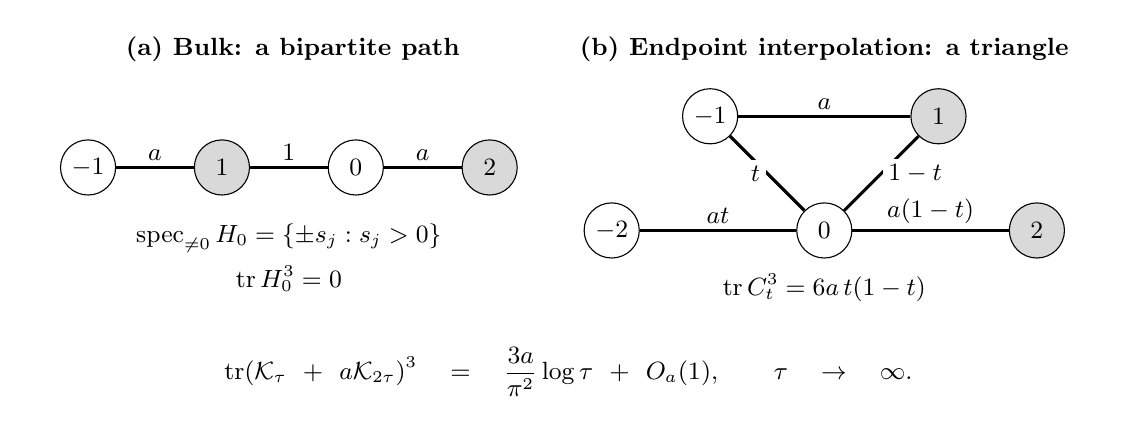
\begin{tikzpicture}[x=1cm,y=1cm,font=\small,
  vertex/.style={circle,draw,fill=white,minimum size=7mm,inner sep=0pt},
  positive/.style={vertex,fill=black!15},
  weight/.style={fill=white,inner sep=2pt}]
  \node[font=\small\bfseries] at (-3.50,1.50)
    {(a) Bulk: a bipartite path};
  \node[vertex] (bm) at (-6.10,0) {$-1$};
  \node[positive] (bp) at (-4.40,0) {$1$};
  \node[vertex] (bz) at (-2.70,0) {$0$};
  \node[positive] (bq) at (-1.00,0) {$2$};
  \draw[thick] (bm) -- node[weight,above] {$a$} (bp);
  \draw[thick] (bp) -- node[weight,above] {$1$} (bz);
  \draw[thick] (bz) -- node[weight,above] {$a$} (bq);
  \node[align=center] at (-3.55,-1.15)
    {$\operatorname{spec}_{\ne0}H_0=\{\pm s_j:s_j>0\}$\\[4pt]
     $\operatorname{tr}H_0^3=0$};
  \node[font=\small\bfseries] at (3.25,1.50)
    {(b) Endpoint interpolation: a triangle};
  \node[vertex] (cm) at (1.80,0.65) {$-1$};
  \node[positive] (cp) at (4.70,0.65) {$1$};
  \node[vertex] (cz) at (3.25,-0.80) {$0$};
  \node[vertex] (cl) at (0.55,-0.80) {$-2$};
  \node[positive] (cr) at (5.95,-0.80) {$2$};
  \draw[line width=1.1pt] (cm) -- node[weight,above] {$a$} (cp);
  \draw[line width=1.1pt] (cm) -- node[weight,left] {$t$} (cz);
  \draw[line width=1.1pt] (cp) -- node[weight,right] {$1-t$} (cz);
  \draw[thick] (cl) -- node[weight,above] {$at$} (cz);
  \draw[thick] (cz) -- node[weight,above] {$a(1-t)$} (cr);
  \node at (3.25,-1.53) {$\operatorname{tr}C_t^3=6a\,t(1-t)$};
  \node[align=center,text width=13.5cm] at (0,-2.60) {
    $\displaystyle
    \operatorname{tr}(\mathcal K_\tau+a\mathcal K_{2\tau})^3
       =\frac{3a}{\pi^2}\log\tau+O_a(1),\qquad \tau\to\infty.$};
\end{tikzpicture}
\caption{Exact weighted graphs for the two-harmonic family.
Vertices are Fourier indices; shaded vertices have positive index.
Isolated zero vertices are omitted in (a).
Every bulk edge joins the two index classes, so the bulk spectrum is
sign-symmetric. For $C_t=(1-t)H_0+tH_1$, the three edges on
$\{-1,0,1\}$ have product $a\,t(1-t)$.
The six oriented closed walks around this triangle give the cubic trace.
The logarithmic law also uses the polynomial localization and scalar
sawtooth calculation proved in the text. Here $a\in\mathbb R$ is fixed;
the triangle is present when $a\ne0$ and $0<t<1$.}
\label{fig:unified-two-harmonic}
\end{figure}

\endgroup
\section{Phase-dependent constant terms}\label{unified:sec:phase}
\begingroup
\let\section\subsection
\let\subsection\subsubsection
\section{Fixed-phase constant terms}\label{v11:sec:phase-constants}
Use the global exchange and full-fiber gauge of
Sections~\ref{sec:crosswindow} and~\ref{app:general-trace}, with scalar
star entries $c=c_\theta$, $s=s_\theta$. The block Toeplitz constant
\cite[Theorem~2.3 and Corollary~2.4]{BasorEhrhardtVirtanen2024}
combines with trace-norm \emph{convergence} of the physical boundary
corrections; boundedness alone does not give a constant term.

For $|z|<1$ put
\[
 \beta(z)=\varkappa\bigl(x\mapsto\log(1-zx)\bigr).
\]
The scalar logarithm and every determinant logarithm in this section are
analytic determinations equal to zero at $z=0$.

\begin{theorem}[Fixed-phase determinant and band-local trace constants]
\label{v11:thm:phase-constant}\label{v11:cor:band-constant}
For real $r,\phi$ there is a holomorphic function
$\mathfrak D(z;r,\phi)$ on $|z|<1$, with $\mathfrak D(0;r,\phi)=0$, such that
\begin{equation}\label{v11:eq:phase-det}
 \log\det(I-z\mathcal K_{n+r,\phi})
 =2(n+r)\log(1-z^2)+\beta(z)\log(n+r)
       +\mathfrak D(z;r,\phi)+o(1)
\end{equation}
as the integer $n$ tends to infinity.  The error is locally uniform in
$z$ and uniform for $(r,\phi)$ in a compact set.
For every real Lipschitz $f$ on $[-1,1]$ with $f(0)=0$ and $C^2$
restrictions to $[-1,-g]$ and $[g,1]$, where $g=2^{-1/2}$, there is a
continuous function $\mathfrak C_f(r,\phi)$ such that
\begin{equation}\label{v11:eq:phase-smooth}
 \operatorname{tr}f(\mathcal K_{n+r,\phi})
 =2(n+r)[f(1)+f(-1)]+\varkappa(f)\log(n+r)
       +\mathfrak C_f(r,\phi)+o(1),
\end{equation}
uniformly on compact sets of $(r,\phi)$. In particular, for every $p\ge1$,
\begin{equation}\label{v11:eq:schatten-constant}
 \|\mathcal K_{n+r,\phi}\|_p^p
 =4(n+r)+\varkappa_p\log(n+r)+\mathfrak C_p(r,\phi)+o(1).
\end{equation}
The determinant constant is specified by
\eqref{v11:eq:phase-constant-product}.
\end{theorem}

The diagonal identity
$\tr\mathcal K_{n+r,\phi}=2\pi^{-1}\sin(2\pi r)\cos\phi$
and locally uniform differentiation give
\begin{equation}\label{v11:eq:phase-first}
 \partial_z\mathfrak D(0;r,\phi)
 =-\frac2\pi\sin(2\pi r)\cos\phi.
\end{equation}
The second derivative is
\begin{equation}\label{v11:eq:phase-second}
 \partial_z^2\mathfrak D(0;r,\phi)=\frac2{\pi^2}
 [\log(4\pi)+1+\gamma_E+(\log2)\cos(4\pi r)\cos(2\phi)],
\end{equation}
where $\gamma_E$ is Euler's constant. Here is a direct check retaining
both phases. Write $s(u)=\sin(\pi u)/(\pi u)$ and let $C_\tau$ be
its compression to $(-\tau,\tau)$. Product-to-sum and the variables
$u=X-Y$, $v=X+Y$ give
\[
 \tr\mathcal K_{\tau,\phi}^2
 =2\tr C_\tau^2+\frac{2\cos(2\phi)}{\pi^3}
   \int_0^{2\tau}\frac{\sin^2(\pi u)\sin(4\pi\tau-2\pi u)}{u^2}du.
\]
Since $\int_\mathbb R s^2=1$,
\[
 2\tau-\tr C_\tau^2
 =4\tau\int_{2\tau}^\infty s(u)^2du+
       \frac2{\pi^2}\int_0^{2\tau}\frac{\sin^2(\pi u)}u du
 =\frac{1+\gamma_E+\log(4\pi\tau)}{\pi^2}+O(\tau^{-1}).
\]
The last equality follows by one integration by parts in the tail and
$\int_0^x(1-\cos t)dt/t=\gamma_E+\log x-\operatorname{Ci}(x)$,
where $\operatorname{Ci}(x)=-\int_x^\infty\cos t\,dt/t=O(x^{-1})$.
Extending the oscillatory integral to infinity costs $O(\tau^{-1})$.
The resulting cosine integral is zero, whereas
\[
 \int_0^\infty\frac{\sin^2(\pi u)\sin(2\pi u)}{u^2}du
 =\pi\int_0^\infty\frac{\cos(2\pi u)-\cos(4\pi u)}u du
 =\pi\log2.
\]
For the cosine integral use
$\sin^2(\pi u)\cos(2\pi u)=\tfrac12(\cos(2\pi u)-1)
-\tfrac14(\cos(4\pi u)-1)$ and
$\int_0^\infty(1-\cos au)du/u^2=\pi a/2$.
The sine identity follows by integration by parts and the damped
Frullani integral. Thus the quadratic trace is
$4\tau-2\pi^{-2}[\log(4\pi\tau)+1+\gamma_E+
(\log2)\cos(4\pi\tau)\cos(2\phi)]+O(\tau^{-1})$.
Twice differentiating the locally uniform limit
\eqref{v11:eq:phase-det} proves \eqref{v11:eq:phase-second}.

\subsection{Localization of the gauge correction}

Identify the physical space with
$\mathscr X=\ell^2(\mathbb Z;\mathscr H)$, where $\mathscr H=L^2(0,1)$,
and retain the symbols of Section~\ref{app:general-trace}.  Write
\[
 \mathscr B=\mathcal L(\sigma),\qquad
 \mathscr U=\mathcal L(V),\qquad
 \mathscr C=\mathscr U^*\mathscr B\mathscr U=\mathcal L(a).
\]
Thus $\mathscr B,\mathscr C$ are self-adjoint contractions and
$\mathscr U$ is unitary.  All three commute with the bilateral cell shift
$\mathsf S$, defined by $(\mathsf Sx)_j=x_{j-1}$.
Let $\Pi_+$ select the cells $j\ge0$, put $\Pi_-=I-\Pi_+$, and set
$R_m=\mathsf S^m\Pi_-\mathsf S^{-m}$.  The projection onto the cells
$0,\ldots,m-1$ satisfies
\begin{equation}\label{v11:eq:projection-split}
 P_m=\Pi_++R_m-I.
\end{equation}

Lemma~\ref{rev5:lem:seam} also gives $[\Pi_\pm,\mathscr U]\in\mathfrak S_1$
and the same for $\mathscr U^*$: each half-line has one inverse-square
Hankel corner and a Fourier remainder summable with weight $|k|$.

\begin{lemma}[Two boundary corrections]\label{v11:lem:gauge-localization}
For an orthogonal projection $E$ put
\[
 D(E)=\mathscr U^*E\mathscr B E\mathscr U-E\mathscr C E,
 \qquad D_+=D(\Pi_+),\quad D_-=D(\Pi_-).
\]
Then $D_+,D_-$ are trace class and
\begin{equation}\label{v11:eq:gauge-localization}
 \|D(P_m)-D_+-\mathsf S^mD_-\mathsf S^{-m}\|_1\longrightarrow0.
\end{equation}
\end{lemma}
\begin{proof}
The exact identity
\begin{equation}\label{v11:eq:D-identity}
 D(E)=\mathscr U^*E\mathscr B[E,\mathscr U]
             +[\mathscr U^*,E]\mathscr B\mathscr U E
\end{equation}
first proves the trace-class assertion.  Insert
\eqref{v11:eq:projection-split} in its two commutators and subtract the
identities for $\Pi_+$ and $R_m$.  The difference consists of exactly
\begin{align*}
 &\mathscr U^*(P_m-\Pi_+)\mathscr B[\Pi_+,\mathscr U],&
 &\mathscr U^*(P_m-R_m)\mathscr B[R_m,\mathscr U],\\
 &[\mathscr U^*,\Pi_+]\mathscr B\mathscr U(P_m-\Pi_+),&
 &[\mathscr U^*,R_m]\mathscr B\mathscr U(P_m-R_m).
\end{align*}
The first and third contain the strongly null projection
$P_m-\Pi_+=-\mathsf S^m\Pi_+\mathsf S^{-m}$. After translation by
$\mathsf S^{-m}$, the others contain $-\mathsf S^{-m}\Pi_-\mathsf S^m$.
Finite-rank approximation gives $\|X_mT\|_1\to0$ for fixed
$T\in\mathfrak S_1$ and uniformly bounded strongly null $X_m$;
it also gives $\|TX_m\|_1\to0$ when $X_m^*\to0$ strongly.
Applied to the fixed commutators, this proves all four limits.
\end{proof}

Set
\[
 \mathscr A_m=\mathscr U^*P_m\mathscr B P_m\mathscr U,
 \quad\mathscr C_m=P_m\mathscr C P_m,
 \quad\mathscr A_\pm=\mathscr U^*\Pi_\pm\mathscr B\Pi_\pm\mathscr U,
 \quad\mathscr C_\pm=\Pi_\pm\mathscr C\Pi_\pm.
\]
These are self-adjoint contractions; the finite compressions and
$D_\pm=\mathscr A_\pm-\mathscr C_\pm$ are trace class. Define
\begin{equation}\label{v11:eq:gauge-det-factors}
 e_\pm(z)=\det\bigl[I-zD_\pm(I-z\mathscr C_\pm)^{-1}\bigr],
 \qquad |z|<1.
\end{equation}
These determinants are holomorphic and nonzero, because their operators
equal $(I-z\mathscr A_\pm)(I-z\mathscr C_\pm)^{-1}$.

\begin{lemma}[Relative determinant convergence]\label{v11:lem:gauge-det}
Locally uniformly on $|z|<1$,
\begin{equation}\label{v11:eq:gauge-det-limit}
 \frac{\det(I-z\mathscr A_m)}{\det(I-z\mathscr C_m)}
       \longrightarrow e_+(z)e_-(z).
\end{equation}
The normalized analytic logarithms converge locally uniformly as well.
\end{lemma}
\begin{proof}
Let $X_\pm(z)=D_\pm(I-z\mathscr C_\pm)^{-1}$.
At each fixed boundary the reference resolvents and their adjoints
converge strongly, uniformly for $|z|\le\rho<1$, by the Neumann series
and its uniformly bounded tail. Lemma~\ref{v11:lem:gauge-localization}
and trace-class multiplication give
\[
 \left\|D(P_m)(I-z\mathscr C_m)^{-1}
       -X_+(z)-\mathsf S^mX_-(z)\mathsf S^{-m}\right\|_1\to0
\]
uniformly on each such disk.

Weakly null shifts and finite-rank approximation give
$\|T\mathsf S^mW\|_1\to0$ for trace-class $T,W$, uniformly on
trace-norm compact families by finite nets.
Consequently
\[
 (I-zX_+)(I-z\mathsf S^mX_-\mathsf S^{-m})
 =I-zX_+-z\mathsf S^mX_-\mathsf S^{-m}+o_{\mathfrak S_1}(1)
\]
uniformly on smaller disks.  Multiplicativity and trace-norm continuity
of the Fredholm determinant prove the limit, using the exact identity
\[
 I-z\mathscr A_m
 =\bigl[I-zD(P_m)(I-z\mathscr C_m)^{-1}\bigr](I-z\mathscr C_m).
\]
The nonzero limits equal one at zero; Cauchy differentiation and
integration of logarithmic derivatives give the normalized-log limit.
\end{proof}

\subsection{The model constant and fractional endpoints}

On $E=\operatorname{span}\{e_{-1},e_0,e_1\}$ put
$M_z(\theta)=I_E-za(\theta)$.  For real $|z|<1$, both $M_z$ and
$M_z^{-1}$ are uniformly positive definite.  Their half-line Toeplitz
operators are therefore invertible.  The symbol is piecewise smooth with
one jump, so Theorem~2.1 and Corollary~2.4 of
\cite{BasorEhrhardtVirtanen2024} apply.  In their notation,
\[
 L(z)=\frac1{2\pi i}
       \log[(I-zX_{1,0})^{-1}(I-zX_{0,-1})]
\]
has trace zero and its eigenvalues have real parts in $(-1/2,1/2)$.
Since $\det M_z\equiv1-z^2$, the cited result gives
\begin{equation}\label{v11:eq:model-strong}
 \det T_m(M_z)=(1-z^2)^m m^{\beta(z)}E_a(z)(1+o(1)),
 \qquad E_a(z)>0
\end{equation}
for real $|z|<1$.  Here $\beta(z)=-\operatorname{tr}L(z)^2$.
Its equality with the trace coefficient follows also by comparing
\eqref{v11:eq:model-strong}, Lemma~\ref{v11:lem:gauge-det}, and the
already established bounded-remainder law on the real interval.

The model constant has a specified Fredholm expression.  Let $T$ denote
the semi-infinite block Toeplitz operator, let $G_B$ be the Barnes
$G$-function, and set
\[
 u_z(\theta)=\exp\{i(2\pi\theta-\pi)L(z)\},\qquad0<\theta<1.
\]
If $\ell_1(z),\ell_2(z),\ell_3(z)$ are the unordered eigenvalues of
$L(z)$, the single-jump case of \cite[eq.~(2.11)]{BasorEhrhardtVirtanen2024}
reads
\begin{equation}\label{v11:eq:model-constant}
 E_a(z)=\prod_{j=1}^3G_B(1+\ell_j(z))G_B(1-\ell_j(z))
 \det\bigl[T(M_z)T(u_z)^{-1}T(u_z^{-1})^{-1}T(M_z^{-1})\bigr].
\end{equation}
The ordered product is identity plus trace class by that theorem; no
commutation of its factors is used.  The jump orientation agrees because
$u_z(0+)^{-1}u_z(1-)=M_z(0+)^{-1}M_z(1-)$.
The inverses of the single-jump factors follow from
\cite[Proposition~3.11]{BasorEhrhardtVirtanen2024}.

The cited applicability holds also for complex $|z|<1$.  Indeed
$\operatorname{Re}M_z\ge(1-|z|)I$ and
$\operatorname{Re}M_z^{-1}\ge(1-|z|)(1+|z|)^{-2}I$, so both required
Toeplitz operators are invertible by coercivity.  The endpoint ratio has
no negative real eigenvalue: otherwise a convex combination of its two
endpoint matrices would be singular, although that combination is
$I-z[(1-t)X_{1,0}+tX_{0,-1}]$.  Its principal matrix logarithm is thus
analytic, has trace zero by continuation from zero, and has the required
eigenvalue strip.

No parameter-uniform remainder is being inferred from the cited theorem.
For $|z|\le\rho<1$, the first two $x$ derivatives of $\log(1-zx)$ are
bounded by $\rho/(1-\rho)$ and $\rho^2/(1-\rho)^2$.  Apply the existing
uniform trace bound to its real and imaginary parts.  The normalized
physical logarithms are locally bounded holomorphic functions.  Their
convergence for real $z$, already supplied by
\eqref{v11:eq:model-strong} and Lemma~\ref{v11:lem:gauge-det}, extends
locally uniformly to the disk by Vitali's theorem.  This also gives the
normalized holomorphic determination of $\log E_a$.
Since $\mathcal K_n$ has $m=2n$ complete cells, its constant is
\begin{equation}\label{v11:eq:integer-constant}
 \mathfrak D_0(z)=\log E_a(z)+\beta(z)\log2
                   +\log e_+(z)+\log e_-(z).
\end{equation}

On the physical space let $L_b=P_{(b,\infty)}$ and
$H_b=P_{(-\infty,b)}$.  The two differences
\[
 F_b^L=L_b\mathcal G L_b-L_0\mathcal G L_0,
 \qquad F_b^R=H_b\mathcal G H_b-H_0\mathcal G H_0
\]
are trace class by Lemma~\ref{rev5:lem:strips}.  Define
\begin{align}
 d_L(z;b)&=\det\bigl[(I-zL_b\mathcal G L_b)
                             (I-zL_0\mathcal G L_0)^{-1}\bigr],\nonumber\\
 d_R(z;b)&=\det\bigl[(I-zH_b\mathcal G H_b)
                             (I-zH_0\mathcal G H_0)^{-1}\bigr].
 \label{v11:eq:endpoint-factors}
\end{align}
Each product is identity plus trace class and invertible for $|z|<1$.

For fixed $l,h$ let $E_m=P_{(l,m+h)}$ and $P_m=P_{(0,m)}$ in physical
coordinates.  Then
\begin{equation}\label{v11:eq:strip-localization}
 \|E_m\mathcal G E_m-P_m\mathcal G P_m
             -F_l^L-\mathsf S^mF_h^R\mathsf S^{-m}\|_1\to0.
\end{equation}
To check every term, set $\delta=L_l-L_0$ and
$\epsilon_m=\mathsf S^m(H_h-H_0)\mathsf S^{-m}$.
The identity $E_m=P_m+\delta+\epsilon_m$ holds once the interval is
nonempty.  After expanding and subtracting the two half-line
corrections, the remainder is
\begin{align*}
 &\delta\mathcal G(P_m-L_0)+(P_m-L_0)\mathcal G\delta\\
 &\quad+\epsilon_m\mathcal G(P_m-\mathsf S^mH_0\mathsf S^{-m})
       +(P_m-\mathsf S^mH_0\mathsf S^{-m})\mathcal G\epsilon_m\\
 &\quad+\delta\mathcal G\epsilon_m+\epsilon_m\mathcal G\delta.
\end{align*}
The first pair contains the escaping projection $-P_{(m,\infty)}$
and fixed trace-class strip products. Translating the second pair gives
the same argument at minus infinity. The last pair vanishes since
$\epsilon_m\to0$ strongly and $\delta\mathcal G,\mathcal G\delta$
are trace class. This proves \eqref{v11:eq:strip-localization}.
The proof of Lemma~\ref{v11:lem:gauge-det}, now with these boundary
corrections and the physical baseline resolvents, yields
\begin{equation}\label{v11:eq:endpoint-det-limit}
 \frac{\det(I-zE_m\mathcal G E_m)}{\det(I-zP_m\mathcal G P_m)}
       \longrightarrow d_L(z;l)d_R(z;h)
\end{equation}
locally uniformly in the disk.

For $a_0=\phi/(2\pi)$, dilation and integer translation identify
$\mathcal K_{n+r,\phi}$ with the compression to
$(a_0-r,2n+a_0+r)$.  Equations~\eqref{v11:eq:integer-constant}
and~\eqref{v11:eq:endpoint-det-limit} therefore specify the full constant:
\begin{equation}\label{v11:eq:phase-constant-product}
 \mathfrak D(z;r,\phi)=\mathfrak D_0(z)
     +\log d_L(z;\phi/(2\pi)-r)+\log d_R(z;\phi/(2\pi)+r)
     -2r\log(1-z^2).
\end{equation}
Replacing $\log n$ by $\log(n+r)$ costs $o(1)$, uniformly for bounded $r$.

The fixed-strip bound gives a length-independent trace-norm endpoint
modulus. For self-adjoint trace-class contractions, telescoping powers
in the logarithm series gives
\[
 |\log\det(I-zA)-\log\det(I-zB)|
       \le\frac\rho{1-\rho}\|A-B\|_1,
 \qquad |z|\le\rho<1.
\]
The limiting half-line factors are continuous in their endpoints in
trace norm.  Finite nets in a compact endpoint set upgrade the proved
convergence to uniform convergence there.

\begin{proof}[The $C^2$ trace case of Theorem~\ref{v11:thm:phase-constant}]
The determinant assertion has just been proved.  Differentiate its
locally uniform analytic limit at zero, using
\[
 \log\det(I-z\mathcal K)
       =-\sum_{k\ge1}\frac{z^k}{k}\operatorname{tr}\mathcal K^k.
\]
This proves convergence of the normalized trace remainder for every
polynomial vanishing at zero.  For $f\in C^2$, approximate $f''$
uniformly by polynomials and integrate twice with the exact values
$f(0)=0$ and $f'(0)$.  The approximants converge in $C^2$.
The uniform trace-remainder estimate of
Theorem~\ref{T10:conj:law} and Proposition~\ref{v6:prop:allphase}
makes their limiting constants Cauchy and transfers the limit to $f$,
uniformly on compact parameter sets.  It also proves continuity of the
limiting function.
\end{proof}

Uniqueness of the limit and the exact phase symmetries give
\begin{align*}
 \mathfrak D(z;r+1,\phi)&=\mathfrak D(z;r,\phi),&
 \mathfrak D(z;r,\phi+2\pi)&=\mathfrak D(z;r,\phi),\\
 \mathfrak D(z;r,-\phi)&=\mathfrak D(z;r,\phi),&
 \mathfrak D(z;r,\phi+\pi)&=\mathfrak D(-z;r,\phi).
\end{align*}
No elementary evaluation of the full Fredholm product, quantitative
rate for its remainder, or boundary value on a spectral cut is asserted.

\subsection{Lipschitz relative traces and Schatten constant terms}
\label{v11:sec:lip-constants}

The exact model gap permits a stronger conclusion than global $C^2$
regularity.  The needed relative-trace argument uses uniform finite-rank
approximation of the boundary corrections; it does not use an
operator-Lipschitz assertion.

\begin{lemma}[Finite-rank tightness of relative traces]
\label{v11:lem:lip-tightness}
Let $A_m,B_m$ be self-adjoint trace-class contractions.  Suppose
$\sup_m\|A_m-B_m\|_1<\infty$, and suppose that for every $\epsilon>0$
there are self-adjoint finite-rank operators $H_m$ such that, for all
sufficiently large $m$,
\[
 \operatorname{rank}H_m\le r_\epsilon,\qquad
 \|A_m-B_m-H_m\|_1\le\epsilon,
\]
where $r_\epsilon$ is independent of $m$.
If $\operatorname{tr}p(A_m)-\operatorname{tr}p(B_m)$ converges for every
polynomial $p$ with $p(0)=0$, then it converges for every real Lipschitz
$f$ on $[-1,1]$ with $f(0)=0$.
\end{lemma}
\begin{proof}
For a self-adjoint trace-class operator $A$, define the signed counting
function, with an immaterial value at zero, by
\[
 N_A(t)=\begin{cases}
 \#\{\lambda_j(A)>t\},&t>0,\\
 -\#\{\lambda_j(A)<t\},&t<0.
 \end{cases}
\]
It is integrable with $\int|N_A|=\|A\|_1$.  Absolute continuity of a
Lipschitz function and absolute summability of its scalar trace give
\begin{equation}\label{v11:eq:counting-trace}
 \operatorname{tr}f(A)=\int f'(t)N_A(t)\,dt.
\end{equation}
For $\xi_{A,B}=N_A-N_B$, two elementary bounds are
\begin{equation}\label{v11:eq:counting-shift-bounds}
 \int|\xi_{A,B}|\le\|A-B\|_1,
 \qquad
 |\xi_{A,B}(t)|\le\operatorname{rank}(A-B)\quad(t\ne0)
\end{equation}
when the rank is finite. Intersect a spectral subspace with
$\ker(A-B)$ and apply the variational characterization above a positive
threshold (or below a negative one) for the rank bound. For the integral
bound, decompose a finite-matrix difference into signed rank-one terms.
A positive increment has nonnegative counting difference by monotonicity,
with integral equal to its trace by \eqref{v11:eq:counting-trace}; reverse
negative increments and telescope. For trace-class operators, truncate
the two spectral expansions separately. Counts converge at every nonzero
threshold outside the two countable spectra; Fatou proves the bound.

Put $C_m=B_m+H_m$.  Its spectrum may extend outside $[-1,1]$, which
does not affect the estimates on that interval.  The exact identity
$\xi_{A_m,B_m}=\xi_{A_m,C_m}+\xi_{C_m,B_m}$ and
\eqref{v11:eq:counting-shift-bounds} imply, for bounded integrable $h$
supported in $[-1,1]$,
\begin{equation}\label{v11:eq:uniform-count-tightness}
 \left|\int h\xi_{A_m,B_m}\right|
 \le\epsilon\|h\|_\infty+r_\epsilon\|h\|_{L^1(-1,1)}.
\end{equation}
Uniform polynomial approximation of derivatives and
Lemma~\ref{rev5:lem:trace-lip} first extend convergence to $C^1$ tests.
For an $L$-Lipschitz $f$, mollify its zero-extended derivative and
integrate from zero. Then $f_\delta(0)=0$, $\|f_\delta'\|_\infty\le L$
and $\|f'-f_\delta'\|_1\to0$. Equations~\eqref{v11:eq:counting-trace}
and~\eqref{v11:eq:uniform-count-tightness} bound the relative-trace error by
\[
 2L\epsilon+r_\epsilon\|f'-f_\delta'\|_1.
\]
Choose $\epsilon$ first and then $\delta$. The bound is uniform for
large $m$, so convergence of the smooth relative traces makes the
original sequence Cauchy.
\end{proof}

Both comparisons in the preceding subsection satisfy this lemma.
Approximate $D_+,D_-$ by self-adjoint finite-rank $H_+,H_-$.
The sum $H_++\mathsf S^mH_-\mathsf S^{-m}$ has uniformly bounded rank
and approximates the gauge correction in trace norm. The same argument
applies to $F_l^L,F_h^R$. Polynomial relative traces converge by
locally uniform determinant differentiation, so the lemma supplies both
Lipschitz limits. These are limits of finite relative traces; no trace
of an infinite difference $f(A_\pm)-f(B_\pm)$ is assumed.

\begin{proof}[Band-local completion of Theorem~\ref{v11:thm:phase-constant}]
Choose $F\in C^2([-1,1])$ agreeing with $f$ on the two closed bands and
with $F(0)=0$.  For example, fill the central interval with the unique
polynomial of degree at most six matching the value and first two
derivatives at each of $-g,g$ and the value zero at zero.  These are the
seven Hermite conditions at nodes of multiplicities $3,1,3$.
Then $q=f-F$ is Lipschitz and vanishes at zero and on the two bands.

Lemma~\ref{v11:lem:model-gap} gives
exactly $m$ model eigenvalues in each band, and all other eigenvalues
are zero.  Thus $\operatorname{tr}q(T_m(a))=0$ exactly.  The Lipschitz
gauge comparison just established implies convergence of
$\operatorname{tr}q(\mathcal K_n)$.  Both its bulk and logarithmic
coefficients vanish, since the coefficient functional samples only the
two bands and their endpoints.  Add this limit to the global $C^2$
constant already proved for $F$.

The Lipschitz endpoint comparison gives the result for fixed $r,\phi$,
with bulk adjustment $2r[f(1)+f(-1)]$ and a vanishing change in the
logarithm.  The fixed-strip modulus and the scalar trace perturbation
bound give compact-parameter uniformity by finite nets.  Finally,
$|x|^p$ is Lipschitz for $p\ge1$ and is $C^2$ on both closed bands,
which proves \eqref{v11:eq:schatten-constant}.
\end{proof}

The band $C^2$ assumption in this theorem is stronger than the band
$C^{1,1}$ assumption sufficient for a bounded remainder in
Theorem~\ref{v7:thm:band-regularity}.  No convergent constant for that
entire larger class is inferred here.


\subsection{A phase constant for shrinking finite sampling scale}
Use the matrix of \eqref{eq:2.1} and the dimension-independent Lipschitz
comparison of Theorem~\ref{v11:thm:direct-transfer}, with
$\Gamma_\varepsilon=16\sqrt{2/\pi}\,\varepsilon/
[(1-2\varepsilon)\sqrt{1-4\varepsilon^2}]$.

\begin{corollary}[A third term for shrinking finite scale]
\label{v11:cor:finite-phase-constant}
Let $\varepsilon_N\to0$ and
$\tau_N=(2N+1)\varepsilon_N/2\to\infty$.  For every $f$ satisfying
Theorem~\ref{v11:cor:band-constant},
\begin{equation}\label{v11:eq:finite-phase-constant}
 \tr f(A_N(\varepsilon_N))
 =(2N+1)\varepsilon_N[f(1)+f(-1)]
  +\varkappa(f)\log\tau_N
  +\mathfrak C_f(\{\tau_N\},0)+o(1).
\end{equation}
Here $\{\tau_N\}$ is the fractional part, and the constant profile is
continuous and periodic.  This includes every Schatten power $p\ge1$,
with no condition on $(2N+1)\varepsilon_N^3$.
\end{corollary}
\begin{proof}
The direct Lipschitz comparison has error at most
$\Gamma_{\varepsilon_N}\operatorname{Lip}(f)=o(1)$.
Apply the phase law uniformly for $r\in[0,1]$ with
$n=\lfloor\tau_N\rfloor$ and $r=\{\tau_N\}$.
Periodicity follows from uniqueness under replacing $(n,r)$ by
$(n-1,r+1)$.  Thus convergence of the fractional parts is not required.
\end{proof}

For fixed $\varepsilon>0$ the comparison supplies a bounded remainder;
it does not identify a finite-matrix constant term in that regime.


\endgroup
\section{Physical gap states and one-period flow}\label{unified:sec:gap}
\begingroup
\let\section\subsection
\let\subsection\subsubsection
\section{Boundary spectra in the open central gaps}
\label{v11:sec:gap-limits}

Retain $\mathscr U,\mathscr C_\pm,L_b,H_b$ from
Section~\ref{v11:sec:phase-constants}. The same localization determines
every limiting eigenvalue away from zero and the band edges. Put
\[
 \Sigma=\{0\}\cup[-1,-g]\cup[g,1],\qquad
 \Omega=\mathbb C\setminus\Sigma,\qquad g=2^{-1/2}.
\]

\begin{lemma}[The reference resolvent gap]\label{v11:lem:model-gap}
The spectra of $\mathscr C_m,\mathscr C_+,\mathscr C_-$ are contained
in $\Sigma$.  The finite model has exactly $m$ positive and $m$ negative
eigenvalues.  Their resolvents, and the translated right resolvents,
converge strongly to the appropriate half-line resolvents, including
their adjoints, uniformly on compact subsets of $\Omega$.
\end{lemma}
\begin{proof}
For a finite or either half-infinite cell projection $E$, the scalar
compressions $C_E=E\mathcal L(c)E$ and $S_E=E\mathcal L(s)E$ satisfy
$C_E+S_E\ge I$ on that cell space because
$c(\theta)+s(\theta)\ge1$.  Hence
\[
 C_E^2+S_E^2
 =\tfrac12[(C_E+S_E)^2+(C_E-S_E)^2]\ge\tfrac12I.
\]
The row operator $B_E=(S_E,C_E)$ has $B_EB_E^*\ge I/2$ and is onto.
The polar decomposition of the star operator
$\left(\begin{smallmatrix}0&B_E\\B_E^*&0\end{smallmatrix}\right)$
therefore confines its nonzero spectrum to the two bands.  Its norm is
at most one by compression of $\mathcal L(a)$; the ambient complement
adds only zero.  The finite count follows from the row rank $m$.

At each fixed boundary the finite compressions converge strongly.
Continuous functional calculus on the common spectral set $\Sigma$
gives strong resolvent convergence. On compact $K\subset\Omega$ the
norm bound $\operatorname{dist}(K,\Sigma)^{-1}$, the resolvent identity
and finite nets give uniformity; conjugating the parameter handles
adjoints.
\end{proof}

For fixed real $l,h$ let $E_m=P_{(l,m+h)}$ in physical coordinates and
define
\[
 \mathscr A_m(l,h)=\mathscr U^*E_m\mathcal G E_m\mathscr U,
 \quad
 \mathscr A_l^+=\mathscr U^*L_l\mathcal G L_l\mathscr U,
 \quad
 \mathscr A_h^-=\mathscr U^*H_h\mathcal G H_h\mathscr U,
\]
\[
 D_l^+=\mathscr A_l^+-\mathscr C_+,
 \qquad D_h^-=\mathscr A_h^--\mathscr C_-.
\]
The last two differences are trace class.  Adding the gauge and strip
localizations gives
\begin{equation}\label{v11:eq:combined-gap-localization}
 \|\mathscr A_m(l,h)-\mathscr C_m-D_l^+
                  -\mathsf S^mD_h^-\mathsf S^{-m}\|_1\to0.
\end{equation}
Combining the corrections before taking the resolvent is essential:
the star baseline has a proved gap, whereas a physical half-line
baseline could itself have a gap eigenvalue.

Define, for $\lambda\in\Omega$,
\begin{align}
 F_m(\lambda;l,h)
   &=\det\bigl[I+(\mathscr A_m(l,h)-\mathscr C_m)
                             (\mathscr C_m-\lambda)^{-1}\bigr],\nonumber\\
 F_+(\lambda;l)
   &=\det\bigl[I+D_l^+(\mathscr C_+-\lambda)^{-1}\bigr],\qquad
 F_-(\lambda;h)
   =\det\bigl[I+D_h^-(\mathscr C_--\lambda)^{-1}\bigr].
 \label{v11:eq:gap-determinants}
\end{align}
They are analytic Fredholm determinants of identity plus trace-class
operators.  The signs follow from
$I+(A-C)(C-\lambda)^{-1}=(A-\lambda)(C-\lambda)^{-1}$.

\begin{theorem}[Local gap eigenvalue convergence]\label{v11:thm:gap-limits}
Locally uniformly on $\Omega$,
\begin{equation}\label{v11:eq:gap-det-limit}
 F_m(\lambda;l,h)\longrightarrow F_+(\lambda;l)F_-(\lambda;h).
\end{equation}
The two limiting factors have precisely the eigenvalues in $\Omega$
of $L_l\mathcal G L_l$ and $H_h\mathcal G H_h$ as zeros, respectively,
with their finite multiplicities.

For fixed $r,\phi$ take $l=\phi/(2\pi)-r$, $h=\phi/(2\pi)+r$ and
$m=2n$.  If $J$ is a compact interval strictly inside $(0,g)$ or
$(-g,0)$, with endpoints outside the two boundary spectra, then every
boundary eigenvalue $\alpha\in J$ attracts exactly
\begin{equation}\label{v11:eq:gap-multiplicity}
 k(\alpha)=\dim\ker(L_l\mathcal G L_l-\alpha)
             +\dim\ker(H_h\mathcal G H_h-\alpha)
\end{equation}
eigenvalues of $\mathcal K_{n+r,\phi}$, counting multiplicity.
For sufficiently large $n$ there are no other eigenvalues in $J$.
\end{theorem}
\begin{proof}
Use \eqref{v11:eq:combined-gap-localization} and
Lemma~\ref{v11:lem:model-gap} in the proof of
Lemma~\ref{v11:lem:gauge-det}.  Trace-class multiplication and the
vanishing product between shifted boundaries give
\eqref{v11:eq:gap-det-limit}, now locally uniformly on $\Omega$.

The limiting factors are relative determinants of the self-adjoint
half-line pairs. They are nonzero for nonreal $\lambda$, so analytic
Fredholm theory on the connected set $\Omega$ gives isolated zeros
with finite kernels. Conjugating by $\mathscr U$ identifies their
physical eigenspaces.

The zero order equals the eigenvalue multiplicity.  Indeed, for an
isolated eigenvalue $\alpha$ of multiplicity $k$, let $\Pi$ be its
finite-rank spectral projection and replace $A$ by
$\widetilde A=A+\epsilon\Pi$, moving that eigenvalue outside a small
disk.  Factor the relative determinant through $\widetilde A$.
Its nonvanishing analytic factor is multiplied by
\[
 \det[(A-\lambda)(\widetilde A-\lambda)^{-1}]
       =\left(\frac{\alpha-\lambda}{\alpha+\epsilon-\lambda}\right)^k.
\]
This also proves the multiplicity assertion for the finite determinants.

Around the finitely many limiting zeros in $J$, choose disjoint disks
in $\Omega$. Rouch\'e's theorem gives multiplicity
\eqref{v11:eq:gap-multiplicity} in each for large $m$; all finite zeros
are real. The limit is bounded away from zero on the remaining compact
set, excluding other roots. Shrinking the disks proves convergence.
\end{proof}

\subsection{Exact eventual count offsets}

For $\lambda\in(0,g)$ outside the two boundary spectra, define
\begin{align}
 \iota_+(\lambda;l)
  &=\operatorname{tr}\bigl[\mathbf1_{(\lambda,\infty)}(\mathscr A_l^+)
                  -\mathbf1_{(\lambda,\infty)}(\mathscr C_+)\bigr],\nonumber\\
 \iota_-(\lambda;h)
  &=\operatorname{tr}\bigl[\mathbf1_{(\lambda,\infty)}(\mathscr A_h^-)
                  -\mathbf1_{(\lambda,\infty)}(\mathscr C_-)\bigr].
 \label{v11:eq:gap-indices}
\end{align}
The differences are trace class: integrate the trace-class resolvent
differences over a positively oriented rectangle enclosing
$[\lambda,1]$, whose left side crosses the real axis at $\lambda$ and
whose right side lies beyond one.  Each trace is an integer.  To see
this directly for a trace-class difference $D=P-Q$ of orthogonal
projections, note that $D$ anticommutes with $P+Q-I$ and
$(P+Q-I)^2=I-D^2$.  Thus its eigenvalues in $(-1,1)\setminus\{0\}$
pair with their negatives.  Only the finite-dimensional $+1$ and $-1$
eigenspaces contribute to its trace.

\begin{corollary}[Fixed-threshold counts inside the gap]
\label{v11:cor:gap-count-offset}
With $l,h$ as in Theorem~\ref{v11:thm:gap-limits}, for every
$\lambda\in(0,g)$ outside the boundary spectra one has, for all
sufficiently large integers $n$,
\begin{equation}\label{v11:eq:exact-gap-count}
 \#\{\lambda_j(\mathcal K_{n+r,\phi})>\lambda\}
       =2n+\iota_+(\lambda;l)+\iota_-(\lambda;h).
\end{equation}
The analogous formula for $\lambda\in(-g,0)$ counts eigenvalues below
$\lambda$, with the negative spectral projections and the same
reference count $2n$.
\end{corollary}
\begin{proof}
On the contour just described the limiting determinant is nonzero.
Equation~\eqref{v11:eq:gap-det-limit} and Cauchy differentiation imply
convergence of the logarithmic derivatives there.  Direct differentiation
of the relative determinant, followed by the resolvent identity, gives
\[
 \frac{F_m'(\zeta)}{F_m(\zeta)}
 =\operatorname{tr}\bigl[(\zeta-\mathscr A_m)^{-1}
                              -(\zeta-\mathscr C_m)^{-1}\bigr],
\]
and the same identity holds for each half-line factor.
Contour integration consequently gives
\[
 \#\{\lambda_j(\mathscr A_m)>\lambda\}-m
       \longrightarrow\iota_+(\lambda;l)+\iota_-(\lambda;h).
\]
Both sides are integers, so equality holds eventually.  The reference
count is exactly $m$ by Lemma~\ref{v11:lem:model-gap}, and $m=2n$.
For the negative version use a contour enclosing $[-1,\lambda]$.
\end{proof}

\subsection{The two parity copies for a centered interval}

\begin{corollary}[Parity of an isolated gap cluster]
\label{v11:cor:gap-parity}
For $\phi=0$, let $\alpha$ be an isolated eigenvalue in either open
central gap of $L_{-r}\mathcal G L_{-r}$, of multiplicity $k$.
Exactly $k$ eigenvalues in each parity sector of $\mathcal K_{n+r}$
converge to $\alpha$.  The statement for $\phi=\pi$ follows by negating
the eigenvalues.
\end{corollary}
\begin{proof}
Reflection exchanges $L_{-r}\mathcal G L_{-r}$ and
$H_r\mathcal G H_r$, giving total multiplicity $2k$.
On $(-r,2n+r)$ the reflection $\mathcal R_nu(X)=u(2n-X)$ commutes
with the physical compression; no gauge symmetry is needed.

Let $v_1,\ldots,v_k$ be an orthonormal basis of the left half-line
eigenspace, extended by zero, and put $v_{j,n}=E_{2n}v_j$.
Strong convergence gives $v_{j,n}\to v_j$ and
\[
 \|(E_{2n}\mathcal G E_{2n}-\alpha)v_{j,n}\|\to0.
\]
Reflection preserves residual norms and is weakly null as its center
escapes, so left/right inner products tend to zero. Each family
\[
 2^{-1/2}(v_{j,n}+\mathcal R_nv_{j,n}),\qquad
 2^{-1/2}(v_{j,n}-\mathcal R_nv_{j,n}),\qquad1\le j\le k,
\]
has Gram matrix tending to identity and residual tending uniformly to
zero on its span. The spectral theorem forces at least $k$ nearby
eigenvalues in each parity. The exact total $2k$ makes both counts
$k$; shrinking the neighborhood proves convergence.
\end{proof}

\subsection{One boundary phase for each gap value}
\label{boundary:sec:one-cell-flow}

Write $B_b=L_b\mathcal G L_b|_{L^2(b,\infty)}$.  For
$\sigma\in\{1,-1\}$, $0<t<g$, and $\sigma t\notin\operatorname{spec}B_b$,
put
\[
 I_\sigma(t;b)=\operatorname{tr}\bigl[
 \mathbf1_{(t,\infty)}(\sigma\mathscr A_b^+)
 -\mathbf1_{(t,\infty)}(\sigma\mathscr C_+)\bigr].
\]
Thus $I_+(t;b)=\iota_+(t;b)$, whereas $I_-$ counts negative eigenvalues
of the left boundary operator by their magnitude.
The one-period count is analogous to the Dirichlet spectral flow for
periodic Hill operators \cite[Proposition~3.21]{Gontier2020}.
Here the projection index and analytic bandlimited covariance provide
the crossing count for the nonlocal sine-Loewner compression.

\begin{theorem}[One-cell boundary spectral flow]
\label{boundary:thm:one-cell-flow}
At regular thresholds $I_\sigma(t;b)$ is nonincreasing in $b$, and
\begin{equation}\label{boundary:eq:index-period}
 I_\sigma(t;b+1)=I_\sigma(t;b)-1.
\end{equation}
For every $\lambda\in(-g,0)\cup(0,g)$, precisely one phase
$b\pmod1$ has $\lambda\in\operatorname{spec}B_b$, and this eigenvalue
is simple.  Every local gap eigenbranch is real analytic and satisfies
\begin{equation}\label{boundary:eq:hadamard}
 \lambda'(b)=-\lambda(b)|u_b(b)|^2
\end{equation}
for a normalized physical eigenfunction $u_b$.  Its magnitude is
strictly decreasing along a connected gap branch; the derivative is
allowed to vanish at isolated phases.
\end{theorem}

\begin{proof}
For $b<c$, $\delta=c-b$, and $E=P_{(b,c)}$, one has
\[
 L_b\mathcal G L_b-L_c\mathcal G L_c
 =E\mathcal G L_b+L_c\mathcal G E.
\]
The Taylor expansion of the restricted Fourier kernel about $b$ gives
\[
 \|E\mathcal F^*\mathbf1_{(-1,1)}\|_1
 \le\sum_{n\ge0}\frac{(2\pi)^n}{n!}
 \|(x-b)^n\|_{L^2(b,c)}\|\xi^n\|_{L^2(-1,1)}
 \le\sqrt{2\delta}\,e^{2\pi\delta}.
\]
Thus $\mathcal G=\mathcal F^*J\mathcal F$ gives trace-norm modulus
$2\sqrt{2\delta}e^{2\pi\delta}$. At a regular threshold a common
Riesz contour makes the relative projection continuous in trace norm,
and its integer trace locally constant.

For monotonicity work in physical space and put
$P_b=\mathbf1_{(t,\infty)}(\sigma L_b\mathcal G L_b)$.
For $b<c$ and $0\ne u\in\operatorname{ran}P_c$,
\[
 \langle u,\sigma L_b\mathcal G L_bu\rangle
 =\langle u,\sigma L_c\mathcal G L_cu\rangle>t\|u\|^2.
\]
Hence $\operatorname{ran}P_c\cap\ker P_b=\{0\}$.  The trace formula
for a trace-class difference of projections yields
$\operatorname{tr}(P_b-P_c)
=\dim(\operatorname{ran}P_b\cap\ker P_c)\ge0$.

Let $Q_\sigma=\mathbf1_{(t,\infty)}(\sigma\mathscr C_+)$.
We next show
\begin{equation}\label{boundary:eq:reference-one-cell}
 \operatorname{tr}(Q_\sigma-\mathsf S Q_\sigma\mathsf S^{-1})=1.
\end{equation}
Deform the star row to a constant by
$c_a=(1-a)c+a$, $s_a=(1-a)s$, $0\le a\le1$.
Then $c_a+s_a\ge1$ and $(c_a^2+s_a^2)^{1/2}\le1$.
The proof of Lemma~\ref{v11:lem:model-gap} therefore preserves the
gap throughout this homotopy.  The difference of a half-line star
and its one-cell translate is finite rank, continuously in trace norm:
only the rows and columns of the removed cell in the fixed
three-dimensional star fiber occur.  A resolvent contour shows that
$Q_{\sigma,a}-\mathsf S Q_{\sigma,a}\mathsf S^{-1}$ is trace-class
continuous.  Its integer trace is constant.  At $a=1$ the constant
star has one state of each sign per cell, so the trace is one.
Since the gauge commutes with the cell shift and $G(x+1,y+1)=G(x,y)$,
$\mathscr A_{b+1}^+=\mathsf S\mathscr A_b^+\mathsf S^{-1}$.
Equation~\eqref{boundary:eq:reference-one-cell} now proves
\eqref{boundary:eq:index-period}.

We exclude a nonzero gap eigenvalue persisting on a phase interval.
On $\mathcal H=L^2(-1,1)$ let $V_b$ be Fourier synthesis restricted
to $(b,\infty)$ and set $Q_b=V_b^*V_b$.  Then
\[
 B_b=V_bJV_b^*,\qquad
 \mathcal T_b(\lambda)=Q_b-\lambda J.
\]
For $\lambda\ne0$, the $I-AB$/$I-BA$ block factorization makes
$B_b-\lambda$ invertible, respectively Fredholm, if and only if
$\mathcal T_b(\lambda)$ is.  Their kernels have the same dimension:
if $\mathcal T_b(\lambda)u=0$, then $V_bu\ne0$ and
$B_bV_bu=\lambda V_bu$; conversely $B_bf=\lambda f$ gives the
nonzero kernel vector $JV_b^*f$.
With $v_x(\xi)=e^{2\pi ix\xi}$,
\begin{equation}\label{boundary:eq:covariance-rank-one}
 Q_b-Q_c=\int_b^c|v_x\rangle\langle v_x|\,dx,
 \qquad Q_b'=-|v_b\rangle\langle v_b|.
\end{equation}
The integral is in trace norm.  The bounded frequency interval makes
$Q_b$ norm analytic, and the pencil is self-adjoint Fredholm at a real
nonzero central-gap parameter.

If a fixed $\lambda$ persisted on an interval, analytic spectral
reduction, after avoiding any isolated extra crossings, would give
a nonzero analytic kernel bundle of constant finite rank.
Choose an orthonormal parallel frame $u_j(b)$, so that its derivative
has zero projection onto the kernel.  Differentiating
$\mathcal T_b(\lambda)u_j(b)=0$ gives
\[
 0=\langle u_j,Q_b'u_j\rangle
 =-|\langle v_b,u_j\rangle|^2.
\]
Thus $Q_b'u_j=0$, the differentiated equation puts $u_j'$ in the
kernel, and parallel transport forces $u_j'=0$.
The Fourier transform of this constant nonzero vector would vanish
on an interval.  Its bounded frequency support makes it entire,
a contradiction.  Analytic Fredholm reduction now shows that the
crossing phases for a fixed $\lambda$ are isolated and therefore
finite in a period.

For the crossing direction, translate the half-line to $(0,\infty)$.
The kernel $G_b(x,y)=G(x+b,y+b)$ is a norm-analytic sine/cosine
combination of two fixed bounded operators.  Isolated eigenclusters
have real-analytic eigenbranches.  A nonzero eigenfunction is the
restriction of $\lambda^{-1}\mathcal G_b\widetilde u$, a bandlimited
function, so all its boundary traces exist and it belongs to
$H^k(0,\infty)$ for every $k$.  Integration by parts, using
$\partial_bG_b=\partial_xG_b+\partial_yG_b$, gives
\[
 B_b'u=(\lambda-B_b)\partial_xu-G_b(\cdot,0)u(0).
\]
The boundary eigenvalue equation and Hellmann--Feynman identity imply
\eqref{boundary:eq:hadamard}.  Each magnitude branch is therefore
nonincreasing.  It cannot be constant on any interval by the preceding
argument, so it is strictly decreasing in value.  The derivative can
have isolated zeros.

Choose a regular phase $b_0$ for a fixed $\sigma t$.
At a crossing of multiplicity $k$, isolate the finite cluster between
two nearby regular thresholds.  Its $k$ analytic branches all cross
downward in magnitude, and local constancy at the lower threshold
shows that $I_\sigma(t;b)$ drops by $k$.  Its total drop on
$(b_0,b_0+1)$ is one.  Hence
\[
 \sum_{b\in(b_0,b_0+1):\,\sigma t\in\operatorname{spec}B_b}
 \dim\ker(B_b-\sigma t)=1.
\]
This proves both the unique crossing phase and simplicity.
\end{proof}

\begin{corollary}[Opposite signs and centered clusters]
\label{boundary:cor:opposite-signs}
For $0<t<g$, the unique phases at which $t$ and $-t$ occur differ
by $1/2$ modulo one.  In particular, no $B_b$ has both $t$ and $-t$
as eigenvalues.  Every isolated gap cluster in the centered case of
Corollary~\ref{v11:cor:gap-parity} consists of exactly one even and one
odd eigenvalue for all sufficiently large $n$.
\end{corollary}
\begin{proof}
Translation by $1/2$ changes $G$ to $-G$, so
$B_{b+1/2}$ is unitarily equivalent to $-B_b$.
Uniqueness of the crossing phase proves the first two claims.
Theorem~\ref{boundary:thm:one-cell-flow} makes the multiplicity $k$ in
Corollary~\ref{v11:cor:gap-parity} equal to one.
\end{proof}

The flow does not evaluate the crossing phase or an absolute index,
identify a floor-ranked level, or control limits toward zero or the band
edges. Infinitely many levels accumulating at zero remain possible.

\begin{figure}[htbp]
\centering
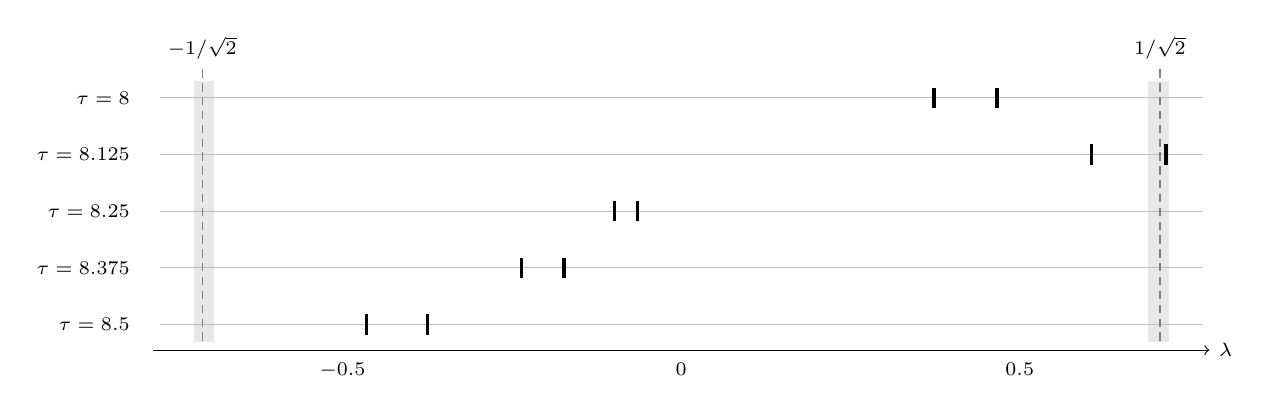
\begin{tikzpicture}[x=8.6cm,y=0.72cm]
  \fill[black!9] (0.69,0.3) rectangle (0.72,-4.3);
  \fill[black!9] (-0.72,0.3) rectangle (-0.69,-4.3);
  \foreach \y/\t/\a/\b in {0/8/0.373543/0.466256,-1/8.125/0.605497/0.716075,-2/8.25/-0.098190/-0.064436,-3/8.375/-0.236090/-0.172944,-4/8.5/-0.464887/-0.374640} {
    \draw[gray!50] (-0.77,\y) -- (0.77,\y);
    \node[font=\scriptsize,anchor=east] at (-0.8,\y) {$\tau=\t$};
    \draw[very thick] (\a,{\y-0.18}) -- (\a,{\y+0.18});
    \draw[very thick] (\b,{\y-0.18}) -- (\b,{\y+0.18});
  }
  \draw[densely dashed,gray] (0.707107,0.5) -- (0.707107,-4.3);
  \draw[densely dashed,gray] (-0.707107,0.5) -- (-0.707107,-4.3);
  \node[font=\scriptsize,anchor=south] at (0.707107,0.5) {$1/\sqrt2$};
  \node[font=\scriptsize,anchor=south] at (-0.707107,0.5) {$-1/\sqrt2$};
  \foreach \x in {-0.5,0,0.5}
    \node[font=\scriptsize,anchor=north] at (\x,-4.5) {$\x$};
  \draw[->] (-0.78,-4.45) -- (0.78,-4.45) node[right,font=\scriptsize] {$\lambda$};
\end{tikzpicture}
\caption{Fractional-scale dependence: each row shows all eigenvalues with
$0.05<|\lambda|<0.72$; shading marks $0.69<|\lambda|<0.72$.
The selection is not a continuation of fixed branches: the last three
scales also have a positive eigenvalue outside the window, at $0.7478$,
$0.7836$ and $0.7860$. Thus neither displayed signs nor guard-band
emptiness is uniform in $\tau$. Gauss--Legendre and Clenshaw--Curtis
values agree to $10^{-10}$; these are ordinary-precision samples from
\texttt{anc/verify\_phase\_dependence.py}, not certified boundary limits.}
\label{fig:phase-dependence}
\end{figure}


\section{An explicit endpoint equation and quantitative gap limits}
\label{v12:sec:boundary-mellin}

We make the limiting spectral equation explicit and derive the physical
tail exponent. Unlike the adjacent-interval transform diagonalized in
\cite[Sections~2--4]{BertolaEtAl2020}, this pencil retains same-interval
Hilbert blocks and a phased exchange, producing four endpoint channels.

For $\theta=2\pi l$, define on $L^2(-1,1)$
\[
 Q_0=\tfrac12(I+iH),\qquad
 Hu(\xi)=\frac1\pi\operatorname{pv}\int_{-1}^1
                   \frac{u(\eta)}{\xi-\eta}\,d\eta,
\]
\[
 (J_\theta u)(\xi)=
 \begin{cases}e^{-i\theta}u(\xi-1),&0<\xi<1,\\
 e^{i\theta}u(\xi+1),&-1<\xi<0,
 \end{cases}
 \qquad P_\lambda=Q_0-\lambda J_\theta.
\]

\begin{proposition}[Exact frequency pencil]\label{v12:prop:frequency-pencil}
For every nonzero $\lambda$, the physical operator $L_l\mathcal G L_l$
has eigenvalue $\lambda$ precisely when $P_\lambda$ has a nonzero kernel.
The correspondence preserves the algebraic multiplicity of an isolated
eigenvalue.  If $P_\lambda u=0$, its physical eigenfunction is the
restriction to $X>l$ of
\begin{equation}\label{v12:eq:physical-continuation}
 h(X)=\int_{-1}^1e^{-2\pi i(X-l)\xi}u(\xi)\,d\xi,
 \qquad \mathcal G L_lh=\lambda h\quad\hbox{on }\mathbb R.
\end{equation}
Equivalently, the frequency equation is
$Hu=i(I-2\lambda J_\theta)u$.
\end{proposition}
\begin{proof}
Let $V_l$ restrict inverse Fourier transformation from $L^2(-1,1)$ to
$L^2(l,\infty)$, and let $M_lu(\xi)=e^{2\pi il\xi}u(\xi)$.
Direct integration gives $L_l\mathcal G L_l=V_lJV_l^*$ and
$V_l^*V_l=M_lQ_0M_l^*$, where $J=J_0$.
The bounded-product identity used in
Theorem~\ref{boundary:thm:one-cell-flow} preserves nonzero spectra
and isolated algebraic multiplicities. Conjugation by $M_l$ gives
$J_\theta Q_0$ and $P_\lambda$. The map $V_lM_l$ is injective by
entire uniqueness. Finally $Q_0u=\lambda J_\theta u$ implies
$JV_l^*V_lM_lu=\lambda M_lu$; inverse transformation on the whole line
gives \eqref{v12:eq:physical-continuation}.
\end{proof}

The endpoint channels are $u(t),u(t-1),u(1-t),u(-t)$ as $t\downarrow0$.
For real Mellin frequency $\omega$, put
\[
 q=\frac{1+\tanh\pi\omega}{2},\qquad
 r=\frac{1-\tanh\pi\omega}{2},\qquad
 c=\tfrac12\operatorname{sech}\pi\omega,
 \qquad D_\theta=\operatorname{diag}(1,e^{i\theta},e^{-i\theta},1).
\]
The endpoint pencil has the explicit multiplier
\begin{equation}\label{v12:eq:endpoint-symbol}
 m_{\lambda,\theta}(\omega)=D_\theta
 \begin{pmatrix}
 q&-\lambda&0&ic\\-\lambda&q&0&0\\
 0&0&r&-\lambda\\-ic&0&-\lambda&r
 \end{pmatrix}D_\theta^*,\qquad
 \det m_{\lambda,\theta}
 =\lambda^2\left(\lambda^2-\frac{1+\tanh^2\pi\omega}{2}\right).
\end{equation}
Its inverse is its adjugate divided by the displayed scalar determinant.
In particular it is a bounded Mellin multiplier for $\lambda\in\Omega$.

For $K\in\mathfrak S_2$ we use the regularized determinant
$\det_2(I+K)=\det((I+K)e^{-K})$; the operator inside the latter
determinant differs from the identity by a trace-class operator
\cite[Chapter~9]{Simon2005}.

\begin{theorem}[Explicit scalar equation in the central gaps]
\label{v12:thm:explicit-gap-equation}
The cutoff construction in Section~\ref{v12:app:mellin-proofs} gives
explicit operators $E,\mathcal I,M_\lambda,N_\lambda,\Delta_e,\Delta_i$, where
$M_\lambda^{-1}$ has symbol $m_{\lambda,\theta}^{-1}$ from
\eqref{v12:eq:endpoint-symbol}, $N_\lambda^{-1}$ is a piecewise constant
Fourier multiplier, and $\Delta_e,\Delta_i$ have the elementary
Hilbert--Schmidt kernels \eqref{v12:eq:endpoint-defect-kernel} and
\eqref{v12:eq:interior-defect-kernel}.  Define
\begin{align}
 R_\lambda&=E^*M_\lambda^{-2}E+\mathcal I^*N_\lambda^{-2}\mathcal I,\nonumber\\
 K_\lambda&=E^*(M_\lambda^{-2}\Delta_eP_\lambda
                          +M_\lambda^{-1}\Delta_e)
          +\mathcal I^*(N_\lambda^{-2}\Delta_iP_\lambda
                          +N_\lambda^{-1}\Delta_i).
 \label{v12:eq:explicit-preconditioner}
\end{align}
Then $R_\lambda P_\lambda^2=I+K_\lambda$, with $K_\lambda$ holomorphic
in $\mathfrak S_2$ on $\Omega$.  For every real
$\lambda\in(-g,0)\cup(0,g)$,
\begin{equation}\label{v12:eq:scalar-quantization}
 \det{}_2(I+K_\lambda)=0
 \quad\Longleftrightarrow\quad
 \lambda\in\sigma_p(L_l\mathcal G L_l).
\end{equation}
An eigenvalue of multiplicity $k$ is a zero of order $2k$.
Here $R_\lambda\ge(1+|\lambda|)^{-2}I$ on the real gaps; it remains
invertible on a neighborhood of each such point.  No global complex
invertibility of $R_\lambda$ is asserted.
\end{theorem}

\begin{theorem}[Endpoint exponent and physical tails]
\label{v12:thm:boundary-tail}
Let $\lambda\in(-g,0)\cup(0,g)$ and
$u\in\ker P_\lambda\setminus\{0\}$, and define
\begin{equation}\label{v12:eq:gap-exponent}
 \beta(\lambda)=\frac1\pi\arctan\sqrt{1-2\lambda^2},\qquad
 \nu=\tfrac12+\beta,\qquad
 \gamma(\lambda)=2\beta
 =\frac1\pi\arccos\frac{\lambda^2}{1-\lambda^2}.
\end{equation}
There is a possibly zero vector $v=(v_1,v_2,v_3,v_4)^T$ in the
one-dimensional kernel of $m_{\lambda,\theta}(-i\beta)$ such that, for
every fixed $\beta<a<1/2$,
\begin{equation}\label{v12:eq:endpoint-expansion}
 (u(t),u(t-1),u(1-t),u(-t))^T
       =t^{\nu-1}v+O(t^{-1/2+a}).
\end{equation}
The expansion holds after any fixed number of derivatives, with the
corresponding power lost from the remainder.  The continuation in
\eqref{v12:eq:physical-continuation}, with $\sigma=\operatorname{sgn}T$,
satisfies
\begin{align}
 h(l+T)=\frac{\Gamma(\nu)}{(2\pi|T|)^\nu}
 \big[&e^{-i\sigma\pi\nu/2}(v_1+e^{2\pi iT}v_2)
       +e^{i\sigma\pi\nu/2}(v_4+e^{-2\pi iT}v_3)\big]
       +O(|T|^{-1/2-a}).
 \label{v12:eq:physical-tail}
\end{align}
In particular, $|h(l+T)|\le C(1+|T|)^{-\nu}$.  More precisely,
\begin{equation}\label{v12:eq:tail-mass}
 \int_L^\infty|h(l+\sigma T)|^2\,dT
   =C_\sigma L^{-\gamma(\lambda)}+O(L^{-\beta-a}),
\end{equation}
where
\[
 C_\sigma=\frac{\Gamma(\nu)^2}{(2\pi)^{2\nu}(2\beta)}
 \left(|e^{-i\sigma\pi\nu/2}v_1+e^{i\sigma\pi\nu/2}v_4|^2
                            +|v_2|^2+|v_3|^2\right).
\]
Both constants are positive if $v\ne0$.  Their vanishing is not excluded.
\end{theorem}

\begin{corollary}[Rate for each isolated boundary cluster]
\label{v12:cor:gap-cluster-rate}
Fix $l,h$ and an isolated eigenvalue $\alpha$ in either open central gap
of one or both boundary operators in Theorem~\ref{v11:thm:gap-limits}.
Let $k$ be its total boundary multiplicity.  For integer $m\to\infty$,
the $k$ eigenvalues of $P_{(l,m+h)}\mathcal G P_{(l,m+h)}$ converging
to $\alpha$ satisfy
\[
 \max_{1\le j\le k}|\lambda_j-\alpha|
       =O(m^{-\gamma(\alpha)}).
\]
The constants may depend on the fixed endpoints, eigenvalue, and
separating interval.  In the centered case, each of the two parity
clusters in Corollary~\ref{v11:cor:gap-parity} obeys this rate.
\end{corollary}

Section~\ref{v12:app:mellin-proofs} proves the claims and supplies a
finite-rank error scheme. The equation does not evaluate its roots in
closed form; the tail and rate apply to every isolated root.

\section{Proofs of the endpoint equation and gap rate}
\label{v12:app:mellin-proofs}

\subsection{The explicit local models and all localization errors}

In coordinates $f_1(t)=u(t)$, $f_2(t)=u(t-1)$, $0<t<1$, the finite
Hilbert transform has kernel
\[
 \frac1\pi\begin{pmatrix}
 \operatorname{pv}(t-s)^{-1}&(t-s+1)^{-1}\\
 (t-s-1)^{-1}&\operatorname{pv}(t-s)^{-1}
 \end{pmatrix}.
\]
On $L^2(0,\infty)$ let $H_\infty,C_\infty$ have kernels
$[\pi(t-s)]^{-1}$, in principal value, and $[\pi(t+s)]^{-1}$.
On four copies of this space set
\[
 H_e=\begin{pmatrix}
 H_\infty&0&0&C_\infty\\0&H_\infty&0&0\\
 0&0&-H_\infty&0\\-C_\infty&0&0&-H_\infty
 \end{pmatrix},\quad Q_e=\tfrac12(I+iH_e),\quad
 J_e=\operatorname{diag}(J_\theta,J_\theta),\quad
 M_\lambda=Q_e-\lambda J_e.
\]
For the unitary Mellin transform
$\mathcal Mf(\omega)=(2\pi)^{-1/2}\int_0^\infty
t^{-1/2-i\omega}f(t)\,dt$, the two scalar multipliers are
$-i\tanh\pi\omega$ and $\operatorname{sech}\pi\omega$.
Indeed these follow from the principal-value cotangent integral and
the beta integral at exponent $1/2+i\omega$.  Thus $M_\lambda$ has
multiplier \eqref{v12:eq:endpoint-symbol}.  Expansion of its determinant
gives $\lambda^4-\lambda^2(q^2+r^2)+q^2r^2-c^2qr$; using $c^2=qr$
proves the asserted formula.  The $2\times2$ block of $Q_e$ on
channels 1 and 4 is a projection, and its other entries are $q,r$.
Consequently $0\le Q_e\le I$.  The inverse multiplier is bounded on
compact subsets of $\Omega$: its denominator is bounded away from zero,
and its adjugate is bounded.

Choose $0<\delta<1/4$ and a real smooth cutoff $0\le\chi\le1$, equal to one on
$[0,\delta]$ and zero on $[2\delta,\infty)$, such that
$\psi(t)=\sqrt{1-\chi(t)^2-\chi(1-t)^2}$ is smooth.  A smooth
sine/cosine transition has this property.  Extend $\psi$ by zero.
Define
\[
 Ef(t)=\chi(t)(f_1(t),f_2(t),f_1(1-t),f_2(1-t))^T,
 \qquad \mathcal If=\psi f,
\]
where the outputs are in $L^2((0,\infty);\mathbb C^4)$ and
$L^2(\mathbb R;\mathbb C^2)$, respectively, with zero extension.
Their adjoints are
\[
 E^*v(t)=\begin{pmatrix}
 \chi(t)v_1(t)+\chi(1-t)v_3(1-t)\\
 \chi(t)v_2(t)+\chi(1-t)v_4(1-t)
 \end{pmatrix},\qquad \mathcal I^*w(t)=\psi(t)w(t).
\]
Hence $E^*E+\mathcal I^*\mathcal I=1$, $EJ_\theta=J_eE$, and $\mathcal IJ_\theta=J_\theta\mathcal I$.
Let $Q_i$ be the whole-line Cauchy projection on each of the two interior
components and $N_\lambda=Q_i-\lambda J_\theta$.  In angular Fourier
frequency,
\begin{equation}\label{v12:eq:interior-inverse}
 n_\lambda(\omega)^{-1}=
 \begin{cases}-\lambda^{-1}J_\theta,&\omega<0,\\
 (I+\lambda J_\theta)/(1-\lambda^2),&\omega>0.
 \end{cases}
\end{equation}

The errors $\Delta_e=EQ_0-Q_eE$ and $\Delta_i=\mathcal IQ_0-Q_i\mathcal I$ are
independent of $\lambda,\theta$.  For $t>0$, $0<s<1$, the first has
kernel
\begin{equation}\label{v12:eq:endpoint-defect-kernel}
 \frac{i}{2\pi}\begin{pmatrix}
 \dfrac{\chi(t)-\chi(s)}{t-s}&
 \dfrac{\chi(t)-\chi(1-s)}{t+1-s}\\[5pt]
 \dfrac{\chi(t)}{t-1-s}&
 \dfrac{\chi(t)-\chi(s)}{t-s}\\[5pt]
 \dfrac{\chi(t)-\chi(1-s)}{1-t-s}&
 \dfrac{\chi(t)}{2-t-s}\\[5pt]
 -\dfrac{\chi(t)-\chi(s)}{t+s}&
 \dfrac{\chi(t)-\chi(1-s)}{1-t-s}
 \end{pmatrix}.
\end{equation}
For $t\in\mathbb R$, $0<s<1$, the second has kernel
\begin{equation}\label{v12:eq:interior-defect-kernel}
 \frac{i}{2\pi}\begin{pmatrix}
 (\psi(t)-\psi(s))/(t-s)&\psi(t)/(t-s+1)\\
 \psi(t)/(t-s-1)&(\psi(t)-\psi(s))/(t-s)
 \end{pmatrix}.
\end{equation}
Divided differences take their continuous values; a term supported where
its numerator is identically zero is zero.  The kernels are square integrable: diagonal quotients are bounded by
cutoff derivatives; corner quotients vanish below distance $\delta$,
with denominator at least $\delta$ elsewhere; unmatched cross terms
are separated from their poles. Output tails are $O(|t|^{-1})$.
The touching-endpoint Carleman singularity remains in the model.

\subsection{The scalar equation and its multiplicities}

\begin{proof}[Proof of Theorem~\ref{v12:thm:explicit-gap-equation}]
The intertwining errors satisfy
$EP_\lambda=M_\lambda E+\Delta_e$ and
$\mathcal IP_\lambda=N_\lambda\mathcal I+\Delta_i$.  Therefore
\[
 EP_\lambda^2=M_\lambda^2E+M_\lambda\Delta_e+\Delta_eP_\lambda,
\]
with the analogous interior identity.  Multiplying by the inverse
squares and using $E^*E+\mathcal I^*\mathcal I=1$ gives
\eqref{v12:eq:explicit-preconditioner}.  All inverse powers here are
algebraic powers, not adjoint products.  The explicit multipliers are
bounded and holomorphic on $\Omega$, so $K_\lambda$ is holomorphic in
$\mathfrak S_2$.

For real gap $\lambda$, self-adjoint model pencils of norm at most
$1+|\lambda|$ have inverse squares at least $(1+|\lambda|)^{-2}I$.
Thus $R_\lambda$ is invertible and $P_\lambda^2$ is Fredholm, with
$\ker P_\lambda^2=\ker P_\lambda$. The exact frequency correspondence
proves the real zero equivalence.

At a real isolated eigenvalue $\alpha$ of multiplicity $k$, the
bounded-product correspondence identifies the nonzero generalized
eigenspace of $J_\theta Q_0$ with that of the self-adjoint physical
operator.  It is therefore semisimple of dimension $k$.  Its Riesz
decomposition splits $J_\theta Q_0-\lambda$ into
$(\alpha-\lambda)I_k$ and an invertible analytic complement.  The
analytic Fredholm pencil $P_\lambda=J_\theta(J_\theta Q_0-\lambda)$
has characteristic multiplicity $k$; its square has multiplicity $2k$.
Multiplication by the locally invertible analytic $R_\lambda$ preserves
this number.  Finite-dimensional Schur reduction of an identity plus
$\mathfrak S_2$ family shows that its regularized determinant has this
zero order; the regularizing factor is a nonvanishing exponential.
\end{proof}

The equation permits finite-rank error control.  For $T\ge2$, the
displayed kernels give
\[
 \|\mathbf1_{t>T}\Delta_e\|_2^2\le\frac3{2\pi^2(T-1)},\qquad
 \|\mathbf1_{|t|>T}\Delta_i\|_2^2\le\frac1{\pi^2(T-1)}.
\]
There are six nonzero endpoint tail entries, bounded by
$(2\pi)^{-1}(t-1)^{-1}$, and two diagonal interior entries on each tail.
On the remaining finite rectangles, midpoint step approximations with
mesh widths $h_t,h_s$ have Hilbert--Schmidt error at most
$\sqrt T(B_th_t+B_sh_s)/2$, or
$\sqrt{2T}(B_th_t+B_sh_s)/2$ for the interior, where $B_t,B_s$ bound
the Frobenius norms of the two kernel derivatives.  Such bounds follow
from cutoff second derivatives and the canceled corner formulas.
The squared rectangle and tail errors add.

Replacing only the errors in \eqref{v12:eq:explicit-preconditioner}
by these finite-rank approximations gives, for example,
\[
 \|K_e-K_{e,n}\|_2\le
 (\|M_\lambda^{-1}\|^2(1+|\lambda|)+\|M_\lambda^{-1}\|)
                    \|\Delta_e-\Delta_{e,n}\|_2.
\]
Every multiplier is explicit; matrix evaluation errors must also be
controlled in a certificate.  A contour may certify zeros only when
it bounds a domain $D$ with $\overline D\Subset\Omega$ and
$R_\lambda$ proved invertible throughout $\overline D$.  If model
inverse norms are at most $b$ on a disk about real $\lambda_0$, then
$\|R_\lambda-R_{\lambda_0}\|\le2b^3|\lambda-\lambda_0|$; a disk with
$2b^3|\lambda-\lambda_0|<(1+|\lambda_0|)^{-2}$ suffices.
On the contour, a verified bound
$\|(I+K_{\lambda,n})^{-1}\|\,\|K_\lambda-K_{\lambda,n}\|<1$
keeps the interpolation invertible.  Half the finite determinant winding
then counts physical eigenvalues with multiplicity.  No such numerical
enclosure is claimed by the construction alone.

\subsection{Endpoint expansions and physical tails}

\begin{proof}[Proof of Theorem~\ref{v12:thm:boundary-tail}]
For $P_\lambda u=0$, set $f=-\Delta_eu$.  The displayed kernel implies,
for every integer $j\ge0$,
\[
 |f^{(j)}(t)|\le C_j\|u\|_2\quad(0\le t\le2),\qquad
 |f^{(j)}(t)|\le C_j\|u\|_2t^{-1-j}\quad(t\ge2).
\]
On bounded rectangles, derivatives of divided differences are bounded
by cutoff derivatives; corner cancellation and separated denominators
handle the other entries.  At infinity one differentiates rational
tails.  These are estimates on kernels applied to $u\in L^2$, so no
regularity of $u$ has been assumed.  Consequently
$\widehat f=\mathcal Mf$ is holomorphic in
$|\operatorname{Im}\omega|<1/2$ and rapidly decreases horizontally on
every closed smaller strip: in logarithmic coordinates,
$e^{x/2}f(e^x)$ and all its derivatives decay exponentially at both
ends, allowing repeated integration by parts.

Since $M_\lambda Eu=f$, Mellin inversion gives
\[
 Eu(t)=\frac1{\sqrt{2\pi}}\int_{\mathbb R}
 t^{-1/2+i\omega}m_{\lambda,\theta}(\omega)^{-1}
                     \widehat f(\omega)\,d\omega.
\]
The determinant in \eqref{v12:eq:endpoint-symbol} has exactly two simple
zeros in this strip, at $\pm i\beta$.  Away from these poles the inverse has bounded horizontal limits.
Shifting down to $\operatorname{Im}\omega=-a$ crosses only $-i\beta$, giving
\[
 v=-i\sqrt{2\pi}\operatorname*{Res}_{\omega=-i\beta}
                  (m_{\lambda,\theta}^{-1}\widehat f).
\]
The remaining integral is $O(t^{-1/2+a})$ and may be differentiated
any fixed number of times.  Since $\chi=1$ near zero, this proves
\eqref{v12:eq:endpoint-expansion}.  A simple determinant zero has matrix
rank three, so the residue lies in the stated one-dimensional kernel;
it may vanish.

The interior error has smooth derivatives and rational tails.
From $N_\lambda\mathcal Iu=-\Delta_i u$ and
\eqref{v12:eq:interior-inverse}, the Fourier transform of $\mathcal Iu$
decays rapidly at high frequency and is locally $L^2$ at zero.
Thus $u$ is smooth away from its three endpoints.

A cutoff of $t^{\nu-1}$ at zero has Fourier asymptotic
$\Gamma(\nu)e^{-i\operatorname{sgn}(T)\pi\nu/2}
(2\pi|T|)^{-\nu}+O(|T|^{-1})$, by the regularized Gamma integral.
A remainder $r(t)=O(t^{\mu-1})$, $r'(t)=O(t^{\mu-2})$, $0<\mu<1$,
has Fourier transform $O(|T|^{-\mu})$: split at $|T|^{-1}$ and integrate
the upper part by parts.  Applying these formulas to the four endpoints
with $\mu=1/2+a$ gives \eqref{v12:eq:physical-tail}, with the phases
$e^{2\pi iT}$ and $e^{-2\pi iT}$ from endpoints $-1$ and $1$.

After squaring, the nonoscillating part integrates to
$L^{1-2\nu}/(2\nu-1)$; nonzero integer-frequency cross terms are
$O(L^{-2\nu})$ by integration by parts.  The remainder cross term is
$O(L^{1-\nu-\mu})=O(L^{-\beta-a})$, proving
\eqref{v12:eq:tail-mass}.  At $\omega=-i\beta$, the kernel equations
and $|q|=|r|=c=\sqrt{(1-\lambda^2)/2}$ give
\[
 |v_4|=|v_1|,\qquad
 |v_2|=|v_3|=
          \frac{\sqrt2|\lambda|}{\sqrt{1-\lambda^2}}|v_1|.
\]
Thus a nonzero residue makes both tail constants strictly positive,
even if the zero-frequency amplitude cancels.
\end{proof}

\begin{proof}[Proof of Corollary~\ref{v12:cor:gap-cluster-rate}]
Theorem~\ref{v13:thm:leading-interaction}, proved independently from the
boundary tails and the qualitative gap limit, gives the stronger
$\lambda_j=\alpha+L^{-\gamma(\alpha)}\mu_j+o(L^{-\gamma(\alpha)})$
for both boundaries and $\lambda=\alpha+o(L^{-\gamma(\alpha)})$
for one boundary. Since $L=m+h-l$, these imply the stated rate,
including each centered parity sector.
\end{proof}


The following two structural results clarify the endpoint analysis: the scalar Hilbert model has an exact spectral measure, whereas the physical kernel admits no smooth scalar second-order formal commutant.
\section{Exact endpoint spectral measure}\label{eshort:sec}
Let $T$ be the finite Hilbert transform on $(-1,1)$,
$Tf(x)=\pi^{-1}\operatorname{p.v.}\int_{-1}^1 f(y)/(x-y)\,dy$,
and put $\Pi_T=(I-iT)/2$. Thus $T^*=-T$, $\|T\|\le1$, and
$\Pi_T$ is a positive contraction. Its classical spectral representation
\cite{KoppelmanPincus1959} gives the following exact endpoint law.

\begin{proposition}[Endpoint spectral measure]\label{T10:prop:lump}
For every $u>0$, $g_u(x)=[\pi(1+u-x)]^{-1}$ has normalized
$iT$-spectral measure $\tfrac12\mathbf1_{[-1,1]}(y)dy$. In particular,
\begin{equation}\label{eshort:moments}
 \|g_u\|^2=\frac2{\pi^2u(2+u)},\qquad
 \|T^kg_u\|^2=\frac{\|g_u\|^2}{2k+1},\qquad
 \langle g_u,\Pi_T^a g_u\rangle=\frac{\|g_u\|^2}{a+1}
 \quad(k\ge0,\ a\ge0),
\end{equation}
where $k$ is an integer.
\end{proposition}
\begin{proof}
The unitary Cayley map $\mathcal Wf(s)=\sqrt2 f((1-s)/(1+s))/(1+s)$
gives $\mathcal WT\mathcal W^*=-H_+$, where
$H_+F(s)=\pi^{-1}\operatorname{p.v.}\int_0^\infty F(t)/(s-t)dt$.
Indeed $x(s)-x(t)=2(t-s)/[(1+s)(1+t)]$. Also
$\mathcal Wg_u=\sqrt2\phi_w/(2+u)$, with
$w=u/(2+u)$ and $\phi_w(s)=[\pi(w+s)]^{-1}$.
For $\mathfrak MF(\omega)=\int_0^\infty F(s)s^{-1/2+i\omega}ds$,
Parseval has factor $(2\pi)^{-1}$, and
\begin{equation}\label{eshort:mellin}
 \mathfrak M\phi_w=w^{-1/2+i\omega}\operatorname{sech}(\pi\omega),
 \qquad \mathfrak MH_+\mathfrak M^{-1}=i\tanh(\pi\omega).
\end{equation}
These follow from the beta integral
$\int_0^\infty r^{z-1}/(1+r)dr=\pi/\sin\pi z$ and
$\operatorname{p.v.}\int_0^\infty r^{z-1}/(1-r)dr=\pi\cot\pi z$,
$0<\Re z<1$. For the latter, split at one and invert the upper part;
the geometric series gives
$\sum_{n\ge0}[(n+z)^{-1}-(n+1-z)^{-1}]=\pi\cot\pi z$.
Substituting $s=tr$ in the transformed Hilbert kernel gives the
multiplier $-\cot(\pi/2+i\pi\omega)=i\tanh(\pi\omega)$.
Regulated compactly supported calculations extend by boundedness to
$L^2$. Since $\|\phi_w\|^2=1/(\pi^2w)$, its normalized density is
$(\pi/2)\operatorname{sech}^2(\pi\omega)d\omega$; setting
$y=\tanh(\pi\omega)$ gives $dy/2$. Integrating $y^{2k}$ and
$((1-y)/2)^a$ proves the claims.
\end{proof}

\begin{corollary}[Endpoint leakage]\label{T10:cor:leak}
For the zero extension of $g_u$ and the whole-line Hilbert transform $H$,
\begin{equation}\label{eshort:leak}
 \int_{-1}^1|Hg_u|^2=\tfrac13\|g_u\|^2,\qquad
 \int_{|x|>1}|Hg_u|^2=\tfrac23\|g_u\|^2.
\end{equation}
\end{corollary}
\begin{proof}
Inside the interval $Hg_u=Tg_u$; apply \eqref{eshort:moments} with
$k=1$ and the whole-line $L^2$ isometry. Partial fractions also give
$Hg_u(x)=[\pi^2(1+u-x)]^{-1}\log[u|1+x|/((2+u)|1-x|)]$,
with the removable value at $x=1+u$ understood by continuity.
\end{proof}


\section{A scalar differential commutator obstruction}
\label{boundary:app:commutator}

The scalar second-order differential route available for several
classical Hankel kernels does not apply to the present physical
half-line kernel.  The following obstruction is an interior identity;
it is independent of endpoint-domain choices.

\begin{proposition}[No smooth scalar second-order formal commutant]
\label{boundary:prop:no-second-order}
Let $I=(a,\infty)$, $p\in C^1(I)$, $q\in C(I)$, and
$\mathcal L u=-(pu')'+qu$.  If
\[
 (\mathcal L_x-\mathcal L_y)
 \frac{\sin x-\sin y}{x-y}=0
 \qquad(x,y\in I,\ x\ne y),
\]
then $p=0$ and $q$ is constant.  The coefficients may be complex.
\end{proposition}
\begin{proof}
Put $d=x-y$ and $\Delta=\sin x-\sin y$.  Direct differentiation gives
\begin{align*}
 d^3(\mathcal L_x-\mathcal L_y)\frac{\Delta}{d}
 ={}&d^2[p(x)\sin x+p(y)\sin y-p'(x)\cos x-p'(y)\cos y]\\
 &+2d[p(x)\cos x-p(y)\cos y]\\
 &+\{d^2[q(x)-q(y)]+d[p'(x)+p'(y)]-2[p(x)-p(y)]\}\Delta.
\end{align*}
Choose $s=\pi/2+n\pi>a+\pi$ and set $x=s+t$, $y=s-t$,
$|t|<s-a$.  Then $\Delta=0$.  With
$P_s(t)=p(s+t)+p(s-t)$, the displayed identity reduces to
\[
 \sin t\,P_s'(t)+(\cos t-\sin t/t)P_s(t)=0,
 \qquad
 \left(\frac{\sin t}{t}P_s(t)\right)'=0.
\]
The second equation extends through zero by continuity.  Its constant
is $2p(s)$, while evaluation at $t=\pi$ makes that constant zero.
Thus $p$ is odd about every such center $s$.
For any $x>a$, choose $s$ sufficiently large and compose reflection
about $s$ with reflection about $s+\pi$.  Both reflected points stay
in $I$, and the two sign changes give $p(x+2\pi)=p(x)$.
The same periodicity holds for $p'$.

Now take $y=x+2\pi$ in the original differentiated identity.
It gives $p(x)\sin x-p'(x)\cos x=0$, or $(p(x)\cos x)'=0$.
The constant vanishes at a zero of cosine, so $p=0$ everywhere by
continuity.  The remaining equation is
$(q(x)-q(y))(\sin x-\sin y)=0$.  It makes $q$ constant; when two
sine values coincide, use a third point with a different sine value.
\end{proof}

The unitary change $x=2\pi X$ turns the physical kernel into a constant
multiple of the displayed one.  A commuting realization whose identity
includes compactly supported smooth test functions must satisfy this
formal interior equation, by integration by parts.  The proposition
excludes that smooth scalar second-order class.  It does not exclude
higher-order, matrix, nonlocal, or interior-singular differential models.

\begin{corollary}[Polynomial expressions on a finite interval]
\label{T10:prop:nocommute}
Let $\tau>0$, $D=d/dx$, and $p,q,s$ be real polynomials. If
$L=DpD+q+\tfrac i2(sD+Ds)$ satisfies
\begin{equation}\label{eshort:commute}
 (L^x-\overline L^{\,y})K_\tau(x,y)=0\qquad(-1<x,y<1),
\end{equation}
then $p=s=0$ and $q$ is constant.
\end{corollary}
\begin{proof}
The real part of the identity analytically continues to all real
$x,y$: the divided difference has removable diagonal and is entire.
Rescale by $2\pi\tau$ and apply Proposition~\ref{boundary:prop:no-second-order}
on a half-line, with the sign of $p$ reversed, to obtain $p=0$ and
constant $q$. The imaginary part on the diagonal is
$(s(x)\cos(2\pi\tau x))'=0$. Its constant vanishes at the zeros of
cosine, so $s=0$.
\end{proof}



\endgroup
\section{Algebraic interaction of the boundaries}\label{unified:sec:interaction}
\begingroup
\let\section\subsection
\let\subsection\subsubsection
\section{The leading interaction of the two boundaries}
\label{v13:sec:boundary-interaction}

We evaluate the full interaction, including the complementary-space
correction, which has the same order as the direct coupling. The
reduction is analogous to Feshbach--Schur
\cite[Theorem~1.2 and equations~(1.15)--(1.16)]{DussonSigalStamm2021};
the physical sine-Loewner modes determine its explicit coefficient.

Fix a real $\alpha\in(-g,0)\cup(0,g)$, and write
\begin{equation}\label{v13:eq:interaction-parameters}
 a=\sqrt{1-2\alpha^2},\qquad
 \beta=\pi^{-1}\arctan a,\qquad \nu=\tfrac12+\beta,\qquad
 \gamma=2\beta,\qquad
 c_\alpha=-\frac{\pi a(1+a^2)}{\alpha}.
\end{equation}
For a normalized left boundary eigenfunction $\psi_L$ on $(l,\infty)$,
define its physical tail amplitude by
\begin{equation}\label{v13:eq:physical-amplitude}
 \eta_L=\lim_{T\to\infty}T^\nu
                 \int_T^{T+1}\psi_L(l+x)\,dx
 =\frac{\Gamma(\nu)}{(2\pi)^\nu}
       \left(e^{-i\pi\nu/2}v_1+e^{i\pi\nu/2}v_4\right),
\end{equation}
where $v$ is the endpoint vector in
Theorem~\ref{v12:thm:boundary-tail}, scaled so that its physical
eigenfunction has norm one on the half-line.  The limit follows from
\eqref{v12:eq:physical-tail}: integration over one unit interval
removes the two nonzero leading carrier frequencies.  For a normalized
right boundary eigenfunction $\psi_R$ on $(-\infty,h)$, define
$\eta_R$ by the same limit with $\psi_R(h-x)$ in the integrand.
The amplitudes may vanish; their phase follows the eigenfunction's phase.
The same amplitude is determined in modulus by the normalized physical
tail mass:
\[
 \lim_{T\to\infty}T^\gamma\int_T^\infty
       |\psi_L(l+x)|^2\,dx=\frac{|\eta_L|^2}{\alpha^2\gamma}.
\]
Indeed the tail direction in the proof has squared norm $\alpha^{-2}$;
the nonmatching carriers integrate to a lower order. The right analogue
holds with $\psi_R(h-x)$.

\begin{theorem}[Closed leading boundary interaction]
\label{v13:thm:leading-interaction}
Fix $l,h$, and suppose that $\alpha$ is an isolated eigenvalue of one
or both half-line operators in Theorem~\ref{v11:thm:gap-limits}.
Their individual eigenvalues are simple by
Theorem~\ref{boundary:thm:one-cell-flow}.  Set
\[
 T_m=P_{(l,m+h)}\mathcal G P_{(l,m+h)},\qquad L=m+h-l,
 \qquad m\longrightarrow\infty\quad(m\in\mathbb Z).
\]
If $\alpha$ belongs to both boundary spectra, let $\mu_1\le\mu_2$
be the eigenvalues of the Hermitian matrix
\begin{equation}\label{v13:eq:closed-interaction-matrix}
 \mathsf M_\alpha=c_\alpha
 \begin{pmatrix}0&\overline{\eta_L}\eta_R\\
                 \overline{\eta_R}\eta_L&0\end{pmatrix}.
\end{equation}
The two finite-interval eigenvalues converging to $\alpha$, in
increasing order within the cluster, satisfy
\begin{equation}\label{v13:eq:leading-cluster-law}
 \lambda_j(T_m)=\alpha+L^{-\gamma}\mu_j+o(L^{-\gamma}),
 \qquad j=1,2.
\end{equation}
If $\alpha$ belongs to only one boundary spectrum, its single
eigenvalue satisfies $\lambda(T_m)=\alpha+o(L^{-\gamma})$.
All parameters are fixed; no uniformity as $\alpha$ approaches zero
or a band edge is asserted.
\end{theorem}

The two-boundary case implies $l+h\in\mathbb Z$.
Indeed reflection identifies the right operator at $h$ with the left
operator at $-h$, and Theorem~\ref{boundary:thm:one-cell-flow}
assigns a fixed nonzero gap level to a unique boundary phase modulo one.
Conversely, this congruence makes the two half-line operators unitarily
equivalent. Centered intervals satisfy the congruence automatically.

\begin{corollary}[Centered parity splitting]
\label{v13:cor:leading-parity-splitting}
Let $\alpha$ be an isolated eigenvalue of $L_{-r}\mathcal G L_{-r}$,
with normalized eigenfunction of amplitude $\eta$ in
\eqref{v13:eq:physical-amplitude}.  For the centered operator
$\mathcal K_{n+r}$, put $L=2(n+r)$.  Its unique even and odd
eigenvalues converging to $\alpha$ satisfy
\begin{align}
 \lambda_{\rm even}
   &=\alpha+c_\alpha|\eta|^2L^{-\gamma}+o(L^{-\gamma}),\nonumber\\
 \lambda_{\rm odd}
   &=\alpha-c_\alpha|\eta|^2L^{-\gamma}+o(L^{-\gamma}).
 \label{v13:eq:closed-parity-law}
\end{align}
Their midpoint is $\alpha+o(L^{-\gamma})$.  If $\eta\ne0$, their
splitting has the nonzero leading magnitude
$2|c_\alpha||\eta|^2L^{-\gamma}$, and eventually
$|\lambda_{\rm even}|<|\lambda_{\rm odd}|$.
If $\eta=0$, both shifts are $o(L^{-\gamma})$; strict ordering is
not inferred.  In fact both shifts are $O(L^{-1+\delta})$ for every
fixed $\delta>0$ in this case.
\end{corollary}

Section~\ref{v13:app:boundary-interaction} proves the full correction
and evaluates its scalar integral. Theorem~\ref{boundary:thm:certified-residue:rr}
certifies $\eta\ne0$ for the phase-zero mode.


\section{Proof of the leading boundary interaction}
\label{v13:app:boundary-interaction}

Throughout, $\alpha$ is real and lies in an open central gap, and
$\beta,\nu,\gamma,a$ are as in
\eqref{v13:eq:interaction-parameters}.  Put $\epsilon=L^{-\gamma}$.
Inner products are conjugate linear in the first variable.

\subsection{The physical tail directions}

Put $t=\pi\beta$, $q=(1-ia)/2$, $\overline q=(1+ia)/2$, and
$c=(2\cos t)^{-1}$.  These are the endpoint multiplier values at
$\omega=-i\beta$, so that $q=ce^{-it}$, $\overline q=ce^{it}$, and
$q^2+\overline q^{\,2}=\alpha^2$.  Undoing $D_\theta$ in
\eqref{v12:eq:endpoint-symbol}, the kernel vector with first
component one is
\[
 (1,(\alpha/c)e^{it},-i(\alpha/c)e^{2it},-ie^{3it})^T.
\]
The second and third rows give $v_2=\alpha v_1/q$ and
$v_3=\alpha v_4/\overline q$; the first gives
$v_4=i(q^2-\alpha^2)/(cq)=-i\overline q^{\,2}/(cq)$, and the fourth then holds.
If the first component is zero all four are zero.

Use global physical carriers in the order $(-1,0,1)$, and put
\[
 \mathsf A=\begin{pmatrix}0&1&0\\1&0&1\\0&1&0\end{pmatrix},
 \qquad
 \mathsf S=\begin{pmatrix}0&1&0\\1&0&-1\\0&-1&0\end{pmatrix},
\qquad v_+=\begin{pmatrix}\overline q/\alpha\\1\\q/\alpha\end{pmatrix},
 \quad v_-=\overline{v_+}.
\]
Let $A^\pm$ be the tail vectors of the full continuation of the
normalized left mode, and $B^\pm$ those of the right mode, with the
superscript denoting the direction $X\to\pm\infty$.  Thus, for example,
\[
 \widetilde\psi_L(X)=|X-l|^{-\nu}
       \sum_{p=-1}^1 A_p^\pm e^{2\pi ipX}+O(|X-l|^{-\mu}),
 \qquad \nu<\mu<1.
\]
Substitution in \eqref{v12:eq:physical-tail} gives
\begin{equation}\label{v13:eq:universal-tail-vectors}
 A^+=\eta_Lv_+,\qquad A^-=-i(c/\alpha)\mathsf SA^+,
 \qquad B^-=\eta_Rv_-,\qquad B^+=i(c/\alpha)\mathsf SB^-.
\end{equation}
Here the factors of $D_\theta$ cancel the factors from replacing
$e^{2\pi ip(X-l)}$ by $e^{2\pi ipX}$.  To check the ratios explicitly,
put $\varphi=\pi/4+t/2$.  The positive-tail vector before its common
Gamma factor is
$(e^{i\varphi}v_3,e^{-i\varphi}v_1+e^{i\varphi}v_4,
e^{-i\varphi}v_2)$; its middle component is
$2\cos(2t)e^{-i\pi/4+3it/2}$.  Division by it gives
$(\overline q/\alpha,1,q/\alpha)$.  Reversing the Gamma phases gives the
second formula in \eqref{v13:eq:universal-tail-vectors}; reflection
gives the two right formulas.  Since $\cos(2t)>0$, $\eta_L$ vanishes
precisely when the endpoint vector vanishes, and likewise on the right.

\subsection{The three-channel limit and residual profiles}

Let $H_{\mathbb R}$ have kernel $[\pi(s-t)]^{-1}$, set
$P_\pm=(I\pm iH_{\mathbb R})/2$, and define
\[
 \mathbb G=\begin{pmatrix}0&P_+&0\\P_+&0&P_-\\0&P_-&0\end{pmatrix},
 \qquad
 (\mathcal U_Lf)(X)=L^{-1/2}\sum_{p=-1}^1
              e^{2\pi ipX}f_p((X-l)/L).
\]
These maps have norm at most $\sqrt3$ and, for fixed $f,g\in L^2(\mathbb R)^3$, satisfy
\begin{equation}\label{v13:eq:three-channel-transfer}
 \langle\mathcal U_Lf,\mathcal U_Lg\rangle\to\langle f,g\rangle,
 \qquad \|\mathcal G\mathcal U_Lf-\mathcal U_L\mathbb Gf\|_2\to0.
\end{equation}
For the first limit, off-diagonal carrier products are Fourier
transforms of $L^1$ functions at nonzero frequencies tending to infinity.
For the second, write $M_pf(X)=e^{2\pi ipX}f(X)$ and
$D_Lf(X)=L^{-1/2}f((X-l)/L)$.  The exact commutator identity is
\[
 \mathcal G=(2i)^{-1}
       (M_1H_{\mathbb R}-H_{\mathbb R}M_1
        -M_{-1}H_{\mathbb R}+H_{\mathbb R}M_{-1}).
\]
The transform $H_{pL}=M_{-pL}H_{\mathbb R}M_{pL}$ on the scaled
variable has multiplier $-i\operatorname{sgn}(\omega+2\pi pL)$.
For $p\ne0$ it converges strongly to $-i\operatorname{sgn}p$.
The output from the carrier $p$ is exactly
\[
 \frac1{2i}M_{p+1}D_L(H_{pL}-H_{(p+1)L})f
 -\frac1{2i}M_{p-1}D_L(H_{pL}-H_{(p-1)L})f.
\]
The $\pm2$ outputs tend to zero.  The remaining entries are $P_+$
between $-1,0$ and $P_-$ between $0,1$, proving the claim.

Write $p=\mathbf1_{(0,1)}$ on the envelope space.  Interval
multiplication intertwines exactly with $p$, so $T_m$ has the strong
envelope limit
\begin{equation}\label{v13:eq:interval-star}
 C=p\mathbb Gp=\begin{pmatrix}0&Q&0\\Q&0&I-Q\\0&I-Q&0\end{pmatrix},
 \qquad Q=\tfrac12(I+iH_{(0,1)}).
\end{equation}
The commuting operators $Q,I-Q$ satisfy
$Q^2+(I-Q)^2\ge I/2$; hence
$\sigma(C)\subset\{0\}\cup[-1,-g]\cup[g,1]$.

Translate the right mode by the integer $m$, and let $\Phi_m$ contain
the restrictions of the one or two chosen boundary modes to
$(l,m+h)$.  Integer translation preserves all global carrier phases.
The omitted-tail envelope columns are
\[
 Z_L(s)=\mathbf1_{s>1}s^{-\nu}A^+,\qquad
 Z_R(s)=\mathbf1_{s<0}(1-s)^{-\nu}B^-.
\]
These exterior profiles belong to $L^2$, unlike the singular interior
powers. The scaled squared tail error is
$O(L^{\gamma+1-2\mu})=o(1)$. Since the exact residual is minus
$P_{(l,m+h)}\mathcal G$ applied to the omitted tail,
\eqref{v13:eq:three-channel-transfer} gives
\begin{equation}\label{v13:eq:scaled-residual}
 \epsilon^{-1/2}(T_m-\alpha)\Phi_m-\mathcal U_LF\longrightarrow0,
 \quad
 F(s)=\left(\frac i2\ell_\nu(s)\mathsf SA^+,
          -\frac i2\ell_\nu(1-s)\mathsf SB^-\right),
\end{equation}
omitting an absent boundary column, where
\[
 \ell_\nu(s)=\frac1\pi\int_1^\infty\frac{t^{-\nu}}{t-s}\,dt
            =\frac1\pi\int_0^1\frac{x^{\nu-1}}{1-sx}\,dx.
\]
Its endpoint singularity is logarithmic, so $F\in L^2(0,1)^3$.
The left exterior Hilbert transform is $-\ell_\nu(s)$ and the
right one is $\ell_\nu(1-s)$, which fixes both signs in
\eqref{v13:eq:scaled-residual}.

\subsection{The direct interaction}

Let $P=P_{(l,m+h)}$, $P^\perp=I-P$, and let $z_i,z_j$ denote
the half-line modes, extended by zero on their complementary half-lines.
Their full continuations satisfy $\mathcal Gz_i=\alpha\widetilde z_i$.
Self-adjointness gives the exact identity
\begin{equation}\label{v13:eq:exact-Rayleigh-identity}
 \langle Pz_i,(T_m-\alpha)Pz_j\rangle
  =-\alpha\langle\widetilde z_i,P^\perp z_j\rangle
        +\langle P^\perp z_i,\mathcal GP^\perp z_j\rangle.
\end{equation}
The tails imply $\Phi_m^*\Phi_m=I+O(\epsilon)$: omitted squared
tails are $O(\epsilon)$, and the cross overlap is bounded by
$O(L^{1-2\nu})\int_0^1s^{-\nu}(1-s)^{-\nu}\,ds$ plus
$O(L^{-\nu})$ endpoint terms.  For \eqref{v13:eq:exact-Rayleigh-identity}, matching carriers converge
by dominated convergence and the others vanish by Riemann--Lebesgue.
The cross profiles $s^{-\nu}(1-s)^{-\nu}$ on $(0,1)$ and
$|s|^{-\nu}(1-s)^{-\nu}$ on $(-\infty,0)$ are integrable;
the better tail exponent controls the remainders.

The diagonal limit of $\epsilon^{-1}\Phi_m^*(T_m-\alpha)\Phi_m$
is $(A^+)^*(\mathsf A/2-\alpha)A^+/\gamma$, and similarly on the
right.  It is zero, because
\[
 (\mathsf A/2+(ia/2)\mathsf S)v_+=\alpha v_+,
 \qquad v_+^*\mathsf Sv_+=0,
\]
and reflection gives the same right identity.  The first term follows
by substitution; its imaginary quadratic part gives the second.
For the cross entry, put $b_\nu=B(1-\nu,2\nu-1)$ and
\[
 \kappa_\nu=\frac1\pi\int_1^\infty\int_1^\infty
                \frac{x^{-\nu}y^{-\nu}}{x+y-1}\,dx\,dy.
\]
The first term in \eqref{v13:eq:exact-Rayleigh-identity} has limit
$-\alpha b_\nu(A^-)^*B^-$; the second has limit
$i\kappa_\nu(A^+)^*\mathsf SB^-/2$.  Therefore their sum is
\begin{equation}\label{v13:eq:direct-cross-limit}
 -\frac i2j_\nu(A^+)^*\mathsf SB^-
 =-\frac a\alpha j_\nu\overline{\eta_L}\eta_R,
 \quad
 j_\nu=\frac{b_\nu}{\sin\pi\nu}-\kappa_\nu
      =\int_0^1s^{-\nu}\ell_\nu(1-s)\,ds.
\end{equation}
For the last identity, integrate $s^{-\nu}/(s+u)$ over all $s>0$,
obtaining $\pi u^{-\nu}/\sin\pi\nu$, then integrate against
$(1+u)^{-\nu}/\pi$.  The portion $s>1$ is $\kappa_\nu$ and the
portion $0<s<1$ is $j_\nu$.  All integrands are positive.

\subsection{The full complementary correction}

Let $\Pi_m$ be the spectral projection of the cluster converging to
$\alpha$.  Theorem~\ref{v11:thm:gap-limits} supplies its exact rank
and radii $0<\delta_1<\delta_2$ such that the cluster lies in
$|x-\alpha|<\delta_1$ and no spectrum lies in
$\delta_1\le |x-\alpha|\le\delta_2$, for all sufficiently large $m$.
Choose $[\alpha-\delta_2,\alpha+\delta_2]$ inside the same open
central gap. Let $b$ be continuous and real on $[-1,1]$, zero for
$|x-\alpha|\le\delta_1$, equal to $(x-\alpha)^{-1}$ for
$|x-\alpha|\ge\delta_2$, and interpolated across the empty annulus.
Consequently
\[
 b(T_m)=(I-\Pi_m)(T_m-\alpha)^{-1},\qquad
 b(C)=(C-\alpha)^{-1},
\]
where the first inverse is restricted to the spectral complement.
Telescoping the intertwining defect proves polynomial transfer.
Uniform polynomial approximation of $b$ and the common norm bound on
$\mathcal U_L$ then give
\[
 \|b(T_m)\mathcal U_Lf-\mathcal U_Lb(C)f\|\to0
 \quad(f\in L^2((0,1))^3).
\]

Write $V_m=(T_m-\alpha)\Phi_m$.  The spectral theorem and the fixed
complementary gap give
$\|(I-\Pi_m)\Phi_m\|=O(\epsilon^{1/2})$.  In conjunction with
\eqref{v13:eq:scaled-residual}, the preceding transfer proves
\begin{equation}\label{v13:eq:complement-limit}
 \epsilon^{-1}V_m^*b(T_m)V_m\longrightarrow F^*(C-\alpha)^{-1}F.
\end{equation}
The exact identity
\begin{equation}\label{v13:eq:projected-effective-identity}
 \Phi_m^*\Pi_m(T_m-\alpha)\Pi_m\Phi_m
  =\Phi_m^*(T_m-\alpha)\Phi_m-V_m^*b(T_m)V_m
\end{equation}
keeps the whole complementary contribution.  The Gram matrix of
$\Pi_m\Phi_m$ is $I+O(\epsilon)$, so these vectors span the actual
cluster and orthonormalization does not change its leading matrix.

For its explicit calculation, the unitary logit transform
$s=e^x/(1+e^x)$, $f(s)\mapsto\sqrt{s(1-s)}f(s)$ sends
$H_{(0,1)}$ to the convolution kernel
$[2\pi\sinh((x-y)/2)]^{-1}$.  Its angular Fourier multiplier is
$-i\tanh\pi\omega$.  Put $x_\omega=\tanh\pi\omega$,
$q_\omega=(1+x_\omega)/2$, $d_\omega=(1+x_\omega^2)/2$.  The
symbol of $C$ and its inverse at $\alpha$ are
\[
 \mathsf c_\omega=
 \begin{pmatrix}0&q_\omega&0\\q_\omega&0&1-q_\omega\\
                 0&1-q_\omega&0\end{pmatrix},\qquad
 \mathsf R_\alpha(\omega)=-I/\alpha+
  \frac{\alpha\mathsf c_\omega+\mathsf c_\omega^2}
       {\alpha(d_\omega-\alpha^2)}.
\]
The inverse identity follows from
$\mathsf c_\omega^3=d_\omega\mathsf c_\omega$; its denominator is
positive because $d_\omega\ge1/2>\alpha^2$.
The transformed scalar residual is
\begin{equation}\label{v13:eq:residual-beta-transform}
 L_\nu(\omega)=\frac{B(\nu,1/2+i\omega)}
                    {\sqrt{2\pi}\cosh\pi\omega}.
\end{equation}
To verify the normalization, write $A=1/2-i\omega$, $B=1/2+i\omega$.
The defining double integral is
\[
 \frac1{\pi\sqrt{2\pi}}\int_0^1x^{\nu-1}\int_0^1
 \frac{s^{A-1}(1-s)^{B-1}}{1-xs}\,ds\,dx
 =\frac{B(A,B)B(\nu,B)}{\pi\sqrt{2\pi}}.
\]
Here $A+B=1$, so the inner hypergeometric factor is
$(1-x)^{-A}$, and $B(A,B)=\pi/\cosh\pi\omega$.
Absolute Fubini follows from the same positive integrals with
$\operatorname{Re}A=\operatorname{Re}B=1/2$.
Reflection has transform $L_\nu(-\omega)$.

Set $u_+=\mathsf Sv_+=(1,ia/\alpha,-1)^T$ and
$u_-=\overline{u_+}$.  Direct multiplication gives
\begin{align*}
 u_+^*\mathsf R_\alpha u_+
  &=u_-^*\mathsf R_\alpha u_-=0,\\
 u_+^*\mathsf R_\alpha u_-
  &=-\frac{4a}{\alpha(a-ix_\omega)}.
\end{align*}
For example the first contraction is
$-2/\alpha+(x_\omega^2+a^2)/[\alpha(d_\omega-\alpha^2)]$,
which is zero.  In the second contraction the real numerator is
$-4a^2$ and the imaginary numerator $-4iax_\omega$, over
$\alpha(x_\omega^2+a^2)$.  Thus the complementary diagonal vanishes
pointwise.  Combining the cross contraction, the two signs in
\eqref{v13:eq:scaled-residual}, and
\eqref{v13:eq:direct-cross-limit}, the full cross coefficient is
\begin{equation}\label{v13:eq:unevaluated-cross-coefficient}
 -\frac a\alpha\overline{\eta_L}\eta_R
 \left[j_\nu+I_\nu\right],\qquad
 I_\nu=\int_{\mathbb R}
    \frac{L_\nu(-\omega)^2}{a-i\tanh\pi\omega}\,d\omega.
\end{equation}
Exponential decay of $L_\nu$ and $a>0$ give absolute convergence.

\subsection{Evaluation of the scalar and conclusion}

On $(0,1)$ let $H=H_{(0,1)}$, let $\mathcal Rf(s)=f(1-s)$, and put
\[
 f(s)=s^{-\nu},\qquad h(s)=s^{-\nu}(1-s)^{\nu-1}.
\]
Their difference is in $L^2$: it is $O(s^{1-\nu})$ at zero and
$O((1-s)^{\nu-1})$ at one.  The elementary principal-value identity
\[
 \frac1\pi\operatorname{pv}\int_0^\infty
     \frac{t^{-\nu}}{s-t}\,dt=-\cot(\pi\nu)s^{-\nu}=as^{-\nu}
\]
gives $Hf=af+\ell_\nu$.  The substitution
$x=s/(1-s)$, $y=t/(1-t)$ gives $Hh=ah$ by the same identity.
Subtracting the principal values, which agree almost everywhere with
the bounded $L^2$ transform of their difference, gives
$(H-a)(f-h)=\ell_\nu$.  No assertion that $f$ or $h$ separately
belongs to $L^2$ is used.  Since $H^*=-H$ and $a>0$, the operators
$H\pm a$ are invertible.  Plancherel and
\eqref{v13:eq:residual-beta-transform} therefore give
\[
 I_\nu=\langle\ell_\nu,(a+H)^{-1}\mathcal R\ell_\nu\rangle
      =-\langle f-h,\mathcal R\ell_\nu\rangle.
\]
The last sign uses $((a+H)^{-1})^*=-(H-a)^{-1}$.
Both separate pairings with $f,h$ are absolutely integrable, so
\[
 j_\nu+I_\nu=\int_0^1s^{-\nu}(1-s)^{\nu-1}\ell_\nu(1-s)\,ds
            =\frac{B(\nu,1-\nu)^2}{\pi}
            =\frac\pi{\sin^2\pi\nu}=\pi(1+a^2).
\]
For the beta evaluation, substitute the integral for $\ell_\nu$ and
use Tonelli.  With $y=1-s$ the inner integral is
$B(\nu,1-\nu)(1-x)^{-\nu}$; the remaining integral is the same
beta function.  This proves
\eqref{v13:eq:closed-interaction-matrix}.

Finally, divide \eqref{v13:eq:projected-effective-identity} by
$\epsilon$ and orthonormalize $\Pi_m\Phi_m$.  The resulting finite
Hermitian matrix tends to $\mathsf M_\alpha$, proving
\eqref{v13:eq:leading-cluster-law} including coincident or zero
leading coefficients.  With only one boundary column its limit is
zero.  For $l=-r$, $h=r$, choose the right mode by reflection.
Reflection about $m/2$ exchanges the two columns exactly, and
$\eta_R=\eta_L$.  The symmetric column has even parity and the
antisymmetric column odd parity, so the two leading shifts are
$c_\alpha|\eta|^2$ and $-c_\alpha|\eta|^2$.  The centered family
has $m=2n$ and physical length $L=2(n+r)$.
The sign of $c_\alpha$ is opposite that of $\alpha$, proving the
strict absolute-value ordering when $\eta\ne0$.
If $\eta=0$, the endpoint vector is zero and
Theorem~\ref{v12:thm:boundary-tail} gives every tail exponent $\mu<1$.
Choose $1/2<\mu<1$ and set $e=L^{1-2\mu}$. The two elementary bounds
\[
 \int_0^L(1+x)^{-\mu}(1+L-x)^{-\mu}dx=O(e),\qquad
 \int_0^\infty(1+x)^{-\mu}(1+L+x)^{-\mu}dx=O(e)
\]
follow by splitting at $L/2$ and $L$. Applied to the two-sided
continuations, they give $\Phi_m^*\Phi_m=I+O(e)$ and
$\|V_m\|=O(\sqrt e)$. The exact continuation identity
\eqref{v13:eq:exact-Rayleigh-identity} gives
$\Phi_m^*(T_m-\alpha)\Phi_m=O(e)$: same-boundary terms are products
of omitted tails, and the second integral controls opposite-boundary
continuation overlaps. The uniformly bounded $b(T_m)$ and
\eqref{v13:eq:projected-effective-identity} therefore give a projected
Rayleigh matrix $O(e)$ and Gram matrix $I+O(e)$.
Orthonormalizing proves $O(L^{1-2\mu})$, hence
$O(L^{-1+\delta})$ for every $\delta>0$.

\endgroup
\section{A certified mode with nonzero splitting}\label{unified:sec:certificate}
\begingroup
\let\section\subsection
\let\subsection\subsubsection
\section{A certified isolated boundary mode}
\label{boundary:sec:isolated-mode:rr}
\label{boundary:sec:certified-residue:rr}

A rational trial function, a full-operator negative-window exclusion,
and a bounded residue functional give the following joint certificate.

\begin{theorem}[A unique boundary mode with nonzero tail]
\label{v12:prop:certified-boundary-eigenvalue}
\label{boundary:thm:negative-exclusion:rr}
\label{boundary:thm:certified-residue:rr}
The phase-zero physical operator $B_0$ has no spectrum in
$[-953/2000,-713/2000]=[-0.4765,-0.3565]$ and exactly one eigenvalue
$\alpha_0$ in $[713/2000,953/2000]$. It is simple and lies in
\[
 (81/200,107/250)=(0.405,0.428).
\]
For every normalized physical eigenfunction at $\alpha_0$, the amplitude
in \eqref{v13:eq:physical-amplitude} satisfies $|\eta|>1/100$.
Consequently, along $\mathcal K_n$ with $n\in\mathbb N$ and $L=2n\to\infty$,
the even eigenvalue is eventually smaller than the odd one, with leading difference
$2|c_{\alpha_0}||\eta|^2L^{-\gamma(\alpha_0)}+o(L^{-\gamma(\alpha_0)})$.
\end{theorem}

Sections~\ref{boundary:app:step-parametrix:rr}
and~\ref{boundary:app:residue:rr} prove the three assertions in order:
a full-space residual gives existence, a global parametrix bound and
signed alternation give uniqueness, and physical spectral projection
transfers a certified residue value to the eigenfunction. All rounding
errors, omitted cells and spectral complements are included. The
nonvanishing statement concerns this mode; it imposes no condition on
other phases or boundary levels.

\section{Proof of the certified root enclosure}
\label{boundary:app:step-parametrix:rr}

\subsection{A full-space residual and the existence witness}
\label{v12:sec:gap-certificate}

Let $u\in L^2(-1,1)$, let $\widetilde u$ be its extension by zero, and
let $\mathcal H$ be the full-line Hilbert transform with kernel
$[\pi(x-y)]^{-1}$.  Put
\[
 q_u=\langle u,Q_0u\rangle,\qquad
 c_u=\operatorname{Re}\langle Q_0u,Ju\rangle.
\]
Choose any finite orthonormal family $e_j$ supported outside $(-1,1)$
and set $E_u=\sum_j|\langle e_j,\mathcal H\widetilde u\rangle|^2$.
For real $a$, Hilbert-transform isometry and Bessel's inequality give
\begin{equation}\label{v12:eq:outside-residual-certificate}
 \|(Q_0-aJ)u\|^2
 \le q_u-\tfrac14E_u-2ac_u+a^2\|u\|^2=:U_u(a).
\end{equation}
Indeed $Q_0=(I+iH)/2$, $H^*=-H$, and
$\|\mathcal H\widetilde u\|^2=\|u\|^2$, so
\[
 \|Q_0u\|^2=q_u-\tfrac14
       \|\mathbf1_{\mathbb R\setminus(-1,1)}\mathcal H\widetilde u\|^2.
\]
For $q_u>0$ let $f=V_0u$, where $V_0$ is the restriction of inverse
Fourier transformation to $(0,\infty)$.  Then $\|f\|^2=q_u$ and
\[
 (B_0-a)f=V_0J(Q_0-aJ)u,
 \qquad
 \operatorname{dist}(a,\operatorname{spec}B_0)
       \le\sqrt{U_u(a)/q_u}.
\]
Here the norm of $V_0J$ is at most one.  Thus an interval containing
$[a-\sqrt{U_u(a)/q_u},a+\sqrt{U_u(a)/q_u}]$ and lying in an open
central gap contains a discrete physical eigenvalue.

Take $u$ constant on cells in a $J$-invariant partition and the $e_j$
to be normalized indicators of disjoint exterior cells. The Hilbert
cell formula \eqref{rr:eq:double-cell-logarithms} evaluates $q_u,c_u,E_u$
exactly, including principal values. Omitting the other exterior modes
preserves the upper-bound direction; no tail quadrature is required.

\begin{proof}[Existence in Theorem~\ref{boundary:thm:negative-exclusion:rr}]
The exact rational trial data in \texttt{anc/boundary\_gap\_witness.json}
specify a partition of $(0,1)$, its exact translate by $-1$, complex
coefficients on the resulting 512 normalized indicator functions,
and disjoint exterior indicator functions. Write $u_0$ for this trial.
Its common positive parameter is
\begin{equation}\label{rr:eq:positive-trial}
 a_0=\frac{3750237663924847}{9007199254740992}.
\end{equation}
The independent checker \texttt{anc/verify\_boundary\_gap\_certificate.py}
evaluates the displayed double-cell logarithmic integrals with
outward-rounded Arb ball arithmetic \cite{Johansson2017}.
At both 192 and 256 bits it verifies
the strict rational bounds
\[
 0.41635<a_0<0.41637,\qquad q_{u_0}>0.32783,\qquad
 0<U_{u_0}(a_0)<0.000038641,
\]
and directly verifies $\sqrt{U_{u_0}(a_0)/q_{u_0}}<0.01086$.
All inputs are exact rationals and all rounding errors are enclosed;
no eigenvalue solver or quadrature estimate enters this check.
Thus the residual interval lies strictly inside $(0.405,0.428)$,
which is contained in $(0,g)$.  Equation
\eqref{v12:eq:outside-residual-certificate} and the spectral theorem
force a spectral point there.  The reference gap makes it a discrete
eigenvalue, and Theorem~\ref{boundary:thm:one-cell-flow} makes it simple.
\end{proof}


\subsection{The negative-window model}

We prove the exclusion at a single frequency parameter and then use a
resolvent bound.  Put
\[
 a=-\frac{833}{2000},\qquad P_a=Q_0-aJ,
 \qquad c_0=\frac\pi2,
 \qquad
 \chi(t)=\begin{cases}\cos(c_0t),&0\le t\le1,\\0,&t>1.\end{cases}
\]
Identify $L^2(-1,1)$ with $L^2((0,1);\mathbb C^2)$ by
$f_1(t)=u(t)$, $f_2(t)=u(t-1)$.  On four copies of $L^2(0,\infty)$
retain the endpoint model $Q_e,J_e,M_a=Q_e-aJ_e$ of
Section~\ref{v12:app:mellin-proofs}, at phase zero.  Define
\[
 Ef(t)=\chi(t)(f_1(t),f_2(t),f_1(1-t),f_2(1-t))^T
\]
with zero extension outside $(0,1)$.  Since
$\chi(t)^2+\chi(1-t)^2=1$, one has $E^*E=I$.  In particular no
interior model is needed for this partition.

\subsection{The exact model and the residual criterion}

The intertwining error is $\Delta=EQ_0-Q_eE$.  For later use set
\[
 D_0(t,s)=\frac{\chi(t)-\chi(s)}{t-s},\qquad
 D_1(t,s)=\frac{\chi(t)-\chi(s)}{t+s},\qquad
 D_2(t,s)=\begin{cases}\dfrac{\chi(t)}{1-t+s},&t<1,\\0,&t\ge1.
 \end{cases}
\]
For $t>0$, $0<s<1$, its complete kernel is
\begin{equation}\label{rr:eq:cosine-defect}
 \Delta(t,s)=\frac{i}{2\pi}
 \begin{pmatrix}
 D_0(t,s)&D_1(t,1-s)\\
 -D_2(t,s)&D_0(t,s)\\
 -D_0(t,1-s)&D_2(t,1-s)\\
 -D_1(t,s)&-D_0(t,1-s)
 \end{pmatrix}.
\end{equation}
Divided differences take their continuous diagonal values.  The unmatched
corner quotients are bounded because $\chi(t)=\sin(c_0(1-t))$ near one.
The entries are bounded on bounded rectangles and are $O(t^{-1})$ at
infinity.  Thus $\Delta\in\mathfrak S_2$.  The Lipschitz cutoff suffices
for this assertion and the intertwining identity; no differentiated
endpoint expansion is used here.

At the single parameter $a$ the model satisfies
\begin{equation}\label{rr:eq:model-inverse-bound}
 \|M_a^{-1}\|\le5.
\end{equation}
Here is an elementary verification of the constant.  Write $p=a^2$,
$d=qr\in[0,1/4]$, and let $m$ be the matrix in
\eqref{v12:eq:endpoint-symbol}.  For $w=z(z-1)$, direct expansion gives
\[
 \det(m-zI)=w^2-2pw+p^2-p+d(w+2p).
\]
Since $4/25<p<19/100$, this determinant at $z=1/5$ is at most
$p^2-9p/50-9/625\le-71/10000$, and at $z=-1/5$ it is at most
$p^2-49p/50+147/1250\le-31/10000$.
At $q=0$ the eigenvalues are $-|a|,|a|,1-|a|,1+|a|$.
Exactly one is below each of $-1/5$ and $1/5$.
Continuity as $q$ ranges over $[0,1]$ shows that no eigenvalue enters
$[-1/5,1/5]$, proving \eqref{rr:eq:model-inverse-bound}.

Let $C_\infty$ denote the Carleman operator with kernel
$[\pi(t+s)]^{-1}$.  The $(1,4)$ block of $Q_e$ is an orthogonal
projection: its multiplier has diagonal entries $q,r$, off-diagonal
entries $ic,-ic$, and $q+r=1$, $c^2=qr$.
The two singleton channels satisfy $q^2=q-c^2$, $r^2=r-c^2$.
Since $2c$ is the multiplier of $C_\infty$, one obtains the exact identity
\begin{equation}\label{rr:eq:model-square}
 Q_e^2=Q_e-\tfrac14\operatorname{diag}
                    (0,C_\infty^2,C_\infty^2,0).
\end{equation}

Choose any finite step-function projection $\Pi$ on $L^2(0,\infty)$,
and any source step-function projection $\Pi_s$ on $L^2(0,1)$.
Let $W,D:L^2((0,1);\mathbb C^2)\to
L^2((0,\infty);\mathbb C^4)$ vanish on
$(\Pi_s\otimes I_2)^\perp$ and have their outputs in
$\Pi\otimes\mathbb C^4$.  Put
$Q_\Pi=(\Pi\otimes I_4)Q_e(\Pi\otimes I_4)$ and
$C_\Pi=\Pi C_\infty\Pi$.
All inner products below are Hilbert--Schmidt inner products.  Define
\begin{align}
 \mathcal R(W,D)^2={}&
 \langle W,Q_\Pi W\rangle
 -\tfrac14\bigl(\|C_\Pi W_2\|_2^2+\|C_\Pi W_3\|_2^2\bigr)
 -2a\operatorname{Re}\langle Q_\Pi W,J_eW\rangle
 +a^2\|W\|_2^2\nonumber\\
 &-2\operatorname{Re}\langle(Q_\Pi-aJ_e)W,D\rangle+\|D\|_2^2.
 \label{rr:eq:residual-quadratic}
\end{align}
Then
\begin{equation}\label{rr:eq:full-model-residual}
 \|M_aW-D\|_2^2\le\mathcal R(W,D)^2.
\end{equation}
Indeed \eqref{rr:eq:model-square} gives the first line of
\eqref{rr:eq:residual-quadratic} with the full Carleman norms.
Their finite orthogonal projections have smaller norm and enter with
a minus sign.  Every other term is exact after compression, since
$J_e$ preserves the step space and both $W$ and $D$ take values there.
Expanding the squared residual proves
\eqref{rr:eq:full-model-residual}.

The intertwining identity now yields
\[
 S_aP_a=I+K_a,\qquad
 S_a=E^*M_a^{-1}E,\qquad K_a=E^*M_a^{-1}\Delta,
 \qquad \|S_a\|\le5.
\]
For every such trial $W,D$, the full correction therefore obeys
\begin{equation}\label{rr:eq:certificate-budget}
 \|K_a\|\le\|E^*W\|_2+
                5\bigl(\mathcal R(W,D)+\|\Delta-D\|_2\bigr).
\end{equation}
This follows by subtracting $E^*W$ and using
$M_a^{-1}\Delta-W=M_a^{-1}(\Delta-D+D-M_aW)$.
The source complement is included in $\Delta-D$.

\subsection{Exact finite quantities}

All finite matrices use normalized cell indicators.  For cells
$(a_i,b_i)$ of length $h_i$, write $F(x)=x\log|x|$, $F(0)=0$.
The Hilbert and Carleman matrices are
\begin{align}
 H_{ij}&=\frac{F(b_i-a_j)-F(a_i-a_j)-F(b_i-b_j)+F(a_i-b_j)}
                   {\pi\sqrt{h_i h_j}},\nonumber\\
 C_{ij}&=\frac{F(b_i+b_j)-F(a_i+b_j)-F(b_i+a_j)+F(a_i+a_j)}
                   {\pi\sqrt{h_i h_j}}.
 \label{rr:eq:double-cell-logarithms}
\end{align}
Since $F''(x)=1/x$ off zero, twice integrating gives these formulas;
the Hilbert diagonal is zero in principal value. The Hilbert formula
also applies to the interior and exterior cells in the existence test.
With the channel structure of $Q_e$ and exchanges $(1,2),(3,4)$,
these matrices evaluate \eqref{rr:eq:residual-quadratic} exactly.

The projected trial norm is equally explicit.  Suppose the source
partition $I_i=(s_i,s_{i+1})$ is reflection symmetric and is also the
initial part of the model partition on $(0,1)$.  Let $v_{j,i}$ be the
constant row vector of $W_j$ on $I_i$, and let $i^*$ index its reflected
cell.  These row vectors are obtained by dividing normalized model-cell
coefficients by $\sqrt{|I_i|}$.  Then
\begin{equation}\label{rr:eq:projected-trial-norm}
 \|E^*W\|_2^2=\sum_i\sum_{j=1}^2
 \left[A_i\|v_{j,i}\|^2+B_i\|v_{j+2,i^*}\|^2
       +2C_i\operatorname{Re}\langle v_{j,i},v_{j+2,i^*}\rangle\right],
\end{equation}
where, with $h_i=s_{i+1}-s_i$,
\[
 A_i=\frac{h_i}{2}+\frac{\sin(\pi s_{i+1})-\sin(\pi s_i)}{2\pi},
 \quad B_i=h_i-A_i,
 \quad C_i=\frac{\cos(\pi s_i)-\cos(\pi s_{i+1})}{2\pi}.
\]
They are the integrals of $\chi^2$, $\chi(1-t)^2$ and
$\chi(t)\chi(1-t)$ on the cell, respectively.

\subsection{A global midpoint error bound}

Take $D$ to be the exact midpoint step kernel of
\eqref{rr:eq:cosine-defect} on $(0,T)\times(0,1)$, zero for $t>T$.
The output partition includes one as an endpoint; the source partition
is exactly reflection symmetric.  For a scalar kernel with derivative
bounds $A,B$ on a rectangle of widths $h,k$, its squared midpoint error
is at most
\begin{equation}\label{rr:eq:midpoint-cell-bound}
 \mathcal E(h,k;A,B)
   =hk\left(\frac{A^2h^2+B^2k^2}{12}+\frac{ABhk}{8}\right).
\end{equation}
To verify this, bound the pointwise error by
$A|t-t_0|+B|s-s_0|$ and integrate its square over the rectangle.

The following bounds specify every cell.  For $t<1$, both derivatives
of $D_0$ are bounded by $c_0^2/2$, by the divided-difference integral
and $|\chi''|\le c_0^2$.  Both derivatives of $D_1$ are bounded by
$3c_0^2/2$: use
$|\chi'(t)|\le c_0^2t$ and
$|\chi(t)-\chi(s)|\le c_0^2|t^2-s^2|/2$ in the differentiated quotient.
For an output cell above one with lower endpoint $t_-$, and source
lower endpoint $s_-$, put $d=t_-+s_-$.  Since
$D_1=-\chi(s)/(t+s)$ there, its derivative bounds are
\[
 |\partial_tD_1|\le d^{-2},\qquad
 |\partial_sD_1|\le c_0d^{-1}+d^{-2}.
\]

The remaining nonzero kernels reduce, up to a sign, to
$f(\alpha,\beta)=\sin(c_0\alpha)/(\alpha+\beta)$,
$0\le\alpha\le1$, $\beta\ge0$.
For $D_2$ below one take $(\alpha,\beta)=(1-t,s)$; for $D_0$ above
one take $(\alpha,\beta)=(1-s,t-1)$.
On $[\alpha_-,\alpha_+]\times[\beta_-,\beta_+]$ with
$d=\alpha_-+\beta_->0$, valid bounds are
\begin{equation}\label{rr:eq:corner-derivative-bounds}
 A_\alpha=\frac{c_0\beta_++c_0^3\alpha_+^3/3}{d^2},
 \qquad A_\beta=\frac{c_0\alpha_+}{d^2}.
\end{equation}
Indeed $|x\cos x-\sin x|\le x^3/3$, by integration of $-x\sin x$.
This proves the first bound after differentiating $f$; the second
uses $|\sin x|\le x$.  Assign these bounds to $t,s$ in the displayed
coordinate order.  When $d=0$, use instead the squared error bound
$c_0^2$ times the cell area, since both $f$ and its midpoint value
lie in $[0,c_0]$.  This handles the corner cells without asserting a
global square-integrable first derivative.  Above one, $D_2$ vanishes.

Let $E_j$ be the sum of these squared cell bounds for $D_j$.
The multiplicities in \eqref{rr:eq:cosine-defect} give the finite error
$(4E_0+2E_1+2E_2)/(4\pi^2)$.
The complete omitted output tail satisfies
\begin{align}
 \|\mathbf1_{(T,\infty)}\Delta\|_2^2
 &=\frac1{4\pi^2}\int_0^1\chi(s)^2
                     \left(\frac4{T-s}+\frac2{T+s}\right)ds\nonumber\\
 &\le\frac1{8\pi^2}\left(\frac4{T-1}+\frac2T\right),
 \label{rr:eq:global-defect-tail}
\end{align}
using $\int_0^1\chi(s)^2ds=1/2$.
Finite and tail squared errors add on disjoint output supports.
These inequalities provide a global bound for $\|\Delta-D\|_2$.

\subsection{Exact witness and rational verification gates}

The source grid has 48 cells and is specified by
\[
 s_j=\frac{j^4}{2\cdot24^4}\quad(0\le j\le24),\qquad
 s_{48-j}=1-s_j.
\]
The model grid is the sorted union of
\[
 \{s_j:0\le j\le48\},\quad
 \{1+s_j:1\le j\le48\},\quad
 \{2^k(1+\ell/6):1\le k\le39,\ 1\le\ell\le6\}.
\]
It has 330 cells and ends at $T=2^{40}$.
The file \texttt{step\_parametrix\_witness.json} specifies a
$1320\times96$ matrix $W$, whose real and imaginary coefficients are
integers divided by $2^{48}$ in the normalized cell bases.
Its SHA-256 digest begins \texttt{2b5d1dca6fbcdf3a}; the full digest is
recorded with the checker output.  The choice of trial is immaterial to
the proof once these exact coefficients are fixed.

The accompanying negative-window checker and its global-error helper
evaluate the preceding expressions with outward-rounded Arb arithmetic
\cite{Johansson2017}; their filenames and execution instructions are
listed in \texttt{anc/README.md}.
For \eqref{rr:eq:midpoint-cell-bound}--\eqref{rr:eq:global-defect-tail}
it uses the rational upper bounds $c_0<11/7$,
$1/(4\pi^2)<1/36$ and $1/(8\pi^2)<1/72$.
Midpoint defect values are enclosed directly, so $D$ has no separate
saved-coefficient rounding error.  All primitive arguments in
\eqref{rr:eq:double-cell-logarithms} are formed as exact rationals
before conversion; a zero argument uses $F(0)=0$.

At both 128 and 192 bits, the checker verifies the strict rational gates
\begin{equation}\label{rr:eq:rational-certificate-gates}
 \|E^*W\|_2<\frac{27}{100},\qquad
 \mathcal R(W,D)<\frac9{500},\qquad
 \|\Delta-D\|_2<\frac{37}{1000}.
\end{equation}
No eigenvalue solve, Fourier truncation, or numerical quadrature enters
this verification.  The gates and \eqref{rr:eq:certificate-budget} give
\[
 \|K_a\|<\frac{27}{100}
          +5\left(\frac9{500}+\frac{37}{1000}\right)
       =\frac{109}{200}<\frac35.
\]

\begin{proof}[Exclusion and uniqueness in Theorem~\ref{boundary:thm:negative-exclusion:rr}]
The Neumann series makes $I+K_a$ invertible.  Since $S_aP_a=I+K_a$
and $\|S_a\|\le5$, the self-adjoint pencil $P_a$ is bounded below
by a constant strictly greater than $2/25$.  Its range is closed and
its orthogonal complement is its zero kernel, so it is onto and
\[
 \|P_a^{-1}\|<\frac{25}{2}.
\]
For real $\lambda$ with $|\lambda-a|\le3/50$,
$\|P_\lambda-P_a\|=|\lambda-a|$ and the inverse Neumann product is
strictly below $3/4$.  Thus every $P_\lambda$ on
$[-953/2000,-713/2000]$ is invertible.  The exact frequency
correspondence of Proposition~\ref{v12:prop:frequency-pencil} excludes
physical spectrum there.

The existence argument above supplies a
positive eigenvalue in $(81/200,107/250)$.  If another positive boundary
level lay in $[713/2000,953/2000]$, the signed alternation of
Corollary~\ref{interaction:cor:boundary-alternation} would put a negative
gap magnitude strictly between them, contradicting the exclusion.
The eigenvalue is simple by Theorem~\ref{boundary:thm:one-cell-flow}.
\end{proof}


\section{A global residue functional and its interval certificate}
\label{boundary:app:residue:rr}

We work at phase zero, with $P_\alpha=Q_0-\alpha J$.
For real $0<\alpha<g$ put
\[
 a=\sqrt{1-2\alpha^2},\quad t=\arctan a,\quad
 \nu=\tfrac12+t/\pi,\quad c=(2\cos t)^{-1},\quad q=ce^{-it}.
\]
For $p>0$ and real $z<1$ define
\begin{align}
 \ell_p(z)&=\frac1\pi\int_0^1\frac{x^{p-1}}{1-zx}\,dx,
 \nonumber\\
 A_\nu(s)&=-\int_0^1\frac{x^{-\nu}}{1+s-x}\,dx
   =-\frac\pi{1+s}\ell_{1-\nu}\!\left(\frac1{1+s}\right),
 \qquad B_\nu(s)=-A_\nu(1-s).
 \label{boundary:eq:residue-scalar-kernels:rr}
\end{align}
Let
\[
 k=(1,(\alpha/c)e^{it},i(\alpha/c)e^{2it},ie^{3it})
\]
be a row, and define
\begin{align}
 j_1(s)&=k_2A_\nu(s)+\pi[-\ell_\nu(s)
                  +k_3\ell_\nu(1-s)+k_4\ell_\nu(-s)],\nonumber\\
 j_2(s)&=k_3B_\nu(s)+\pi[-\ell_\nu(s-1)
                  -k_2\ell_\nu(s)+k_4\ell_\nu(1-s)],\nonumber\\
 p_\alpha&=\frac{-i\Gamma(\nu)e^{-i(\pi/4+3t/2)}}
                  {8\pi^2ac(2\pi)^\nu},\qquad
 F_\alpha(u)=p_\alpha\int_0^1
                [j_1(s)u(s)+j_2(s)u(s-1)]\,ds.
 \label{boundary:eq:global-residue-functional:rr}
\end{align}
The scalar $p_\alpha$ here is a prefactor, distinct from the pencil
$P_\alpha$.  The two row kernels have only logarithmic endpoint
singularities, so $F_\alpha$ is a bounded complex-linear functional
on $L^2(-1,1)$.

\begin{lemma}[The global residue row]
\label{boundary:lem:global-residue:rr}
If $P_\alpha u=0$, then $F_\alpha(u)$ is the inward physical tail
amplitude of $V_0u$, with its induced physical normalization.
Moreover, in the operator norm of functionals,
\begin{equation}\label{boundary:eq:uniform-residue-bounds:rr}
 \|F_\alpha\|<\frac{13}{100},\qquad
 \|\partial_\alpha F_\alpha\|<1,
 \qquad \frac25\le\alpha\le\frac{11}{25}.
\end{equation}
\end{lemma}

\subsection{Derivation and the auxiliary cutoff limit}

The right null column of the endpoint multiplier at $\omega=-i\beta$,
with first component one, is
\[
 v=(1,(\alpha/c)e^{it},-i(\alpha/c)e^{2it},-ie^{3it})^T.
\]
Direct multiplication in \eqref{v12:eq:endpoint-symbol} shows that
$k$ is its left null row, without conjugation.  Its adjugate has
$(1,1)$ entry $-q^3$ and
\[
 \partial_\omega\det m_{\alpha,0}(-i\beta)
       =i4\pi\alpha^2ac^2.
\]
For a smooth endpoint cutoff, the residue formula in the proof of
Theorem~\ref{v12:thm:boundary-tail} therefore gives the endpoint vector
\begin{equation}\label{boundary:eq:source-residue-row:rr}
 V=\frac{q^3}{4\pi\alpha^2ac^2}\,vN,\qquad
 N=\int_0^\infty x^{-\nu}k(-\Delta_eu)(x)\,dx.
\end{equation}
Indeed the factor $-i\sqrt{2\pi}$ in that residue formula cancels
the Mellin normalization and the displayed determinant derivative.
The positive zero-carrier Gamma factor for $v$ is
$2\cos(2t)e^{-i\pi/4+3it/2}$, and
$\alpha^2=2c^2\cos(2t)$.  Thus its physical amplitude is
\[
 \frac{\Gamma(\nu)e^{-i(\pi/4+3t/2)}}
      {4\pi ac(2\pi)^\nu}\,N.
\]

This calculation uses only $EP_\alpha=M_\alpha E+\Delta_e$ and
$\chi=1$ near zero; the auxiliary cutoffs need not form an isometric
partition. For two such cutoffs the difference localizes away from
zero. On a kernel vector its Mellin transform is regular at $-i\beta$
and $km_{\alpha,0}(-i\beta)=0$, so the source pairing is unchanged.
No cutoff independence on arbitrary $u$ is asserted.

Take smooth cutoffs equal to one up to $1-2\varepsilon$ and zero
after $1-\varepsilon$, and let $\varepsilon\downarrow0$.
Their source-pairing rows converge in $L^2$ to the row for
$\chi=\mathbf1_{(0,1)}$.  Here are the required operator bounds.
In $EQ_0$, move $Q_0$ onto the cutoff difference multiplied by
$x^{-\nu}k$; this weight is bounded near one and $Q_0$ is bounded
on $L^2$.  In $Q_eE$, move $Q_e$ onto $x^{-\nu}k$ and restrict the
result to a neighborhood of one.  That result is bounded: the input
near zero is integrable since $\nu<1$, its tail is integrable against
the Cauchy denominator, and its local principal value is the transform
of a smooth power.  Both error rows tend to zero with the $L^2$ norm
of the cutoff difference.  These statements may first be proved for
smooth inputs and then extended by density.  They require no uniform
derivative bound on the steep cutoffs.

For this limiting cutoff, the kernel in
\eqref{v12:eq:endpoint-defect-kernel}, before its factor $i/(2\pi)$,
has on $0<x<1$ only the entries
$(2,1)=(x-1-s)^{-1}$ and $(3,2)=(2-x-s)^{-1}$.
On $x>1$ it is
\[
 \begin{pmatrix}
 -(x-s)^{-1}&-(x+1-s)^{-1}\\
 0&-(x-s)^{-1}\\
 (x+s-1)^{-1}&0\\
 (x+s)^{-1}&(x+s-1)^{-1}
 \end{pmatrix}.
\]
Integration against $x^{-\nu}k$ gives exactly the two rows in
\eqref{boundary:eq:global-residue-functional:rr}, with
$N=-i(2\pi)^{-1}\int_0^1(j_1u_1+j_2u_2)$.
This proves the first assertion of
Lemma~\ref{boundary:lem:global-residue:rr}, including its normalization.

\subsection{Uniform row and derivative bounds}

All decimals in the following estimates are finite rational numbers.
For $2/5\le\alpha\le11/25$, elementary differentiation gives
\begin{gather*}
 a>0.78,\quad c>0.63,\quad 0.7<\nu<0.75,\quad
 \kappa:=\alpha/c<0.7,\\
 |t'|<0.71,\quad |\nu'|<0.23,\quad |c'|<0.35,\quad
 |\kappa'|<2,\quad |k_2'|<2.5,\quad |k_3'|<3,\quad |k_4'|<2.14.
\end{gather*}
For example,
$t'=-2\alpha/[a(1+a^2)]$, $c'=-\alpha/(2c)$, and
$\kappa'=1/c+\alpha^2/(2c^3)$.  In bounding $\nu'$ below we also
retain the sharper bound $|\nu'|<0.71/\pi$.

The power series
$\pi\ell_p(z)=\sum_{n\ge0}z^n/(n+p)$ for $0\le z<1$, and the
positive defining integrals for $z\le0$, imply
\begin{gather*}
 \pi\ell_\nu(s)\le\nu^{-1}-\log(1-s),\qquad
 \pi\ell_\nu(-s),\ \pi\ell_\nu(s-1)\le\nu^{-1},\\
 |A_\nu(s)|\le(1-\nu)^{-1}+\log2-\log s,\qquad
 B_\nu(s)\le(1-\nu)^{-1}+\log2-\log(1-s).
\end{gather*}
For the last bounds apply the series at $z=(1+s)^{-1}$ and its
reflection.  Differentiation in $\nu$ gives the absolute bounds
\[
 \nu^{-2}+\pi^2/6<15/4,\qquad \nu^{-2}<21/10,
 \qquad (1-\nu)^{-2}+\pi^2/6<18,
\]
respectively for a positive-argument $\pi\ell$, a nonpositive-argument
$\pi\ell$, and $A,B$.  The series bounds use
$\sum_{n\ge1}(n+p)^{-2}\le\pi^2/6$.

With $L_0=-\log s$ and $L_1=-\log(1-s)$, these estimates yield
\begin{align}
 |j_1|&\le7.2+1.4L_0+L_1,&
 |j_2|&\le7.2+L_0+1.4L_1,\nonumber\\
 |j_1'|&\le24+5.5L_0,&
 |j_2'|&\le26+2.2L_0+5.5L_1.
 \label{boundary:eq:logarithmic-row-bounds:rr}
\end{align}
For example the first undifferentiated constant is at most
$0.7(4.7)+2.7(10/7)<7.2$.  The first differentiated constant is at most
\[
 2.5(4.7)+(3+2.14)\frac{10}{7}
 +0.23\left(0.7(18)+1.7\frac{15}{4}+\frac{21}{10}\right)<24.
\]
Replacing $2.5(4.7)+3(10/7)$ by $3(4.7)+2.5(10/7)$ bounds the
second by 26.  The logarithmic coefficients in
\eqref{boundary:eq:logarithmic-row-bounds:rr} are respectively the
sums of the corresponding $|k_j|$ or $|k_j'|$.

The scalar prefactor satisfies
\begin{equation}\label{boundary:eq:prefactor-bounds:rr}
 |p_\alpha|<0.0093,\qquad |p_\alpha'|<4|p_\alpha|.
\end{equation}
For the first inequality use
\[
 |p_\alpha|\le
 \frac{\Gamma(0.7)}{(2\pi)^{0.7}\,8\pi^2(0.78)(0.63)}<0.0093.
\]
The digamma $\psi_0=\Gamma'/\Gamma$ is increasing, since
$\psi_0'(x)=\sum_{n\ge0}(n+x)^{-2}>0$.
The scalar bounds $\psi_0(0.7)>-1.3$ and $\psi_0(0.75)<0$ show that
$\Gamma$ decreases and $|\psi_0|<1.3$ on $[0.7,0.75]$.
Consequently
\[
 |p_\alpha'/p_\alpha|
 \le\frac{0.71}{\pi}(1.3+\log(2\pi))
       +\frac{0.88}{0.78^2}+\frac{0.35}{0.63}+\tfrac32(0.71)<4.
\]
All scalar inequalities here are also checked with outward-rounded
arithmetic by the accompanying verifier.

Finally, $\int L_j=1$, $\int L_j^2=2$, and
$\int L_0L_1=2-\pi^2/6<0.36$.
Squaring \eqref{boundary:eq:logarithmic-row-bounds:rr} and integrating
gives bounds $186.656$ for $\|(j_1,j_2)\|_2^2$ and $2055.792$ for
$\|(j_1',j_2')\|_2^2$.  Therefore
\[
 \|F_\alpha\|<0.0093\sqrt{186.656}<0.13,\qquad
 \|\partial_\alpha F_\alpha\|
 <4(0.13)+0.0093\sqrt{2055.792}<1.
\]
The same logarithmic envelopes justify differentiation in operator
norm.  This finishes Lemma~\ref{boundary:lem:global-residue:rr}.

\subsection{Exact integration of the rational witness}

Define primitives
\begin{align}
 E_\nu(z)&=\frac{z\ell_\nu(z)+\pi^{-1}\log(1-z)}{1-\nu},
 &E_\nu'&=\ell_\nu,\nonumber\\
 D_\nu(s)&=\frac{(1+s)A_\nu(s)-\log s}{1-\nu},
 &D_\nu'&=A_\nu.
 \label{boundary:eq:residue-primitives:rr}
\end{align}
Their continuous endpoint values are
\[
 E_\nu(0)=0,\quad
 E_\nu(1)=-\frac{\psi_0(\nu)+\gamma_E}{\pi(1-\nu)},\quad
 D_\nu(0)=\frac{\psi_0(1-\nu)+\gamma_E}{1-\nu},
\]
where $\gamma_E$ is Euler's constant.
The derivative identities follow by integration by parts in the
defining integrals; the endpoint values follow from
$\pi\ell_p(z)+\log(1-z)\to-\psi_0(p)-\gamma_E$ as $z\uparrow1$.
Primitives of $j_1,j_2$ are consequently
\begin{align}
 J_1(s)&=k_2D_\nu(s)+\pi[-E_\nu(s)-k_3E_\nu(1-s)-k_4E_\nu(-s)],
 \nonumber\\
 J_2(s)&=k_3D_\nu(1-s)+\pi[-E_\nu(s-1)-k_2E_\nu(s)-k_4E_\nu(1-s)].
 \label{boundary:eq:residue-row-primitives:rr}
\end{align}

Use the same exact witness $u_0$ and parameter $a_0$ as in
\eqref{rr:eq:positive-trial}.
Integrate \eqref{boundary:eq:residue-row-primitives:rr} over each
cell and multiply by the witness's constant value there.  Its stored
coefficients multiply normalized indicators, so this value is the
coefficient divided by the square root of the exact cell width.
The first 256 coefficients belong to the negative half and the last
256 to the positive half; they pair with $j_2$ and $j_1$, respectively.

The accompanying interval verifier evaluates these endpoint
differences using
$\ell_p(z)={}_2F_1(1,p;p+1;z)/(\pi p)$, Gamma and digamma functions
with outward-rounded Arb arithmetic \cite{Johansson2017}.
The exact parameter relations $b-c=-1$ and $a+b-c=0$ are supplied
when evaluating the zero-balanced hypergeometric function. At both
192 and 256 bits it verifies
\begin{equation}\label{boundary:eq:exact-residue-anchor:rr}
 |F_{a_0}(u_0)|>0.069,
 \qquad \|u_0\|<1.001,
 \qquad 0.41635<a_0<0.41637,
\end{equation}
as well as the scalar bounds used above.  No quadrature, eigensolver,
or saved floating-point result enters these checks.
The existing residual certificate gives
\begin{equation}\label{boundary:eq:frequency-residual-bound:rr}
 \|P_{a_0}u_0\|<0.00622:
 \qquad U_{u_0}(a_0)<0.000038641<(0.00622)^2.
\end{equation}

\subsection{The complete physical projection estimate}

\begin{proof}[Nonvanishing in Theorem~\ref{boundary:thm:certified-residue:rr}]
By the proved isolation clause, $\alpha_0\in(0.405,0.428)$ is the
only spectral point in $[0.3565,0.4765]$. Let $\Pi$ project onto it.
Equation~\eqref{boundary:eq:exact-residue-anchor:rr} puts every other
spectral point at distance at least $0.049$ from $a_0$.

Put $f_0=V_0u_0$.  The identities
$B_0=V_0JV_0^*$, $V_0^*V_0=Q_0$, and $\|V_0\|\le1$ give
\[
 (B_0-a_0)f_0=V_0JP_{a_0}u_0,\qquad
 \|(I-\Pi)f_0\|<\frac{0.00622}{0.049}.
\]
For $\alpha\in(0.405,0.428)$ define the bounded physical functional
\[
 \mathcal L_\alpha f=\alpha^{-1}F_\alpha(JV_0^*f),\qquad
 \|\mathcal L_\alpha\|<\frac{0.13}{0.405}.
\]
On the $\alpha$ eigenspace it equals the physical tail amplitude:
$u=\alpha^{-1}JV_0^*f$ satisfies $P_\alpha u=0$ and $V_0u=f$.
For the trial vector, the exact identity $JQ_0=\alpha I+JP_\alpha$
instead gives
\[
 \mathcal L_\alpha f_0
    =F_\alpha(u_0)+\alpha^{-1}F_\alpha(JP_\alpha u_0).
\]
Thus no trial value is identified with an eigenvector value.

Now $|\alpha_0-a_0|<0.012$, and
\eqref{boundary:eq:uniform-residue-bounds:rr} yields
\[
 |F_{\alpha_0}(u_0)-F_{a_0}(u_0)|<0.012(1.001),\qquad
 \|P_{\alpha_0}u_0\|<0.00622+0.012(1.001).
\]
Combining these bounds with the full complementary projection error,
\begin{align*}
 |\mathcal L_{\alpha_0}\Pi f_0|
 &>0.069-0.012(1.001)\\
 &\quad-\frac{0.13}{0.405}
       \left(0.00622+0.012(1.001)+\frac{0.00622}{0.049}\right)
 >0.0103.
\end{align*}
The final inequality is rational and is checked independently by the
same verifier.  Since $\|\Pi f_0\|\le\|f_0\|\le\|u_0\|<1.001$,
normalizing the nonzero eigenfunction $\Pi f_0$ gives $|\eta|>0.01$.
Simplicity makes this magnitude independent of the phase of the
normalized eigenfunction.  The asserted parity consequence now
follows from Corollary~\ref{v13:cor:leading-parity-splitting}.
\end{proof}


\endgroup
\section{Parity traces and relative counts}\label{unified:sec:parity}
\begingroup
\let\section\subsection
\let\subsection\subsubsection
\section{Spatial parity of traces}\label{v11:sec:parity-limits}

Reflection sectors have classical determinant analogues in scalar
Toeplitz-plus-Hankel theory \cite[Sections~2--3]{BasorEhrhardt2002}.
The following argument treats the operator-valued symbol and its seam
directly, retaining the physical within-cell reflection.

\begin{lemma}[A reflected Toeplitz limit]
\label{ext:lem:reflected-toeplitz}
Let $r$ be a self-adjoint involution on a separable Hilbert space
$\mathscr H$, and let $a\in C^3([0,1];\mathfrak S_1)$ be self-adjoint
with $ra(1-\theta)r=a(\theta)$.  Put
\[
 A=\tfrac12(a(0)+a(1)),\qquad B=\tfrac12(a(0)-a(1)),
 \qquad R_n=F_n\otimes r,
\]
where $F_n$ reverses the $n$ cells and $M=\sup_\theta\|a(\theta)\|$.
For every $f(0)=0$ holomorphic near $[-M,M]$, along even $n$,
\begin{equation}\label{ext:eq:reflected-toeplitz}
 \lim_{n\to\infty}\operatorname{tr}(R_nf(T_n(a)))
 =\tfrac12\operatorname{tr}_{\mathscr H}
       \bigl(r[f(A)-f(a(1/2))]\bigr).
\end{equation}
\end{lemma}

\begin{proof}
All finite sections are trace class: their trace norms are at most
$n\int_0^1\|a(\theta)\|_1\,d\theta$, by the rank-one cell-vector
representation of the Fourier coefficients.  Set
$h(\theta)=1-2\theta$, $b=A+hB$, $c=a-b$, and $a_t=b+tc$.
Then $c(0)=c(1)=0$, $R_n$ commutes with $T_n(a_t)$, and
$\|a_t(\theta)\|\le M$: both $b$ and $a_t$ are convex combinations
of symbols with norm at most $M$.

Put $H_n=T_n(h)$. Since $F_nH_nF_n=-H_n$ and
$T_n(b)=I_n\otimes A+H_n\otimes B$, reflection exchanges the
nonzero $H_n$ eigenspaces in opposite pairs, contributing zero to
$\tr(R_nf(T_n(b)))$. The kernel contributes
$\tr(F_n|_{\ker H_n})\tr(rf(A))=0$: for even $n$,
$\tr F_n=0$ and its nonzero pairs have zero trace. Hence
\begin{equation}\label{ext:eq:linear-reflection-zero}
 \tr(R_nf(T_n(b)))=0.
\end{equation}

If $d\in C^3([0,1];\mathfrak S_1)$ and $d(0)=d(1)$,
Lemma~\ref{rev5:lem:seam} makes both one-sided Hankel blocks
$\Pi_+\mathcal L(d)\Pi_-$ and $\Pi_-\mathcal L(d)\Pi_+$ trace class:
the principal matrix is $((j+l+1)^{-2})_{j,l\ge0}$ and the remainder
has summable weighted Fourier trace norms. For a fixed bounded
self-adjoint symbol $a_0$ and $k\ge0$, this gives
\begin{equation}\label{ext:eq:reflected-boundary-zero}
 \tr\bigl(R_n[T_n(d)T_n(a_0)-T_n(da_0)]T_n(a_0)^k\bigr)\to0.
\end{equation}
Indeed split $-P_n\mathcal L(d)(I-P_n)\mathcal L(a_0)P_n$ into
$j<0$ and $j\ge n$ boundary terms. At the left, the Hankel factor
converges in trace norm and all remaining factors and adjoints converge
strongly. Its trace-class limit pairs to zero with the weakly null
zero-extended $R_n$ (check finite cell supports). Conjugating by $F_n$
gives the same argument at the right, since $F_nR_nF_n=R_n$.
Finite-rank approximation makes these bounds uniform on compact
$C^3$ symbol families.

Choose a fixed contour $\Gamma$ in the holomorphy domain enclosing
$[-M,M]$ at positive distance.  For $\zeta\in\Gamma$, put
$d_{t,\zeta}=c(\zeta-a_t)^{-1}$.  These symbols are $C^3$ in
trace norm, vanish at both endpoints, and have uniform $C^3$ bounds
on $[0,1]\times\Gamma$.  With $Q_n=I-P_n$, exactly
\[
 T_n(c)(\zeta-T_n(a_t))^{-1}-T_n(d_{t,\zeta})
 =-P_n\mathcal L(d_{t,\zeta})Q_n\mathcal L(a_t)P_n
           (\zeta-T_n(a_t))^{-1}.
\]
Put $\delta=\operatorname{dist}(\Gamma,[-M,M])$.
The resolvents have norm at most $\delta^{-1}$; strong convergence
of the self-adjoint finite sections and the resolvent identity give
strong convergence of resolvents and adjoints at both ends. Finite
nets make this uniform on fixed vectors for $(t,\zeta)\in[0,1]\times\Gamma$.
The symbols $d_{t,\zeta}$ form a compact $C^3(\mathfrak S_1)$ family,
so their two Hankel trace norms have a common bound $C_H$.
The displayed error thus has trace norm at most $MC_H/\delta$.
Its boundary limits are trace-norm uniform by the preceding localization;
finite-rank approximation and weakly null reflection give uniform
vanishing of its reflected trace. Cauchy calculus therefore gives
\[
 \operatorname{tr}(R_nT_n(c)f'(T_n(a_t)))
 -\operatorname{tr}(R_nT_n(cf'(a_t)))\longrightarrow0.
\]
Differentiating the Cauchy integral and cycling the trace gives
\[
 \frac d{dt}\operatorname{tr}(R_nf(T_n(a_t)))
 =\operatorname{tr}(R_nT_n(c)f'(T_n(a_t))).
\]
For $e_t=cf'(a_t)$ the zero-endpoint Fourier sums are uniformly
absolutely summable in trace norm, say by $C_e$. Thus the derivative
integrand is dominated, independently of $n,t$, by
\[
 C_e+\frac{\operatorname{length}(\Gamma)}{2\pi\delta}
                    \sup_\Gamma|f'|\,MC_H.
\]
This justifies the contour limit and dominated convergence in $t$.
For even $n$, absolute trace-norm Fourier convergence gives
\[
 \tr(R_nT_n(e_t))=\sum_{|k|<n,\ k\text{ odd}}\tr(r\widehat e_t(k))
 \longrightarrow\tfrac12\tr(r[e_t(0)-e_t(1/2)]).
\]
Reflection symmetry gives $[r,a_t(1/2)]=0$, so cyclicity identifies
$\tr(rc(1/2)f'(a_t(1/2)))$ with $d\tr(rf(a_t(1/2)))/dt$.
Since $e_t(0)=0$, integration in $t$ gives
$\tfrac12\tr(r[f(A)-f(a(1/2))])$. This proves
\eqref{ext:eq:reflected-toeplitz} for this $f$.  The exact linear
reference cancellation works unchanged by its spectral decomposition.


\end{proof}

\begin{theorem}[Spatial-parity limit]
\label{ext:thm:polynomial-parity}\label{ext:thm:holomorphic-parity}
Let $Rf(x)=f(-x)$ on $L^2[-1,1]$ and $g=1/\sqrt2$.
For every $f(0)=0$ holomorphic near $[-1,1]$,
\begin{equation}\label{ext:eq:polynomial-parity}
 \operatorname{tr}(Rf(\mathcal K_\tau))
 =\tfrac12[f(g)+f(-g)+f(1)-f(-1)]+o_f(1)
 \qquad(\tau\to\infty).
\end{equation}
In particular, for every fixed integer $m\ge1$,
\[
 \operatorname{tr}(R\mathcal K_\tau^{2m})\longrightarrow2^{-m},
 \qquad
 \operatorname{tr}(R\mathcal K_\tau^{2m-1})\longrightarrow1.
\]
\end{theorem}

\begin{proof}
At integer $\tau=q$, dilation and integer translation identify the
operator with the $2q$-cell section of its exact symbol
$\sigma(\theta)=W_\theta^*X_{1,0}W_\theta$.
Spatial reflection becomes $F_{2q}\otimes r$, where
$(rf)(t)=f(1-t)$.  This symbol is smooth in trace norm and satisfies
$r\sigma(1-\theta)r=\sigma(\theta)$.
Its endpoint average
$A=(X_{1,0}+X_{0,-1})/2$ has nonzero eigenvalues $\pm g$,
both in the $r$-even space
$\operatorname{span}\{e_0,(e_1+e_{-1})/\sqrt2\}$.
At $\theta=1/2$, the $+1$ eigenvector of $\sigma$ is proportional
to $\cos(\pi t)$ and is $r$-odd, while the $-1$ eigenvector is
proportional to $\sin(\pi t)$ and is $r$-even.  Hence
Lemma~\ref{ext:lem:reflected-toeplitz} gives precisely
\eqref{ext:eq:polynomial-parity} along integer $\tau$.

For $\tau=n+r$, $r\in[0,1]$, set $m=2n$,
$A_m=P_{(-r,m+r)}\mathcal G P_{(-r,m+r)}$ and
$B_m=P_{(0,m)}\mathcal G P_{(0,m)}$; both commute with
$\mathscr R_m u(X)=u(m-X)$. The already proved strip localization
\eqref{v11:eq:strip-localization} gives
\[
 A_m-B_m=F_{-r}^L+\mathsf S^mF_r^R\mathsf S^{-m}+o_{\mathfrak S_1}(1).
\]
For a contour $\Gamma$ around $[-1,1]$ in the holomorphy domain, insert
this identity into
\[
 f(A_m)-f(B_m)=\frac1{2\pi i}\int_\Gamma f(\zeta)
 (\zeta-A_m)^{-1}(A_m-B_m)(\zeta-B_m)^{-1}\,d\zeta.
\]
Each boundary product converges in trace norm after fixing that
boundary.  The reflections $\mathscr R_m=\mathsf S^mR$ are weakly null
at the left, and $\mathsf S^{-m}\mathscr R_m\mathsf S^m=\mathsf S^{-m}R$ are weakly null
at the right.  Consequently
$\operatorname{tr}(\mathscr R_m[f(A_m)-f(B_m)])\to0$ for fixed $r$.

Cauchy calculus bounds $\|f(A)-f(B)\|_1$ by a fixed multiple of
$\|A-B\|_1$, while
$\|A_m(r)-A_m(s)\|_1\le4b(|r-s|)$ independently of $m$.
Thus finite nets give uniform convergence on $r\in[0,1]$.
Dilation and integer translation recover the reflected traces at $n+r$
and $n$, proving the full limit.
\end{proof}

\begin{remark}[Quantitative moment transfer]
Writing $G_L=P_{(-L,L)}\mathcal G P_{(-L,L)}$, cyclic differentiation
of the reflected multiple-integral trace gives
$d\tr(RG_L^m)/dL=2mG_L^m(L,-L)$: all $m$ boundary terms agree,
and the two endpoints agree by reflection. With $w(s)=(1+|s|)^{-1}$,
$|G(X,Y)|\le4w(X-Y)$ and
$\int_{-L}^Lw(X-Z)w(Z-Y)dZ\le8\log(1+2L)w(X-Y)$.
Indeed one of the two distances is at least $|X-Y|/2$, while the
other factor has integral at most $2\log(1+2L)$. Induction gives
\[
 |G_L^m(L,-L)|\le\frac{4^m[8\log(1+2L)]^{m-1}}{1+2L}.
\]
Thus replacing $L$ by $\lfloor L\rfloor$ changes its reflected
$m$th moment by $O_m(\log^{m-1}(2+L)/(1+L))$.
\end{remark}

\begin{corollary}[Parity trace balance and determinants]
\label{ext:cor:polynomial-parity-sectors}
\label{ext:cor:parity-determinants}
For the spatial even and odd restrictions $\mathcal K_{\tau,\pm}$ and
$f(0)=0$ holomorphic near $[-1,1]$,
\[
 \operatorname{tr}f(\mathcal K_{\tau,\pm})
 =\tfrac12\operatorname{tr}f(\mathcal K_\tau)
 \ \pm\tfrac14[f(g)+f(-g)+f(1)-f(-1)]+o_f(1).
\]
Thus the volume and logarithmic coefficients divide equally.
For each real $w>0$,
\begin{equation}\label{ext:eq:parity-squared-determinant}
 \frac{\det(I+w\mathcal K_{\tau,+}^{2})}
      {\det(I+w\mathcal K_{\tau,-}^{2})}
 \longrightarrow1+\frac w2.
\end{equation}
For $|z|<1$, locally uniformly, the analytic logarithms normalized at zero
satisfy
\begin{equation}\label{ext:eq:parity-linear-determinant}
 \log\frac{\det(I-z\mathcal K_{\tau,+})}
               {\det(I-z\mathcal K_{\tau,-})}
 \longrightarrow\tfrac12\log(1-z^2/2)
             +\tfrac12\log\frac{1-z}{1+z}.
\end{equation}
\end{corollary}
\begin{proof}
The commuting projections $(I\pm R)/2$ and
Theorem~\ref{ext:thm:holomorphic-parity} give the first identity.
Apply it to $\log(1+wx^2)$, holomorphic near $[-1,1]$, and
$\log(1-zx)$ to obtain the determinant formulas.
For $|z|\le\rho<1$ choose a common contour $\Gamma$ around $[-1,1]$
with $\rho\sup_\Gamma|\zeta|<1$. The normalized logarithms and their
derivatives form a compact family there; the proof's Hankel, Fourier
and strip bounds and finite nets give local uniformity.
\end{proof}

\subsection{Sharp parity counts inside the central gaps}
\label{boundary:sec:sharp-parity}

\begin{theorem}[Exact eventual parity counts in the central gaps]
\label{boundary:thm:sharp-parity}
Fix $r\in\mathbb R$ and $0<t<g$. If $t\notin\operatorname{spec}B_{-r}$,
then, for all sufficiently large integers $n$,
\begin{equation}\label{boundary:eq:positive-sharp-parity}
 \#\{\lambda_j(\mathcal K_{n+r,+})>t\}
 -\#\{\lambda_j(\mathcal K_{n+r,-})>t\}=1.
\end{equation}
If instead $-t\notin\operatorname{spec}B_{-r}$, then eventually
\begin{equation}\label{boundary:eq:negative-sharp-parity}
 \#\{\lambda_j(\mathcal K_{n+r,+})<-t\}
 -\#\{\lambda_j(\mathcal K_{n+r,-})<-t\}=0.
\end{equation}
Here the subscripts $+$ and $-$ denote even and odd spatial parity.
Each assertion requires regularity only at its own signed threshold.
\end{theorem}

\begin{proof}
Put $m=2n$ and use physical coordinates $(-r,m+r)$. Write
$\rho f(t)=f(1-t)$ on the fiber and
$\mathcal R_m=F_m\otimes\rho$ on the full cell space, where the full
cell reflection sends $j$ to $m-1-j$. Retain the gauge of Lemma~\ref{rev5:lem:gauge}
$\mathscr U=\mathcal L(V)$ and set
\[
 \widetilde{\mathcal R}_m=\mathscr U^*\mathcal R_m\mathscr U,
 \quad Z(\theta)=\rho V(1-\theta)^*\rho V(\theta),\quad d=Z-I.
\]
Then
\begin{equation}\label{boundary:eq:reflection-gauge}
 \widetilde{\mathcal R}_m=\mathcal R_m\mathcal L(Z),\qquad
 \rho Z(1/2)=V(1/2)^*\rho V(1/2),
\end{equation}
and $d$ is smooth in trace norm with $d(0)=d(1)=0$.

Let $P_m^{A,\sigma}$ and $P_m^{C,\sigma}$ be the sharp spectral
projections of $\mathscr A_m(-r,r)$ and $\mathscr C_m$ above $t$
for $\sigma=+$, or below $-t$ for $\sigma=-$.
Choose a rectangle enclosing the appropriate spectral band, crossing
the real axis at the regular threshold and beyond $1$ or $-1$.
The gap theorem gives uniform contour resolvent bounds for large $m$
and both half-line limits. Their resolvents and adjoints converge
strongly at each end, including the real crossing by the resolvent
identity and common bound. Inserting
\eqref{v11:eq:combined-gap-localization} therefore localizes
$P_m^{A,\sigma}-P_m^{C,\sigma}$ in trace norm at both boundaries.
The gauge commutes with shifts, so both
$\widetilde{\mathcal R}_m$ and
$\mathsf S^{-m}\widetilde{\mathcal R}_m\mathsf S^m$ are weakly null.
Consequently
\begin{equation}\label{boundary:eq:sharp-boundaries-vanish}
 \operatorname{tr}\bigl(\widetilde{\mathcal R}_m
 (P_m^{A,\sigma}-P_m^{C,\sigma})\bigr)\longrightarrow0.
\end{equation}

The star itself has exactly zero reflected count in each sign for even
$m$. To see this, write it as
$\left(\begin{smallmatrix}0&B_m\\B_m^*&0\end{smallmatrix}\right)$,
where $B_mB_m^*\ge I/2$, and put
$W_m=(B_mB_m^*)^{-1/2}B_m$.
Its signed spectral subspaces are the graphs
$x\mapsto2^{-1/2}(x,\pm W_m^*x)$.
The star reflection symmetry intertwines these graphs with $F_m$ on
the central component. Since $\operatorname{tr}F_m=0$ and all nonzero
star eigenvalues have magnitude at least $g$,
$\operatorname{tr}(\mathcal R_mP_m^{C,\sigma})=0$ exactly.
Thus \eqref{boundary:eq:reflection-gauge} reduces the remaining trace to
\[
 \operatorname{tr}(\widetilde{\mathcal R}_mP_m^{C,\sigma})
 =\operatorname{tr}(\mathcal R_mT_m(d)P_m^{C,\sigma}).
\]

For $z$ on the contour put $d_z=d(z-a)^{-1}$. An exact identity is
\[
 T_m(d)(z-\mathscr C_m)^{-1}-T_m(d_z)
 =-P_m\mathcal L(d_z)(I-P_m)\mathcal L(a)P_m
                         (z-\mathscr C_m)^{-1}.
\]
The symbols $d_z$ have zero endpoints and trace-class one-sided Hankel
blocks, uniformly on the contour. The localization argument of
Lemma~\ref{ext:lem:reflected-toeplitz}, now using the reference resolvent,
makes the reflected trace of the right side tend to zero uniformly.
Contour integration and the odd Fourier coefficient sum therefore give
\[
 \operatorname{tr}(\mathcal R_mT_m(d)P_m^{C,\sigma})
 \longrightarrow-\tfrac12\operatorname{tr}_{\mathscr H}
 \bigl(\rho d(1/2)p_\sigma(a(1/2))\bigr),
 \qquad p_\sigma(a)=\tfrac12(a^2+\sigma a).
\]
Both signed star eigenvectors at $1/2$ are $\rho$-even. The physical
positive eigenvector is proportional to $\cos(\pi t)$ and is
$\rho$-odd; the negative one is proportional to $\sin(\pi t)$ and
is $\rho$-even. Equation~\eqref{boundary:eq:reflection-gauge} makes the
two fiber traces respectively $-2$ and $0$. Together with
\eqref{boundary:eq:sharp-boundaries-vanish}, the physical reflected
counts tend to $1$ and $0$. They are integers because physical
reflection commutes with the physical sharp spectral projections,
so both equalities hold eventually.
\end{proof}

In particular the gauge-invariant two-boundary positive count offset
is odd, and its negative counterpart is even. These congruences do not
fix an individual reference index or evaluate a boundary eigenvalue.

\begin{corollary}[Alternation of signed boundary magnitudes]
\label{interaction:cor:boundary-alternation}
There is a continuous strictly decreasing lift
$\mathfrak b:(0,g)\to\mathbb R$ such that, for every real $b$,
\[
 t\in\operatorname{spec}B_b
 \iff\mathfrak b(t)\in b+\mathbb Z,
 \qquad
 -t\in\operatorname{spec}B_b
 \iff\mathfrak b(t)\in b-\tfrac12+\mathbb Z.
\]
Thus the positive gap levels and the magnitudes of the negative gap
levels alternate at each fixed boundary phase. If $0<a<c<g$ and
$\pm a,\pm c\notin\operatorname{spec}B_b$, their counts in the
magnitude interval $(a,c)$ differ by at most one.
For the centered operators $\mathcal K_{n+r}$, these two signed counts
are eventually even and differ by at most two; in each parity sector
they differ by at most one.
\end{corollary}
\begin{proof}
The simple strictly decreasing branches of
Theorem~\ref{boundary:thm:one-cell-flow} have continuous strictly
decreasing local inverses. Unique phases make them agree modulo one;
the interval $(0,g)$ admits a continuous real lift. Subdivision of
compact subintervals makes it globally strictly decreasing.
Half-period sign reversal gives the second equivalence; differentiability
of the inverse is unnecessary.

The two lattices in the assertion alternate. More explicitly, at the
stated regular endpoints the two counts are
\[
 \lfloor\mathfrak b(a)-b\rfloor-\lfloor\mathfrak b(c)-b\rfloor,
 \quad
 \lfloor\mathfrak b(a)-b+\tfrac12\rfloor
       -\lfloor\mathfrak b(c)-b+\tfrac12\rfloor.
\]
Their difference has magnitude at most one. For $b=-r$, the centered
finite statement follows from Theorem~\ref{v11:thm:gap-limits} and
Corollary~\ref{boundary:cor:opposite-signs}: each boundary level
contributes exactly one eigenvalue of each parity, and there are
eventually no additional eigenvalues in either fixed compact interval.
\end{proof}

\begin{proposition}[Order of a stationary boundary crossing]
\label{interaction:prop:contact-order}
Let $\lambda_0\in(-g,0)\cup(0,g)$ be an eigenvalue of $B_{b_0}$,
and let $h_0$ be its normalized physical eigenfunction, continued to
its entire bandlimited representative. Let $d\ge0$ be its finite
vanishing order at $b_0$, with $d=0$ when $h_0(b_0)\ne0$.
The local eigenbranch satisfies
\[
 \lambda(b_0+s)=\lambda_0-
 \frac{\lambda_0|h_0^{(d)}(b_0)|^2}{(2d+1)(d!)^2}s^{2d+1}
 +O(s^{2d+2}).
\]
In particular, any stationary crossing has odd finite order.
\end{proposition}
\begin{proof}
Use the unshifted frequency pencil
$L(b)=Q_b-\lambda(b)J$ from
\eqref{boundary:eq:covariance-rank-one}. Choose an analytic normalized
kernel vector $u(b)$ with $\langle u,u'\rangle=0$, and set
\[
 z(b)=\langle v_b,u(b)\rangle,\quad
 q(b)=\langle u(b),Q_bu(b)\rangle>0,\quad
 j(b)=\langle u(b),Ju(b)\rangle=\frac{q(b)}{\lambda(b)}\ne0.
\]
Differentiating $L(b)u(b)=0$ gives
\[
 \lambda'=-\frac{|z|^2}{j},\qquad
 L(b)u'=v_bz+\lambda'Ju.
\]
The inverse of $L(b)$ on the orthogonal complement of its simple
kernel is locally uniformly bounded. Hence
$\|u'\|\le C(|z|+|z|^2)$.
The analytic function $z$ cannot vanish on an interval, since then
$\lambda$ would be constant. If its zero order at $b_0$ is $d_0$,
integration gives $u(b_0+s)-u(b_0)=O(s^{d_0+1})$.
Consequently $z(b_0+s)$ and
$\langle v_{b_0+s},u(b_0)\rangle$ have the same first nonzero Taylor
coefficient. The latter is $\sqrt{q(b_0)}h_0(b_0+s)$, so $d_0=d$ and
\[
 z(b_0+s)=\sqrt{q(b_0)}\frac{h_0^{(d)}(b_0)}{d!}s^d
             +O(s^{d+1}).
\]
Substitute this in the formula for $\lambda'$ and integrate once.
\end{proof}

\begin{theorem}[Relative signed counts at a regular gap threshold]
\label{interaction:thm:signed-count-imbalance}
Fix $r\in\mathbb R$ and $0<t<g$ with
$\pm t\notin\operatorname{spec}B_{-r}$. Write
\[
 N_+(t;n,r)=\#\{\lambda_j(\mathcal K_{n+r})>t\},\qquad
 N_-(t;n,r)=\#\{\lambda_j(\mathcal K_{n+r})<-t\}.
\]
For all sufficiently large integers $n$, putting $b=-r$, one has
\[
 N_+(t;n,r)-N_-(t;n,r)
 =2\bigl[I_+(t;b)-I_+(t;b+\tfrac12)\bigr]-1
 \in\{-1,1\}.
\]
The value is $1$ precisely when the unique positive crossing phase
lies in $(b,b+1/2)$ modulo one. The two physical count offsets relative
to $2n$ are therefore adjacent integers; their absolute values are
not determined here.
\end{theorem}
\begin{proof}
Write $i_L(t;l)=\iota_+(t;l)$ and
$i_R(t;h)=\iota_-(t;h)$ for the positive left and right indices in
\eqref{v11:eq:gap-indices}. The references cancel in their differences.
Since physical reflection commutes with $\mathcal G$ and exchanges the
right boundary at $h$ with the left boundary at $-h$, unitary invariance
of the trace-class projection difference gives
\[
 i_R(t;h_2)-i_R(t;h_1)
 =i_L(t;-h_2)-i_L(t;-h_1)
\]
at regular endpoints. This does not require a reflection-equivariant
gauge or an equality between individual reference indices.

Put $m=2n$. Half-translation changes the kernel's sign, so the negative
count on $(b,m-b)$ equals the positive count on
$(b+1/2,m-b+1/2)$. Apply
Corollary~\ref{v11:cor:gap-count-offset} to these two fixed endpoint
pairs, using the same $m$. Their reference counts cancel, and reflection
then gives
\begin{align*}
 N_+-N_-
 &=i_L(t;b)-i_L(t;b+\tfrac12)
     +i_R(t;-b)-i_R(t;-b+\tfrac12)\\
 &=2i_L(t;b)-i_L(t;b+\tfrac12)-i_L(t;b-\tfrac12)\\
 &=2\bigl[i_L(t;b)-i_L(t;b+\tfrac12)\bigr]-1.
\end{align*}
The period law and monotonicity in
Theorem~\ref{boundary:thm:one-cell-flow} make the bracket either zero
or one; its value is one exactly when the unique crossing occurs in
that half-period. Regularity at its endpoints follows from the two
signed regularity assumptions in the statement.
\end{proof}

\begin{corollary}[Relative ranks of a centered boundary pair]
\label{interaction:cor:relative-cluster-ranks}
Let $\alpha$ be a nonzero central-gap eigenvalue of $B_{-r}$.
Choose $0<a<|\alpha|<c<g$ so that $\alpha$ is the only boundary
eigenvalue of either sign with magnitude in $[a,c]$.
For all sufficiently large $n$, let $k$ be the number of opposite-sign
eigenvalues of $\mathcal K_{n+r}$ with magnitude greater than $c$.
The two eigenvalues converging to $\alpha$ occupy same-sign ranks
$k,k+1$ and combined absolute-value ranks $2k,2k+1$, counting from
largest magnitude and counting multiplicity.

If $\alpha>0$, then $k=2q$ and their even and odd positive-sector ranks
are respectively $q+1$ and $q$. If $\alpha<0$, then $k=2q+1$ and their
respective negative-sector ranks are both $q+1$.
\end{corollary}
\begin{proof}
Local gap convergence adds exactly two own-sign eigenvalues and no
opposite-sign eigenvalue between the thresholds. The latter count stays
$k$; the former increases by two. The signed-count theorem forces its
value above $c$ to be $k-1$, giving both rank pairs.

For a positive cluster, Theorem~\ref{boundary:thm:sharp-parity} makes
$k=2q$ and divides the $k-1$ positive levels above the cluster into
$q$ even and $q-1$ odd levels. For a negative cluster it makes $k=2q+1$
and divides the $k-1$ negative levels into $q$ of each parity.
Corollary~\ref{boundary:cor:opposite-signs} then adds one member in
each sector. The internal ordering of the two parities is not asserted.
\end{proof}




\endgroup
\section{Further questions}
The transition counting error obtained here is
$O((\log\tau)^{2/3})$ on fixed compact subsets of the outer bands.
Determining the sharper error for this signed operator requires more than
the smooth comparison used in Theorem~\ref{v7:thm:cumulative-count}.
Uniform laws for thresholds approaching zero or a band edge remain open.
The finite-frequency results determine the bulk graph and low-order
logarithmic terms; a full second-order law and transition classification
for an arbitrary commensurate family are not asserted.

\subsection{Boundary questions}
The isolated phase-zero mode has a certified nonzero amplitude; the
corresponding statement at arbitrary phase or for every gap eigenvalue
is not proved. Determining the absolute boundary indices would identify
specific fixed-offset ranks near the central transition. Uniform laws
as the spectral parameter approaches zero or an outer band require
additional analysis.
Other questions concern an elementary evaluation and convergence rate
for the phase-dependent Fredholm product, and extension of the
reflected limit to the full band-local Lipschitz class.
The kernel also has the exact integrable representation
\[
 K_\tau(x,y)=\frac{\mathbf u_\tau(x)^{\mathsf T}\mathbf v_\tau(y)}{x-y},
 \quad
 \mathbf u_\tau(x)=\begin{pmatrix}\sin(2\pi\tau x)\\1\end{pmatrix},
 \quad
 \mathbf v_\tau(x)=\frac1\pi\begin{pmatrix}1\\-\sin(2\pi\tau x)\end{pmatrix}.
\]
Its diagonal numerator vanishes, as required for a rank-two integrable
kernel. Evaluating the global connection in the boundary equation
of Theorem~\ref{v12:thm:explicit-gap-equation} remains open.
The scalar differential obstruction in
Section~\ref{boundary:app:commutator} leaves matrix, higher-order
and nonlocal reductions available. Generalized sine-kernel
Riemann--Hilbert methods \cite{KitanineEtAl2009} provide a methodological
comparison, not an evaluated connection formula for this boundary problem.




\section*{Reproducibility and use of AI tools}
The analytic theorems are accompanied by coefficient, finite-covariance,
edge, counting, endpoint, interaction and finite-frequency diagnostics.
These floating-point checks detect errors; they do not replace proofs.
The three boundary interval verifiers use exact rational witnesses,
exact cell primitives and outward-rounded Arb arithmetic
\cite{Johansson2017}, with the separate existence, exclusion and residue
dependencies and analytic error estimates proved in Section~\ref{unified:sec:certificate}.
All programs and witness data are in \texttt{anc/}; the source READMEs
and pinned requirements accompany them. No external mathematical
supplement or private input is needed.
The complete source archive is deposited with this manuscript on
Zenodo, \href{https://doi.org/10.5281/zenodo.22662221}{doi:10.5281/zenodo.22662221}.
A browsable copy is available in the
\href{https://github.com/akivag613/connes-cvs-/tree/main/papers/4_sine_loewner_bulk_boundary}{author's public research repository}.

Generative AI tools, including Anthropic Claude and OpenAI Codex,
assisted drafting, literature discovery, code, proof exploration and
adversarial checking under the author's direction. Their outputs were
treated as untrusted and checked before inclusion. The author takes
full responsibility for the mathematics, computations, citations and text.

\begin{thebibliography}{99}
\small
\bibitem{AbanovIvanovQian2011} A.~G.~Abanov, D.~A.~Ivanov and Y.~Qian,
\emph{Quantum fluctuations of one-dimensional free fermions and Fisher--Hartwig
formula for Toeplitz determinants}, J.\ Phys.\ A \textbf{44} (2011), 485001;
doi:10.1088/1751-8113/44/48/485001; arXiv:1108.1355.

\bibitem{AlAifariKatsevich2014} R.~Al-Aifari and A.~Katsevich,
\emph{Spectral analysis of the truncated Hilbert transform with overlap},
SIAM J. Math. Anal. \textbf{46} (2014), 192--213.
\bibitem{Ando1988}
T.~Ando, Comparison of norms $\lvert\!\lvert\!\lvert f(A)-f(B)\rvert\!\rvert\!\rvert$
and $\lvert\!\lvert\!\lvert f(|A-B|)\rvert\!\rvert\!\rvert$,
\emph{Math. Z.} \textbf{197} (1988), 403--409.
\href{https://doi.org/10.1007/BF01418338}{doi:10.1007/BF01418338}.

\bibitem{Angelone2026} R.~C.~Angelone, \emph{A rigorous computer-assisted
positivity certificate for the localized Weil quadratic form up to
$a=\tfrac12\log5$}, Zenodo (2026);
concept doi:\nolinkurl{10.5281/zenodo.22105736}
(version doi:\nolinkurl{10.5281/zenodo.22105737}).

\bibitem{Azimifard2026a} A.~Azimifard, \emph{Entropy-type traces and moment
expansions for the sine-kernel time--band limiting operator}, arXiv:2608.17338v1
(2026).

\bibitem{Azimifard2026b} A.~Azimifard,
\emph{Uniform sine-kernel determinant asymptotics, tail-side quantiles,
and prolate eigenvalue bounds}, arXiv:2608.15808v2 (2026).
\bibitem{BasorEhrhardt2002}
E.~L.~Basor and T.~Ehrhardt, Asymptotic formulas for the determinants of
symmetric Toeplitz $+$ Hankel matrices,
\emph{Operator Theory: Advances and Applications} \textbf{135} (2002),
61--90. \href{https://arxiv.org/abs/math/0202078}{arXiv:math/0202078}.
\href{https://doi.org/10.1007/978-3-0348-8199-9_5}{doi:10.1007/978-3-0348-8199-9\_5}.

\bibitem{BasorEhrhardtVirtanen2024} E.~Basor, T.~Ehrhardt and J.~A.~Virtanen,
\emph{Asymptotics of block Toeplitz determinants with piecewise continuous
symbols}, Comm.\ Pure Appl.\ Math.\ \textbf{78} (2025), 120--160;
doi:10.1002/cpa.22223; arXiv:2307.00825.

\bibitem{BertolaEtAl2020} M.~Bertola, E.~Blackstone, A.~Katsevich and
A.~Tovbis, \emph{Diagonalization of the finite Hilbert transform on two
adjacent intervals: the Riemann--Hilbert approach}, Anal.\ Math.\ Phys.\
\textbf{10} (2020), art.~27; doi:10.1007/s13324-020-00371-6;
arXiv:1909.08870.

\bibitem{BhatiaFriedlandJain2016} R.~Bhatia, S.~Friedland and T.~Jain,
\emph{Inertia of Loewner matrices}, Indiana Univ.\ Math.\ J.\ \textbf{65} (2016),
1251--1261; doi:10.1512/iumj.2016.65.5869; arXiv:1501.01505.

\bibitem{BoettcherSilbermann1994} A.~B\"ottcher and B.~Silbermann,
\emph{Operator-valued Szeg\H{o}--Widom limit theorems}, in:
E.~L.~Basor and I.~Gohberg (eds.), Toeplitz Operators and Related Topics
(Santa Cruz, CA, 1992), Operator Theory: Advances and Applications \textbf{71},
Birkh\"auser, Basel, 1994, 33--53; doi:10.1007/978-3-0348-8543-0\_5.

\bibitem{BollmannMueller2024} L.~Bollmann and P.~M\"uller,
\emph{The Widom--Sobolev formula for discontinuous matrix-valued symbols},
J.\ Funct.\ Anal.\ \textbf{287} (2024), art.~110651;
doi:10.1016/j.jfa.2024.110651; arXiv:2311.06036.

\bibitem{BonamiJamingKaroui2021} A.~Bonami, P.~Jaming and A.~Karoui,
\emph{Non-asymptotic behavior of the spectrum of the sinc-kernel operator and
related applications}, J.\ Math.\ Phys.\ \textbf{62} (2021), 033511;
doi:10.1063/1.5140496; arXiv:1804.01257.

\bibitem{Calderon1965} A.-P.~Calder\'on, \emph{Commutators of singular integral
operators}, Proc.\ Natl.\ Acad.\ Sci.\ USA \textbf{53} (1965), 1092--1099;
doi:10.1073/pnas.53.5.1092.

\bibitem{CvS} A.~Connes and W.~D.~van Suijlekom, \emph{Quadratic forms, real
zeros and echoes of the spectral action}, Comm.\ Math.\ Phys.\ \textbf{406} (2025),
art.\ 312; doi:10.1007/s00220-025-05493-1; arXiv:2511.23257.

\bibitem{DussonSigalStamm2021}
G.~Dusson, I.~M.~Sigal, and B.~Stamm,
\emph{The Feshbach--Schur map and perturbation theory},
arXiv:2105.02058 (2021).

\bibitem{DysonMehta1963} F.~J.~Dyson and M.~L.~Mehta, \emph{Statistical theory
of the energy levels of complex systems. IV}, J.\ Math.\ Phys.\ \textbf{4} (1963),
701--712; doi:10.1063/1.1704008.

\bibitem{FedeleGebert2019} E.~Fedele and M.~Gebert,
\emph{On determinants identity minus Hankel matrix}, Bull.\ Lond.\ Math.\
Soc.\ \textbf{51} (2019), 751--764; doi:10.1112/blms.12271; arXiv:1808.08009.

\bibitem{Fuchs1964} W.~H.~J.~Fuchs, \emph{On the eigenvalues of an integral equation
arising in the theory of band-limited signals}, J.\ Math.\ Anal.\ Appl.\ \textbf{9}
(1964), 317--330; doi:10.1016/0022-247X(64)90017-4.

\bibitem{GebertKuettler2026} M.~Gebert and H.~K\"uttler,
\emph{Szeg\H{o}-type determinant asymptotics for generalized Hilbert matrices
with edge eigenvalues}, arXiv:2609.00255 (2026).

\bibitem{Gontier2020} D.~Gontier,
\emph{Edge states in ordinary differential equations for dislocations},
J.\ Math.\ Phys.\ \textbf{61} (2020), 043507;
doi:10.1063/1.5128886; arXiv:1908.01377.

\bibitem{GroskinDictionary} A.~Groskin, \emph{A finite Guinand--Weil dictionary and
archimedean tail order for the truncated Weil quadratic form}, arXiv:2607.02828
(2026); Zenodo concept doi:10.5281/zenodo.21124802 (version v1.3,
doi:10.5281/zenodo.21935332).

\bibitem{GroskinPrimeEvent} A.~Groskin, \emph{A matrix-valued von Mangoldt
measure in the finite Connes--van Suijlekom path}, Zenodo (2026); concept
doi:10.5281/zenodo.21242028 (version v2.2,
doi:10.5281/zenodo.21935511).

\bibitem{GuoPoleFree} G.~Chen, \emph{The pole-free Weil quadratic form: a
simple even ground state}, Zenodo (2026); concept
doi:10.5281/zenodo.20605508 (version doi:10.5281/zenodo.21601767).

\bibitem{Johansson2017} F.~Johansson,
\emph{Arb: efficient arbitrary-precision midpoint-radius interval arithmetic},
IEEE Trans.\ Comput.\ \textbf{66} (2017), 1281--1292;
doi:10.1109/TC.2017.2690633; arXiv:1611.02831.

\bibitem{Karnik2021} S.~Karnik, J.~Romberg and M.~A.~Davenport,
\emph{Improved bounds for the eigenvalues of prolate spheroidal wave functions
and discrete prolate spheroidal sequences}, Appl.\ Comput.\ Harmon.\ Anal.\ \textbf{55}
(2021), 97--128; doi:10.1016/j.acha.2021.04.002; arXiv:2006.00427.

\bibitem{KitanineEtAl2009}
N.~Kitanine, K.~K.~Kozlowski, J.~M.~Maillet, N.~A.~Slavnov and V.~Terras,
\emph{Riemann--Hilbert approach to a generalised sine kernel and applications},
Comm.\ Math.\ Phys.\ \textbf{291} (2009), 691--761;
doi:10.1007/s00220-009-0878-1; arXiv:0805.4586v3.

\bibitem{KoppelmanPincus1959} W.~Koppelman and J.~D.~Pincus,
\emph{Spectral representations for finite Hilbert transformations},
Math.\ Z.\ \textbf{71} (1959), 399--407; doi:10.1007/BF01181411.

\bibitem{KulikovDamLarsen2026} A.~Kulikov and M.~Dam Larsen,
\emph{Sharp estimates for eigenvalues of localization operators with
applications to area laws}, arXiv:2603.23832v1 (2026).
\bibitem{LandauPollak1962} H.~J.~Landau and H.~O.~Pollak, \emph{Prolate
spheroidal wave functions, Fourier analysis and uncertainty, III: the dimension
of the space of essentially time- and band-limited signals}, Bell Syst.\ Tech.\
J.\ \textbf{41} (1962), 1295--1336; doi:10.1002/j.1538-7305.1962.tb03279.x.

\bibitem{LandauWidom1980} H.~J.~Landau and H.~Widom, \emph{Eigenvalue
distribution of time and frequency limiting}, J.\ Math.\ Anal.\ Appl.\ \textbf{77}
(1980), 469--481; doi:10.1016/0022-247X(80)90241-3.

\bibitem{LaptevSafarov1996} A.~Laptev and Yu.~Safarov,
\emph{Szeg\H{o} type limit theorems}, J.\ Funct.\ Anal.\ \textbf{138}
(1996), no.~2, 544--559; doi:10.1006/\allowbreak jfan.\allowbreak1996.0075.

\bibitem{LeschkeSobolevSpitzer2017} H.~Leschke, A.~V.~Sobolev and W.~Spitzer,
\emph{Trace formulas for Wiener--Hopf operators with applications to entropies
of free fermionic equilibrium states}, J.\ Funct.\ Anal.\ \textbf{273} (2017),
1049--1094; doi:10.1016/j.jfa.2017.04.005.

\bibitem{Loewner1934} K.~L\"owner, \emph{\"Uber monotone Matrixfunktionen},
Math.\ Z.\ \textbf{38} (1934), 177--216; doi:10.1007/BF01170633.

\bibitem{Mehta2004} M.~L.~Mehta, \emph{Random matrices}, 3rd ed., Pure and
Applied Mathematics \textbf{142}, Elsevier/Academic Press, Amsterdam, 2004.

\bibitem{Otte2024} P.~Otte, \emph{A Szeg\H{o} limit theorem related to the
Hilbert matrix}, Rocky Mountain J.\ Math.\ \textbf{54} (2024), 1447--1472;
doi:10.1216/rmj.2024.54.1447; arXiv:2207.11029.

\bibitem{PfirschSobolev2018} B.~Pfirsch and A.~V.~Sobolev, \emph{Formulas of
Szeg\H{o} type for the periodic Schr\"odinger operator}, Comm.\ Math.\ Phys.\
\textbf{358} (2018), 675--704; doi:10.1007/s00220-018-3106-z; arXiv:1612.01747.

\bibitem{Shao2003} B.~Shao,
\emph{A trace formula for a class of variable-coefficient block Toeplitz matrices},
Integral Equations Operator Theory \textbf{45} (2003), 359--374.
\bibitem{Shi2026} Y.~Shi, \emph{Construction of finite Hilbert--P\'olya
matrices from Weil's explicit formula}, arXiv:2609.04908 (2026).

\bibitem{SilvaFramework} B.~W.~de Andrade Silva, \emph{A Loewner/operator-monotone
framework for the even-simplicity problem in the Connes--Consani--Moscovici
spectral triple}, Zenodo, 17 June 2026, concept
doi:10.5281/zenodo.20737110 (version doi:10.5281/zenodo.20737111).

\bibitem{SilvaPrime} B.~W.~de Andrade Silva, \emph{A Loewner
divided-difference formula for the prime contribution in the localized Weil
quadratic form, and a parity sign law}, Zenodo, 15 June 2026, concept
doi:10.5281/zenodo.20710074 (version doi:10.5281/zenodo.20710075).

\bibitem{Simon2005} B.~Simon, \emph{Trace ideals and their applications},
2nd ed., Mathematical Surveys and Monographs \textbf{120},
American Mathematical Society, Providence, RI, 2005;
doi:10.1090/surv/120.
\bibitem{Slepian1965} D.~Slepian, \emph{Some asymptotic expansions for prolate
spheroidal wave functions}, J.\ Math.\ and Phys.\ \textbf{44} (1965), 99--140;
doi:10.1002/sapm196544199.

\bibitem{Slepian1978} D.~Slepian, \emph{Prolate spheroidal wave functions,
Fourier analysis, and uncertainty, V: the discrete case}, Bell Syst.\ Tech.\
J.\ \textbf{57} (1978), 1371--1430; doi:10.1002/j.1538-7305.1978.tb02104.x.

\bibitem{SlepianPollak1961} D.~Slepian and H.~O.~Pollak, \emph{Prolate
spheroidal wave functions, Fourier analysis and uncertainty, I}, Bell Syst.\
Tech.\ J.\ \textbf{40} (1961), 43--63; doi:10.1002/j.1538-7305.1961.tb03976.x.

\bibitem{Sobolev2013} A.~V.~Sobolev, \emph{Pseudo-differential operators with
discontinuous symbols: Widom's conjecture}, Mem.\ Amer.\ Math.\ Soc.\ \textbf{222}
(2013), no.~1043; doi:10.1090/S0065-9266-2012-00670-8; arXiv:1004.2576.

\bibitem{Sobolev2017} A.~V.~Sobolev, \emph{Functions of self-adjoint operators in
ideals of compact operators}, J.\ Lond.\ Math.\ Soc.\ (2) \textbf{95} (2017),
157--176; doi:10.1112/jlms.12010; arXiv:1504.07261.

\bibitem{Tao2026} T.~Lin, \emph{Prime-power activation geometry in
finite-scale Weil operators: quadratic rank, intrinsic curvature, and an
arithmetic Weyl law}, Zenodo (2026); concept doi:10.5281/zenodo.22244045
(version doi:10.5281/zenodo.22252127).

\bibitem{Widom1982} H.~Widom, \emph{On a class of integral operators with
discontinuous symbol}, in: I.~Gohberg (ed.), Toeplitz Centennial (Tel Aviv,
1981), Operator Theory: Advances and Applications \textbf{4}, Birkh\"auser,
Basel, 1982, 477--500; doi:10.1007/978-3-0348-5183-1\_28.

\bibitem{Zhu2026} X.~Zhu, \emph{Weil positivity in compact windows: a finite
reduction, certified two-sided bounds, and a Landau--Widom decay law},
arXiv:2608.24827v2 (2026).

\end{thebibliography}

\end{document}
